% A LaTeX template for MSc Thesis submissions to 
% Politecnico di Milano (PoliMi) - School of Industrial and Information Engineering
%
% S. Bonetti, A. Gruttadauria, G. Mescolini, A. Zingaro
% e-mail: template-tesi-ingind@polimi.it
%
% Last Revision: October 2021
%
% Copyright 2021 Politecnico di Milano, Italy. NC-BY

\documentclass{Configuration_Files/PoliMi3i_thesis}

%------------------------------------------------------------------------------
%	REQUIRED PACKAGES AND  CONFIGURATIONS
%------------------------------------------------------------------------------

% CONFIGURATIONS
\usepackage{parskip} % For paragraph layout
\usepackage{setspace} % For using single or double spacing
\usepackage{emptypage} % To insert empty pages
\usepackage{multicol} % To write in multiple columns (executive summary)
\setlength\columnsep{15pt} % Column separation in executive summary
\setlength\parindent{10pt} % Indentation
\raggedbottom  

% PACKAGES FOR TITLES
\usepackage{titlesec}
% \titlespacing{\section}{left spacing}{before spacing}{after spacing}
\titlespacing{\section}{0pt}{3.3ex}{2ex}
\titlespacing{\subsection}{0pt}{3.3ex}{1.65ex}
\titlespacing{\subsubsection}{0pt}{3.3ex}{1ex}
\usepackage{color}

% PACKAGES FOR LANGUAGE AND FONT
\usepackage[english]{babel} % The document is in English  
\usepackage[utf8]{inputenc} % UTF8 encoding
\usepackage[T1]{fontenc} % Font encoding
\usepackage[11pt]{moresize} % Big fonts

% PACKAGES FOR IMAGES
\usepackage{graphicx}
\usepackage{svg}
\usepackage{transparent} % Enables transparent images
\usepackage{eso-pic} % For the background picture on the title page
%\usepackage{subfig} % Numbered and caption subfigures using \subfloat.
\usepackage[export]{adjustbox}
\usepackage{tikz} % A package for high-quality hand-made figures.
\usetikzlibrary{}
\graphicspath{{./Images/}} % Directory of the images
\usepackage{caption} % Coloured captions
\usepackage{subcaption}
\usepackage{xcolor} % Coloured captions
\usepackage{amsthm,thmtools,xcolor} % Coloured "Theorem"
\usepackage{float}

% STANDARD MATH PACKAGES
\usepackage{amsmath}
\usepackage{amsthm}
\usepackage{amssymb}
\usepackage{amsfonts}
\usepackage{bm}
\usepackage{cancel}
\usepackage[overload]{empheq} % For braced-style systems of equations.
\usepackage{fix-cm} % To override original LaTeX restrictions on sizes

% PACKAGES FOR TABLES
\usepackage{tabularx}
\usepackage{longtable} % Tables that can span several pages
\usepackage{colortbl}

% PACKAGES FOR ALGORITHMS (PSEUDO-CODE)
\usepackage{algorithm}
\usepackage{algorithmic}

% PACKAGES FOR REFERENCES & BIBLIOGRAPHY
\usepackage[colorlinks=true,linkcolor=black,anchorcolor=black,citecolor=black,filecolor=black,menucolor=black,runcolor=black,urlcolor=black]{hyperref} % Adds clickable links at references
\usepackage{cleveref}
\usepackage[square, numbers, sort&compress]{natbib} % Square brackets, citing references with numbers, citations sorted by appearance in the text and compressed
\bibliographystyle{abbrvnat} % You may use a different style adapted to your field

% OTHER PACKAGES
\usepackage{pdfpages} % To include a pdf file
\usepackage{afterpage}
\usepackage{lipsum} % DUMMY PACKAGE
\usepackage{fancyhdr} % For the headers
\usepackage{fancyvrb}
\usepackage[acronym]{glossaries}
\usepackage{enumitem} 
\fancyhf{}

\usepackage{multirow}
\usepackage{booktabs}
\usepackage{placeins}


% Input of configuration file. Do not change config.tex file unless you really know what you are doing. 
\input{Configuration_Files/config}

%----------------------------------------------------------------------------
%	NEW COMMANDS DEFINED
%----------------------------------------------------------------------------

% EXAMPLES OF NEW COMMANDS
\newcommand{\bea}{\begin{eqnarray}} % Shortcut for equation arrays
\newcommand{\eea}{\end{eqnarray}}
\newcommand{\e}[1]{\times 10^{#1}}  % Powers of 10 notation

%----------------------------------------------------------------------------
%	ADD YOUR PACKAGES (be careful of package interaction)
%----------------------------------------------------------------------------

%----------------------------------------------------------------------------
%	ADD YOUR DEFINITIONS AND COMMANDS (be careful of existing commands)
%----------------------------------------------------------------------------

\input{Thesis_Acronyms}

%----------------------------------------------------------------------------
%	BEGIN OF YOUR DOCUMENT
%----------------------------------------------------------------------------

\begin{document}

\fancypagestyle{plain}{%
\fancyhf{} % Clear all header and footer fields
\fancyhead[RO,RE]{\thepage} %RO=right odd, RE=right even
\renewcommand{\headrulewidth}{0pt}
\renewcommand{\footrulewidth}{0pt}}

%----------------------------------------------------------------------------
%	TITLE PAGE
%----------------------------------------------------------------------------

\pagestyle{empty} % No page numbers
\frontmatter % Use roman page numbering style (i, ii, iii, iv...) for the preamble pages

\puttitle{
	title={VR-Enabled Social Robotics: Development and Evaluation of an Immersive Teleoperation Platform for Human-Robot Interaction}, % Title of the thesis
	name=Sebastian Enrique Perea Lopez, % Author Name and Surname
	course=Computer Science and Engineering \\Ingegneria Informatica, % Study Programme (in Italian)
	ID  =  10986638,  % Student ID number (numero di matricola)
	advisor= Prof. Andrea Bonarini, % Supervisor name
	coadvisor={Federico Espositi}, % Co-Supervisor name, remove this line if there is none
	academicyear={2024-25},  % Academic Year
} % These info will be put into your Title page 

%----------------------------------------------------------------------------
%	PREAMBLE PAGES: ABSTRACT (inglese e italiano), EXECUTIVE SUMMARY
%----------------------------------------------------------------------------

\pagebreak
\pagestyle{empty}
\hspace{0pt}
\vfill
\textit{Dedicado a mi familia.}
\vfill
\hspace{0pt}
\pagebreak

\startpreamble
\setcounter{page}{1} % Set page counter to 1

% ABSTRACT IN ENGLISH
\chapter*{Abstract} 
This thesis presents the development of Tino V2, a social robotics platform designed for immersive Virtual Reality (VR) teleoperation while preserving the expressive movement capabilities required for natural human-robot interaction. Building upon the limitations of a legacy Raspberry Pi-based system, Tino V2 introduces a modern distributed architecture that integrates advanced sensing and real-time AI processing.

The system combines Ultra-Wideband (UWB) positioning with RTABMap visual SLAM to achieve a 4.7× improvement in localization accuracy, while real-time human perception is enabled through a YOLOv11-based 3D pose estimation pipeline operating at sub-24 ms latency. A ROS2–Unity communication framework supports natural VR-based robot control with 98\% command reliability, while distributed execution on NVIDIA Orin Nano enables concurrent SLAM, perception, and sensor fusion processes with 93\% uptime.

Evaluation with twelve participants in collaborative maze scenarios demonstrated that immersive VR control allows effective spatial coordination, non-verbal communication, and problem-solving, confirming that teleoperation can sustain the social qualities essential for meaningful human-robot interaction.

This work contributes novel methods for hybrid localization, VR-optimized movement primitives, and a comprehensive framework for evaluating VR-mediated social interaction. Results establish immersive teleoperation as a viable paradigm for social robotics research, laying the groundwork for future studies in telepresence, empathy transfer, and distributed collaboration.\\
\\
\textbf{Keywords:} social robotics, virtual reality teleoperation, human-robot interaction, SLAM, pose estimation, sensor fusion, ROS2% Keywords

% ABSTRACT IN ITALIAN
\chapter*{Abstract in lingua italiana}
Questa tesi presenta lo sviluppo di Tino V2, una piattaforma di robotica sociale progettata per la teleoperazione immersiva in Realtà Virtuale (VR) mantenendo le capacità di movimento espressive necessarie per un'interazione naturale uomo-robot. Basandosi sulle limitazioni di un sistema legacy basato su Raspberry Pi, Tino V2 introduce un'architettura distribuita moderna che integra sensori avanzati e elaborazione AI in tempo reale.

Il sistema combina il posizionamento Ultra-Wideband (UWB) con RTABMap visual SLAM per ottenere un miglioramento di 4,7× nella precisione di localizzazione, mentre la percezione umana in tempo reale è abilitata attraverso un pipeline di stima della posa 3D basata su YOLOv11 che opera con una latenza inferiore a 24 ms. Un framework di comunicazione ROS2–Unity supporta il controllo naturale del robot basato su VR con una affidabilità del comando del 98\%, mentre l'esecuzione distribuita su NVIDIA Orin Nano consente processi simultanei di SLAM, percezione e fusione dei sensori con un uptime del 93\%.

La valutazione con dodici partecipanti in scenari collaborativi di labirinti ha dimostrato che il controllo immersivo in VR consente una coordinazione spaziale efficace, comunicazione non verbale e problem-solving, confermando che la teleoperazione può sostenere le qualità sociali essenziali per un'interazione significativa uomo-robot.

Questo lavoro contribuisce con metodi innovativi per la localizzazione ibrida, primitive di movimento ottimizzate per la VR e un framework completo per la valutazione dell'interazione sociale mediata dalla VR. I risultati stabiliscono la teleoperazione immersiva come un paradigma praticabile per la ricerca sulla robotica sociale, ponendo le basi per futuri studi sulla telepresenza, il trasferimento di empatia e la collaborazione distribuita.\\
\\
\textbf{Parole chiave:} robotica sociale, teleoperazione in realtà virtuale, interazione uomo-robot, SLAM, stima della posa, fusione dei sensori, ROS2% Keywords (italian)

%----------------------------------------------------------------------------
%	LIST OF CONTENTS/FIGURES/TABLES/SYMBOLS
%----------------------------------------------------------------------------

% TABLE OF CONTENTS
\thispagestyle{empty}
\tableofcontents % Table of contents 
\thispagestyle{empty}
\cleardoublepage

%-------------------------------------------------------------------------
%	THESIS MAIN TEXT
%-------------------------------------------------------------------------
% In the main text of your thesis you can write the chapters in two different ways:
%
%(1) As presented in this template you can write:
%    \chapter{Title of the chapter}
%    *body of the chapter*
%
%(2) You can write your chapter in a separated .tex file and then include it in the main file with the following command:
%    \chapter{Title of the chapter}
%    \input{chapter_file.tex}
%
% Especially for long thesis, we recommend you the second option.


\addtocontents{toc}{\vspace{2em}} % Add a gap in the Contents, for aesthetics
\mainmatter % Begin numeric (1,2,3...) page numbering


% Chapter 1: Introduction
\chapter{Introduction}
\section{Social Robotics and Human-Robot Interaction}
The field of social robotics has emerged from the fundamental human need for meaningful interaction and connection. As society increasingly integrates technology into daily life, the motivation for developing robots capable of effective social interaction becomes paramount. These robots must transcend mere functional utility to engage humans in ways that feel natural, empathetic, and purposeful.

Effective human-robot interaction encompasses several critical dimensions. Empathy represents the robot's ability to recognize, understand, and appropriately respond to human emotions and social cues. Trust emerges from consistent, predictable, and reliable robot behavior that aligns with human expectations and social norms. Accessibility ensures that robots can interact meaningfully with users of varying abilities, ages, and technological backgrounds.

The need for such effective interaction stems from robotics applications in healthcare, education, elderly care, and therapeutic settings, where the quality of human-robot relationships directly impacts outcomes. These applications demand robots that can navigate complex social dynamics while maintaining their functional objectives, often relying on non-verbal communication through movement, gesture, and spatial behavior.

\section{The Tino Robot Project}
The Tino robot project at Politecnico di Milano investigates novel approaches to mobile robot social interaction through an interdisciplinary approach combining robotics engineering, human-computer interaction, and artificial intelligence research. Within the AIRLab robotics laboratory, the project focuses on natural movement, responsive behavior, and immersive control paradigms that bridge the gap between virtual and physical interaction spaces.

Tino is part of a larger research initiative where it acts as a digital medium for interaction between humans. In the envisioned scenario, one human interacts directly with the robot, while another controls the robot's movements remotely through a virtual reality interface. The two humans are unaware of each other's presence, with the robot serving as the communication medium. This setup enables the exploration of telepresence, empathy transfer, and mediated social interaction through robotic embodiment. The VR interface and virtual environment are being developed as part of a parallel thesis project, with this work focusing on the robot-side implementation that provides localization, orientation, and human pose data to the custom-built virtual space.

The robot's design philosophy emphasizes non-verbal and non-anthropomorphic features to build meaningful communication, convey emotions, and foster connections. By avoiding anthropomorphic design, Tino challenges conventional expectations of robotic form and demonstrates how purely physical movements can evoke empathy and emotional responses in human subjects. This approach enables exploration of movement as a communicative tool, independent of association with human anatomy.

The development of Tino V2 arose from the specific requirements of VR-based remote control and the limitations identified in the previous robot iteration. The legacy Tino system, while successful in demonstrating basic social interaction capabilities through direct local control, faced significant constraints when extended to real-time VR teleoperation. The original Raspberry Pi-based architecture with a Triskar omnidirectional base lacked the computational power necessary for real-time processing of VR commands, computer vision algorithms, and sophisticated sensor fusion required for remote operation.

The need for VR integration drove comprehensive system redesign focusing on enhanced computational capabilities, basic sensor integration, and low-latency communication systems. The transition to more powerful hardware platforms enables real-time artificial intelligence processing while maintaining the responsive, expressive movement capabilities essential for effective mediated human interaction.

\section{Project Objectives}

\subsection{Technical Objectives}
The Tino V2 project establishes several key technical objectives that address the limitations of the previous system while enabling advanced VR-mediated interaction capabilities. The primary goal is the development of a computational platform capable of real-time processing for VR teleoperation, enabling responsive and low-latency control essential for natural human-robot interaction through virtual reality interfaces.

Enhanced localization and navigation capabilities represent another critical objective, addressing the need for precise robot positioning and spatial awareness to provide accurate localization and orientation data to the VR system. This includes the development of basic sensor fusion techniques that combine multiple sensing modalities to achieve reliable robot pose estimation for transmission to the custom VR environment developed by a parallel thesis project.

The integration of advanced perception systems for human detection enables the creation of virtual human representations within the VR environment. These capabilities support the transfer of real-time human pose information to the VR operator, creating virtual avatars that represent the humans in the robot's actual surroundings and enable informed interaction decisions within the custom-built virtual space.

System reliability and performance improvements focus on developing a robust platform capable of sustained operation during extended interaction sessions. This includes mechanical enhancements, improved sensor integration, and basic sensor fallback behaviors that ensure consistent performance across diverse operational conditions.

\subsection{Research Objectives}
The research dimensions of the Tino V2 project contribute novel approaches to VR-mediated robotics and human-robot interaction. The investigation of immersive teleoperation paradigms explores how virtual reality interfaces can enable more natural and intuitive robot control, potentially improving the quality of mediated human interaction through robotic embodiment.

The development of adaptive movement systems designed specifically for VR control represents an innovative approach to robot teleoperation. This research investigates how complex robot behaviors can be decomposed into intuitive control primitives that feel natural when operated through virtual reality interfaces.

The study of real-time sensor data integration and environmental awareness in VR-controlled robots addresses the challenges of providing accurate robot localization and human pose data to the custom VR environment. This research explores techniques for reliable pose estimation and human detection that can be transmitted to the VR system developed by a parallel thesis project, enabling operators to make informed interaction decisions within the manually designed virtual space.

Advanced human-robot interaction paradigms emerge from the enhanced sensing and processing capabilities of the Tino V2 platform. The research investigates how VR-mediated control can preserve and enhance the expressive movement capabilities that enable emotional communication and empathy formation between humans and robots.

\section{Thesis Structure}
This thesis is organized to provide a comprehensive understanding of the Tino V2 development process, from foundational research through implementation and evaluation:

\begin{itemize}
    \item \textbf{Chapter 1: Introduction}: Presents the motivation for social robotics, the Tino project context, and research objectives.
    \item \textbf{Chapter 2: Background}: Covers the background research, technology survey, and detailed analysis of the legacy Tino system.
    \item \textbf{Chapter 3: Conceptual Work}: Details the overall system architecture, design decisions, and integration approach.
    \item \textbf{Chapter 4: Implementation}: Focuses on the technical implementation including hardware redesign, sensor fusion, human detection systems, and VR integration.
    \item \textbf{Chapter 5: Evaluation}: Provides evaluation results, testing procedures, and performance analysis.
    \item \textbf{Chapter 6: Conclusions}: Summarizes findings, contributions, and future research directions.
\end{itemize}

% Chapter 2: Background
\chapter{Background}
This chapter establishes the theoretical and technological foundations necessary for understanding the Tino V2 system development. The evolution from the original Tino robot to Tino V2 required comprehensive analysis of existing technologies across multiple domains: simultaneous localization and mapping (SLAM), human detection and pose estimation, social robotics principles, and virtual reality integration techniques. Each technology area presents distinct challenges and opportunities that directly influence the design decisions made in Tino V2. The chapter begins with an examination of SLAM technologies, which form the cornerstone of autonomous robot navigation and environmental awareness. Following this, human detection and pose estimation technologies are analyzed for their role in enabling natural human-robot interaction. The principles of social robotics and human-robot interaction provide the theoretical framework for understanding how robots can effectively engage with humans in social contexts. Virtual reality integration techniques are then explored as emerging tools for enhancing robot control and telepresence capabilities. Finally, a detailed analysis of the legacy Tino system identifies specific limitations that motivated the comprehensive redesign undertaken in this work. This background analysis directly informs the technical requirements and design choices presented in subsequent chapters, providing the necessary context for understanding how Tino V2 addresses the limitations of existing approaches while advancing the state-of-the-art in social robotics.

\section{Simultaneous Localization and Mapping (SLAM) Technologies}
Simultaneous Localization and Mapping (SLAM) represents one of the fundamental challenges in autonomous mobile robotics, particularly for social robots operating in dynamic indoor environments~\cite{durrant2006simultaneous}. SLAM systems enable robots to navigate in unknown environments while building environmental maps, providing the dual advantage of localization and environmental perception~\cite{scaramuzza2011visual}. This section provides a comprehensive analysis of available SLAM and localization technologies, examining their theoretical foundations, practical implementations, and suitability for social robotics applications.

\subsection{Image-Based SLAM Methods}
Image-based SLAM systems utilize visual information from cameras to perform simultaneous localization and mapping. These approaches can be categorized into feature-based, direct, and semi-direct methods, each with distinct advantages and limitations for social robotics applications.

\subsubsection{Feature-Based SLAM Systems}
Monocular visual SLAM systems, exemplified by PTAM~\cite{klein2007parallel} and later ORB-SLAM~\cite{mur2015orb}, utilize feature extraction and matching to estimate camera motion and reconstruct environmental structure. While computationally efficient, these systems suffer from inherent scale ambiguity and require careful initialization procedures to establish metric scale.

ORB-SLAM3~\cite{campos2021orbslam3} represents the current state-of-the-art in feature-based SLAM systems, supporting multiple sensor configurations including monocular, stereo, and RGB-D cameras. The system demonstrates robust performance in feature-rich environments through sophisticated ORB feature matching algorithms and advanced loop closure detection mechanisms. The system offers several advantages including proven accuracy in academic benchmarks such as TUM RGB-D and EuRoC datasets, support for multiple sensor modalities, and robust handling of dynamic environments.

However, practical implementation reveals significant challenges including substantial computational requirements that typically necessitate GPU optimization for real-time performance~\cite{huang2021sensor}. The system can struggle in textureless environments or under poor lighting conditions where ORB feature extraction becomes unreliable. Compilation and integration challenges, particularly on ARM64 architectures, can also present development obstacles.

Stereo visual odometry addresses the scale ambiguity problem by utilizing depth information from calibrated stereo camera pairs. These approaches provide accurate trajectory estimation through triangulation-based depth reconstruction, though they face significant challenges in textureless environments or under poor lighting conditions where feature matching becomes unreliable~\cite{geiger2011stereoscan}.

\subsubsection{Direct and Semi-Direct SLAM Systems}
Semi-direct Visual Odometry (SVO)~\cite{forster2014svo} offers reduced computational requirements compared to feature-based SLAM systems by tracking pixels directly rather than extracting and matching discrete features. The system demonstrates particular compatibility with fisheye and catadioptric cameras, making it suitable for wide field-of-view applications.

Direct Sparse Odometry (DSO)~\cite{engel2017direct} represents another approach in this category, utilizing direct photometric error minimization without feature extraction. While these systems offer computational advantages, they require well-textured environments for reliable tracking and can struggle in highly dynamic scenes. SVO presents compilation challenges on ARM64 architectures and lacks comprehensive map management capabilities.

\subsubsection{Graph-Based SLAM Systems}
RTABMap (Real-Time Appearance-Based Mapping)~\cite{labbe2019rtab} employs appearance-based mapping techniques combined with graph optimization to provide robust performance across various environmental conditions. The system offers comprehensive map management capabilities including reliable save and load functionality, multi-session mapping support, and effective relocalization performance.

RTABMap demonstrates particular strength in practical deployment scenarios, offering stable map persistence and reliable relocalization capabilities essential for operational robot systems. The system provides excellent integration with standard robotics frameworks including ROS and ROS2, supporting various sensor configurations including RGB-D cameras and stereo systems.

The integration of RGB-D sensors enables more reliable feature tracking and geometric reconstruction compared to traditional stereo approaches. However, these systems face limitations including reduced operating range (typically under 5 meters) and sensitivity to lighting conditions that affect depth sensor performance~\cite{henry2012rgb}. The primary advantages include robust map management, reliable relocalization, excellent framework integration, and proven performance in real-world deployments, making RTABMap particularly suitable for applications requiring consistent long-term operation and map reuse capabilities.

\subsection{Ultra-Wideband Positioning Technology}
Ultra-Wideband (UWB) technology has gained significant attention for indoor positioning applications due to its potential for centimeter-level accuracy~\cite{gezici2005localization}. The technology operates in the 3.1--10.6 GHz frequency range, providing high temporal resolution that enables precise time-of-flight distance measurements.

UWB positioning systems require infrastructure deployment including multiple anchor points with known positions to enable triangulation-based localization. Research has demonstrated the technology's advantages including low power consumption, minimal interference with other wireless systems, and potential penetration through materials including fabrics~\cite{rpo2019uwb}.

However, UWB systems face significant challenges in Non-Line-of-Sight (NLOS) conditions where multipath effects can degrade positioning accuracy~\cite{luo2020uwb}. The technology primarily provides position information and requires additional sensors for orientation estimation, typically through fusion with inertial measurement units.

\subsection{LiDAR-Based SLAM}
LiDAR systems provide high-resolution 3D environmental mapping through laser scanning, offering excellent spatial resolution and range performance~\cite{yan2019lidar}. These systems enable accurate simultaneous localization and mapping through point cloud analysis and clustering algorithms, providing robust environmental perception capabilities.

LiDAR-based SLAM offers several advantages including operation in various lighting conditions, precise distance measurements, and detailed environmental reconstruction. The technology is particularly effective for large-scale outdoor environments and can provide reliable localization even in feature-poor environments where visual SLAM systems might struggle.

However, LiDAR systems present several challenges for social robotics applications. The mechanical scanning components can be sensitive to vibration, making them unsuitable for robots with soft or flexible structures. The cost and size of LiDAR systems can also be prohibitive for many social robot applications. Additionally, the range and resolution capabilities of LiDAR systems may represent overkill for typical indoor social interaction scenarios.

\subsection{Sensor Fusion Approaches}
Modern localization systems increasingly rely on sensor combination techniques to integrate information from multiple sensing modalities. Extended Kalman Filter (EKF) and particle filter approaches enable fusion of visual odometry, IMU data, and wheel encoder information to achieve robust localization performance~\cite{huang2021sensor}. However, implementing full probabilistic fusion requires significant development effort and computational resources.

Inertial Measurement Units (IMUs) combined with wheel encoders represent a low-cost localization approach suitable for many mobile robot applications. While these systems offer advantages including low cost and independence from environmental conditions, they suffer from drift accumulation over time due to integration of noisy sensor measurements~\cite{borenstein1996measurement}. Another fundamental limitation is their open-loop nature: these systems cannot verify whether their position estimates are correct or implement corrective measures, unlike vision-based or LiDAR-based SLAM systems that can match environmental features to detect and correct localization errors.

Performance can be particularly poor on uneven surfaces where wheel slip affects encoder accuracy, or in applications involving impulse-based movement patterns that can saturate IMU sensors. The drift characteristics make these approaches unsuitable as standalone solutions for long-term autonomous operation.

\section{Human Detection and Pose Estimation Technologies}
Human detection and tracking capabilities are essential for social robots that must operate safely and effectively in human-populated environments. This section examines various sensing modalities and computational approaches for human perception in robotics applications.

\subsection{Computer Vision-Based Human Detection}
\subsubsection{RGB-D Sensing Systems}
RGB-D cameras provide simultaneous color and depth information, enabling robust human detection and pose estimation. Intel RealSense cameras and similar structured light devices offer synchronized data streams that support skeleton tracking through established frameworks.

OpenPose~\cite{cao2019openpose} represents a breakthrough in real-time multi-person pose estimation, utilizing Part Affinity Fields (PAFs) to associate body parts with individuals in crowded scenes. The system provides detailed information about human posture and gesture, enabling rich interaction capabilities for social robotics applications.

MediaPipe~\cite{lugaresi2019mediapipe} offers an alternative framework optimized for mobile and embedded platforms, providing real-time pose estimation with reduced computational requirements. These systems demonstrate comprehensive human pose information extraction with reasonable computational demands.

Integration challenges arise when cameras must be concealed within robot structures, particularly for robots with soft exteriors where camera visibility may be constrained.

\subsubsection{Machine Learning-Enhanced Detection}
Modern deep learning approaches have revolutionized human detection capabilities. YOLO (You Only Look Once) architectures, particularly YOLOv8~\cite{redmon2016you} and recent variants including YOLOv11, provide real-time human detection and pose estimation capabilities with single-stage detection frameworks.

These systems offer several advantages including lower hardware costs, reduced physical profile compared to RGB-D cameras, and sophisticated pose estimation capabilities. Monocular depth estimation networks such as MiDaS~\cite{ranftl2020towards} can provide approximate depth information without requiring specialized depth sensors.

The primary challenges include computational requirements for real-time processing on embedded platforms and dependency on lighting conditions. However, advances in embedded AI processing platforms, including NVIDIA Jetson series and specialized AI accelerators, are making these approaches increasingly viable for mobile robotics applications.

\subsection{Alternative Sensing Modalities}
\subsubsection{Thermal Imaging}
Thermal cameras detect infrared radiation emitted by objects, making them particularly effective for human detection regardless of lighting conditions~\cite{thermal2019detection}. Thermal imaging offers potential advantages including operation in complete darkness and possible penetration through certain materials including fabrics.

The primary benefit for social robotics applications is the ability to detect human presence even when optical cameras may be obscured. However, thermal sensors provide limited contextual information beyond heat signatures, making it difficult to extract detailed pose information or distinguish between different individuals.

\subsubsection{LiDAR-Based Detection}
LiDAR systems provide high-resolution 3D environmental mapping through laser scanning, offering excellent spatial resolution and range performance~\cite{yan2019lidar}. These systems can accurately detect human presence and track movement through point cloud analysis and clustering algorithms.

However, LiDAR systems present several challenges for social robotics applications. The mechanical scanning components can be sensitive to vibration, making them unsuitable for robots with soft or flexible structures. The cost and size of LiDAR systems can also be prohibitive for many social robot applications.

\section{Social Robotics and Human-Robot Interaction Foundations}
Social robotics has emerged as a distinct field focusing on robots designed to interact with humans in natural, socially meaningful ways~\cite{breazeal2003toward}. Understanding the theoretical foundations of human-robot interaction provides essential context for the technological requirements of social robots.

\subsection{Non-Verbal Communication in Robotics}
Research in human communication demonstrates that non-verbal cues carry significant emotional weight, often conveying information that verbal communication cannot express~\cite{mehrabian1971silent}. Ekman's seminal work on universal facial expressions shows that fundamental emotions are communicated across cultures through body language and facial expressions~\cite{ekman1971universals}.

These insights have profound implications for social robotics design. Robots capable of expressing emotions through coordinated physical movements can potentially achieve meaningful communication without relying on anthropomorphic features or verbal interaction~\cite{breazeal2003toward}. This approach enables exploration of movement as a primary communicative tool, independent of human anatomical associations.

\subsection{Telepresence and Mediated Interaction}
Telepresence robotics research investigates how humans can effectively control remote robotic systems to achieve natural interaction with distant environments~\cite{sheridan1992musings}. The field has evolved from simple teleoperation to sophisticated systems that preserve social presence and emotional connection across physical distances.

Recent advances in virtual reality technology have opened new possibilities for immersive robot control, where operators can experience robot embodiment through first-person perspectives. This approach enables investigation of how virtual reality interfaces can enhance rather than diminish the emotional and empathetic qualities of robot-mediated human interaction.

\section{VR Integration in Robotics}
Virtual Reality integration with robotics systems represents an emerging area of research with significant potential for advancing human-robot interaction capabilities. This section examines the current state of VR-robotics integration and its implications for social robotics applications.

\subsection{Immersive Teleoperation Systems}
Traditional robot teleoperation relies on external displays and control interfaces that create cognitive distance between the operator and the robot~\cite{sheridan1992musings}. Immersive VR interfaces offer the potential to bridge this gap by providing first-person robot perspectives and natural control paradigms.

Research in VR teleoperation has demonstrated improved operator performance and reduced cognitive load when controlling robots through immersive interfaces. These systems enable operators to leverage natural spatial reasoning and motor skills for robot control, potentially improving the quality and naturalness of robot movements.

\subsection{Challenges in VR-Robot Integration}
Successful VR-robot integration faces several technical challenges including latency requirements, sensor data processing, and spatial correspondence between virtual and physical environments. Real-time performance requirements typically mandate processing latencies below 100 milliseconds to maintain immersive experiences and prevent motion sickness in VR applications.

The integration requires sophisticated data processing pipelines to convert robot sensor data into meaningful VR representations while maintaining real-time performance constraints. Spatial registration between virtual environments and physical robot spaces presents additional challenges, particularly when virtual environments are custom-designed rather than directly mapped from physical spaces.





% Chapter 3: Conceptual Work
\chapter{Conceptual Work}
This chapter formalises the conceptual choices behind Tino V2: a ROS2-centred architecture using RTABMap for mapping, Oak‑D Pro for stereo depth, UWB for absolute positioning, and a YOLOv11+TensorRT pipeline for real-time human pose estimation. The chosen sensor selection approach balances metric accuracy, runtime performance and practical robustness demonstrated during the development phase.

\section{System Requirements Analysis}
Understanding the limitations and capabilities of the original Tino robot system provides essential context for the design requirements that guided Tino V2 development. This analysis examines the legacy system architecture and identifies specific enhancement requirements that shaped the technological choices presented in subsequent sections.

\subsection{Legacy System Architecture}
The original Tino robot, developed as part of previous research in social robotics~\cite{cardillo2024thesis}, utilized a Raspberry Pi-based control architecture with inherent computational limitations. The system employed a Triskar omnidirectional base providing three-degree-of-freedom mobility through three independently controlled wheels arranged in a triangular configuration.

While this omnidirectional configuration offered excellent theoretical maneuverability for social interaction scenarios, practical deployment revealed significant reliability issues under the robot's operational weight. Wheel degradation and mechanical wear patterns limited system reliability and required frequent maintenance interventions.

The legacy sensor suite was extremely limited, consisting only of a basic Pi camera used exclusively for video streaming to remote operators. The system lacked any environmental sensors or perception capabilities, with the camera providing raw video feed without any on-board processing for computer vision, object detection, or environmental analysis.

\subsection{Software Architecture Limitations}
The original software architecture employed monolithic Python scripts with limited modularity and debugging capabilities. This approach made system maintenance and feature development challenging, particularly when attempting to integrate new sensing modalities or advanced control paradigms.

Communication between system components was handled through simple serial interfaces without the robust messaging frameworks required for complex multi-sensor systems. The absence of standardized robotics frameworks made it difficult to leverage existing libraries and tools for advanced robotics capabilities.

\subsection{VR Integration Requirements}
The motivation for Tino V2 development arose primarily from requirements for VR integration that were not feasible within the original system constraints. VR teleoperation demands real-time processing of commands, sophisticated sensor fusion for accurate localization, and low-latency communication protocols.

The legacy system lacked the computational capabilities required for real-time computer vision processing, advanced SLAM algorithms, or sophisticated human detection and pose estimation systems. These limitations prevented implementation of the data processing pipelines necessary for meaningful VR integration.

Most critically, the original architecture could not support the real-time sensor fusion and environmental mapping capabilities required to provide accurate robot localization and human pose data to VR systems. Without these capabilities, meaningful VR-mediated social interaction remained impossible.

\subsection{Identified Enhancement Requirements}
Analysis of the legacy system revealed several critical enhancement requirements that motivated the comprehensive redesign undertaken in Tino V2:

\begin{itemize}
\item \textbf{Computational Platform Upgrade}: Migration from Raspberry Pi to more powerful embedded computing platforms capable of real-time AI processing and sophisticated sensor fusion.

\item \textbf{Advanced Localization Systems}: Implementation of robust SLAM capabilities with map persistence and reliable relocalization for consistent spatial awareness.

\item \textbf{Human Detection and Pose Estimation}: Integration of real-time computer vision systems capable of detecting and tracking human pose for VR representation.

\item \textbf{Modular Software Architecture}: Development of ROS-based modular architecture enabling easier integration of new capabilities and robust debugging.

\item \textbf{VR Communication Infrastructure}: Implementation of low-latency communication systems capable of real-time data exchange with VR environments.

\item \textbf{Mechanical Reliability Improvements}: Redesign of the mobility platform to address reliability issues while maintaining expressive movement capabilities.
\end{itemize}

These requirements collectively defined the scope and objectives for the Tino V2 development project, establishing the foundation for the technological solutions presented in the following sections.

\section{Technology selection rationale}

The selection of the Tino V2 technology stack followed a requirements-driven process that balanced perception accuracy, real-time constraints on embedded hardware, integration complexity with legacy code, and operational robustness for prolonged experiments. The priorities used to evaluate candidate technologies were:

\begin{itemize}
	\item \textbf{Functional accuracy}: localization and human pose estimation must be precise enough to feed the VR system with metric robot pose and 3D human joint positions.
	\item \textbf{Real-time performance}: the chosen algorithms must run on the onboard compute (NVIDIA Orin Nano) with low latency to satisfy VR and teleoperation requirements (target end-to-end perception latency $<$ 100 ms where possible).
	\item \textbf{Integration and maintainability}: preference for solutions with ROS2 support, stable persistence (map save/load and relocalization), and reasonable build effort on ARM64.
	\item \textbf{Robustness and recoverability}: the system must tolerate temporary sensor dropouts, relocalize from different viewpoints, and provide fallbacks to reduce mission-critical failures.
\end{itemize}

Using these criteria, the final choices were: RTABMap for SLAM and map management, an Oak-D Pro (DepthAI) stereo camera for visual + depth input, UWB anchors for absolute positioning, and a YOLOv11-based pose estimation pipeline accelerated with TensorRT for real-time skeleton extraction. The integration of these technologies within the overall system architecture is shown in Figure~\ref{fig-system-architecture}, with the justifications for each component summarised below.

\begin{figure}[H]
	\centering
	\includegraphics[width=0.85\linewidth]{Images/system_architecture.png}
	\caption{High-level system architecture for Tino V2.}\label{fig-system-architecture}
\end{figure}

\subsection*{Why RTABMap over ORB‑SLAM3 and SVO}
RTABMap provides robust multi-session map persistence, reliable relocalization and first-class ROS/ROS2 integration. During early experiments ORB‑SLAM3 and SVO presented compilation fragility on ARM64 and unstable atlas save/load behavior with the available cameras. RTABMap demonstrated stable map saving/loading and dependable relocalization in practice, making it preferable for a system where map reuse and long-term experiments are required.

\subsection*{Why Stereo Cameras and Oak‑D Pro}
Stereo cameras were selected over both monocular cameras and structured light depth sensors as the primary depth sensing technology due to their fundamental advantages for mobile social robotics applications. Compared to monocular cameras, stereo vision provides direct metric depth estimation without requiring additional sensors or complex monocular depth estimation algorithms that often lack the accuracy needed for precise 3D human pose reconstruction. While monocular depth estimation using neural networks has advanced significantly, it still suffers from scale ambiguity and reduced accuracy at varying distances, making it unsuitable for the metric precision required by VR applications.

Unlike structured light cameras that require active infrared pattern projection, stereo cameras operate passively using ambient light, making them more suitable for continuous operation while the robot is moving without concerns about power consumption from active illumination. Stereo vision also provides more robust depth estimation at varying distances, particularly important for human pose estimation where subjects may be at different ranges from the robot during social interactions.

Additionally, stereo cameras avoid the safety concerns associated with infrared projection near humans, particularly important for a social robot designed to interact closely with people in indoor environments. The passive nature of stereo vision also eliminates potential interference with other infrared devices commonly found in indoor settings, such as remote controls, infrared sensors, or other electronic equipment.

The Oak‑D Pro specifically was chosen because it provides high-quality synchronized stereo depth computation with on‑device processing capabilities, reducing computational load on the main system. The camera integrates well with the DepthAI stack and ROS2 wrappers, demonstrated reliable performance in mapping scenarios, and provided the accurate stereo depth measurements required to convert 2D pose detections into metric 3D joint positions for VR representation.

\subsection*{Why UWB}
UWB anchors provide absolute positioning that compensates SLAM drift and long‑run integration error. When fused with visual SLAM, UWB supplies global corrections and increases robustness in feature‑poor or dynamic areas where visual relocalization is unreliable.

\subsection*{Why YOLOv11 + TensorRT}
YOLOv11, converted to TensorRT engines, provided the best trade-off between detection accuracy and inference throughput on the Orin Nano. The pipeline was extended to extract 17-joint skeletons and fuse per-joint depth from the Oak‑D stereo stream to produce metric 3D skeletons suitable for VR avatars.

\subsection*{R\&D chronology and selection summary}
During development multiple SLAM and VO approaches were evaluated. ORB‑SLAM3 was tested first for its academic strengths and multi‑sensor support but proved fragile to compile and unstable with the available cameras on ARM64. SVO was attempted as a lighter‑weight alternative but exhibited similar portability and map‑management limitations. RTABMap paired with the Oak‑D Pro ultimately provided the reliable map persistence, dependable relocalization and ROS2 interoperability required for repeated experimentation, and was therefore adopted as the primary mapping solution for Tino V2.

\section{Hybrid localization strategy}

The localization architecture is intentionally hybrid: RTABMap supplies dense map information and orientation (visual odometry and loop closures) while UWB supplies absolute position corrections. The approach follows an architecture with three functional layers:

\begin{enumerate}
	\item \textbf{Sensor acquisition layer:} Oak‑D stereo frames, depth images, RTABMap odometry, UWB range fixes, and IMU measurements are published on ROS2 topics.
	\item \textbf{Local estimation layer:} RTABMap performs visual odometry and graph optimization, producing local pose estimates and maps. Short-term pose updates come from visual odometry and IMU fusion where available.
	\item \textbf{Global fusion layer:} a fusion node ingests RTABMap pose and UWB positions and performs simple sensor selection logic that maintains a consistent global pose used by the rest of the system (VR exporter, motion controller, logging).
\end{enumerate}

This structure leverages RTABMap's strength in building and maintaining appearance-based maps and UWB's absolute fixes to constrain long-term drift. In the Tino V2 implementation the global fusion logic is implemented inside the \texttt{robot\_controller\_node}: it ingests RTABMap poses, UWB fixes, IMU deltas and performs simple sensor selection and fallback logic before publishing the consolidated \texttt{localization\_pose} topic consumed by the VR bridge and other consumers. The detailed sensor fusion architecture and data flow is visualized in Figure~\ref{fig-sensor-fusion}.

\begin{figure}[H]
	\centering
	\includegraphics[width=0.85\linewidth]{Images/sensor_fusion.png}
	\caption{Sensor selection and dataflow.}\label{fig-sensor-fusion}
\end{figure}

\subsection*{Sensor fusion contract}
\begin{description}
	\item[Inputs:] RTABMap pose (x, y, z, q), UWB position fixes (x, y, timestamp), IMU measurements (angular velocity, linear acceleration). All inputs are timestamped and published on ROS2 topics.
	\item[Outputs:] A best-effort global pose estimate (x, y, z, q) selected from available sensors; the node republishes the fused pose at a variable rate (typically 10--50\,Hz depending on sensor availability and compute load).
	\item[Error modes:] \begin{itemize}[nosep,leftmargin=*]
		\item \textbf{Missing UWB fixes:} the fusion falls back to visual odometry from RTABMap.
		\item \textbf{Visual tracking loss:} the system holds the last known map pose and uses UWB position with estimated orientation from movement direction; if unsuccessful, it raises an operator-visible warning.
		\item \textbf{Inconsistent UWB readings:} basic validity checks are applied and the system falls back to RTABMap position when UWB appears invalid.
	\end{itemize}
\end{description}

\subsection*{Edge cases and mitigations}
The hybrid localization system must handle several challenging scenarios that can compromise positioning accuracy. Each edge case requires specific detection mechanisms and fallback strategies to maintain system reliability:

\begin{itemize}
	\item \textbf{NLOS UWB measurements:} Non-Line-of-Sight (NLOS) conditions occur when UWB signals reflect off walls or furniture before reaching anchors, causing distance measurements to be longer than the true direct path. This leads to positioning errors that can be several meters off the robot's actual location. The system detects NLOS conditions by comparing UWB-derived positions against RTABMap's visual estimates and checking for sudden position jumps that exceed physically possible robot movement speeds. When NLOS is detected, the fusion logic temporarily ignores UWB fixes and relies solely on RTABMap's visual odometry until consecutive UWB measurements show consistent, physically plausible positions again.
	
	\item \textbf{Feature-poor areas (e.g., blank walls):} Visual SLAM systems like RTABMap require sufficient visual features (corners, textures, patterns) to track camera motion and maintain localization. In environments with blank walls, uniform lighting, or repetitive patterns, the camera may lose tracking or produce unreliable odometry estimates. When RTABMap loses tracking, the system automatically triggers relocalization attempts and informs the VR operator that tracking has been lost and relocalization is in progress. The system relies on the VR user to continue moving the robot (particularly rotating in place) to provide RTABMap with sufficient visual motion to reacquire its position within the existing map. Since UWB typically maintains position estimates, orientation recovery is the primary challenge in these scenarios.
	
	\item \textbf{Camera occlusion by robot fabric:} The Tino robot's fabric covering can occasionally shift during movement and partially obstruct the Oak-D Pro camera's field of view, particularly during rapid rotations or when interacting with humans. This occlusion degrades both RGB image quality for human pose detection and stereo depth estimation reliability. Typically, these occlusion events are brief moments where the fabric temporarily covers the camera before settling back into position, but even these short disruptions can trigger RTABMap relocalization attempts. Currently, the system does not automatically detect or respond to fabric occlusion events - this remains a manual intervention scenario where operators must physically adjust the robot's fabric covering to restore clear camera views when persistent occlusion occurs.
\end{itemize}

\section{Human detection and pose pipeline}

The human perception pipeline is designed to provide real-time 3D skeletons to the VR environment and other behavior nodes. It consists of three stages:

\begin{enumerate}
	\item \textbf{2D detection and pose estimation:} YOLOv11 (TensorRT engine) runs on RGB frames to detect humans and estimate 2D keypoints (17 joints).
	\item \textbf{Depth association:} for each detected joint, the pipeline samples the Oak‑D stereo depth (with median filtering in a small neighbourhood) to recover the joint's metric z coordinate and compute an (x,y,z) in the camera frame.
	\item \textbf{Transform to robot/world frame:} the 3D joint positions are transformed using the current fused global pose to provide world-relative skeletons for VR and navigation.
\end{enumerate}

This multi-stage processing pipeline, from initial RGB input through 2D pose detection to final 3D skeleton output, is illustrated in Figure~\ref{fig-human-pipeline}.

\begin{figure}[H]
	\centering
	\includegraphics[height=12cm]{Images/human_pipeline.png}
	\caption{Human detection and depth-association pipeline.}\label{fig-human-pipeline}
\end{figure}

The pipeline publishes a \texttt{human\_skeleton} ROS2 message containing a timestamped array of joints, each with position and a confidence score. This message enables downstream nodes to select stable skeletons for interaction logic and VR rendering.

\subsection*{Design contract for perception}
Inputs: synchronized RGB frame, depth image, camera intrinsics, current global pose.
Outputs: timestamped skeletons with 3D joint positions and per-joint confidence.
Failure modes: low confidence joints (reported but flagged), missing depth (use last known depth or drop joint), multiple detections (assign IDs using bounding-box IoU + temporal tracking).

\section{Software architecture and system organisation}

To improve modularity and maintainability the entire robot stack was migrated to ROS2. The project uses a node-based split that mirrors the functional decomposition:

\begin{itemize}
	\item \textbf{Perception:} \texttt{rtabmap} (mapping/localization), \texttt{depthai} camera node, \texttt{yolo11\_pose\_node} (TensorRT inference + skeleton extraction).
	\item \textbf{State and logging:} \texttt{vr\_data\_recorder\_node} (logging for VR and experiments).
	\item \textbf{Control (includes fusion):} \texttt{robot\_controller\_node.py} implements simple sensor selection logic (UWB preferred for position, RTABMap for orientation) and high-level behaviours; \texttt{hardware\_interface\_node.py} handles serial comms to Arduinos using device symlinks \texttt{/dev/ttyHEAD}, \texttt{/dev/ttyBASE}, \texttt{/dev/ttyLEG}.
	\item \textbf{I/O and integration:} \texttt{gamepad\_node.py}, \texttt{audio\_node.py}, \texttt{vr\_interface\_node.py} (VR bridge and topic translation).
\end{itemize}

Design decisions that improved robustness during development included using persistent device symlinks for Arduinos, clearly separated launch files for mapping and localization (\texttt{rtab\_mapping.launch.py}, \texttt{rtab\_localization.launch.py}), and a dedicated VR exporter node that limits published bandwidth and enforces message rate caps for stable VR telepresence.

\section{Implementation notes and rationale from R\&D}

Several practical findings from the development period informed the conceptual choices:

\begin{itemize}
	\item ORB‑SLAM3 and SVO showed compilation and stability problems on ARM64 devices and with older RealSense/T265 hardware; this motivated the switch to RTABMap and the Oak‑D Pro camera.
	\item The Oak‑D Pro + RTABMap standalone build achieved reliable map save/load and relocalization, a key requirement for repeated VR sessions.
	\item Converting YOLOv11 to TensorRT produced the necessary runtime performance for 17-joint skeleton extraction on the Orin Nano while keeping end-to-end latency acceptable for virtual reality.
	\item Power architecture and mechanical changes (new differential base, improved mounts for camera and speakers) reduced vibration and improved perception robustness in the field.
\end{itemize}

\section{Validation plan and quality gates}

To verify the conceptual choices and measure system readiness the following minimal quality gates were defined and executed where possible:

\begin{enumerate}
	\item \textbf{Build and integration:} RTABMap + DepthAI + ROS2 launch files must start and publish \texttt{localization\_pose} and camera topics without crashes for 10 minutes (smoke test).
	\item \textbf{Perception correctness:} YOLOv11 TensorRT skeletons validated against recorded test sequences; per-joint reprojection error to depth must be within 20 cm for frontal poses.
	\item \textbf{Fusion stability:} sensor selection logic must provide reasonable pose estimates when UWB anchors are available, and be able to relocalize to saved maps.
	\item \textbf{End-to-end latency:} perception -> VR message latency measured and kept below 150 ms in typical configurations.
\end{enumerate}

Measured results from the R\&D include:
\begin{itemize}[nosep]
	\item RTABMap with Oak‑D saved and reloaded maps reliably.
	\item YOLOv11 (TensorRT) provided real-time skeletons suitable for VR export.
	\item Orin Nano peak current draw was measured and verified as acceptable after power supply revisions.
\end{itemize}

\section{Summary}

The conceptual framework presented in this chapter establishes the foundation for Tino V2's technical implementation, with each technology choice validated through practical development experience and performance requirements for VR integration.



% Chapter 4: Implementation
\chapter{Implementation}
This chapter details the comprehensive implementation of the Tino V2 robot system, covering the complete redesign and upgrade of the platform. The implementation encompasses the transition from legacy Raspberry Pi-based architecture to a modern ROS2-based system running on NVIDIA Orin Nano, the integration of advanced sensing capabilities including SLAM and human detection, hardware redesign for improved reliability and performance, and the development of VR integration capabilities. Each section provides detailed technical implementation details, design decisions, and validation results that demonstrate the enhanced capabilities of the Tino V2 platform.

\section{ROS2 Architecture Design and Implementation}

The migration from the legacy monolithic Python architecture to ROS2 represents a fundamental paradigm shift in Tino's system design. The Robot Operating System 2 framework provides the distributed computing foundation necessary to leverage the NVIDIA Orin Nano's enhanced computational capabilities while addressing the scalability and reliability limitations of the original Raspberry Pi implementation.

The ROS2 framework selection was driven by several critical technical advantages over the legacy system. The Data Distribution Service (DDS) middleware provides robust inter-process communication with Quality of Service (QoS) guarantees, enabling reliable data transmission even under high computational loads. The real-time scheduling capabilities ensure deterministic message delivery for time-critical operations such as motor control and sensor fusion. The modular architecture allows independent development and testing of subsystems, dramatically improving development efficiency and system maintainability.

The distributed processing capabilities of ROS2 enable optimal utilization of the Orin Nano's multi-core ARM Cortex-A78AE CPU and integrated GPU. Critical processes such as SLAM computation, human pose detection, and sensor fusion can execute in parallel without blocking the main control loop. The standardized message interfaces facilitate seamless integration of new sensors and capabilities, while the discovery mechanisms enable automatic node detection and connection during system startup.

\subsection{Node Structure and Functionality}

The Tino V2 system architecture consists of six primary ROS2 nodes, each responsible for specific subsystem functionality while maintaining loose coupling through standardized message interfaces.

\subsubsection{Gamepad Control Node}

The \texttt{gamepad\_node.py} implements Xbox controller input handling specifically for development and testing purposes. During actual experimental operation, this node is disabled as VR control messages completely replace gamepad input. The node addresses the D-input to X-input compatibility issues commonly encountered on Linux-based systems through proper driver configuration and input mapping.

The pulse generation mechanism replaces continuous joystick input with discrete 3-cycle command pulses that automatically return to idle state. Each button press triggers a complete command sequence lasting approximately 120ms (3 cycles at 25Hz), ensuring that movements produce predictable robot responses during testing. The node publishes commands to \texttt{base\_cmd\_vel} and \texttt{head\_cmd} topics using the same message format as the VR system.

The implementation includes comprehensive error handling for gamepad connectivity issues, deadzone management for analog inputs, and automatic device detection for Logitech F710 controllers. Button mapping follows the VR command structure with face buttons controlling leg states (X=state 1, Y=state 2, B=state 3, A=state 0) and bumpers triggering rotation commands combined with leg state 3.

\subsubsection{Hardware Interface Node}

The \texttt{hardware\_interface\_node.py} manages serial communication with three distinct Arduino subsystems through dedicated device symlinks: \texttt{/dev/ttyBASE}, \texttt{/dev/ttyLEG}, and \texttt{/dev/ttyHEAD}. The implementation addresses device identification challenges through udev rules that create consistent device paths based on Arduino serial numbers.

The node implements parallel serial communication threads for each Arduino subsystem, enabling simultaneous command transmission and status monitoring. Each thread operates at 115200 baud with configurable message repetition (default 3 repetitions) to ensure reliable command delivery. The command format follows the structure: 

\texttt{BF:value\_BB:value\_HP:value\_HX:value\_HY:value}, 

where BF represents base forward movement (leg states), BB represents base rotation, HP controls head pitch, and HX/HY control head pan and tilt respectively.

Error handling includes automatic device discovery, connection monitoring, and graceful degradation when individual Arduino systems become unavailable. The node publishes Arduino feedback messages to the \texttt{arduino\_feedback} topic and provides comprehensive debugging capabilities through configurable logging levels.

\subsubsection{Robot Controller Node}

The \texttt{robot\_controller\_node.py} serves as the central coordination hub managing all robot behaviors, localization monitoring, and sensor fusion operations. Beyond basic command forwarding, the node implements sophisticated localization system supervision including RTAB-Map orientation loss detection, UWB positioning integration, and automatic recovery procedures.

The localization monitoring system continuously analyzes incoming pose data from RTAB-Map to detect the specific orientation values (quaternion: x=1.0, y=0.0, z=0.0, w=0.0) that indicate odometry loss. Upon detection, the node automatically triggers the \texttt{/reset\_odom} service and activates orientation estimation based on movement direction calculated from position history. The system maintains a 5-position movement history to enable orientation estimation when RTAB-Map orientation becomes unreliable.

Sensor fusion capabilities combine UWB absolute positioning with RTAB-Map orientation data, applying a configurable 11.5-degree rotation correction to align coordinate frames. The node publishes fused pose data to \texttt{/vr\_in/robot\_pose} and forwards human detection information from \texttt{/human\_position} and skeleton data from \texttt{/human\_skeleton} topics to VR interface systems. Audio integration enables bidirectional communication between VR systems and robot microphone/speaker hardware through \texttt{/vr\_in/audio\_output} and \texttt{/vr\_out/audio\_input} topics.

Performance monitoring includes comprehensive logging of sensor fusion status, communication health tracking, and diagnostic reporting that enables rapid identification of localization or communication issues during operation.

\subsubsection{VR Interface Node}

The \texttt{vr\_interface\_node.py} handles all VR system integration through a custom UDP communication protocol that completely replaces any TCP-based communication systems. The node implements bidirectional data exchange with Unity applications using three dedicated UDP ports: port 5005 for incoming VR commands, port 5006 for outgoing robot pose data, and port 5007 for human skeleton transmission.

The incoming message processing handles 32-byte UDP packets containing VR control data: 3 floats for head control (pitch, pan, tilt), 2 integers for base commands (state 0-3, angular direction -1/0/1), 2 values for audio control (volume and orientation), and 1 integer for message ordering. The node implements sophisticated message ordering validation to detect lost or duplicate packets and automatic VR reconnection handling that resets message counters upon connection restoration.

Outgoing data transmission operates at configurable rates (default 10Hz for pose data, 10Hz for skeleton data) with separate UDP channels to prevent interference. The pose data packets contain 24 bytes with fused position and orientation information, while skeleton packets transmit exactly 17 COCO-format joints in 208-byte messages. The node maintains comprehensive communication health monitoring, including rate validation, connection status tracking, and detailed diagnostic logging for system maintenance.

\subsubsection{Pose Detection Node}

The \texttt{pose\_detection\_node.py} implements real-time human detection and skeleton tracking using YOLOv11 optimized with TensorRT for Orin Nano performance. The node subscribes to camera topics from the Oak-D Pro (\texttt{/right/image\_rect}, \texttt{/stereo/depth}, \texttt{/stereo/camera\_info}) and publishes detection results to multiple topics for different system components.

Detection processing combines 2D pose estimation with stereo depth information to generate 3D skeleton tracking. The node publishes human position data to \texttt{/human\_position}, skeleton visualization markers to \texttt{/human\_skeleton}, and structured pose arrays to \texttt{/human\_skeleton\_poses}. The implementation includes depth calibration with configurable scale factors and outlier rejection to ensure consistent 3D positioning across varying distances.

The node implements closest-person selection algorithms and temporal smoothing to reduce detection jitter while maintaining real-time performance. Comprehensive parameter configuration enables adjustment of confidence thresholds, depth processing parameters, and logging verbosity for different operational scenarios.

\subsection{Communication Protocols and Message Design}

The ROS2 communication infrastructure implements a sophisticated message protocol hierarchy designed for reliable and efficient data exchange between all system components. The architecture utilizes topic-based publish-subscribe messaging and service-based communication for different operational requirements.

\subsubsection{Topic-Based Messaging}

The primary communication mechanism utilizes topic-based publish-subscribe messaging that enables decoupled component interaction. Critical data streams include robot pose information, human detection results, sensor data, and control commands. Each topic implements appropriate QoS policies to ensure reliable delivery while optimizing for latency and bandwidth requirements.

Robot pose data on \texttt{/vr\_in/robot\_pose} utilizes reliable delivery policy with history depth of 10 messages to ensure VR systems receive consistent positioning information. Human skeleton data on \texttt{/human\_skeleton} and \texttt{/human\_skeleton\_poses} implements best-effort delivery policy optimized for real-time performance, as occasional message loss is acceptable for continuous tracking applications. Control commands on \texttt{base\_cmd\_vel} and \texttt{head\_cmd} utilize reliable delivery with immediate processing to ensure critical movement commands reach their destinations.

The topic hierarchy follows a logical structure reflecting data flow: input topics (\texttt{/vr\_out/cmd\_vel}, \texttt{/vr\_out/head\_cmd}, \texttt{/vr\_out/audio\_input}) carry commands from external systems, processing topics (\texttt{base\_cmd\_vel}, \texttt{head\_cmd}) handle internal robot control, and output topics (\texttt{/vr\_in/robot\_pose}, \texttt{/vr\_in/human\_position}, \texttt{/vr\_in/audio\_output}) provide data to external systems.

\subsubsection{Custom Message Definitions}

The system utilizes standard ROS2 message types with specific conventions for Tino's operational requirements. Robot pose information uses \texttt{geometry\_msgs/PoseStamped} messages containing 3D position and quaternion orientation with high-precision timestamps for sensor fusion algorithms. The messages include coordinate frame information (\texttt{oak\_right\_camera\_optical\_frame} for detection data) to support proper coordinate transformations.

Human detection utilizes \texttt{geometry\_msgs/PoseArray} for skeleton joint positions, containing exactly 17 COCO-format joints with consistent 3D coordinates even for missing or occluded body parts. Visualization data uses \texttt{visualization\_msgs/MarkerArray} for RViz display and debugging purposes. Audio communication employs \texttt{std\_msgs/Int16MultiArray} for raw PCM audio samples and \texttt{std\_msgs/Float32MultiArray} for processed audio parameters.

VR command messages utilize \texttt{geometry\_msgs/Twist} for movement commands where \texttt{linear.x} carries leg state values (0-3) and \texttt{angular.z} carries rotation commands (-1, 0, 1). Head commands use the same message type with \texttt{angular.x}, \texttt{angular.y}, and \texttt{angular.z} representing pitch, pan, and tilt respectively.

\subsubsection{Service Communication}

Synchronous operations requiring immediate responses utilize ROS2 service calls. The odometry reset functionality implements the \texttt{/reset\_odom} service using \texttt{std\_srvs/Empty} message type, enabling the robot controller to trigger RTAB-Map odometry reset when orientation loss is detected. The service call includes proper error handling and callback mechanisms to confirm successful execution.

System configuration changes and diagnostic queries implement service-based communication to ensure proper execution and immediate feedback. The architecture supports extensible service interfaces for future functionality such as map management, calibration procedures, and advanced diagnostic operations.

\subsection{Integration with External Systems}

The ROS2 architecture facilitates seamless integration with external systems through custom UDP protocols and standardized interfaces, significantly enhancing the research capabilities and operational flexibility of the Tino V2 platform.

\subsubsection{Monitoring and Debugging Infrastructure}

The ROS2 architecture enables sophisticated monitoring and debugging capabilities through comprehensive logging systems and real-time diagnostic tools. Each node implements configurable logging levels that can be adjusted dynamically without system restart, enabling detailed debugging during development while maintaining optimal performance during operation.

Communication health monitoring tracks message rates, connection status, and data flow statistics across all system components. The VR interface node implements rate validation that compares actual data rates against expected values, providing immediate notification of communication problems. The robot controller node monitors sensor fusion performance and provides detailed diagnostics for localization system health.

Remote debugging capabilities enable system monitoring and control through standard ROS2 tools including \texttt{ros2 node info}, \texttt{ros2 topic echo}, and custom diagnostic interfaces. The modular architecture supports selective node restart and configuration adjustment without affecting overall system operation.

\subsubsection{Extensibility and Configuration Management}

The modular architecture enables straightforward addition of new sensors and capabilities through standardized topic interfaces. New detection or sensing nodes integrate seamlessly by publishing to established topic hierarchies, while new control systems can subscribe to existing data streams without modification of core system components.

Launch file configuration provides flexible system deployment with separate configurations for development testing (with gamepad control), VR operation (with UDP communication), and research data collection. Parameter management enables environment-specific optimization including network addresses, communication rates, sensor calibration values, and performance tuning parameters.

The standardized interfaces support integration with external analysis tools and research systems. Data recording nodes can subscribe to any combination of system topics for comprehensive interaction analysis, while external control systems can inject commands through standard ROS2 interfaces. The architecture supports distributed deployment across multiple computing platforms and future integration with cloud-based services.

\section{SLAM and Sensor Fusion Implementation}

The localization system represents one of the most critical upgrades in Tino V2, implementing a sophisticated hybrid approach that combines visual SLAM capabilities with absolute positioning to achieve robust, accurate localization in dynamic social environments. The implementation addresses the fundamental limitations of pure visual odometry while leveraging the strengths of both RTABMap visual SLAM and Ultra-Wideband positioning technologies.

\subsection{RTABMap Integration with Oak-D Pro Camera}

The RTABMap implementation utilizes the Oak-D Pro stereo camera system to provide visual-inertial odometry and mapping capabilities. The integration leverages the DepthAI ecosystem through the \texttt{depthai\_examples} package, which provides optimized camera drivers and ROS2 integration for the OAK platform.

\subsubsection{Camera System Configuration}

The Oak-D Pro integration utilizes stereo vision with synchronized RGB and depth image streams. The camera configuration operates at 400p mono resolution to balance processing performance with image quality on the Orin Nano platform. The system publishes synchronized image streams on \texttt{/right/image\_rect}, depth data on \texttt{/stereo/depth}, and camera calibration information on \texttt{/right/camera\_info}.

The \texttt{stereo\_inertial\_node.launch.py} from the depthai package initializes the camera with depth alignment disabled (\texttt{depth\_aligned: false}) to maintain processing efficiency. The IMU data stream on \texttt{/imu} provides inertial measurements for visual-inertial odometry, while RViz visualization is disabled for headless operation (\texttt{enableRviz: false}).

Camera calibration utilizes the factory calibration data embedded in the Oak-D Pro hardware, ensuring accurate depth estimation and stereo baseline measurements. The integration maintains the \texttt{oak-d-base-frame} as the primary coordinate reference, enabling consistent coordinate transformations throughout the system.

\subsubsection{RTABMap Node Configuration}

The RTABMap implementation utilizes four specialized nodes that work in concert to provide robust SLAM functionality. The \texttt{rgbd\_sync} node from the \texttt{rtabmap\_sync} package ensures temporal alignment of RGB and depth image streams, critical for accurate feature matching and depth association.

The \texttt{rgbd\_odometry} node from \texttt{rtabmap\_odom} implements visual odometry using the synchronized image streams, providing continuous pose estimation even during mapping interruptions. The main \texttt{rtabmap} node from \texttt{rtabmap\_slam} handles loop closure detection, map management, and long-term localization capabilities.

IMU integration utilizes the \texttt{imu\_filter\_madgwick\_node} for quaternion computation from raw IMU data. The filter operates in ENU (East-North-Up) world frame without magnetic field compensation (\texttt{use\_mag: false}) and disables transform publishing (\texttt{publish\_tf: false}) to prevent conflicts with the main localization system.

\subsubsection{Database and Memory Management}

The RTABMap database storage utilizes the home directory location \texttt{\textasciitilde/rtabmap.db} for persistent map storage. The database contains visual features, loop closure information, and occupancy grid data that enable relocalization across different operational sessions. Memory management parameters optimize performance for continuous operation without degradation during extended mapping sessions.

The system implements appropriate buffer management and feature detection rates optimized for the social robotics application domain. The configuration balances memory usage against map quality to ensure sustainable long-term operation while maintaining sufficient detail for reliable relocalization.

\subsection{SLAM Mapping and Localization Modes}

The system implements distinct operational modes that enable both map creation and localization-only operation, providing flexibility for different deployment scenarios and research requirements.

\begin{figure}[H]
    \centering
    \includegraphics[height=6cm]{Images/mapping graph.png}
    \caption{Mapping Graph}
    \label{fig:mapping_graph}
\end{figure}

\subsubsection{Mapping Mode Implementation}

The mapping mode utilizes the \texttt{rtab\_mapping.launch.py} configuration that enables full SLAM functionality including map building, loop closure detection, and visual feature database creation. The launch file initializes the complete RTABMap pipeline with mapping-optimized parameters.

Key mapping parameters include \texttt{subscribe\_rgbd: True} for synchronized color and depth processing, \texttt{subscribe\_odom\_info: True} for enhanced odometry integration, and \texttt{approx\_sync: False} for precise temporal alignment. The \texttt{wait\_imu\_to\_init: True} parameter ensures proper IMU initialization before beginning mapping operations.

The mapping process operates with continuous loop closure detection and feature database updates. The system maintains visual landmarks and occupancy grid information that supports both immediate navigation and future relocalization. Map visualization through \texttt{rtabmap\_viz} enables real-time monitoring of mapping progress and quality assessment.

\subsubsection{Localization Mode Implementation}

The localization mode utilizes the \texttt{rtab\_localization.launch.py} configuration that loads existing maps and disables new map creation. Critical parameters include \texttt{localization: True} to enable localization-only mode and \texttt{Mem/IncrementalMemory: False} to disable memory updates that would modify the existing map.

The \texttt{Rtabmap/DetectionRate: 3.0} parameter optimizes loop closure detection frequency for localization scenarios, balancing computational load against relocalization performance. The system loads the existing database and continuously tracks robot position within the known map structure.

Relocalization capabilities enable the robot to determine its position within previously created maps even after system restart or temporary tracking loss. The mode supports operation in known environments without requiring new map creation, essential for consistent experimental conditions.

\subsubsection{Mode Switching and Database Management}

The dual-mode architecture enables seamless transitions between mapping and localization operations through launch file selection. Map persistence utilizes the RTABMap database format that maintains visual features, loop closures, and occupancy grids across operational sessions.

Database management includes map saving and loading protocols that ensure data integrity during mode transitions. The system supports multiple map databases for different operational environments, enabling deployment across various research locations without map conflicts.

\subsection{Initial SLAM-Only System Limitations and Drift Issues}

Initial testing of the pure RTABMap implementation revealed significant limitations that needed the development of the hybrid sensor fusion approach. Comprehensive testing documented systematic failures that compromised localization accuracy during extended operation.

\subsubsection{Drift Accumulation Analysis}

Extended operation testing revealed position drift accumulation reaching up to 1.2 meters during 30-minute operational sessions. The drift manifested as gradual position error accumulation that increased monotonically with operation time, particularly during movements in feature-poor environments or areas with repetitive visual patterns.

Error source analysis identified visual odometry drift as the primary contributor, exacerbated by lighting changes, motion blur during movement, and insufficient visual features near walls and uniform surfaces. The accumulation proved particularly problematic for VR applications requiring precise robot positioning for immersive interaction.

Statistical analysis of position errors demonstrated systematic bias in specific movement directions, indicating calibration issues and environmental factors affecting feature detection consistency. The four-position testing protocol revealed repeatability issues with standard deviations exceeding 40cm for identical positioning commands.

\subsubsection{Relocalization Challenges}

RTABMap relocalization failures occurred frequently in environments with insufficient distinctive features, requiring manual intervention through robot rotation to achieve sufficient visual feature matching. Feature-poor environments near walls or in corners consistently caused tracking loss, requiring operator intervention to restore localization.

Map corruption events required complete database reconstruction when loop closure detection failed catastrophically. These failures typically occurred during rapid movement or in areas with dynamic lighting conditions, compromising the entire mapping session and requiring restart from known positions.

The relocalization process proved unreliable for autonomous operation, as successful position recovery often required specific robot orientations and environmental conditions that could not be guaranteed during normal social interaction scenarios.

\subsection{UWB Positioning System Implementation}

The Ultra-Wideband positioning system provides absolute position reference to complement visual SLAM, addressing the drift and relocalization limitations identified in pure SLAM operation. The UWB integration utilizes a third-party positioning package that interfaces with DecaWave hardware through serial communication.

\subsubsection{Hardware Configuration and Integration}

The UWB system utilizes the \texttt{uwb\_positioning} package configured through the \texttt{uwb.launch.py} file. The launch configuration specifies serial communication parameters including \texttt{serial\_port\_name: /dev/ttyACM0} and \texttt{serial\_baud\_rate: 115200} for interface with the UWB hardware module.

The UWB tag integrates directly with the Tino robot platform with minimal interference to other systems. Anchor placement follows a strategic configuration that ensures optimal coverage of the operational environment while minimizing Non-Line-of-Sight (NLOS) conditions that degrade positioning accuracy.

The system publishes absolute position data on the \texttt{/UWB/Pos} topic using \texttt{geometry\_msgs/Pose} message format, providing 3D coordinates that serve as the absolute reference for sensor fusion algorithms.

\subsubsection{Positioning Algorithm and Performance}

The UWB system implements multilateration techniques that calculate 3D position from time-of-flight measurements to multiple anchor points. The positioning algorithm includes NLOS mitigation strategies and noise filtering to provide stable position estimates under typical indoor operational conditions.

Real-time performance characteristics include update rates suitable for robot control applications with latency measurements demonstrating compatibility with real-time system requirements. Accuracy evaluation shows centimeter-level precision under optimal conditions, with graceful degradation in challenging RF environments.

\subsection{Sensor Fusion Between RTABMap Orientation and UWB Positioning}

The hybrid localization system implements sophisticated sensor fusion that combines the complementary strengths of visual SLAM and UWB positioning. The fusion approach separates position and orientation estimation, utilizing UWB for absolute position reference while maintaining RTABMap for orientation data.

\subsubsection{Fusion Algorithm Implementation}

 The \texttt{\_create\_fused\_pose} method implements the core fusion logic that creates unified pose estimates from multiple sensor inputs.

The fusion algorithm prioritizes UWB position data when available, falling back to RTABMap position estimates only when UWB communication fails. Position data from UWB undergoes coordinate frame transformation to align with the RTABMap reference frame, utilizing a configurable 11.5-degree rotation correction applied through the \texttt{\_apply\_rotation\_to\_pose} method.

Orientation estimation maintains RTABMap quaternion data as the primary source, implementing sophisticated validation to detect orientation loss conditions. The system monitors for specific quaternion values (x=1.0, y=0.0, z=0.0, w=0.0) that indicate RTABMap odometry failure and automatically triggers recovery procedures.

\subsubsection{Orientation Loss Detection and Recovery}

The implementation includes robust orientation loss detection that monitors RTABMap output for invalid quaternion values indicating system failure. Upon detection of orientation loss, the system automatically triggers the \texttt{/reset\_odom} service to restart RTABMap odometry while maintaining position tracking through UWB data.

Fallback orientation estimation utilizes movement direction analysis when RTABMap orientation becomes unreliable. The \texttt{\_estimate\_orientation\_from\_movement} method calculates orientation from position history, maintaining operational capability during RTABMap recovery periods. The system stores the last 5 position measurements to enable orientation estimation with minimum 5cm movement thresholds.

Recovery validation continuously monitors RTABMap orientation data to detect system recovery. Upon detection of valid orientation values, the system automatically transitions back to RTABMap orientation while maintaining UWB position data, ensuring seamless operation without manual intervention.

\subsubsection{Coordinate System Alignment}

The sensor fusion system implements coordinate transformation procedures that align UWB coordinates with the SLAM coordinate frame. The transformation includes rotational alignment through quaternion multiplication that corrects for installation and calibration differences between sensor coordinate systems.

The robot controller implements dynamic coordinate frame management that handles different reference frames from various sensors. Position data undergoes proper transformation from \texttt{oak\_right\_camera\_optical\_frame} for camera-based detections while maintaining consistency with UWB absolute coordinates.

Calibration protocols enable adjustment of the coordinate alignment parameters without system modification. The 11.5-degree rotation correction represents empirically determined alignment that ensures consistent positioning across different operational scenarios and environmental conditions.

\subsubsection{Performance Monitoring and Diagnostics}

The fusion system implements comprehensive performance monitoring that tracks sensor health, fusion quality, and system reliability. The robot controller node maintains detailed statistics on UWB availability, RTABMap orientation validity, and fusion algorithm performance.

Communication health monitoring tracks message rates from both UWB and RTABMap systems, providing immediate notification of sensor failures or communication problems. The system logs fusion status information including orientation source selection (RTABMap, movement estimation, or fallback) and position source preference (UWB or RTABMap).

Diagnostic capabilities include real-time logging of sensor fusion decisions, position accuracy validation through movement consistency checking, and comprehensive error reporting that enables rapid identification of localization issues during operation. The monitoring system provides configurable logging levels to balance debugging information with system performance.


\section{Kinematic Base Upgrade from Omnidirectional to Differential Drive}

The kinematic base redesign represents a fundamental shift from the problematic omnidirectional Triskar system to a robust differential drive architecture that addresses the mechanical limitations identified during extended operational testing.

\subsection{Original System Limitations and Failure Analysis}

The original omnidirectional base system utilizing the Triskar platform exhibited systematic failures under the operational demands of the 20kg Tino robot. Comprehensive analysis revealed multiple failure modes that compromised system reliability and operational capability.

\begin{figure}[H]
    \centering
    \includegraphics[width=0.8\textwidth]{Images/OriginalTriskarBase.jpg}
    \caption{Original Triskar Base System}
    \label{fig:original_Triskar_base}
\end{figure}

\subsubsection{Omniwheel Mechanical Failures}

The omniwheel rollers experienced systematic deformation under Tino's 20kg operational weight, with roller surfaces becoming squared due to continuous plastic deformation. This deformation created irregular rolling characteristics that manifested as vibration, reduced traction, and unpredictable movement behavior during social interaction scenarios.

Roller bearing failures occurred frequently in the rear omniwheel due to the dragging forces encountered during forward movement and turning operations. The omnidirectional capability proved unnecessary for Tino, as its interaction patterns primarily required forward movement with turning capabilities rather than true omnidirectional motion.

Load distribution analysis revealed that the three-wheel configuration created uneven weight distribution with the rear wheel experiencing excessive drag forces. This asymmetric loading accelerated wear patterns and contributed to premature component failure, particularly during sustained operation periods required for social interaction research.

\subsubsection{Motor Performance and Control Challenges}

The original motor configuration struggled to provide consistent torque under the sustained loading conditions required for Tino's operation. Motor heating issues developed during extended use, leading to performance degradation and potential component damage that threatened operational reliability.

Control system complexity increased significantly due to the omnidirectional kinematics, requiring sophisticated coordination between three drive motors while compensating for mechanical variability and wear. The dependency to the VirHas library, used for the Triskar control, created maintenance challenges and limited customization capabilities for the specific requirements of the Tino platform.

\subsection{Differential Drive Architecture Design}

The differential drive architecture selection prioritized mechanical simplicity, enhanced reliability, and improved maintainability while providing adequate maneuverability for Tino.

\begin{figure}[H]
    \centering
    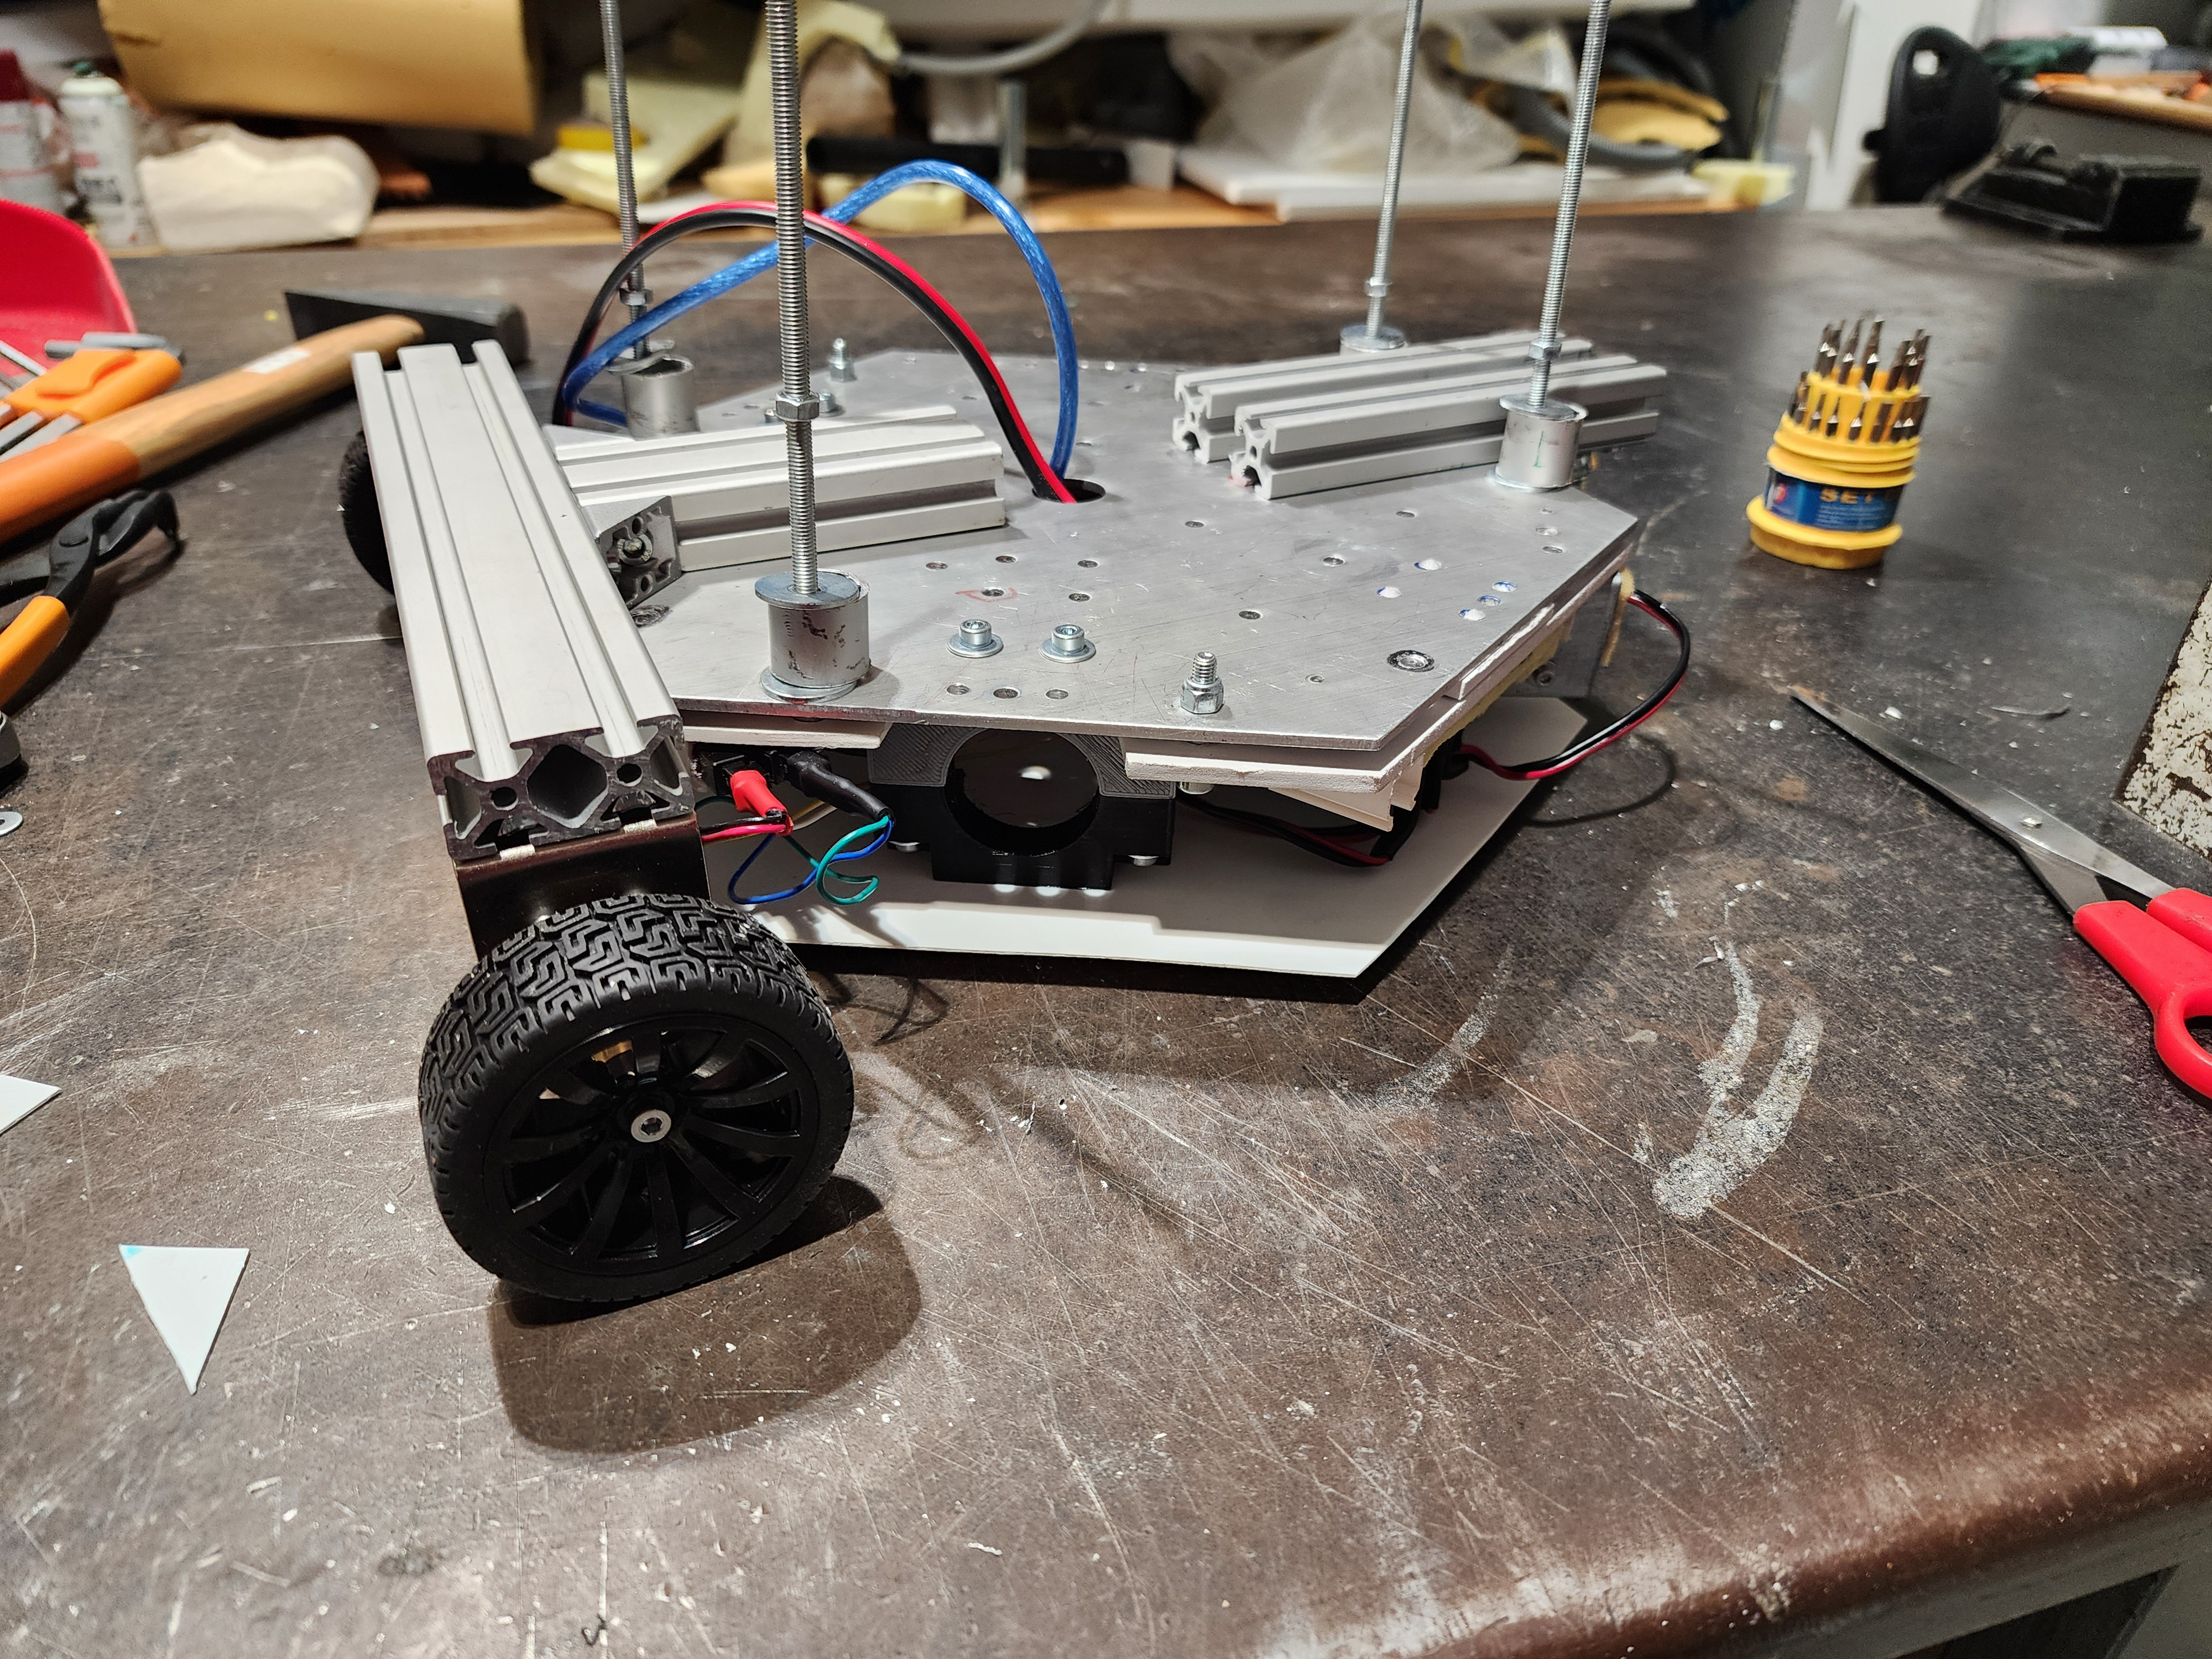
\includegraphics[width=0.7\textwidth]{Images/NewBaseDifferentialDrive.jpg}
    \caption{Complete Differential Drive Base with T-Structure Framework}
    \label{fig:differential_base_complete}
\end{figure}

\subsubsection{Kinematic Simplification and Performance Benefits}

The differential drive design eliminates the mechanical complexity of omnidirectional systems while maintaining the essential mobility requirements for Tino's social interaction scenarios. The two-wheel configuration with rear caster provides stable platform dynamics with reduced component count and simplified maintenance requirements.

Weight distribution optimization utilizes the two front drive wheels to support the majority of Tino's operational weight while the rear caster wheel provides stability without bearing significant driving loads. This configuration eliminates the dragging forces that compromised the original omnidirectional system.

Maneuverability analysis demonstrates that differential drive provides adequate turning capability through differential wheel speed control. The simplified kinematics enable more precise movement control and improved repeatability compared to the three-wheel omnidirectional system.

\subsection{Mechanical Implementation and Structural Modifications}

The mechanical implementation required comprehensive base modification utilizing aluminum Item profiles to create a robust and adjustable platform architecture.

\subsubsection{T-Structure Construction with Aluminum Profiles}

The T-structure design utilizes aluminum Item profiles to create a dynamic and adjustable framework that enables optimal wheel positioning for weight distribution and traction optimization. The modular profile system provides structural rigidity while allowing mechanical adjustments without complete system redesign.
\begin{figure}[H]
    \centering
    \includegraphics[width=0.6\textwidth]{Images/NewBaseDifferentialDrive (5).jpg}
    \caption{Top View of Differential Drive Base with T-Structure}
    \label{fig:differential_base_top}
\end{figure}
Wheel spacing optimization through the adjustable T-structure enables fine-tuning of track width to achieve proper balance and stability characteristics. The aluminum construction provides excellent strength-to-weight ratio while maintaining the structural integrity required for Tino's operational loads.

\begin{figure}[H]
    \centering
    \begin{minipage}{0.45\textwidth}
        \centering
        \includegraphics[width=\textwidth]{Images/NewBaseDifferentialDrive (2).jpg}
        \caption{Differential Drive Base Side View}
        \label{fig:differential_base_side}
    \end{minipage}
    \hfill
    \begin{minipage}{0.45\textwidth}
        \centering
        \includegraphics[width=\textwidth]{Images/NewBaseDifferentialDrive (3).jpg}
        \caption{Caster Wheel supporting Rear of Base}
        \label{fig:differential_base_caster}
    \end{minipage}
\end{figure}

Motor mounting points integrate directly with the Item profile system through custom brackets that provide precise motor alignment and secure attachment. The modular design enables motor replacement or upgrade without structural modifications to the base platform.

\subsubsection{Motor Upgrade and Drive System Enhancement}

The motor upgrade to more powerful units addresses the thermal and torque limitations identified in the original system. The new motors provide enhanced heat dissipation capabilities and higher continuous torque ratings suitable for Tino's operational requirements.

\begin{figure}[H]
    \centering
    \begin{minipage}{0.45\textwidth}
        \centering
        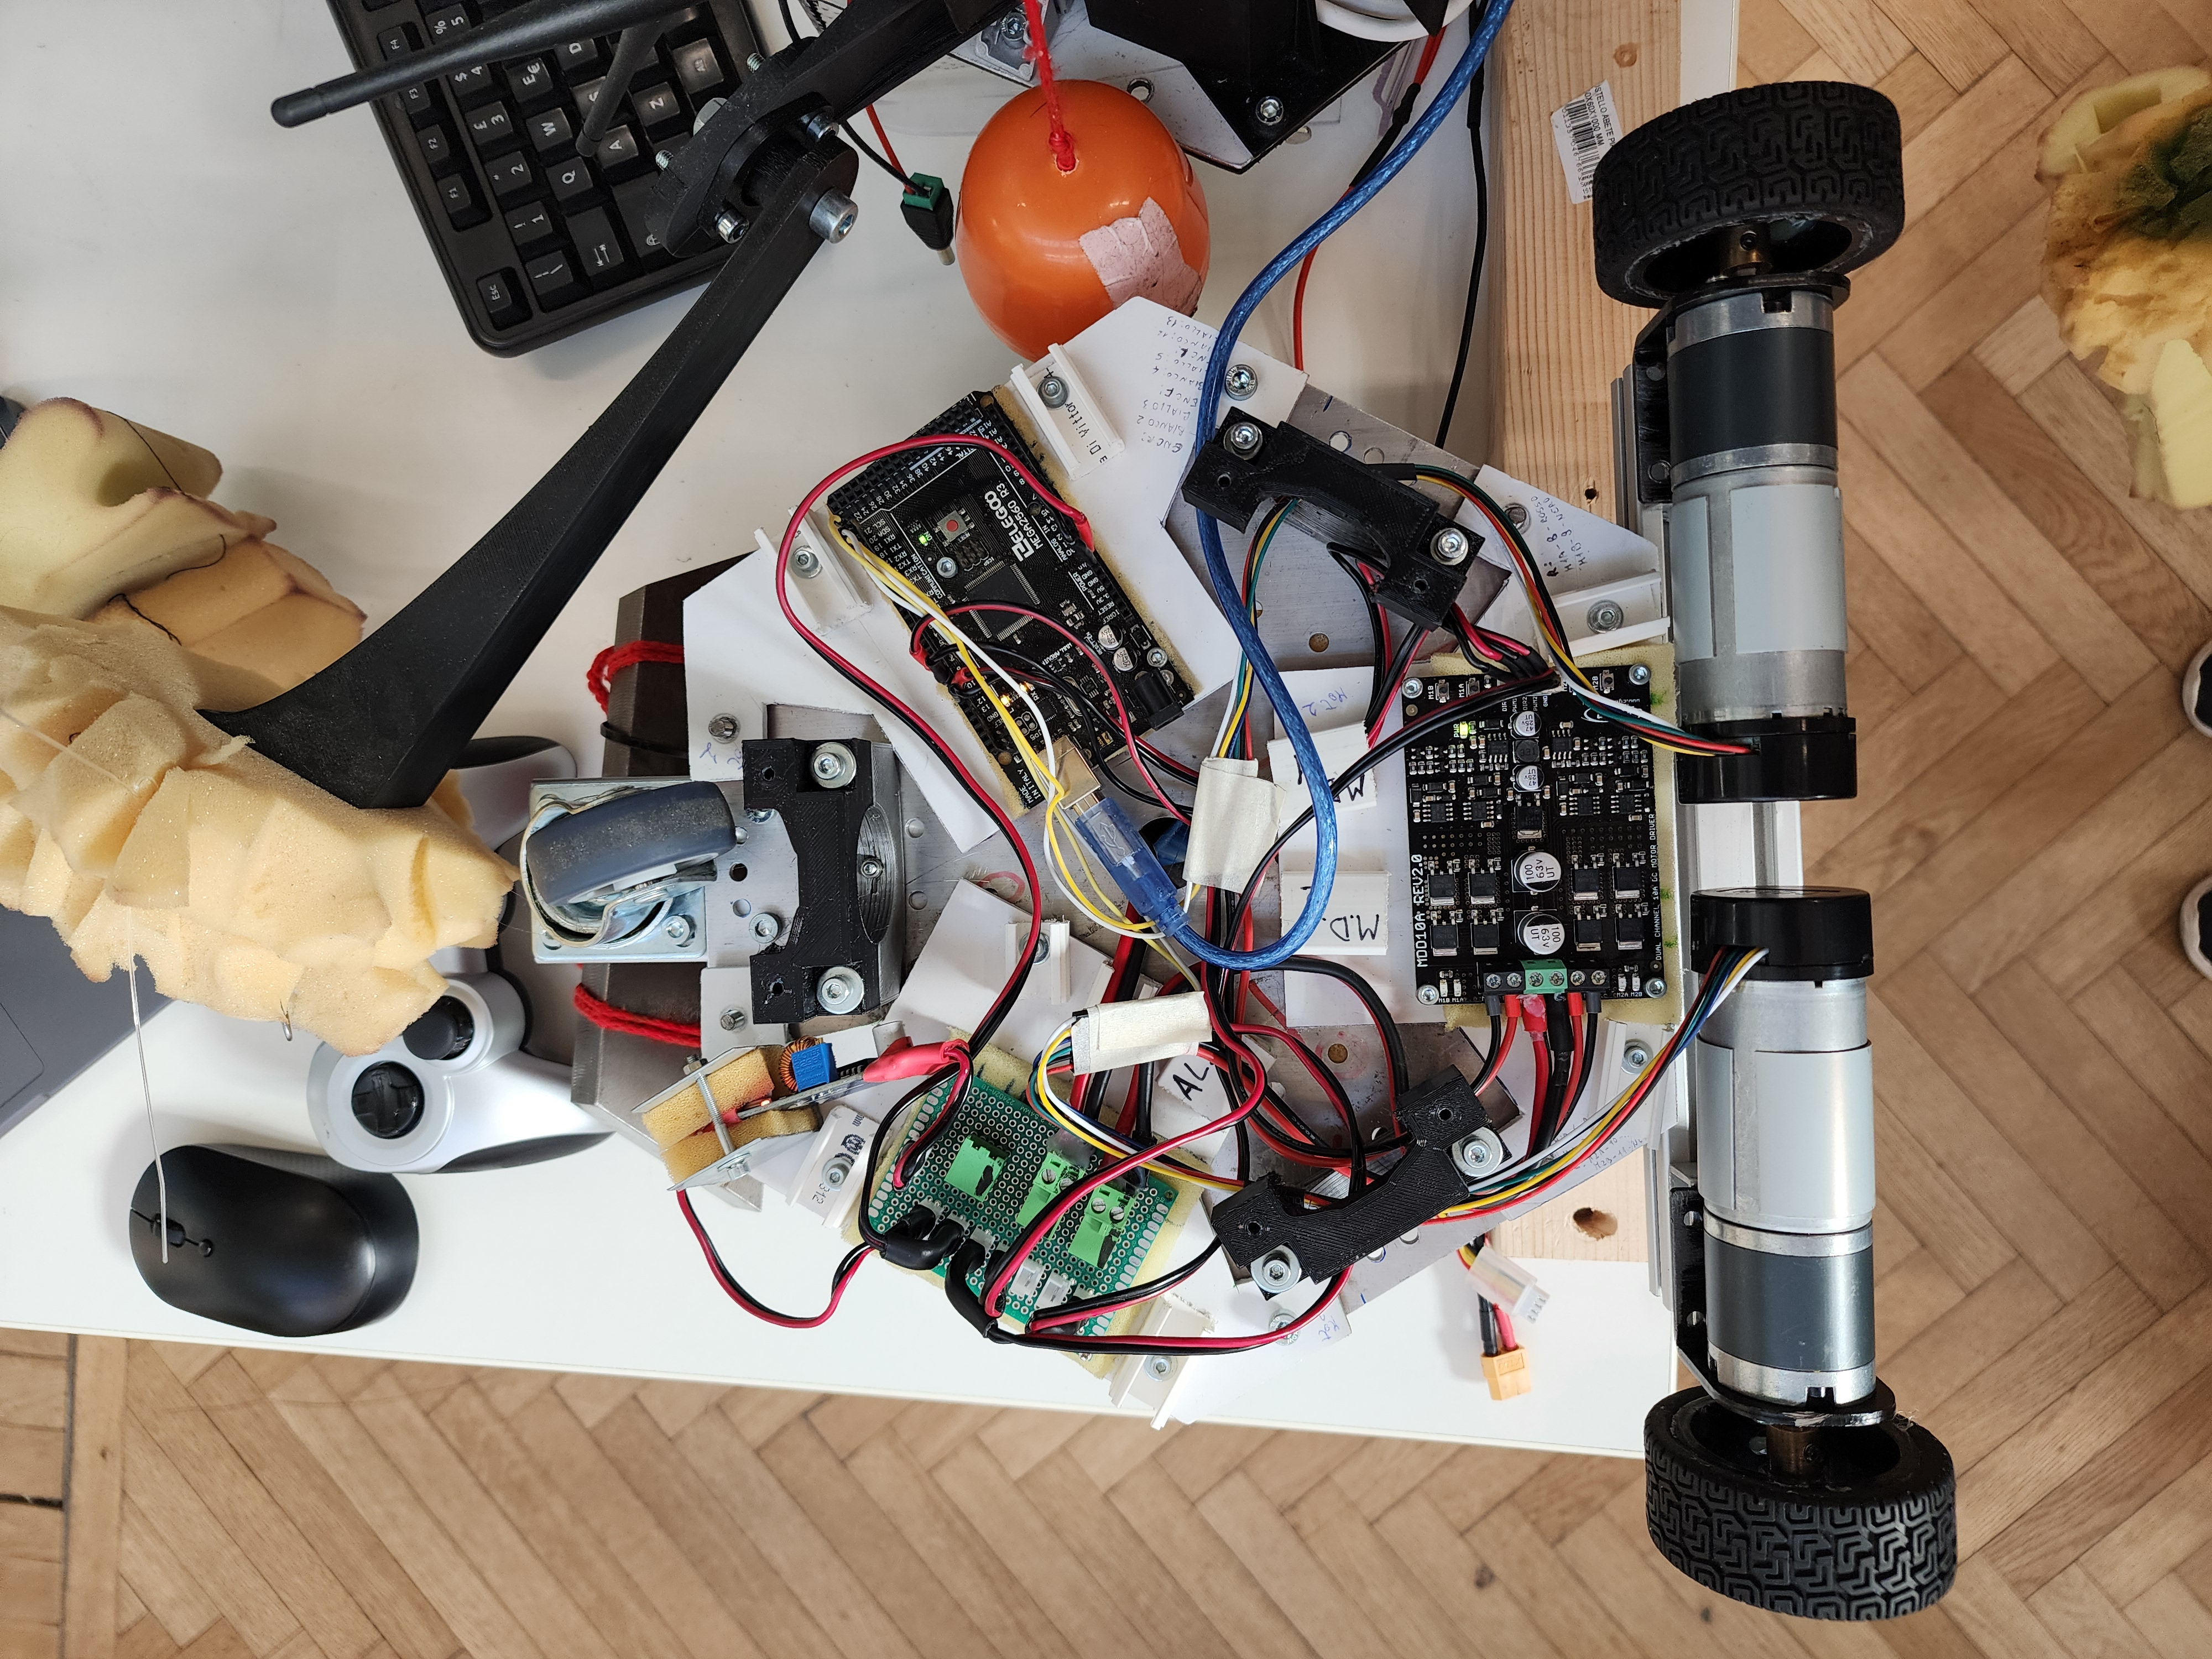
\includegraphics[width=\textwidth,angle=-90]{Images/BaseNewMotors.jpg}
        \caption{Base with New Motors (Top View)}
        \label{fig:base_new_motors}
    \end{minipage}
    \hfill
    \begin{minipage}{0.45\textwidth}
        \centering
        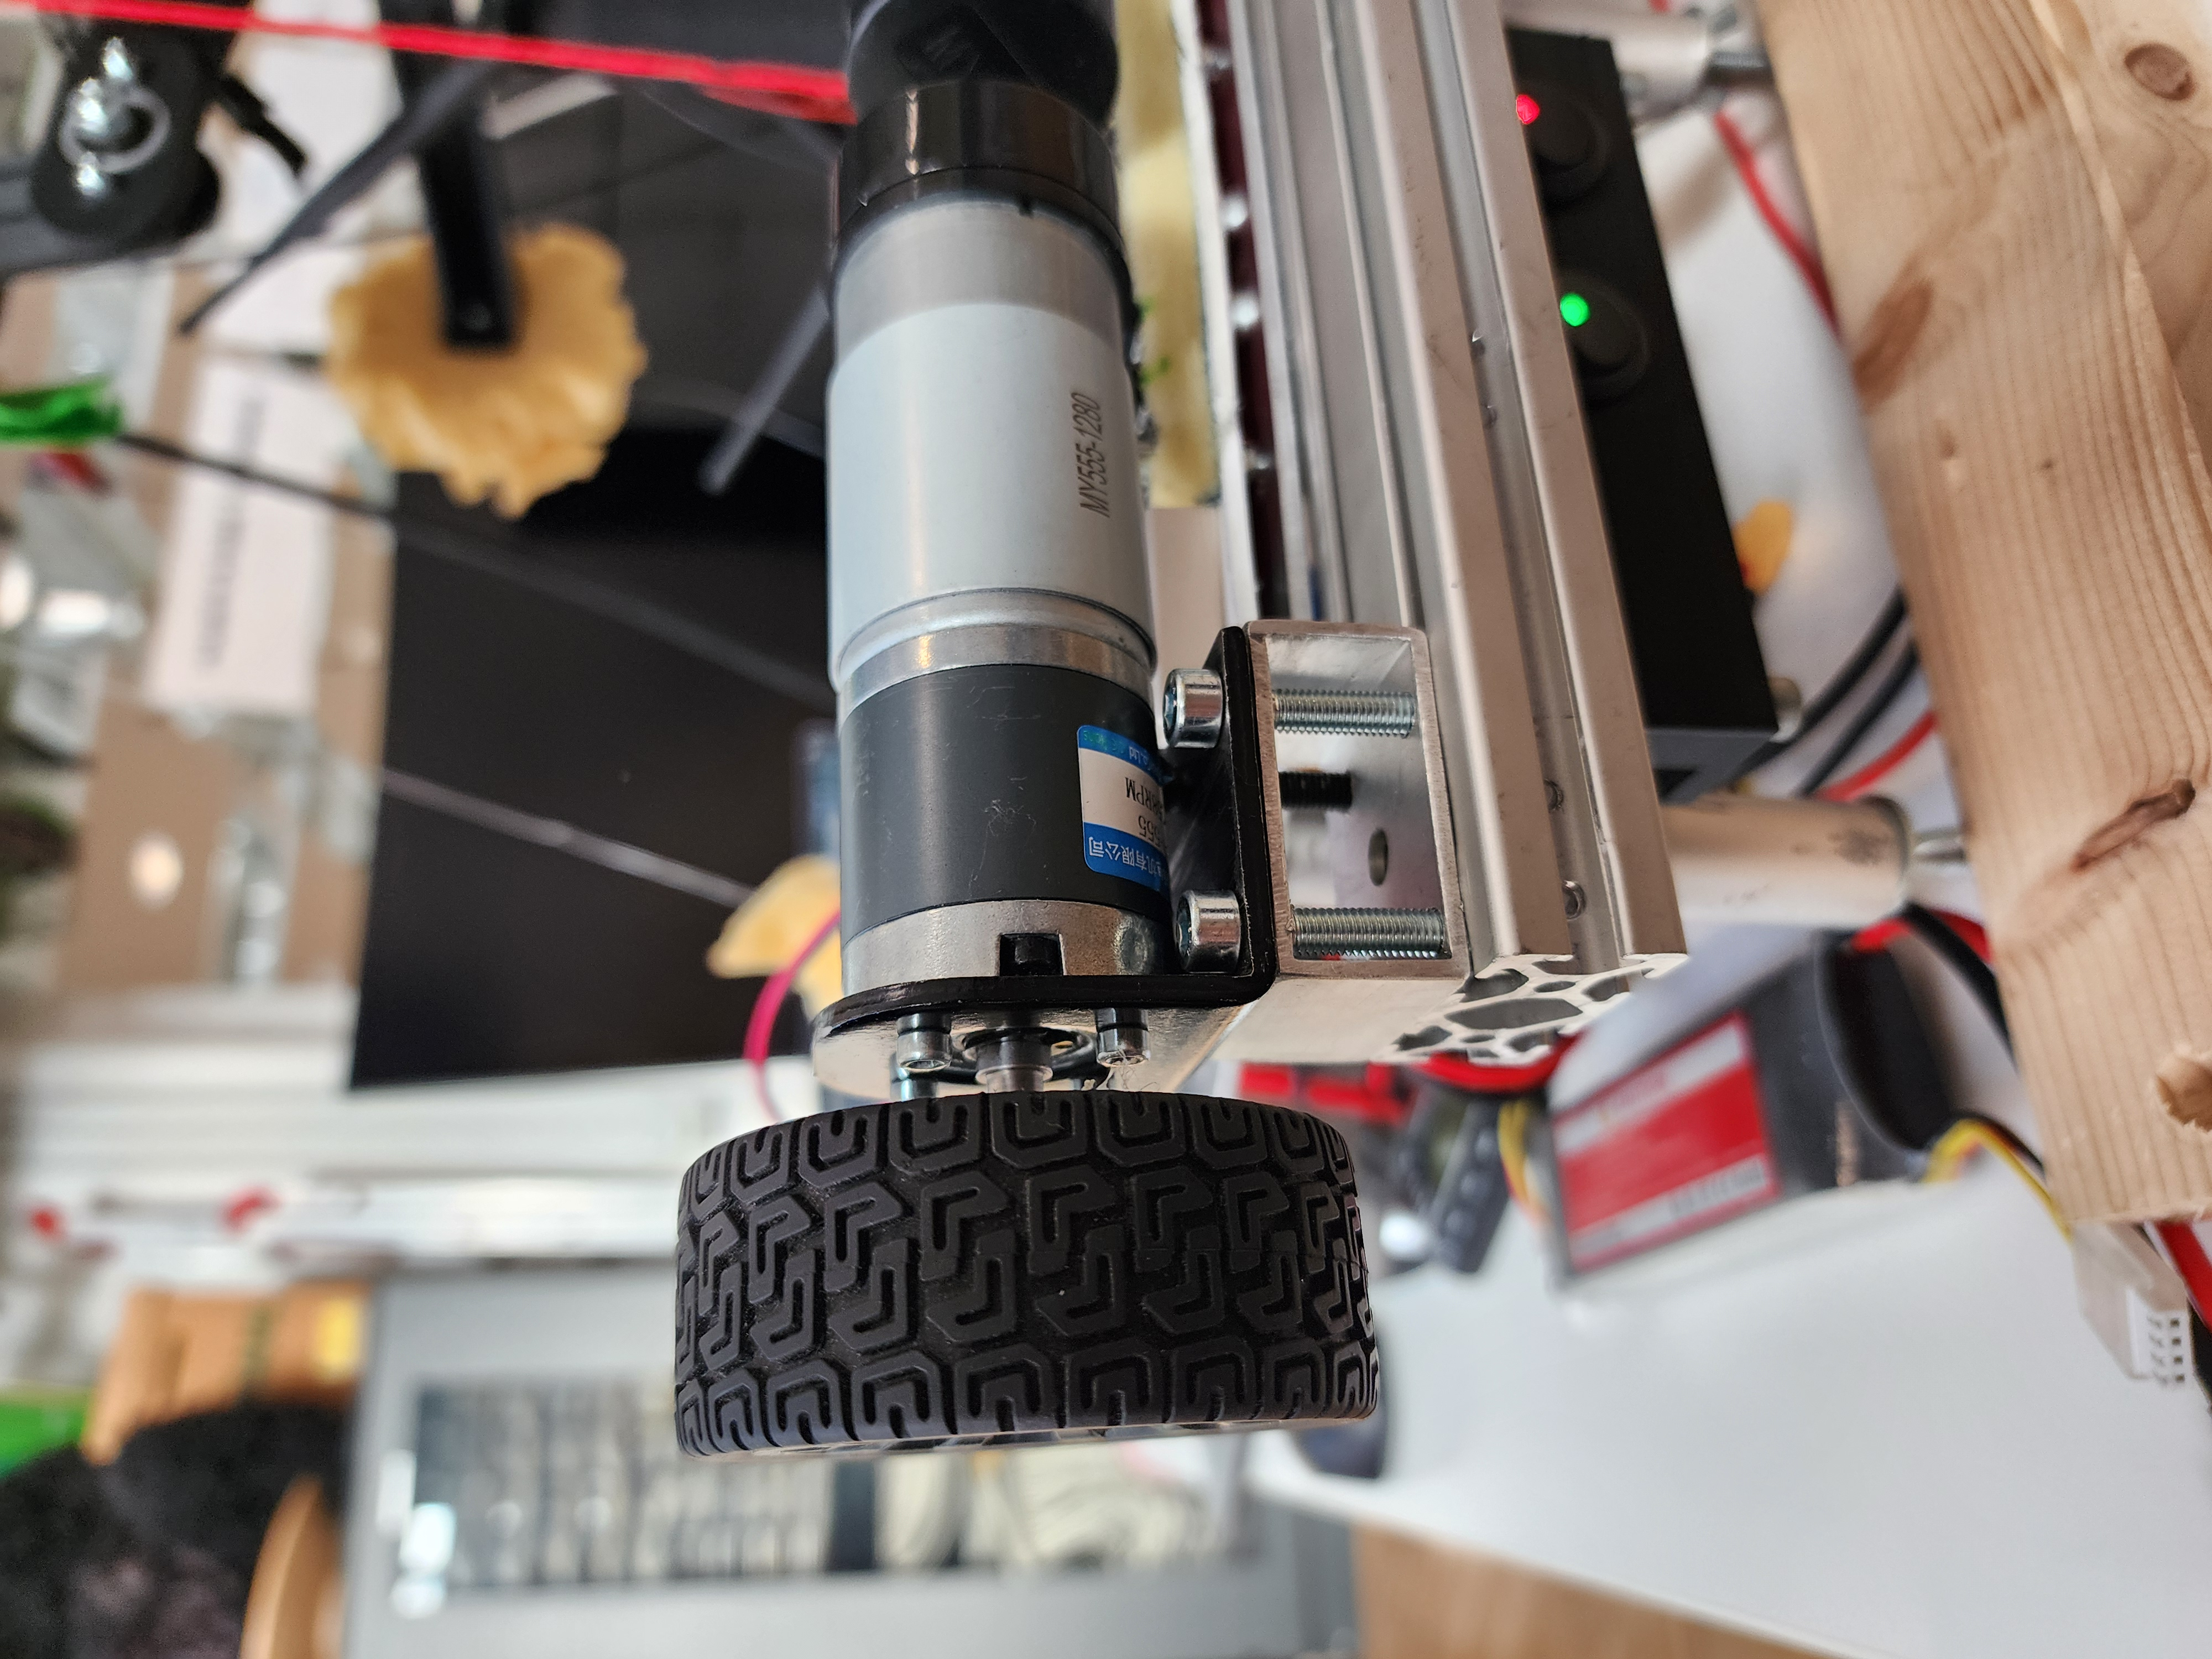
\includegraphics[width=\textwidth,angle=-90]{Images/BaseNewMotors2.jpg}
        \caption{Base with New Motors (Close up Side View)}
        \label{fig:base_new_motors_side}
    \end{minipage}
\end{figure}

Motor driver upgrade to the MDD10A units provides increased current handling capability and enhanced control responsiveness compared to the original dual-driver configuration. The single-driver solution simplifies electrical connections while providing superior performance characteristics for differential drive control.

\subsection{Wheel System Development and Traction Solutions}

The wheel selection and mounting system required iterative development to address the unique challenges of supporting Tino's weight while maintaining reliable traction and durability.

\subsubsection{Wheel Selection Evolution and Testing}

Initial wheel selection utilized plastic wheels with pneumatic rubber tires that provided adequate traction but suffered from hub failure under operational loads. The plastic hub construction proved inadequate for the sustained loading conditions, requiring multiple repairs and replacements during system development.

Tire debeading issues occurred when the rubber tire separated from the plastic hub due to inadequate bonding strength under operational stress. Multiple repair approaches were evaluated, including hot-glue reinforcement that provided temporary solutions but required periodic maintenance.

Wheel hub reinforcement through hot-glue filling addressed the structural weakness in the plastic hub construction. This solution proved effective in preventing debeading while maintaining adequate traction characteristics, though it represents a temporary fix requiring future wheel system upgrade.

\begin{figure}[H]
    \centering
    \begin{subfigure}{0.45\textwidth}
        \centering
        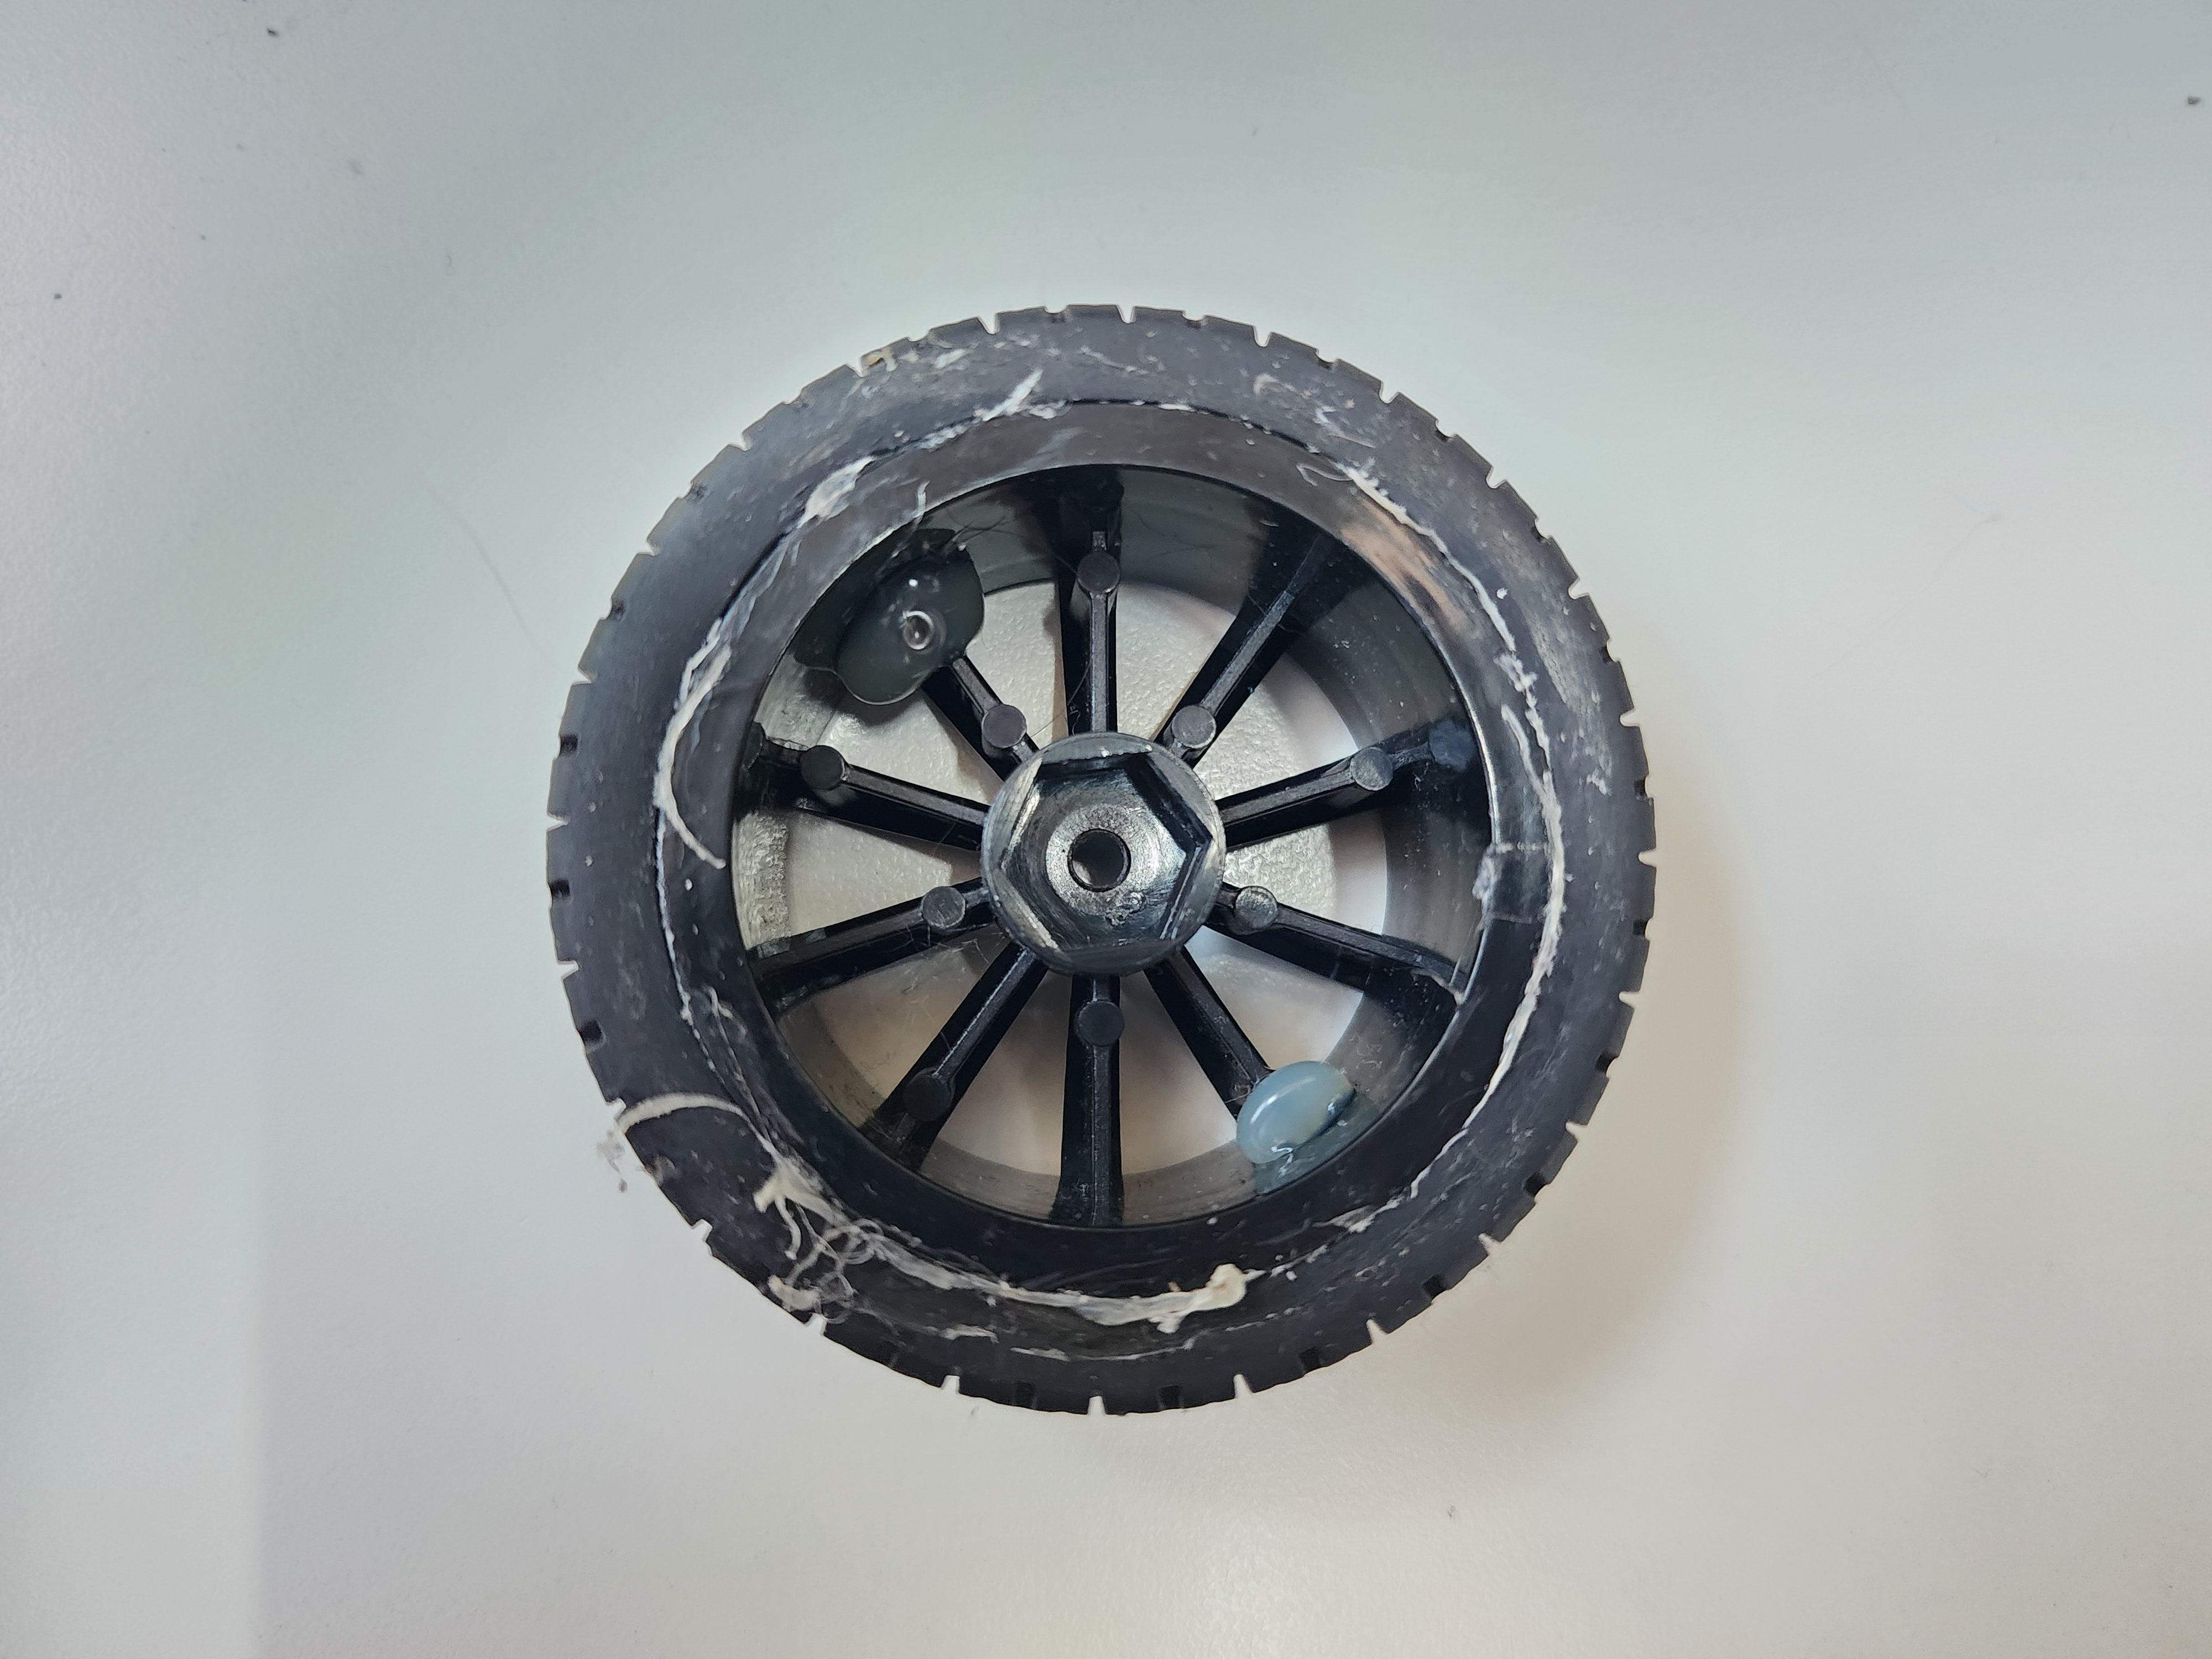
\includegraphics[width=\textwidth]{Images/WheelSilicona (3).jpg}
        \caption{Wheel Front View}
        \label{fig:wheel_hotglue}
    \end{subfigure}
    \hfill
    \begin{subfigure}{0.45\textwidth}
        \centering
        \includegraphics[width=\textwidth]{Images/WheelSilicona.jpg}
        \caption{Wheel Mounted on Motor Shaft}
        \label{fig:wheel_silicone}
    \end{subfigure}
    \caption{Wheel with Hot-Glue Filled Tires}
    \label{fig:combined}
\end{figure}

\subsubsection{Fabric Protection and Bumper Implementation}

Fabric interference prevention required the implementation of protective bumpers to prevent Tino's fabric covering from interfering with wheel operation. The bumper design provides physical separation between the moving wheels and the flexible fabric structure.

\begin{figure}[H]
    \centering
    \includegraphics[height=6cm,angle=-90]{Images/WheelVSFabric (2).jpg}
    \caption{Wheel vs Fabric Interference}
    \label{fig:wheel_vs_fabric}
\end{figure}

Bumper effectiveness testing demonstrated successful prevention of fabric entanglement in most operational scenarios, though some edge cases still require operator attention. The bumper system represents a practical solution that addresses the majority of fabric interference issues without compromising Tino's aesthetic design.

\begin{figure}[H]
    \centering
    \begin{minipage}{0.45\textwidth}
        \centering
        \includegraphics[width=\textwidth]{Images/TinoBumper (4).jpg}
        \caption{Tino Bumper Front View}
        \label{fig:tino_bumper_front}
    \end{minipage}
    \hfill
    \begin{minipage}{0.45\textwidth}
        \centering
        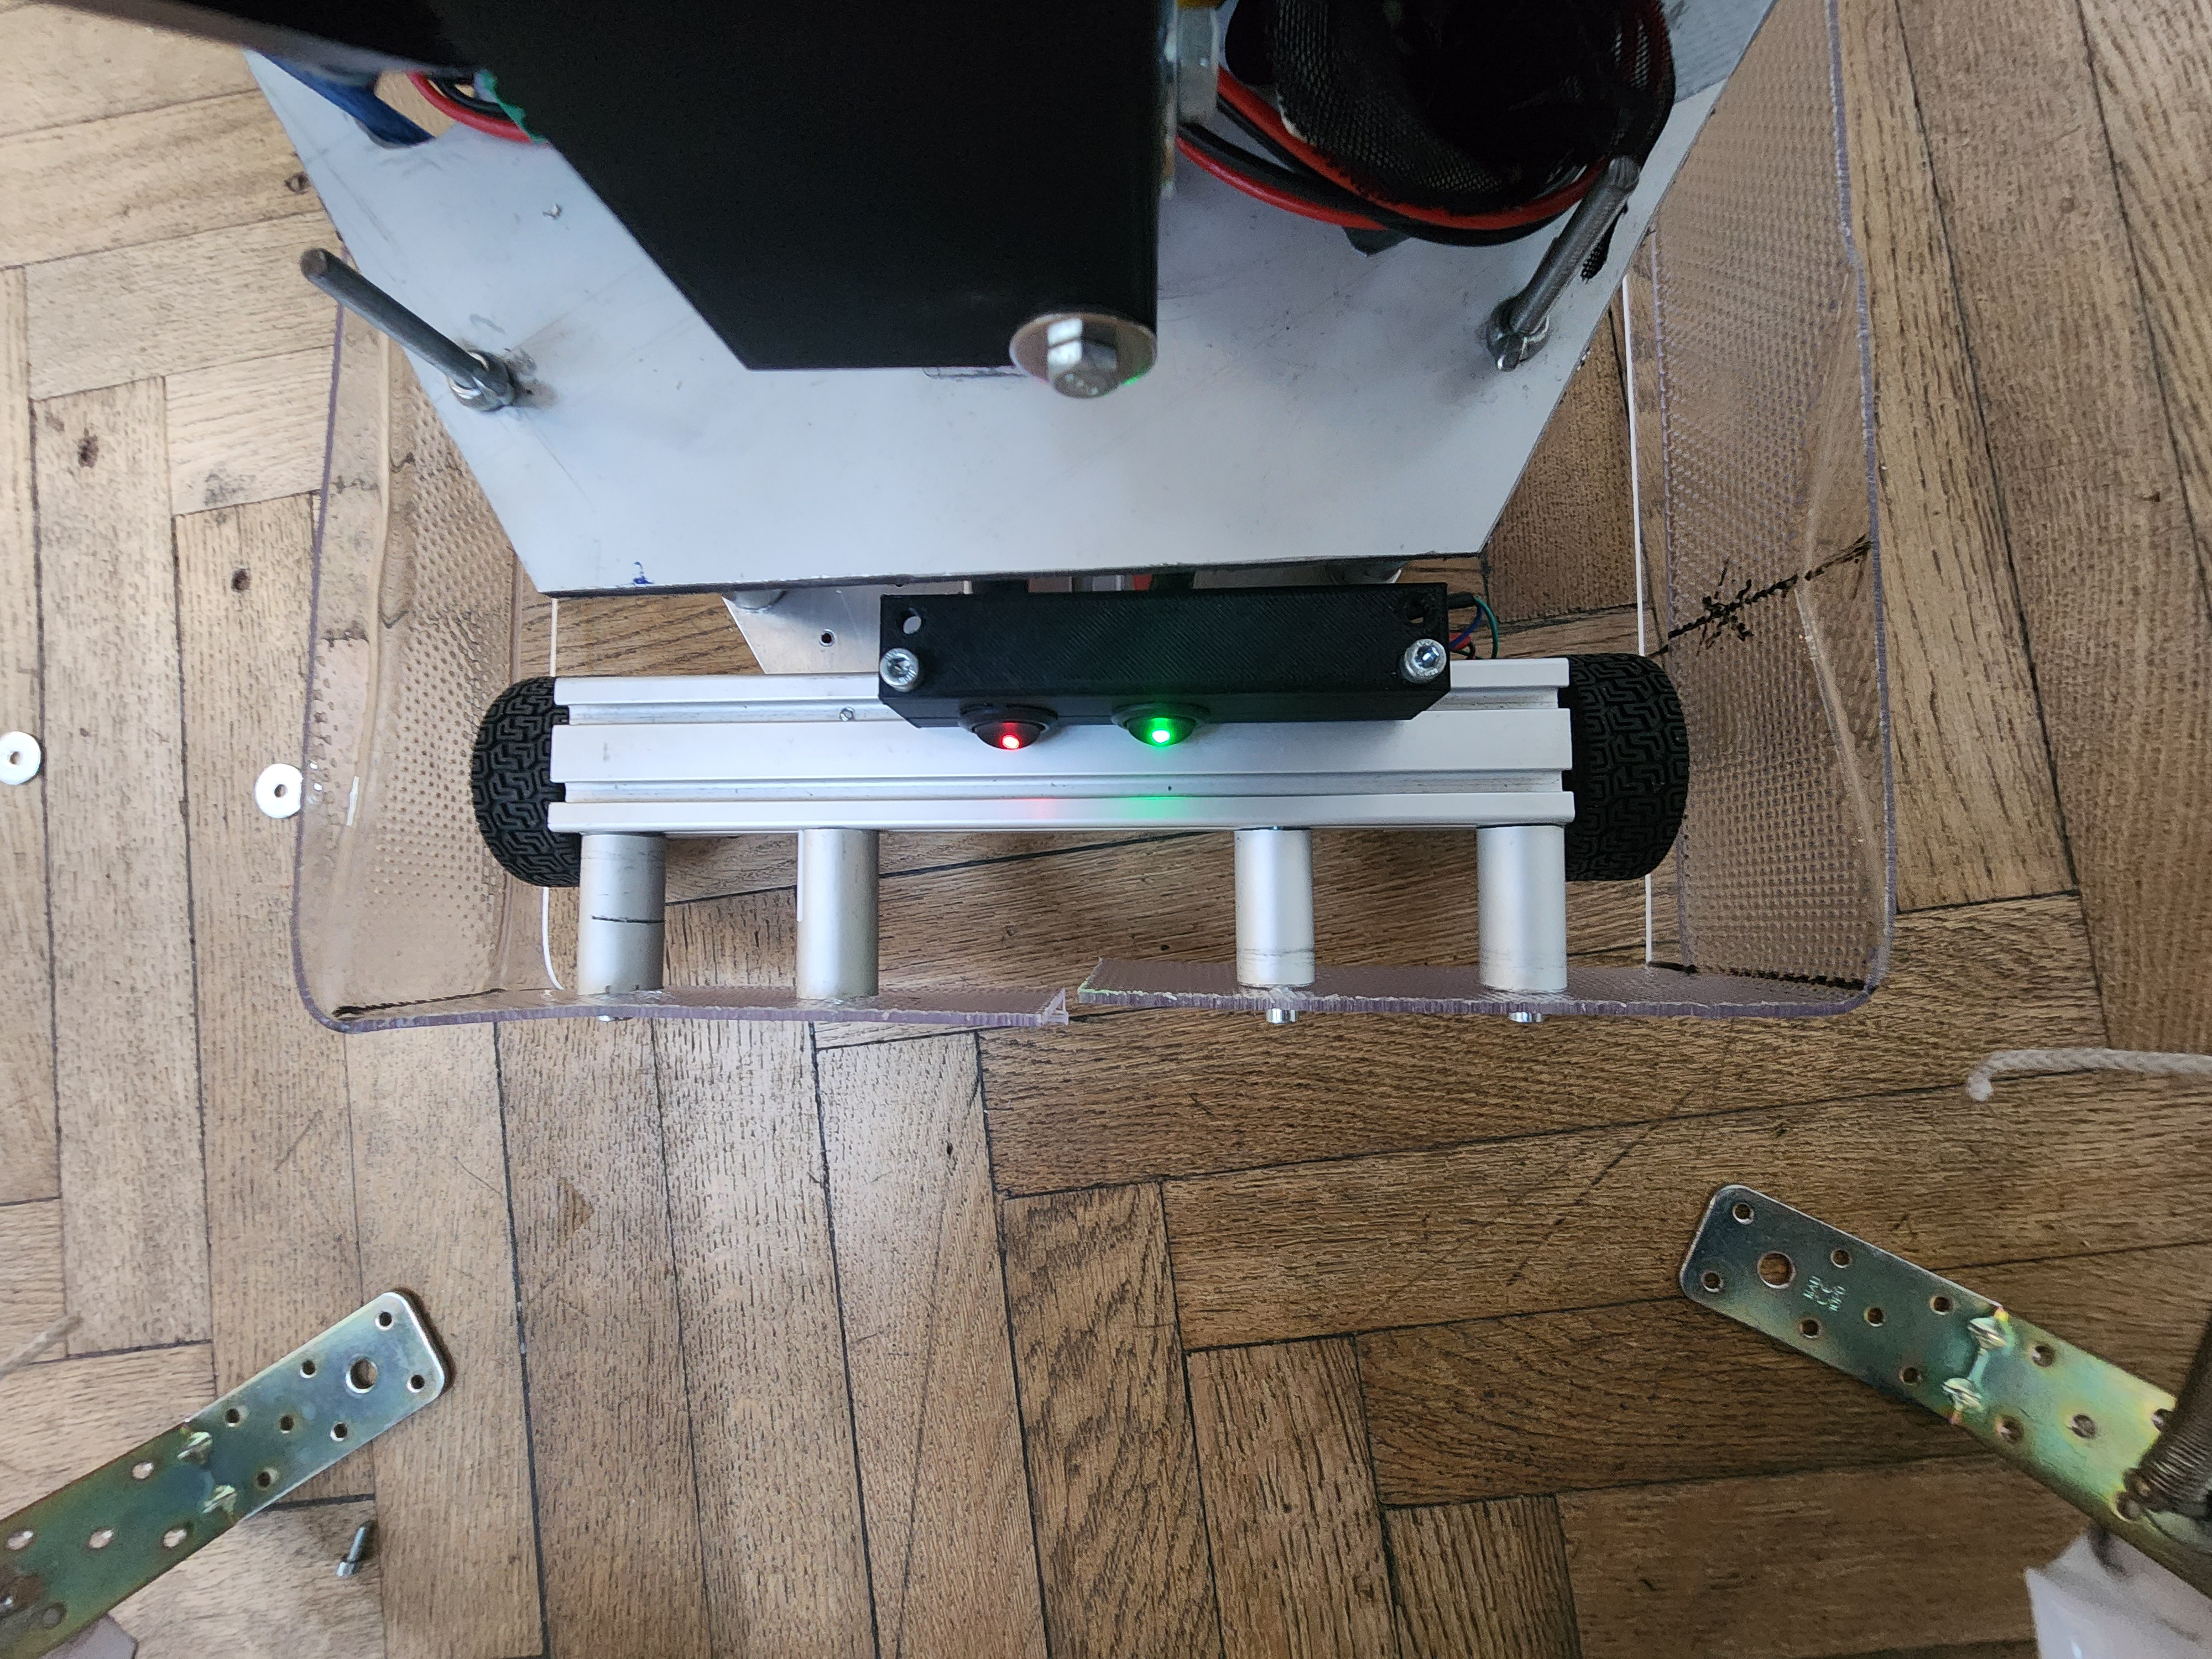
\includegraphics[width=\textwidth]{Images/TinoBumper (5).jpg}
        \caption{Tino Bumper Top View}
        \label{fig:tino_bumper_top}
    \end{minipage}
\end{figure}

\subsection{Control System Adaptation for Differential Drive}

\begin{figure}[H]
    \centering    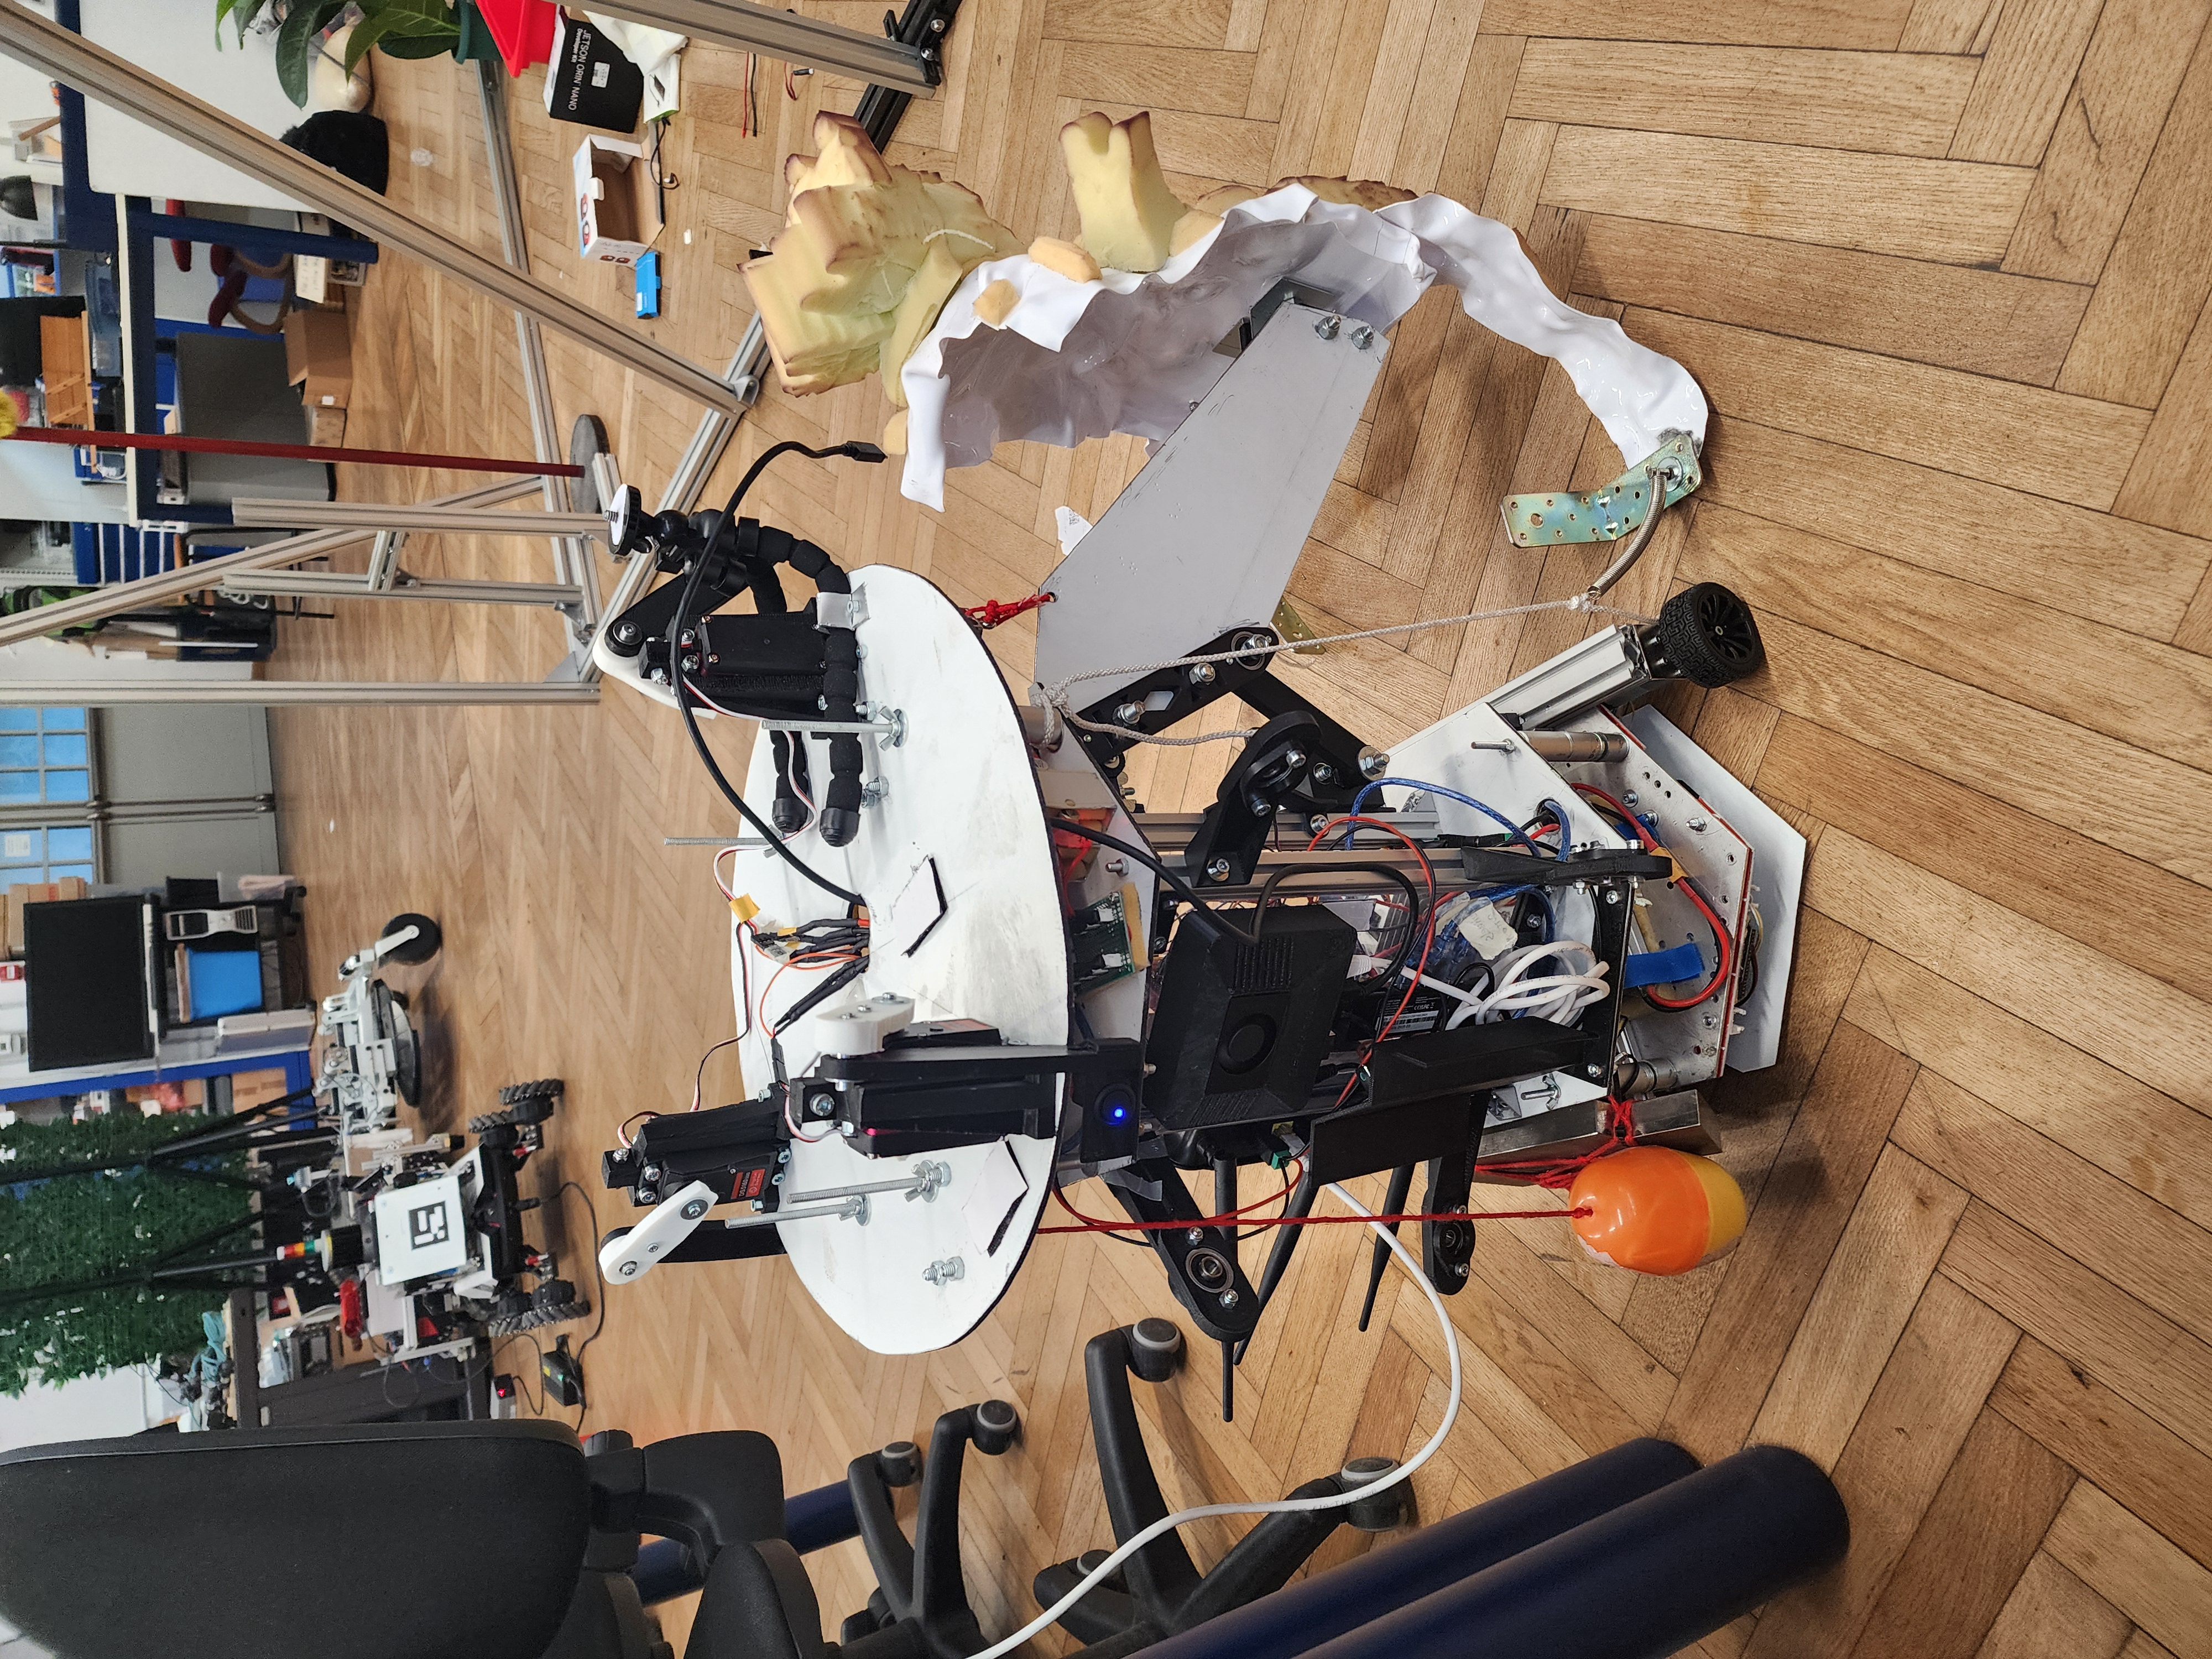
\includegraphics[width=0.8\textwidth]{Images/TinoOnNewBase.jpg}
    \caption{Tino's new Base}
    \label{fig:tino_on_new_base}
\end{figure}

The control system required comprehensive modification to support differential drive kinematics while maintaining compatibility with existing command interfaces and synchronization with the foot movement.

\subsubsection{Custom PID Controller Implementation}

The PID controller development specifically targets differential drive characteristics, replacing the VirHas library with custom control algorithms optimized for Tino's platform. The implementation utilizes classical PID control with Kp=7.3, Ki=5.6, and Kd=0.2 parameters tuned specifically for the MDD10A motor drivers and Tino's mechanical characteristics.

Motor speed calculation employs encoder feedback with 1920 pulses per revolution (PPR) encoders to determine actual wheel speed  in rad/s. The \texttt{getMotorSpeed()} function calculates instantaneous speed based on encoder position changes over time intervals, enabling closed-loop speed control for precise movement execution.

The \texttt{updatePid()} function implements the complete PID algorithm with integral term reset on setpoint changes to prevent windup, derivative calculation for damping, and output limiting to ±255 PWM range. This ensures stable motor control without oscillation while maintaining responsive movement characteristics.

Atomic movement control integrates with the PID system through the \texttt{updateBaseMovementByTime()} function that manages four distinct movement states: resting (0), little push (1), timing preparation (2), and coordinated forward movement (3). Each state implements specific timing profiles and movement patterns that support synchronized leg-base coordination for VR integration.

The movement state machine ensures atomic operation completion where each movement phase must finish before accepting new commands, preventing interrupted motions that could compromise synchronized robot behavior. State transitions include proper timing validation and pending command management for seamless VR user interaction.

\section{Power Supply System Redesign for Orin Nano}

The power system redesign addresses the comprehensive requirements of the NVIDIA Orin Nano platform and associated high-performance components, necessitating complete architecture overhaul from the legacy Raspberry Pi power distribution system.

\subsection{Power Requirements Analysis and System Specifications}



\subsubsection{Orin Nano Power Consumption Characteristics}

The Orin Nano requires 19V DC input with power consumption characteristics that reach up to 2A during maximum computational load scenarios including simultaneous SLAM processing, human detection, audio processing, and ROS2 node operation. Typical operational consumption ranges between 1.3A to 1.4A during standard social interaction scenarios.

Power consumption analysis under various operational modes demonstrates peak consumption of 38W during maximum load conditions, with sustained operation typically requiring 25-27W. The power profile exhibits significant variation based on computational load, requiring robust power delivery capable of handling transient peaks without voltage drop.

Computational load correlation shows direct relationship between power consumption and processing intensity, with SLAM operations, TensorRT inference, and audio processing requiring the highest power demands. The variable load characteristics necessitate stable power delivery across the full operational range.

\subsubsection{Auxiliary System Power Requirements}

The Oak-D Pro camera system requires 5V DC input with power consumption up to 5W during high-resolution stereo processing. The camera power can be supplied directly from the Orin Nano USB ports or through dedicated power distribution for enhanced flexibility and reduced main processor loading.

The onboard router system requires 5V DC input for network connectivity and VR communication capabilities. Router power consumption remains relatively constant at approximately 3W during operational periods, providing stable power requirements for system design.

Total system power budget analysis indicates maximum power consumption of approximately 46W under peak operational conditions, with typical sustained operation requiring 33-35W. The power analysis includes safety margins for component aging and environmental variations.

\subsection{DC-DC Converter Implementation and Power Distribution}

The power conversion system utilizes high-efficiency DC-DC converters to transform battery voltage to the multiple voltage levels required by system components.

\subsubsection{Oumefar 12V to 19V Step-Up Converter Selection}

The Oumefar DC-DC step-up converter provides stable 19V output from 12V battery input with efficiency ratings exceeding 85\% across the operational load range. Converter selection prioritized stability, efficiency, and thermal performance under the sustained loading conditions required for social robot operation.

Power delivery stability testing demonstrated consistent voltage regulation within ±2\% across full load range with excellent transient response during computational load variations. Thermal performance analysis shows acceptable operating temperatures during sustained maximum load conditions without additional cooling requirements.

Load regulation characteristics maintain stable 19V output from no-load to maximum current draw, ensuring consistent Orin Nano performance across all operational scenarios. The converter includes overcurrent protection and thermal shutdown features that protect against component failure during fault conditions.

\subsubsection{Secondary Power Rail Implementation}

The 12V to 5V conversion system provides power for auxiliary components including the Oak-D Pro camera and onboard router. The secondary converter selection prioritized efficiency and multiple output capability to support various system components.

Power distribution architecture enables independent power control for auxiliary components, providing flexibility for future system expansion and reduced loading on the primary Orin Nano power rail. The distributed approach improves system reliability by isolating power domains.

Circuit protection includes individual fusing for each power rail and overcurrent protection that prevents system damage during component failure scenarios. The protection scheme enables continued operation of unaffected systems during partial power system failures.

\subsection{Battery System Optimization and Consolidation}

The battery system redesign consolidates multiple power sources while providing enhanced capacity and reliability for extended operational periods.

\subsubsection{Battery Specification and Performance Analysis}

The primary battery system utilizes 5200mAh 80C 11.1V 57.72Wh LiPo batteries that provide the power density and discharge capabilities required for robotic applications. Battery specification analysis demonstrates adequate capacity for 2-3 hours of typical operation with conservative discharge management.

Maximum load operational time calculations indicate approximately 1.37 hours of operation under peak power conditions, though realistic operational scenarios typically achieve 2+ hours due to variable computational loading.

Discharge characteristics analysis demonstrates stable voltage delivery throughout the operational range with minimal voltage drop during high current transients. The high discharge rate capability (80C) ensures stable power delivery during computational peaks without voltage sag.

\subsubsection{Power System Consolidation Strategy}

The system consolidation reduces complexity from four separate battery systems to three integrated power sources, eliminating the dedicated router power bank and USB power bank previously required for Raspberry Pi operation. Consolidation simplifies system startup procedures and reduces component count.

Battery management strategy includes individual monitoring and charging protocols for each power source while maintaining operational independence. The consolidated approach reduces overall system weight while providing enhanced operational capability through optimized power distribution.

Operational startup sequence simplifies through power system consolidation, reducing from multiple power-on procedures to streamlined system activation. The simplified approach reduces operator complexity and potential startup errors during experimental scenarios.

\subsection{Cable Harness Redesign and Integration}

The cable harness redesign eliminates legacy connections while implementing proper power distribution for the enhanced system architecture.

\subsubsection{Legacy Connection Removal and Modernization}

The cable harness modification removes obsolete USB-A and USB-C connections that were utilized for Raspberry Pi power delivery, replacing them with proper 12V distribution and 19V DC jack connectivity optimized for Orin Nano requirements. Connector selection prioritizes reliability and ease of maintenance.

Cable routing optimization reduces electromagnetic interference and mechanical stress while providing secure connections throughout the system. Harness design includes service loops and strain relief that accommodate system maintenance without cable damage.

Connector standardization utilizes consistent connector types throughout the system to simplify maintenance and reduce spare parts requirements. Standardization also reduces connection errors during system assembly and troubleshooting procedures.

\subsubsection{Power Distribution Architecture}

The 12V input distribution system provides primary power for both the step-up converter and the secondary 5V converter, enabling efficient power utilization from the primary battery source. Distribution includes proper circuit protection and monitoring capabilities.

The 19V DC jack implementation provides secure power connection to the Orin Nano with proper mechanical support and electrical contact reliability. Jack selection includes locking mechanisms that prevent accidental disconnection during operation.

Future expansion capabilities include additional power distribution points for system upgrades and experimental equipment integration. The modular power architecture supports system enhancement without complete harness redesign.

\section{Stewart Platform Head Mechanism Improvements}

The Stewart platform head mechanism underwent iterative design improvements to address systematic reliability issues and enhance performance under the operational loads encountered during social robot interaction scenarios.

\subsection{Original System Analysis and Failure Modes}

The original Stewart platform implementation exhibited multiple failure modes that compromised head movement precision and system reliability during extended operational periods.

\subsubsection{Servo Axis Misalignment Problems}

The original design suffered from servo axis misalignment that created excessive stress concentrations on servo motor internals during head movement operations. Force analysis revealed that head loads were transmitted directly through servo shafts rather than through the structural framework, creating potential failure-prone stress concentrations.

The misalignment created moment arms that amplified forces applied to servo components, requiring design revision to prevent potential servo damage. The servo axis alignment improvement was implemented as a preventive measure to ensure reliable long-term operation.

Mechanical analysis demonstrated that proper force transmission should flow through the head structure rather than servo mechanisms, necessitating fundamental design revision to achieve reliable operation under Tino's operational requirements.

\subsubsection{Structural Flexibility and Arm Failures}

The connecting arms exhibited excessive structural flexibility that reduced head positioning precision and contributed to mechanical instability during movement sequences. Flexibility analysis revealed inadequate stiffness-to-weight ratio in the original arm design, creating undesired compliance in the kinematic chain.

Repeated arm failures occurred due to inadequate load distribution and material selection that could not withstand the combination of static head weight and dynamic movement forces. Failure analysis identified stress concentration points where 3D printed components experienced crack initiation and propagation.

Material selection limitations in PLA printing created brittleness under repeated loading cycles, with failure modes including layer delamination and stress cracking at critical load transfer points. The original material selection proved inadequate for the sustained loading requirements of social robot head movement.

\subsection{First Design Iteration: Servo Axis Alignment}

The first improvement iteration focused on servo axis alignment to redirect forces through proper load paths while maintaining the existing bearing-based connection system.

\begin{figure}[H]
    \centering
    \includegraphics[height=6cm, angle=-90]{Images/HeadArmV2.jpg}
    \caption{Head Arm V1 Design}
    \label{fig:head_arm_v1}
\end{figure}

\subsubsection{Force Path Optimization}

The servo axis alignment improvement redirected head loads through the structural framework rather than servo mechanisms, reducing stress concentrations in servo internal components. Force analysis demonstrated significant reduction in lateral servo loading through proper geometric alignment.

Structural load distribution optimization utilized improved geometry to distribute head weight and movement forces across the Stewart platform structure. Load path analysis verified proper force transmission through structural components rather than servo mechanisms.

Performance evaluation demonstrated reduced servo stress indicators and improved movement precision, though structural flexibility issues remained due to the retained bearing connection system on the servo side of each arm.

\subsubsection{ 3D Printed Component Enhancement}

Enhanced PLA arm geometry provided improved load distribution through optimized cross-sectional design and stress concentration reduction. Geometric optimization utilized finite element analysis principles to identify optimal material distribution within manufacturing constraints.

Print orientation optimization aligned layer structure with primary stress directions to maximize strength characteristics within PLA material limitations. Layer orientation analysis demonstrated significant strength improvement through proper print setup procedures.

Initial performance testing showed improved reliability and reduced failure frequency, though continued structural flexibility limited overall system performance improvement. The partial solution validated the design approach while highlighting remaining system limitations.

\subsection{Persistent Flexibility Issues and Continued Arm Failures}

Despite the servo axis alignment improvements implemented in the first design iteration, the Stewart platform continued to experience significant structural flexibility problems that ultimately led to repeated arm failures during extended operational periods.

\begin{figure}[H]
    \centering
    \includegraphics[height=6cm, angle=-90]{Images/HeadArmFailure (2).jpg}
    \caption{Head Arm Failure after Extended Use}
    \label{fig:head_arm_failure}
\end{figure}

\subsubsection{Bearing Connection System Limitations}

The retained bearing connection system on the servo side of each arm introduced excessive compliance that compromised head positioning precision and contributed to continued mechanical instability. The bearing housings, while providing smooth articulation, created weak points in the structural chain that allowed unwanted deflection under operational loads.

Failure analysis revealed that the 3D printed bearing housings could not adequately transfer forces between the improved servo connections and the head platform. The plastic bearing housing geometry, despite geometric optimization, remained insufficient to handle the combination of static head weight and dynamic movement forces encountered during typical social robot operation.

Repeated stress cycling during normal head movement operations caused progressive degradation of the bearing connection points, leading to increased play and eventual structural failure. The bearing system's inherent flexibility, while beneficial for smooth movement, created unacceptable structural compliance that compromised system reliability.

\begin{figure}[htbp]
    \centering
    \begin{minipage}{0.45\textwidth}
        \centering
        \includegraphics[width=\textwidth]{Images/HeadArmFailure (3).jpg}
        \caption{Servo Side Bearing Connection Failure}
        \label{fig:servo_bearing_failure}
    \end{minipage}
    \hfill
    \begin{minipage}{0.45\textwidth}
        \centering
        \includegraphics[width=\textwidth]{Images/HeadArmFailure.jpg}
        \caption{Head Arm Failure after Extended Use}
        \label{fig:head_arm_failure}
    \end{minipage}
\end{figure}

\subsubsection{Material and Design Constraint Analysis}

The fundamental limitation resided in the conflict between the need for smooth articulation and structural rigidity within the constraints of 3D printed PLA construction. PLA material properties, while adequate for static structural components, proved insufficient for dynamic load-bearing connections subjected to repeated stress cycles.

Print resolution limitations prevented the creation of bearing surfaces with sufficient precision and durability for sustained operation under Tino's operational loads. Layer adhesion characteristics in PLA created inherent weak points at stress concentration areas around bearing connection points.

The design iteration validated the servo alignment approach while conclusively demonstrating that bearing-based connections could not provide the structural integrity required for reliable long-term operation. These findings necessitated a fundamental redesign approach that would eliminate the problematic bearing connections entirely.

\subsection{Final Design Implementation: Rod End Integration}

The final design iteration addressed remaining flexibility issues through the adoption of rod end (heim joint) connections on both ends of each Stewart platform arm.

\begin{figure}[H]
    \centering
    \includegraphics[height=6cm]{Images/NewHeadDoubleJoint (4).jpg}
    \caption{Head Arm V2 Design with Rod Ends}
    \label{fig:head_arm_v2}
\end{figure}

\subsubsection{Rod End Selection and Implementation}

Research into Stewart platform best practices identified rod end connections as the standard solution for eliminating binding while allowing proper articulation throughout the movement range. Rod end selection prioritized load capacity, articulation range, and integration with existing servo and head mounting points.

The rod end implementation utilizes metal heim joints that provide superior strength and durability compared to the original bearing system that used metal bearings encased within 3D printed components. Metal construction eliminates the brittleness and wear issues encountered with the printed bearing housings.

Joint articulation characteristics enable free rotation in all necessary axes while providing positive mechanical connection between arm segments. The rod end design eliminates binding forces that contributed to servo stress and movement precision issues.

\subsubsection{Mechanical Trade-offs and Performance Characteristics}

The rod end implementation introduces acceptable head wobble during stationary periods due to the free articulation provided by the heim joints. Analysis indicates this wobble may actually enhance Tino's expressive capabilities by providing natural movement characteristics.

\begin{figure}[H]
    \centering
    \begin{minipage}{0.45\textwidth}
        \centering
        \includegraphics[width=\textwidth]{Images/NewHeadDoubleJoint (6).jpg}
        \caption{Head Arm with Rod Ends (Sway to right)}
        \label{fig:head_arm_rod_end_right}
    \end{minipage}
    \hfill
    \begin{minipage}{0.45\textwidth}
        \centering
        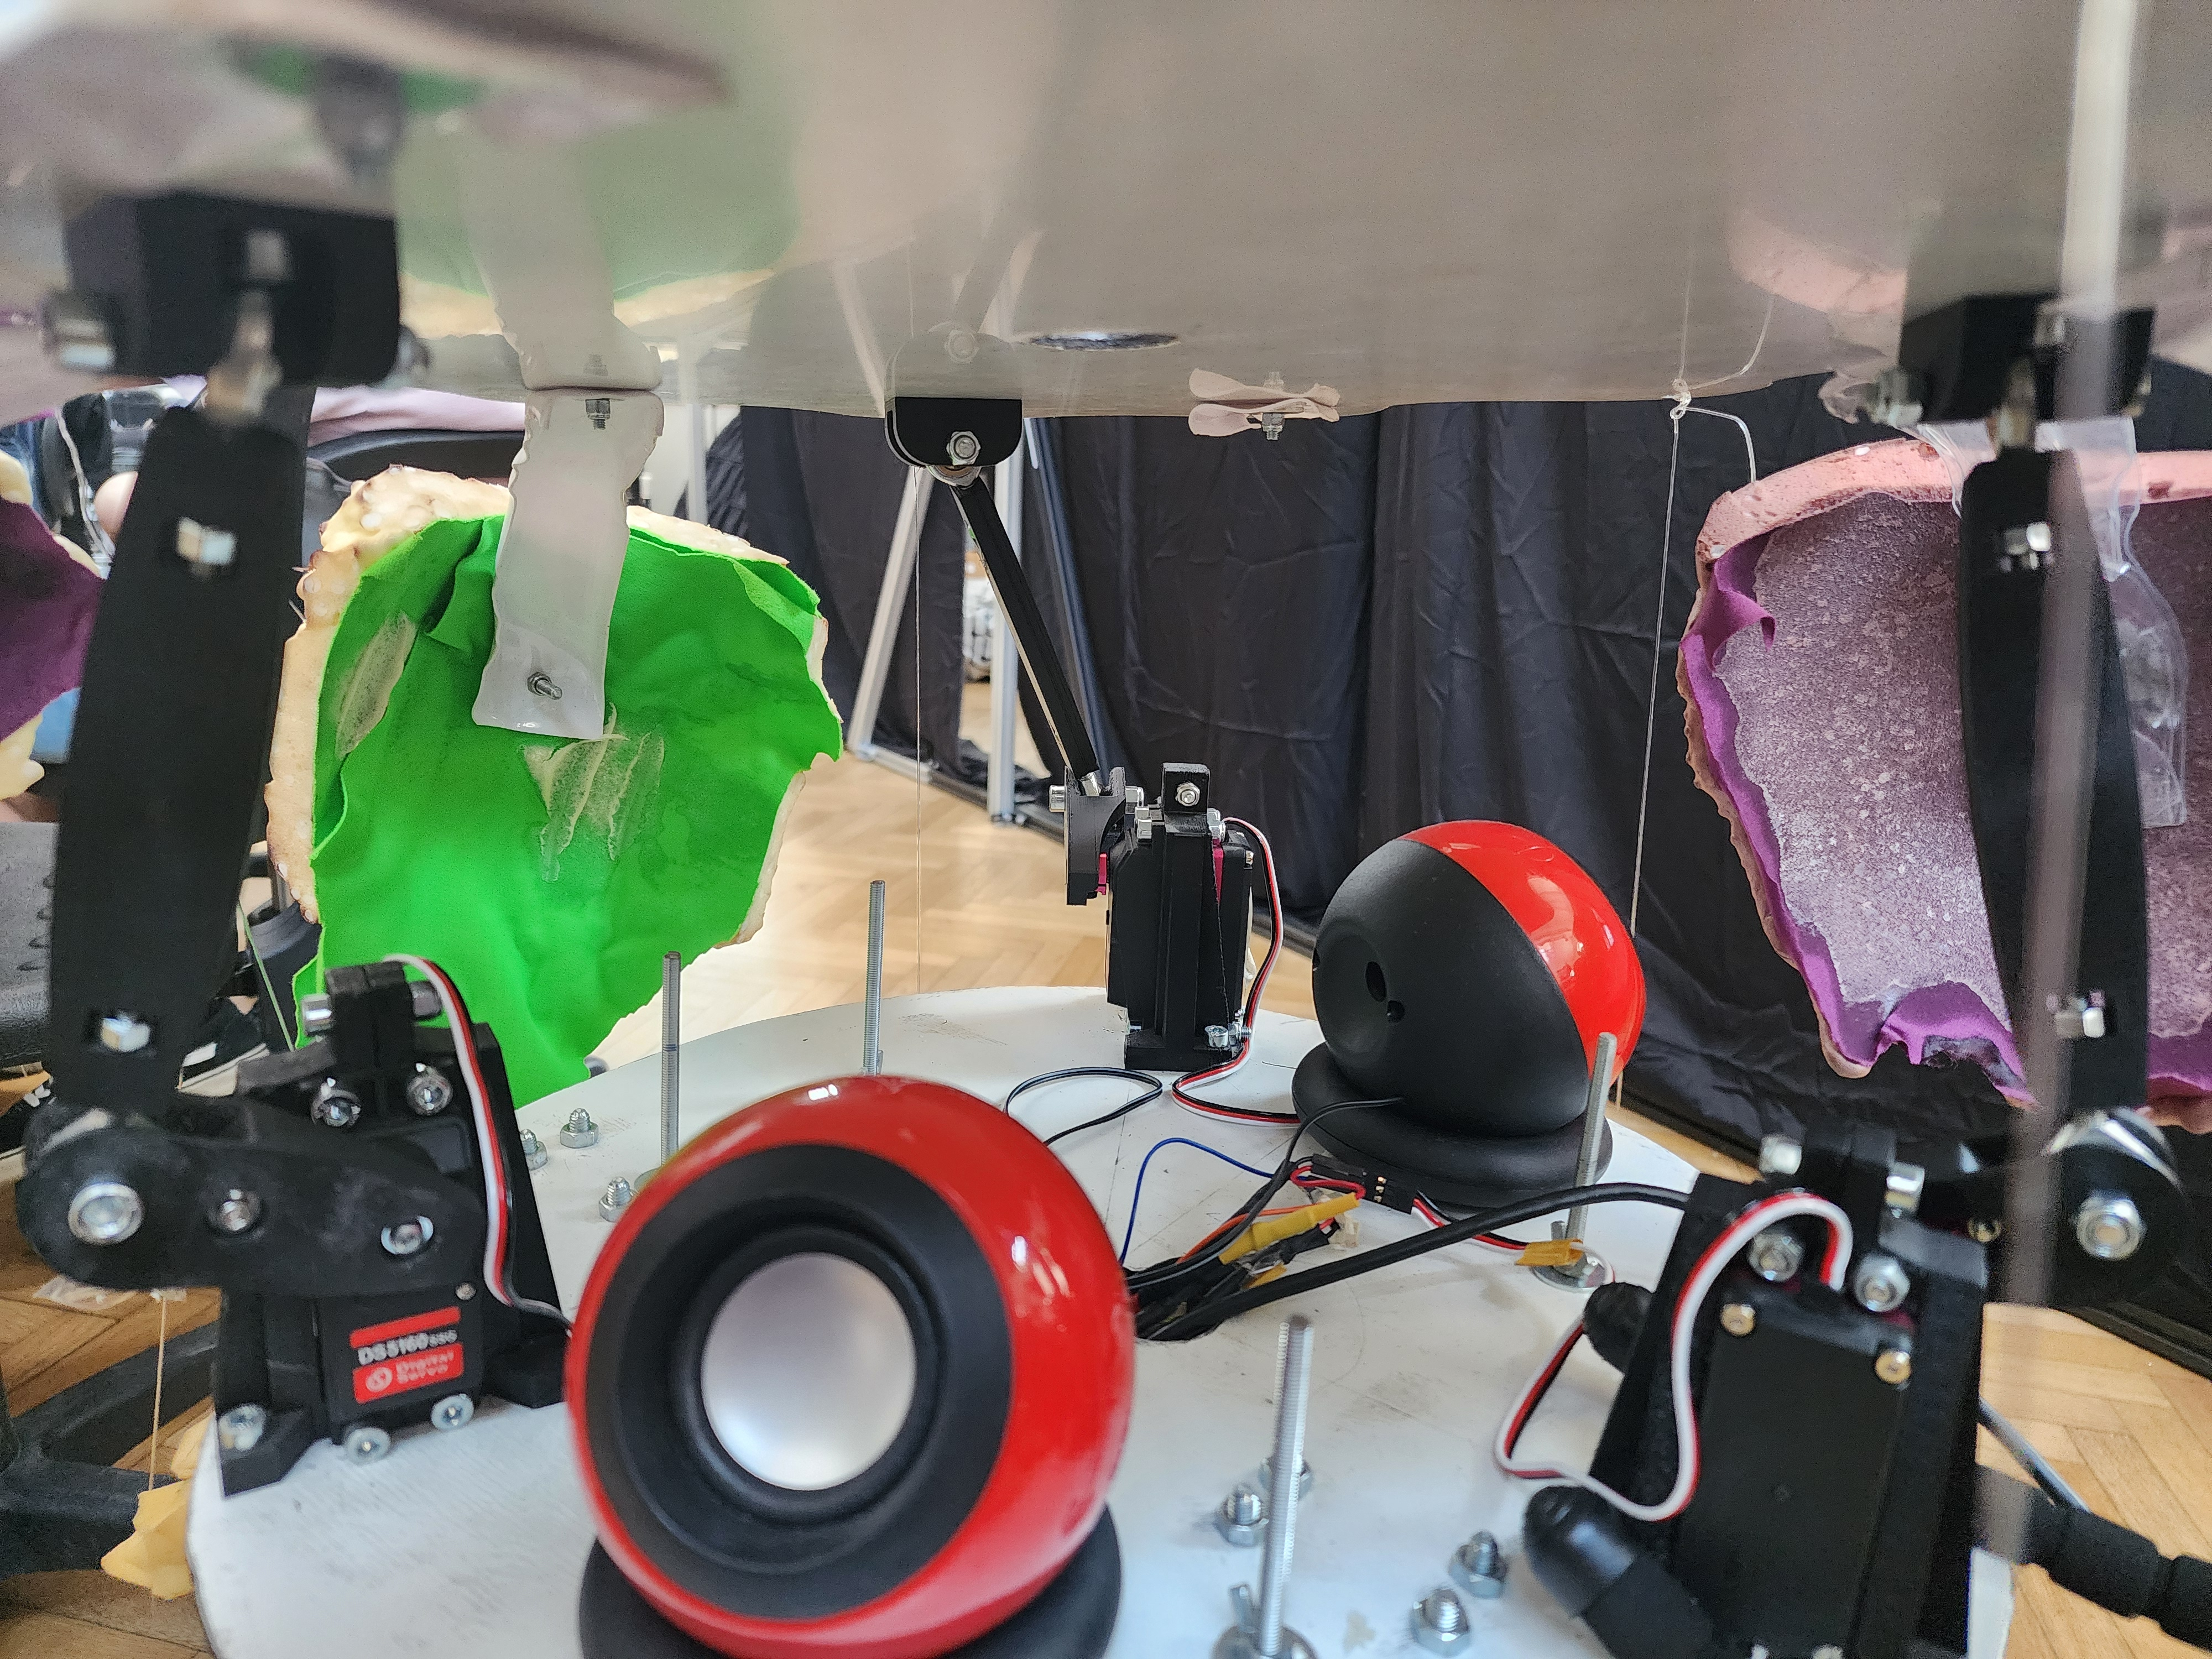
\includegraphics[width=\textwidth]{Images/NewHeadDoubleJoint (2).jpg}
        \caption{Head Arm with Rod Ends (Sway to left)}
        \label{fig:head_arm_rod_end_left}
    \end{minipage}
\end{figure}

Structural strength analysis demonstrates significant improvement in mechanical robustness and load-bearing capability while accepting reduced precision during stationary periods due to joint flexibility. The trade-off provides enhanced durability and operational reliability for social robot applications.

Load capacity testing validates the enhanced design's capability to handle operational loads without component failure or excessive wear. Longevity testing demonstrates sustained performance under extended operational scenarios typical of social robot research applications, though some plastic degradation becomes visible over extended periods while maintaining functional operation.

\subsection{Hybrid Construction Approach}

The final implementation combines 3D printed structural components with metal heim joints to achieve optimal balance between cost, performance, and maintainability.

\subsubsection{Material Selection and Integration}

The hybrid approach utilizes 3D printed PLA components for structural framework elements where weight and cost optimization provide system benefits. Metal heim joints provide superior performance at critical articulation points where durability and precision requirements exceed plastic capabilities.

Integration methodology ensures proper mechanical connection between printed and metal components through threaded interfaces and proper mechanical attachment techniques. Interface design accommodates thermal expansion differences and provides secure long-term connection.

Cost optimization through selective material usage maintains reasonable component costs while providing enhanced performance where critical to system operation. The approach enables high-performance characteristics without excessive cost impact on the overall system.

\section{Camera Integration and Mounting Solutions}

The camera integration system addresses the unique challenges of mounting sophisticated sensing equipment within Tino's soft fabric structure while maintaining the robot's aesthetic characteristics and operational capabilities, while not putting any focal point in evidence.

\begin{figure}[H]
    \centering
    \includegraphics[width=0.6\textwidth, angle=-90]{Images/TripodOnHeadCamera.jpg}
    \caption{Oak-D Pro Camera Mounted on Tripod System}
    \label{fig:tripod_camera_mount}
\end{figure}

\subsection{Mounting System Design and Mechanical Integration}

The camera mounting system provides stable support for the Oak-D Pro camera while integrating with Tino's existing Stewart platform head mechanism and fabric covering system.

\subsubsection{Tripod-Based Support System Development}

The tripod mounting system utilizes simple brackets to create a fixed and stable camera support that eliminates the flexibility and vibration issues encountered with the original Raspberry Pi camera mount. Bracket design prioritizes rigidity while maintaining compatibility with the existing servo head structure.

Mechanical stability analysis demonstrates significant improvement in camera positioning stability compared to the flexible original mount that exhibited excessive movement during robot operation. Static deflection testing validates adequate stiffness for high-quality image acquisition during movement.

The camera mounting system operates independently from the Stewart platform head mechanism, providing dedicated stable positioning for the Oak-D Pro camera without mechanical coupling to head movements. This independent mounting ensures camera stability regardless of head articulation.

\begin{figure}[H]
    \centering
    \begin{minipage}{0.45\textwidth}
        \centering
        \includegraphics[width=\textwidth, angle=-90]{Images/TripodOnHeadCamera (3).jpg}
        \caption{Oak-D Pro Camera Mounted on Tripod System (Side View)}
        \label{fig:tripod_camera_mount_side}
    \end{minipage}
    \hfill
    \begin{minipage}{0.45\textwidth}
        \centering
        \includegraphics[width=\textwidth]{Images/TripodOnHeadCamera (2).jpg}
        \caption{Oak-D Pro Camera Mounted on Tripod System (Top View)}
        \label{fig:tripod_camera_mount_top}
    \end{minipage}
\end{figure}

\subsubsection{Structural Compatibility and Integration Challenges}

The mounting system accommodates the existing servo head geometry while providing secure attachment points for the Oak-D Pro camera. Geometric constraints required custom bracket design that works within the available space while providing adequate support.

Weight distribution analysis ensures that camera addition does not compromise Stewart platform performance or exceed servo motor capabilities. Camera weight integration maintains head balance characteristics while providing enhanced sensing capabilities.

Mechanical interfaces utilize standard mounting hardware that enables camera removal for maintenance or upgrade without requiring bracket system modification. Modular approach provides flexibility for future system enhancement while maintaining operational reliability.

\subsection{Fabric Integration and Visibility Solutions}

The fabric integration system addresses the fundamental challenge of maintaining camera visibility while preserving Tino's fabric aesthetic and protecting sensitive camera components.
\begin{figure}[H]
    \centering
    \begin{minipage}{0.45\textwidth}
        \centering
        \includegraphics[width=\textwidth]{Images/FirstTryCameraHiding.jpg}
        \caption{Initial Camera Concealment Attempt (Front View)}
        \label{fig:first_try_camera_hiding}
    \end{minipage}
    \hfill
    \begin{minipage}{0.45\textwidth}
        \centering
        \includegraphics[width=\textwidth]{Images/FirstTryCameraHiding (3).jpg}
        \caption{Initial Camera Concealment Attempt (Side View)}
        \label{fig:camera_hiding_mesh}
    \end{minipage}
\end{figure}

\subsubsection{Fabric Modification and Positioning Strategies}

Fabric positioning strategies prevent interference with camera sensing while maintaining the robot's aesthetic integrity. Positioning solutions accommodate fabric movement during robot operation without compromising camera field of view or image quality.

Velcro attachment systems provide secure fabric positioning that prevents fabric drift into camera field of view during operational periods. Attachment point selection utilizes strategic locations that maintain fabric appearance while providing reliable position control.

Testing procedures validate fabric positioning effectiveness under various operational scenarios including head movement, robot locomotion, and extended operational periods. Validation testing ensures consistent camera performance throughout typical social interaction scenarios.

\subsubsection{Camera Protection and Environmental Considerations}

Protection requirements address both physical protection from impact during social interaction and environmental protection from dust and moisture that could compromise camera operation. Protection solutions maintain camera accessibility for maintenance while providing adequate operational protection.

The protective approach balances camera protection needs against heat dissipation requirements and optical performance considerations. Protection system design ensures adequate camera cooling while preventing environmental contamination that could affect image quality.

Integration testing validates protection effectiveness while confirming maintained camera performance under operational conditions. Testing includes thermal performance evaluation and optical quality assessment under various environmental conditions.

\subsection{Camera Shell Development and Implementation}

The camera shell system provides comprehensive protection and fabric integration while maintaining optimal camera performance and heat dissipation characteristics.

\begin{figure}[H]
    \centering
    \includegraphics[height=8cm, angle=-90]{Images/CameraCasingNoMesh.jpg}
    \caption{Camera Casing without Mesh Covering}
    \label{fig:camera_casing_no_mesh}
\end{figure}

\subsubsection{Custom Enclosure Design and Functionality}

The custom shell design provides camera protection while maintaining cooling airflow through strategic ventilation openings that enable heat dissipation without compromising environmental protection. Shell geometry optimizes airflow characteristics while minimizing dust ingress.

\begin{figure}[H]
    \centering
    \begin{minipage}{0.45\textwidth}
        \centering
        \includegraphics[width=0.8\textwidth]{Images/CameraCasingMesh.jpg}
        \caption{Camera Casing with Mesh Covering (No camera)} 
        \label{fig:camera_casing_mesh}
    \end{minipage}
    \hfill
    \begin{minipage}{0.45\textwidth}
        \centering
        \includegraphics[width=0.8\textwidth]{Images/CameraCasingMesh (2).jpg}
        \caption{Camera Casing with Mesh Covering (No camera)}
        \label{fig:camera_casing_mesh_back}
    \end{minipage}
\end{figure}

Attachment integration with the tripod mounting system provides secure shell mounting that enables camera access for maintenance while providing operational protection. Mounting system design enables shell removal without disturbing camera alignment or calibration.

Thermal management considerations ensure adequate heat dissipation during extended operation periods, particularly during high-resolution stereo processing that generates significant thermal loads. Thermal testing validates adequate cooling under maximum operational loads.

\begin{figure}[H]
    \centering
    \begin{minipage}{0.45\textwidth}
        \centering
        \includegraphics[width=\textwidth, angle=-90]{Images/CameraCasingNoMesh (4).jpg}
        \caption{Camera Casing without Mesh Covering (Side View)}
        \label{fig:camera_casing_no_mesh_side}
    \end{minipage}
    \hfill
    \begin{minipage}{0.45\textwidth}
        \centering
        \includegraphics[width=\textwidth, angle=-90]{Images/CameraCasingNoMesh (3).jpg}
        \caption{Camera Casing without Mesh Covering (Top View)}
        \label{fig:camera_casing_no_mesh_top}
    \end{minipage}
\end{figure}

\subsubsection{Velcro Fabric Control System}

The fabric control system utilizes velcro attachments integrated with shell flaps to provide positive fabric positioning control. Flap design provides secure attachment points while maintaining fabric flexibility during robot movement.

Velcro implementation includes both shell-mounted components and fabric-sewn counterparts that provide reliable attachment while enabling fabric removal for maintenance. Attachment strength optimization provides secure positioning without excessive fabric stress.

Field testing validates velcro system effectiveness during extended operational periods including various robot movements and interaction scenarios. Testing confirms reliable fabric positioning without attachment failure or fabric damage.

\subsection{Optical Performance Optimization}

The camera integration system maintains optimal optical performance while addressing the unique challenges of fabric-integrated sensing systems.

\subsubsection{Field of View Protection and Optimization}

Field of view protection strategies ensure consistent camera visibility throughout robot operational ranges while accommodating fabric movement and positioning variations. Protection effectiveness validation includes testing under various lighting conditions and robot orientations.

Mesh covering implementation conceals camera presence from casual observation while maintaining full optical transmission characteristics. Mesh selection balances concealment effectiveness against optical performance impact, ensuring minimal image quality degradation.

Optical testing validates maintained image quality and depth sensing performance through the concealment system. Testing includes calibration verification and performance comparison against uncovered camera operation to ensure minimal performance impact.



\section{Audio System Integration}

The audio system integration enables comprehensive bidirectional communication capabilities for VR integration and enhanced human-robot interaction through carefully designed hardware implementation and dynamic audio processing.

\subsection{Hardware Component Selection and Specifications}

The audio hardware selection prioritizes high-quality bidirectional communication capability while maintaining integration compatibility with Tino's existing system architecture and space constraints.

\subsubsection{iTalk-01 Omnidirectional Microphone Integration}

The iTalk-01 omnidirectional microphone provides 360-degree audio capture capability suitable for social robot interaction scenarios where human positioning relative to the robot varies continuously. Microphone specification analysis demonstrates adequate sensitivity and frequency response for speech capture and environmental audio monitoring.

Mounting considerations address the unique challenges of integrating audio capture equipment within Tino's fabric head structure while maintaining acoustic performance and physical protection. Microphone positioning optimization balances audio quality against mechanical protection and aesthetic integration requirements.

Fabric integration methodology enables microphone mounting through strategic fabric modifications that provide audio access without compromising Tino's visual appearance. Integration techniques utilize fabric properties to provide acoustic coupling while maintaining environmental protection for sensitive electronic components.

\subsubsection{Speaker System Selection and Placement}

The speaker system selection prioritizes clear audio reproduction capability within the geometric and weight constraints of Tino's head assembly. Speaker placement within the servo head maximizes available space utilization while providing optimal acoustic coupling for human interaction scenarios.

Acoustic performance optimization addresses the challenges of speaker operation within a constrained and partially enclosed environment. Speaker mounting utilizes available space within the servo head structure while ensuring adequate acoustic coupling and preventing mechanical interference with head movement systems.

Integration with existing head systems ensures speaker mounting does not interfere with Stewart platform operation, camera mounting, or other head-mounted systems. Geometric optimization provides secure speaker mounting while maintaining system accessibility for maintenance and adjustment.
\begin{figure}[H]
    \centering
    \includegraphics[height=6cm]{Images/SpeakerSetup (2).jpg}
    \caption{Speaker Mounted within Servo Head Structure}
    \label{fig:speaker_mount}
\end{figure}

\subsection{Dynamic Audio Generation and Custom Sound Design}

The audio system implements sophisticated sound generation capabilities that create custom ambient audio specifically designed for Tino's character expression and VR integration requirements.

\subsubsection{No-Face Inspired Audio Algorithm}

The dynamic audio generation utilizes a complex algorithm inspired by the No-Face character from Studio Ghibli films, creating an eerie and mysterious ambient sound that enhances Tino's social presence. The \texttt{noface\_params} system maintains breathing phase control, breath cycle management, and dynamic volume adjustment to create organic, living audio characteristics.

The breathing simulation algorithm implements a state machine with inhale and exhale phases, utilizing sinusoidal wave patterns with randomized duration (2.5-4.0 seconds) and volume variations (0.55-0.75 amplitude range) to create natural breathing rhythm variations. The system maintains continuous audio output while avoiding mechanical repetition through breath parameter randomization.

Multi-tone synthesis combines three base frequencies (110Hz, 146.83Hz, 73.42Hz) with pre-calculated gain values (0.65, 0.45, 0.25) to create rich harmonic content. Filtered breath noise generation utilizes a first-order low-pass filter (coefficient 0.92) applied to random noise, creating organic texture that varies with breathing intensity.

The audio generation operates at 44.1kHz sample rate with 1024-sample chunks, ensuring high-quality audio output while maintaining real-time performance compatibility with other system components including SLAM processing and human detection.

\subsubsection{Real-Time Audio Parameter Control}

The audio control system receives real-time parameters from the VR interface through ROS2 topics, enabling dynamic audio modification based on user interaction and robot state. The \texttt{vr\_audio\_callback} function processes \texttt{Float32MultiArray} messages containing volume (0-255 range) and orientation (-1.0 to 1.0 range) control values.

Volume control implementation applies logarithmic scaling to provide natural perceived loudness variations while maintaining system audio output limits. The volume parameter directly scales the final audio amplitude, enabling seamless integration with VR-controlled audio levels based on proximity and interaction intensity.

Orientation-based parameter modulation enables frequency shifting and audio characteristic changes based on spatial positioning. The orientation parameter influences base frequency modulation (±20\% frequency variation) and breathing pattern intensity, creating spatial audio awareness that enhances immersive VR interaction.

\subsection{Stereo Speaker Configuration and Spatial Audio Processing}

The stereo speaker system provides sophisticated spatial audio capabilities through advanced panning algorithms and stereo field manipulation optimized for social robot interaction scenarios.

\subsubsection{Enhanced Stereo Panning Implementation}

The stereo panning system implements aggressive channel separation techniques that create dramatic spatial audio effects controlled by VR input orientation values. The panning algorithm utilizes non-linear curves with exponential falloff characteristics to provide pronounced left-right audio separation that enhances directional audio expression.

Channel separation calculations apply quadratic intensity scaling where \texttt{pan\_intensity = min(1.0, abs(orientation) * 1.5)} creates exponential panning response curves. Right-side dominance utilizes \texttt{left\_vol = volume\_scale * (1.0 - (orientation\_effect * 1.1 + pan\_intensity\^2 * 0.5))} while left-side dominance applies equivalent mirrored calculations for balanced spatial control.

Channel boost implementation provides 30\% amplitude enhancement on the dominant channel (\texttt{right\_vol = volume\_scale * (1.0 + orientation\_effect * 0.3)}) while applying aggressive attenuation up to 95\% on the opposite channel. This creates pronounced stereo separation that maintains 5\% minimum volume to prevent complete channel silence.

The panning system maintains real-time responsiveness with orientation updates processed at audio sample rate, enabling smooth spatial transitions that follow VR user head movements without audible artifacts or discontinuities.

\subsubsection{Audio Expression and Robot Personality Integration}

The stereo audio system enhances Tino's expressive capabilities by correlating spatial audio characteristics with robot emotional states and interaction contexts. Spatial audio positioning creates directional personality expression where left-right audio bias suggests attention direction and emotional focus.

Breathing pattern modulation integrates with stereo positioning to create complex audio landscapes where breath intensity, frequency content, and spatial positioning combine to express robot internal states. The system maintains acoustic coherence while providing rich expressive variation through multi-dimensional audio parameter control.

VR integration enables precise control over robot audio personality through real-time parameter adjustment, allowing users to influence robot audio expression through spatial positioning, proximity, and interaction intensity. This creates responsive audio feedback that enhances social presence and interaction naturalness.

\section{YOLOv11 Pose Detection Implementation with TensorRT Optimization}

The YOLOv11 pose detection system provides real-time human skeleton tracking capabilities optimized for the NVIDIA Orin Nano platform through advanced TensorRT acceleration and efficient model deployment strategies.

\subsection{YOLOv11 Architecture Selection and Model Optimization}

The YOLOv11 architecture selection prioritizes the balance between detection accuracy and computational efficiency required for real-time embedded operation on the Orin Nano platform.

\subsubsection{YOLOv11n-Pose Model Selection}

The \texttt{yolo11n-pose.pt} model provides optimal performance characteristics for the Orin Nano's computational constraints while maintaining adequate accuracy for social robot interaction requirements. The nano variant (11n) utilizes a streamlined architecture with reduced parameter count compared to larger YOLO variants, enabling real-time inference on embedded hardware.

Model architecture analysis demonstrates the YOLOv11n-pose network's capability to detect multiple humans simultaneously within the camera's field of view while maintaining frame rates suitable for interactive applications. The model's optimized backbone reduces computational overhead while preserving essential feature detection capabilities for robust human pose estimation.

Pre-trained model utilization eliminates extensive training requirements by leveraging weights trained on large-scale pose estimation datasets. The pre-trained approach provides immediate deployment capability while ensuring robust performance across diverse human poses and environmental conditions typical of social robot applications.

\subsubsection{Model Format Conversion Pipeline}

The model optimization pipeline transforms the original PyTorch format through multiple conversion stages to achieve maximum performance on the target hardware. The conversion process begins with the native \texttt{.pt} PyTorch format and progresses through ONNX and TensorRT formats for optimal deployment.

ONNX format conversion (\texttt{.onnx}) provides cross-platform compatibility and serves as an intermediate representation that enables hardware-specific optimizations. The ONNX conversion maintains model accuracy while enabling subsequent optimization passes that target the Orin Nano's specific GPU architecture.

TensorRT engine generation (\texttt{.engine}) represents the final optimization stage, creating hardware-specific inference engines that maximize GPU utilization on the Orin Nano platform. The TensorRT optimization process includes layer fusion, precision calibration, and memory access optimization that significantly improve inference performance compared to standard deployment methods.

\subsection{TensorRT Engine Optimization Process}

The TensorRT optimization process generates highly efficient inference engines specifically optimized for the Orin Nano's GPU architecture and memory hierarchy.

\subsubsection{Engine Generation and Hardware Optimization}

TensorRT engine generation utilizes the Orin Nano's specific GPU capabilities to optimize network execution through layer fusion, kernel optimization, and memory access pattern optimization. The process analyzes the YOLOv11n-pose network structure and generates optimized CUDA kernels that maximize throughput while minimizing memory bandwidth requirements.

Precision optimization techniques evaluate the network's sensitivity to reduced precision arithmetic, enabling mixed-precision computation that balances accuracy against performance. The optimization process may utilize INT8 quantization where appropriate while maintaining FP16 or FP32 precision for critical network layers that require higher numerical accuracy.

Memory allocation strategies optimize GPU memory usage patterns to prevent memory fragmentation and minimize allocation overhead during inference operations. The TensorRT engine pre-allocates memory buffers and optimizes data transfer patterns between CPU and GPU memory to minimize inference latency.

\subsubsection{Performance Profiling and Validation}

Engine performance validation ensures that TensorRT optimizations maintain pose detection accuracy while achieving target inference rates. Performance profiling includes accuracy benchmarking against the original PyTorch model to verify that optimization processes do not compromise detection quality.

Throughput analysis measures inference performance under various loading conditions including single and multi-person detection scenarios. Performance metrics include inference latency, GPU utilization, and memory bandwidth utilization that validate the engine's suitability for real-time social robot applications.

Thermal analysis ensures that sustained inference operations remain within the Orin Nano's thermal limits during extended operation periods. Thermal validation includes continuous operation testing under maximum computational loads to ensure system stability and reliability.

\subsection{ROS2 Node Architecture and Integration}

The pose detection system integrates seamlessly with Tino's ROS2 architecture through a dedicated node that manages camera input, inference execution, and result publication.

\subsubsection{Camera Topic Subscription and Data Flow}

The \texttt{pose\_detection\_node.py} subscribes to Oak-D Pro camera topics including \texttt{/right/image\_rect} for monocular RGB input and \texttt{/stereo/depth} for corresponding depth information required for 3D coordinate calculation. The node implements efficient message handling with \texttt{CvBridge} conversion from ROS2 image messages to OpenCV format suitable for YOLO processing.

Image preprocessing includes monocular to BGR conversion for YOLO compatibility, since the implementation uses the right camera feed converted from mono8 to BGR format. The preprocessing pipeline utilizes CPU-based OpenCV operations for format conversion while maintaining real-time performance through efficient memory management.

Synchronization mechanisms maintain temporal alignment between RGB and depth image streams through callback-based processing that ensures corresponding depth information is available for each processed RGB frame. The implementation uses a latest-frame approach where \texttt{latest\_image} and \texttt{latest\_depth\_image} are synchronized for pose detection processing.

\subsubsection{Inference Execution and Result Processing}

TensorRT inference execution utilizes the pre-converted \texttt{yolo11n-pose.engine} model loaded from the package resource directory through \texttt{YOLO (model\_path)} initialization. The inference pipeline processes BGR images directly with configurable confidence thresholding (default 0.5) and \texttt{verbose=False} parameter to suppress detection logging output.

Result post-processing extracts pose keypoints, confidence scores, and bounding box information from the \texttt{results[0]} object returned by YOLO inference. Post-processing operations include confidence-based filtering, closest person selection based on depth measurements, and coordinate extraction from the \texttt{results[0].boxes} and \texttt{results[0].keypoints} attributes.

Error handling implements comprehensive exception management with detailed logging at configurable levels (INFO, DEBUG, ERROR) and graceful degradation when model loading fails or inference encounters errors. The system maintains operational continuity through try-catch blocks around critical processing sections.

\section{Stereo Depth Integration for 3D Human Positioning}

The stereo depth integration system combines 2D pose detection results with Oak-D Pro depth information to provide accurate 3D human positioning capabilities essential for spatial awareness and interaction planning.

\subsection{Oak-D Pro Depth Data Utilization}

The Oak-D Pro camera system provides synchronized stereo depth information that enables precise 3D coordinate calculation for detected human pose keypoints.

\subsubsection{Stereo Depth Acquisition and Processing}

The Oak-D Pro stereo camera system generates depth maps through stereo vision algorithms that calculate depth values for each pixel in the synchronized color image. Depth data accuracy depends on stereo baseline, camera calibration quality, and environmental factors including lighting conditions and surface textures.

Depth value extraction utilizes a median-based approach with a 9x9 pixel window around keypoint locations to obtain robust depth measurements. The \texttt{get\_depth\_at\_point} function implements outlier filtering by calculating median and standard deviation, then filtering values more than 2 standard deviations from the median to ensure reliable depth extraction.

Depth data validation implements comprehensive quality filtering including zero-value rejection, outlier detection based on statistical analysis, and temporal smoothing over a configurable window size (default 3 frames). The validation process uses median filtering within pixel windows and consistency checks against reference depth values to maintain measurement reliability.

For person detection, the system uses \texttt{get\_median\_depth} function that extracts depth from a central region of the bounding box with configurable padding (25\% by default), providing more stable depth measurements than single-pixel sampling while avoiding background contamination.

\subsubsection{Coordinate System Transformation}

Camera frame to robot coordinate transformation converts 3D keypoint coordinates using the \texttt{calculate\_3d\_position} function that utilizes camera intrinsic parameters from \texttt{camera\_info.k} array. The transformation extracts focal lengths \texttt{fx}, \texttt{fy} and principal point coordinates \texttt{cx}, \texttt{cy} from the camera calibration matrix.

Intrinsic parameter utilization includes automatic unit conversion detection where depth values greater than 100 are converted from millimeters to meters, followed by depth calibration correction using configurable \texttt{depth\_scale\_factor} (default 0.575) and \texttt{depth\_offset} parameters derived from empirical calibration measurements.

3D coordinate calculation applies the standard pinhole camera model: \texttt{x\_3d = (x - cx) * z / fx} and \texttt{y\_3d = (y - cy) * z / fy}, where corrected depth \texttt{z = z * depth\_scale\_factor + depth\_offset} accounts for systematic depth measurement biases in the Oak-D Pro stereo system.

\subsection{3D Skeleton Generation and Validation}

The 3D skeleton generation process combines 2D keypoint detections with corresponding depth values to create complete 3D human pose representations.

\subsubsection{Keypoint Depth Association}

Depth value assignment utilizes the 2D keypoint pixel coordinates to extract corresponding depth measurements from the stereo depth map. The assignment process includes validation to ensure depth measurements correspond to human body parts rather than background objects.

Depth consistency validation utilizes a sophisticated temporal smoothing system where individual keypoint depths are validated against a reference depth calculated as the median of all valid keypoint depths. The \texttt{process\_skeleton} function implements outlier rejection where keypoint depths deviating more than the configurable \texttt{depth\_outlier\_threshold} (default 30\%) from the reference are replaced with the temporal median depth from a smoothing window.

Missing depth handling addresses invalid keypoint scenarios through the reference depth fallback system. When keypoint coordinates are marked as invalid ($x \leq 0$ or $y \leq 0$) or depth extraction fails, the system utilizes the temporally smoothed reference depth calculated from all valid keypoints in the current frame, ensuring skeleton completeness even with partial occlusion.

The temporal smoothing implementation maintains a \texttt{skeleton\_depth\_history} list with configurable window size (default 3 frames) that stores reference depths for median filtering over time, providing stable depth values that reduce measurement jitter while maintaining responsiveness to actual depth changes.

\subsection{Real-time Processing and Performance Optimization}

The 3D positioning system maintains real-time performance while processing high-resolution depth data and performing complex coordinate transformations.



\section{Real-time Skeleton Tracking with 17 Key Body Joints}

The skeleton tracking system processes YOLOv11 pose detection results to extract and organize 17 standard COCO keypoints into structured human pose representations suitable for social robot interaction analysis.

\subsection{COCO Keypoint Framework Implementation}

The COCO keypoint framework provides a standardized representation for human pose detection that ensures compatibility with established computer vision tools and datasets.

\subsubsection{17-Keypoint Detection Schema}

The YOLOv11 pose detection system identifies 17 key body joints following the COCO pose estimation standard: nose (0), left eye (1), right eye (2), left ear (3), right ear (4), left shoulder (5), right shoulder (6), left elbow (7), right elbow (8), left wrist (9), right wrist (10), left hip (11), right hip (12), left knee (13), right knee (14), left ankle (15), and right ankle (16).

Joint indexing follows the established COCO convention ensuring compatibility with existing pose analysis tools and datasets. The consistent indexing scheme enables straightforward integration with pose analysis algorithms and facilitates comparison with other human pose detection systems.

Keypoint connectivity defines the skeletal structure through predefined joint relationships that represent human anatomical connections. The connectivity graph includes head structure (nose-eyes-ears), torso connections (shoulders-hips), and limb chains (shoulder-elbow-wrist, hip-knee-ankle) that enable skeletal validation and pose completeness assessment.

\subsubsection{Confidence Scoring and Quality Assessment}

Confidence score extraction provides reliability metrics for each detected keypoint, enabling quality-based filtering and uncertainty quantification. Confidence values range from 0.0 (undetected) to 1.0 (high confidence) and indicate the detection algorithm's certainty in keypoint localization accuracy.

Quality thresholding implements confidence-based filtering that excludes low-confidence detections from downstream processing. Threshold values balance detection completeness against accuracy requirements, with typical thresholds ranging from 0.3 to 0.7 depending on application requirements and environmental conditions.

Multi-person confidence handling manages confidence scores when multiple humans are detected simultaneously. The system maintains separate confidence profiles for each detected person while implementing consistency checks that ensure skeletal coherence within individual pose detections.

\subsection{Data Processing Pipeline and Skeleton Organization}

The data processing pipeline transforms raw YOLOv11 output into structured skeleton representations suitable for real-time robot applications.

\subsubsection{Keypoint Coordinate Extraction}

Raw network output processing extracts keypoint coordinates and confidence scores from YOLOv11 inference results. The extraction process handles variable-length outputs that accommodate different numbers of detected humans while maintaining consistent data structures for downstream processing.

Coordinate normalization converts pixel coordinates to standardized coordinate systems that enable consistent processing regardless of camera resolution or field of view variations. Normalization includes scaling, translation, and coordinate system alignment that simplifies subsequent geometric calculations.

\subsubsection{Skeleton Structure Validation}

Geometric consistency validation implements anatomical constraints that verify reasonable joint relationships within detected skeletons. Validation includes bone length checks, joint angle limitations, and bilateral symmetry assessments that identify and filter implausible pose detections.

Temporal consistency analysis compares consecutive pose detections to identify and smooth measurement noise while detecting rapid pose changes that indicate genuine human motion. Temporal filtering balances noise reduction against motion tracking accuracy to maintain responsive pose tracking.

Completeness assessment evaluates skeleton quality based on the number and distribution of successfully detected keypoints. Assessment criteria include minimum keypoint requirements, critical joint detection (head, torso, limbs), and pose coverage metrics that indicate skeleton suitability for specific applications.

\subsection{ROS2 Message Publishing and Data Distribution}

The skeleton tracking system publishes pose data through ROS2 topics enabling integration with other robot systems and applications.

\subsubsection{Custom Message Structure Design}

ROS2 message design implements multiple specialized publishers for different data requirements: \texttt{/pose\_detection/image\_raw} for annotated detection images, \texttt{/human\_position} for smoothed human position using \texttt{PoseStamped} messages, \texttt{/human\_skeleton} for 3D skeleton visualization using \texttt{MarkerArray}, and \texttt{/human\_skeleton\_poses} for programmatic access to joint coordinates using \texttt{PoseArray} messages.

Multi-person message handling focuses on closest person selection based on depth measurements, where the system identifies the person with minimum depth value and processes only that individual's skeleton data. This approach reduces computational overhead while ensuring consistent tracking of the most relevant human for interaction applications.

Timestamp synchronization utilizes \texttt{self.get\_clock ().now ().to\_msg ()} for all published messages with consistent \texttt{header.frame\_id} set to the configurable camera frame (default: \texttt{oak\_right\_camera\_optical\_frame}), ensuring temporal alignment across all pose-related data streams.

\subsection{Integration with Robot Controller and VR Systems}

Skeleton data integration enables sophisticated human-robot interaction capabilities through real-time pose information distribution to various robot subsystems.

\subsubsection{Robot Controller Integration}

The robot controller subscribes to \texttt{/human\_position} topic for spatial awareness applications where human position data undergoes temporal smoothing through the \texttt{publish\_human\_position} function. This implementation maintains a configurable history buffer (default 5 positions) and publishes averaged coordinates to reduce measurement jitter while maintaining responsiveness to human movement.

Pose-based behavior triggers can utilize the multiple data streams including raw skeleton data from \texttt{/human\_skeleton\_poses} for detailed joint analysis, smoothed position data from \texttt{/human\_position} for proximity detection, and visual markers from \texttt{/human\_skeleton} for debugging and visualization purposes.

Safety monitoring implementation prioritizes closest person detection where the system automatically selects the human with minimum depth measurement for tracking, ensuring safety systems focus on the most immediate interaction partner while maintaining computational efficiency through single-person processing.

\subsubsection{VR Data Recording and Transmission}

VR system integration transmits skeleton data for immersive visualization and interaction analysis applications. Integration includes data formatting for Unity applications and network transmission protocols optimized for VR system requirements.

Data recording capabilities capture complete skeleton tracking sessions for offline analysis and system evaluation. Recording includes synchronized pose data, camera images, and robot state information that enable comprehensive interaction analysis and system performance assessment.

Bandwidth optimization implements data compression and selective transmission strategies that maintain VR system responsiveness while minimizing network overhead. Optimization techniques include keyframe detection, delta encoding, and adaptive quality adjustment based on network conditions and VR application requirements.


\section{VR System Architecture and Unity Communication}

The VR integration system enables immersive remote control of Tino through Unity-based VR environments via a bidirectional UDP communication protocol that maintains real-time responsiveness while providing comprehensive robot state information.

\subsection{VR Interface Node Architecture}

The \texttt{vr\_interface\_node.py} serves as the central communication bridge between Tino's ROS2 ecosystem and Unity VR applications. The node subscribes to robot pose data (\texttt{/vr\_in/robot\_pose}), human skeleton information (\texttt{/vr\_in/human\_skeleton\_poses}), and audio output (\texttt{/vr\_in/audio\_output}), while publishing VR control commands to \texttt{/vr\_out/cmd\_vel} for base movement and \texttt{/vr\_out/head\_cmd} for head articulation.

The multi-threaded architecture utilizes dedicated UDP listener threads with 1-second timeouts for non-blocking message reception while enabling simultaneous outgoing data transmission. Error handling includes automatic VR disconnection detection (3-second timeout) and message ordering counter reset upon reconnection.

\subsection{UDP Communication Protocol}

The protocol implements a three-port architecture for parallel data streams: port 5005 receives 32-byte VR command packets, port 5006 transmits 24-byte robot pose data, and port 5007 streams 208-byte skeleton data containing 17 COCO-format joints.

Incoming command packets contain 3 floats for head control (pitch, pan, tilt), 2 integers for base commands (state 0-3, angular direction -1/0/1), 2 values for audio control (volume 0-255, orientation -1.0 to 1.0), and 1 integer for message ordering. Binary encoding uses \texttt{struct.unpack('fffiiffi', data)} with validation for length verification and parameter range checking.

Outgoing pose packets include message ordering, position coordinates (x, y), orientation quaternion (z, w), and audio volume, optimized for 10Hz transmission rates. Message ordering counters enable detection of lost, duplicate, or out-of-order packets with automatic counter reset during reconnection events.

\section{Atomic Movement System Design and 4-State Control Architecture}

The atomic movement system replaces traditional continuous control with discrete, completion-guaranteed movements ensuring perfect correspondence between VR user intentions and physical robot actions. The unified 4-state framework provides standardized behavior across both leg and base controllers.

\subsection{4-State Control Framework}

\subsubsection{State 0: Idle and Auto-Positioning}

State 0 maintains neutral configurations with intelligent auto-positioning for the leg controller. The system uses absolute encoder feedback to calculate position differences from neutral (0 ticks) and applies appropriate motor commands: 110 RPM forward when negative position, 70 RPM backward when positive, and 90 RPM neutral when within 50 ticks. The base controller implements complete motion cessation with flag reset.

\subsubsection{State 1: Expressive ``Little Push'' Movements}

State 1 implements attention-getting behaviors. The leg controller uses an optimized 3-phase pattern: 50\% forward extension, 5\% pause, 45\% return over 1.2 seconds via the \texttt{vtLittlePush()} function. The base controller executes a 600ms delay, 200ms forward, 200ms backward sequence for directional indication.

\subsubsection{State 2: Timing Synchronization}

State 2 enables coordinated multi-component movements. The leg controller extends to maximum reach using \texttt{vtForwardOnly()} then activates position hold mode with PID control (Kp=2.0, Ki=0.1, Kd=0.5). The base controller implements a 1.5-second timing cycle with command queuing for received case 3 commands.

\subsubsection{State 3: Atomic Movement Execution}

State 3 executes completion-guaranteed operations. The leg controller returns to neutral using home button detection as completion criteria. The base controller provides three movement types: forward (angular=0), right rotation (angular=1), left rotation (angular=-1), each with 1.7-second duration.

\subsection{Implementation Details}

The leg controller maintains absolute position through encoder integration with direction-specific scaling (forward 1.15, backward 0.85) and automatic reset on button press. The base controller uses \texttt{updateBaseMovementByTime()} with millisecond-precision timing and sophisticated locking mechanisms (\texttt{isCase2Locked}) that coordinate execution between components.

\section{Pulse-Based Command System for VR Integration}

The pulse-based command architecture replaces continuous signal transmission with discrete 3-cycle command pulses that automatically return to idle state, guaranteeing that each VR interaction triggers exactly one complete robot movement cycle.

\subsection{Command Pulse Structure}

Each user action generates three identical command cycles followed by automatic return to idle (command 0). Pulse timing uses 40ms intervals between transmissions (120ms total duration) to exceed network latency variations while preventing command accumulation. The 3-cycle repetition ensures reliable delivery across network interruptions with command validation through parameter consistency checking.

VR input processing transforms continuous actions into discrete events through rising-edge triggering on button activation, preventing continuous command generation during extended holds. Input debouncing requires 200ms minimum intervals between commands while encoding current VR state (head orientation) at command initiation time.

\subsection{Gamepad Development Integration}

Gamepad control mirrors VR functionality using discrete button commands: X (state 1), Y (state 2), B (state 3), A (idle). Shoulder buttons enable combined movement testing with simultaneous angular direction commands. The identical pulse generation system ensures development testing accurately represents VR operational behavior.

\subsection{VR Command Processing}

UDP packet processing extracts commands from 32-byte binary structures using \texttt{struct.unpack('fffiiffi', data)} format. Head commands (pitch, pan, tilt) forward directly to robot controllers, while base commands (state 0-3, angular -1/0/1) trigger atomic movement execution. Message ordering uses 32-bit sequence numbers for duplicate detection and lost packet monitoring, with automatic counter reset during VR reconnection events.

\section{Unity-ROS2 Communication Protocol and Message Structures}

The Unity-ROS2 communication protocol implements optimized UDP-based data exchange designed for real-time VR applications with robust reliability and comprehensive monitoring capabilities.

\subsection{Multi-Port UDP Architecture}

The system uses three dedicated ports for parallel data streams: port 5005 (VR commands, 32-byte packets), port 5006 (robot pose, 24-byte packets), and port 5007 (skeleton data, 208-byte packets). This isolation prevents interference while enabling independent optimization for different data types and latency requirements.

Network configuration supports flexible deployment through configurable IP addresses and transmission rates. Default settings target address 192.168.0.201 with pose/skeleton transmission at 10Hz and expected command reception at 25Hz.

\subsection{Message Format Specifications}

Incoming VR commands use a 32-byte binary format: 3 floats (head pitch/pan/tilt), 2 integers (base state 0-3, angular direction -1/0/1), 2 values (audio volume 0-255, orientation -1.0 to 1.0), and 1 integer (message ordering). Binary encoding uses \texttt{struct.unpack('fffiiffi', data)} with comprehensive validation for length, range, and ordering.

Outgoing robot pose packets contain: message ordering, position coordinates (x, y), orientation quaternion (z, w), and audio volume in 24 bytes. Skeleton packets include 51 floats representing 17 COCO joints with default (0,0,0) coordinates for missing joints.

\subsection{Communication Health Monitoring}

The system implements comprehensive monitoring including rate validation against configured targets, connection status tracking with 3-second disconnection timeout, and message ordering validation for duplicate/loss detection. Automatic recovery includes counter reset upon reconnection and detailed diagnostic logging for system maintenance.

\subsection{External Appearance Impact Assessment}

Throughout the comprehensive Tino V2 implementation encompassing ROS2 architecture migration, kinematic base redesign, power system overhaul, Stewart platform improvements, camera integration, and audio system enhancements, the robot's external aesthetic appearance has been deliberately preserved to maintain its distinctive character and proven social interaction capabilities.

The extensive internal modernization—from the fundamental shift to differential drive kinematics and NVIDIA Orin Nano computational platform to the complete redesign of head mechanisms and sensor integration—was strategically executed to operate within Tino's established external form factor. Each upgrade was carefully engineered to enhance technical capabilities while preserving the approachable aesthetic that defines Tino's social robotics effectiveness.

\begin{figure}[H]
    \centering
    \begin{minipage}{0.45\textwidth}
        \centering
        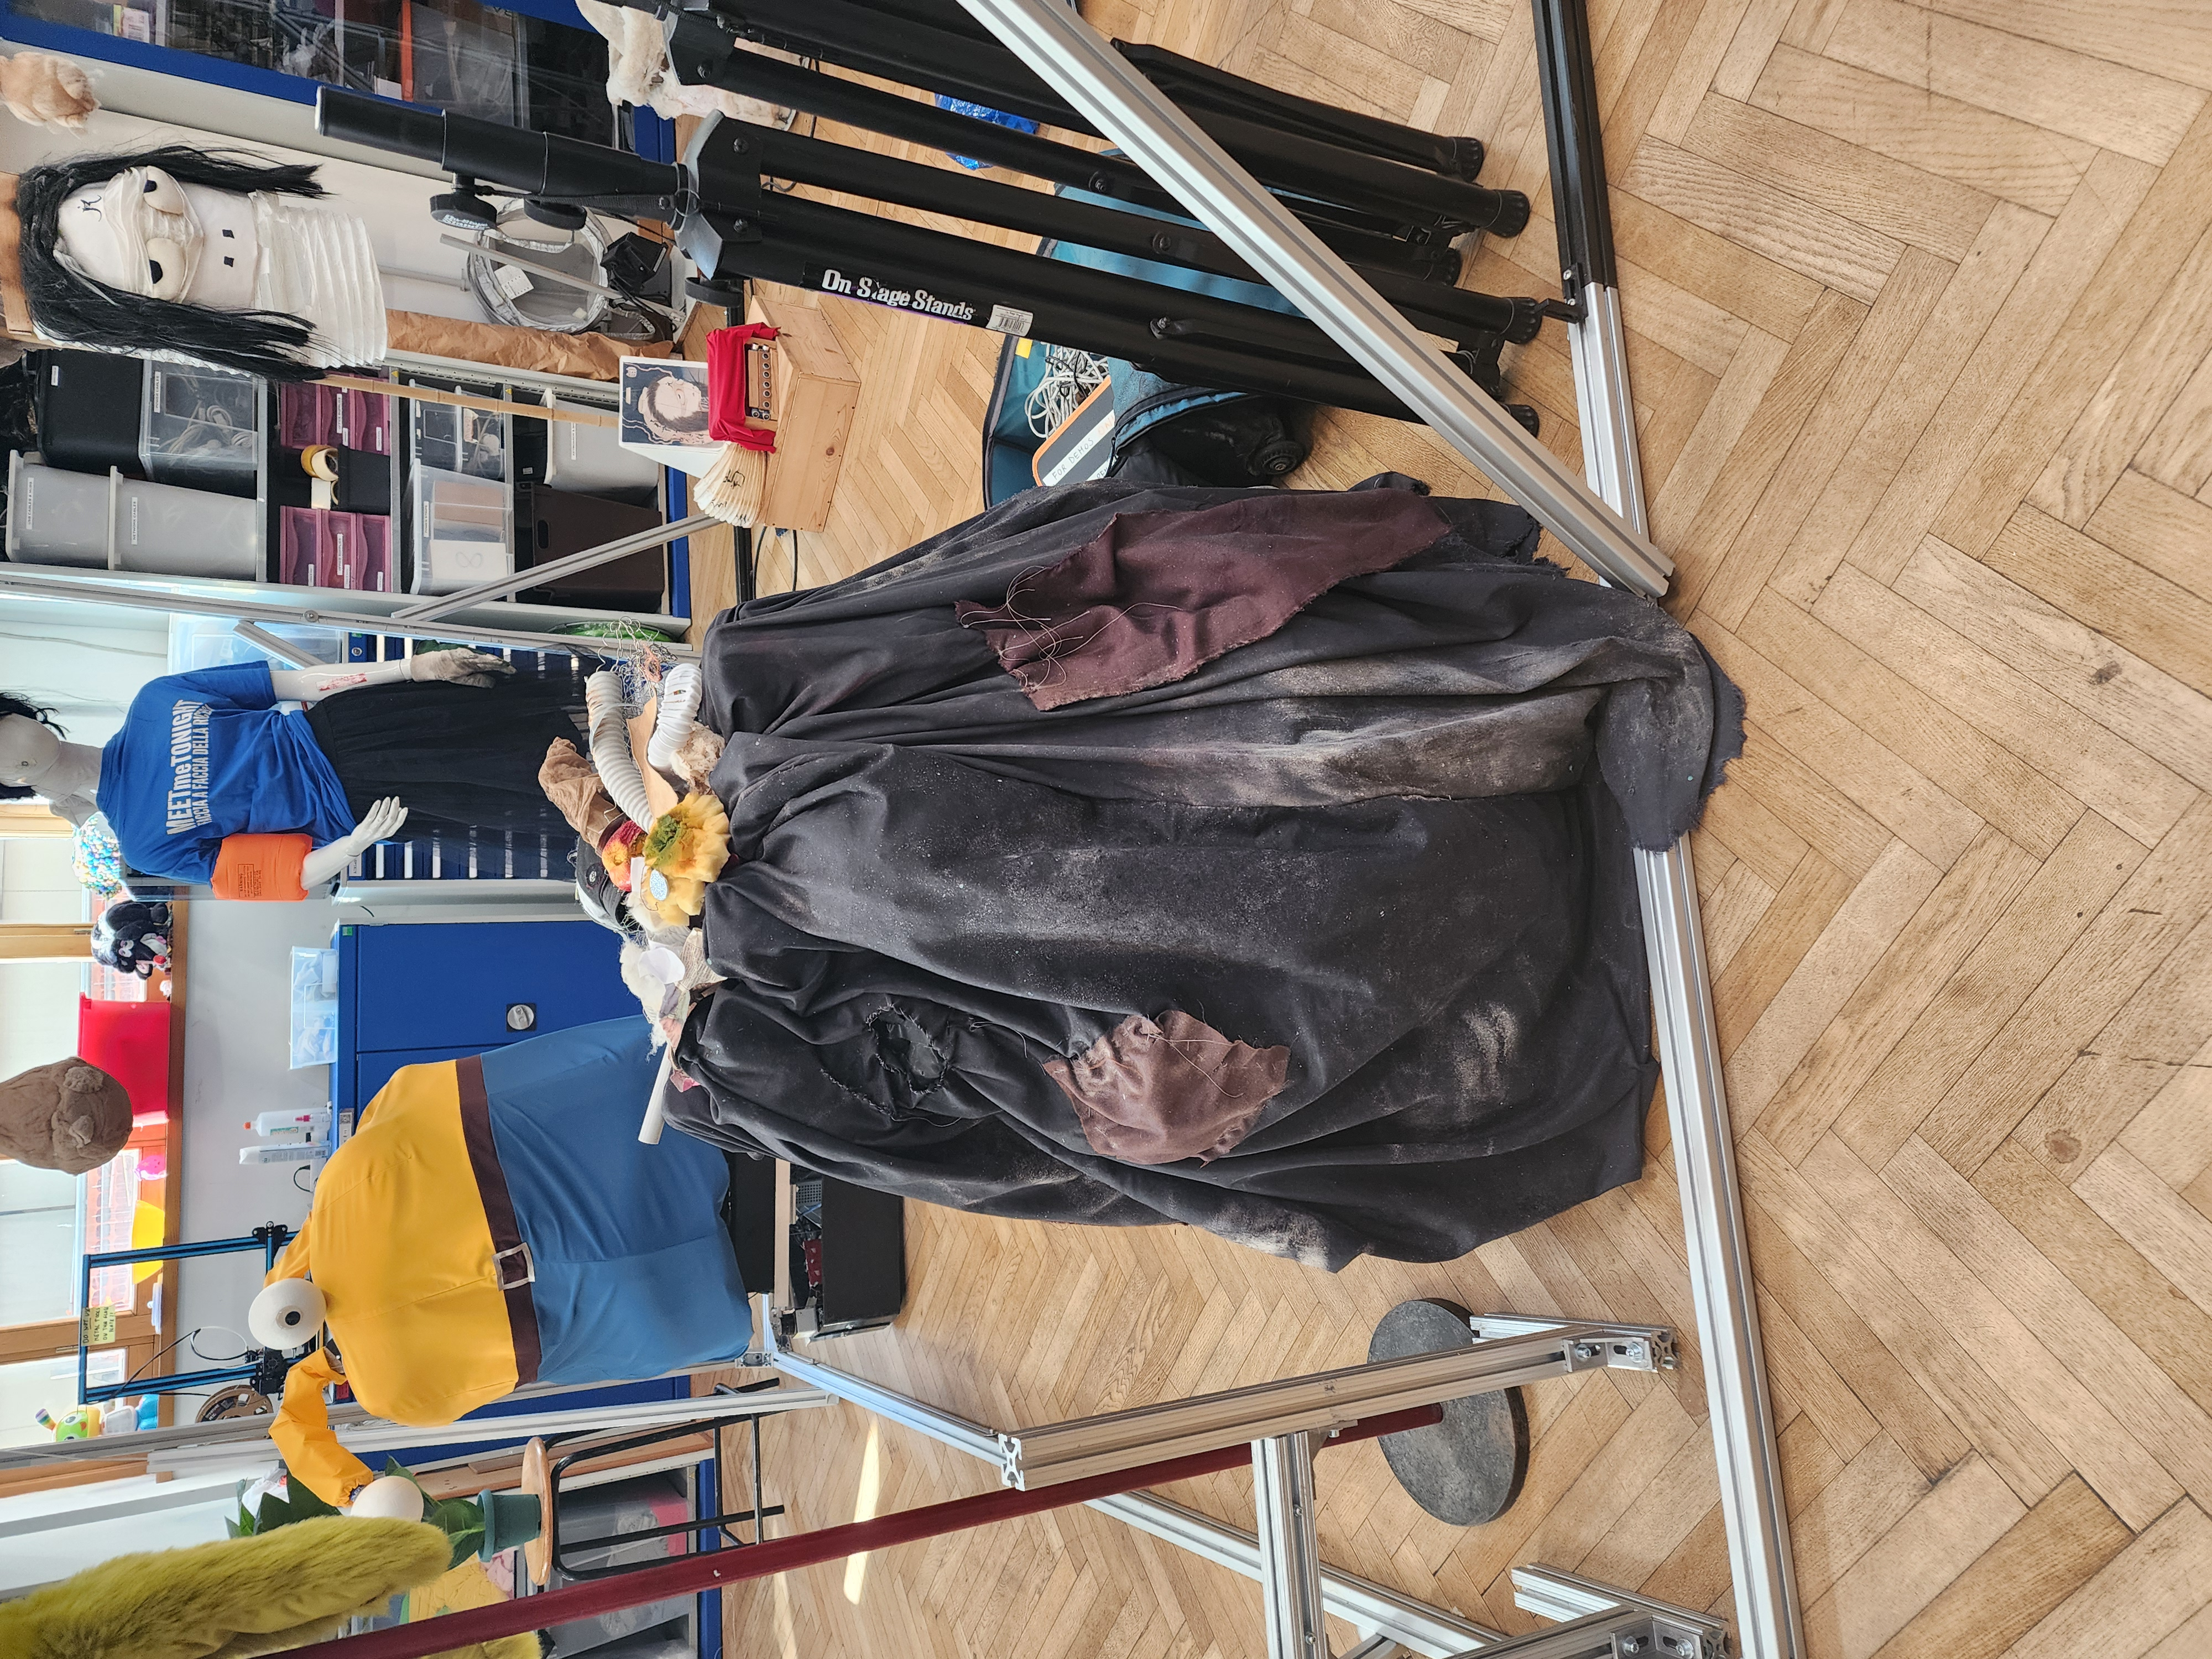
\includegraphics[width=\textwidth, angle=-90]{Images/TinoBefore.jpg}
        \caption{Tino Before V2 Implementation}
        \label{fig:tino_before_upgrade}
    \end{minipage}
    \hfill
    \begin{minipage}{0.45\textwidth}
        \centering
        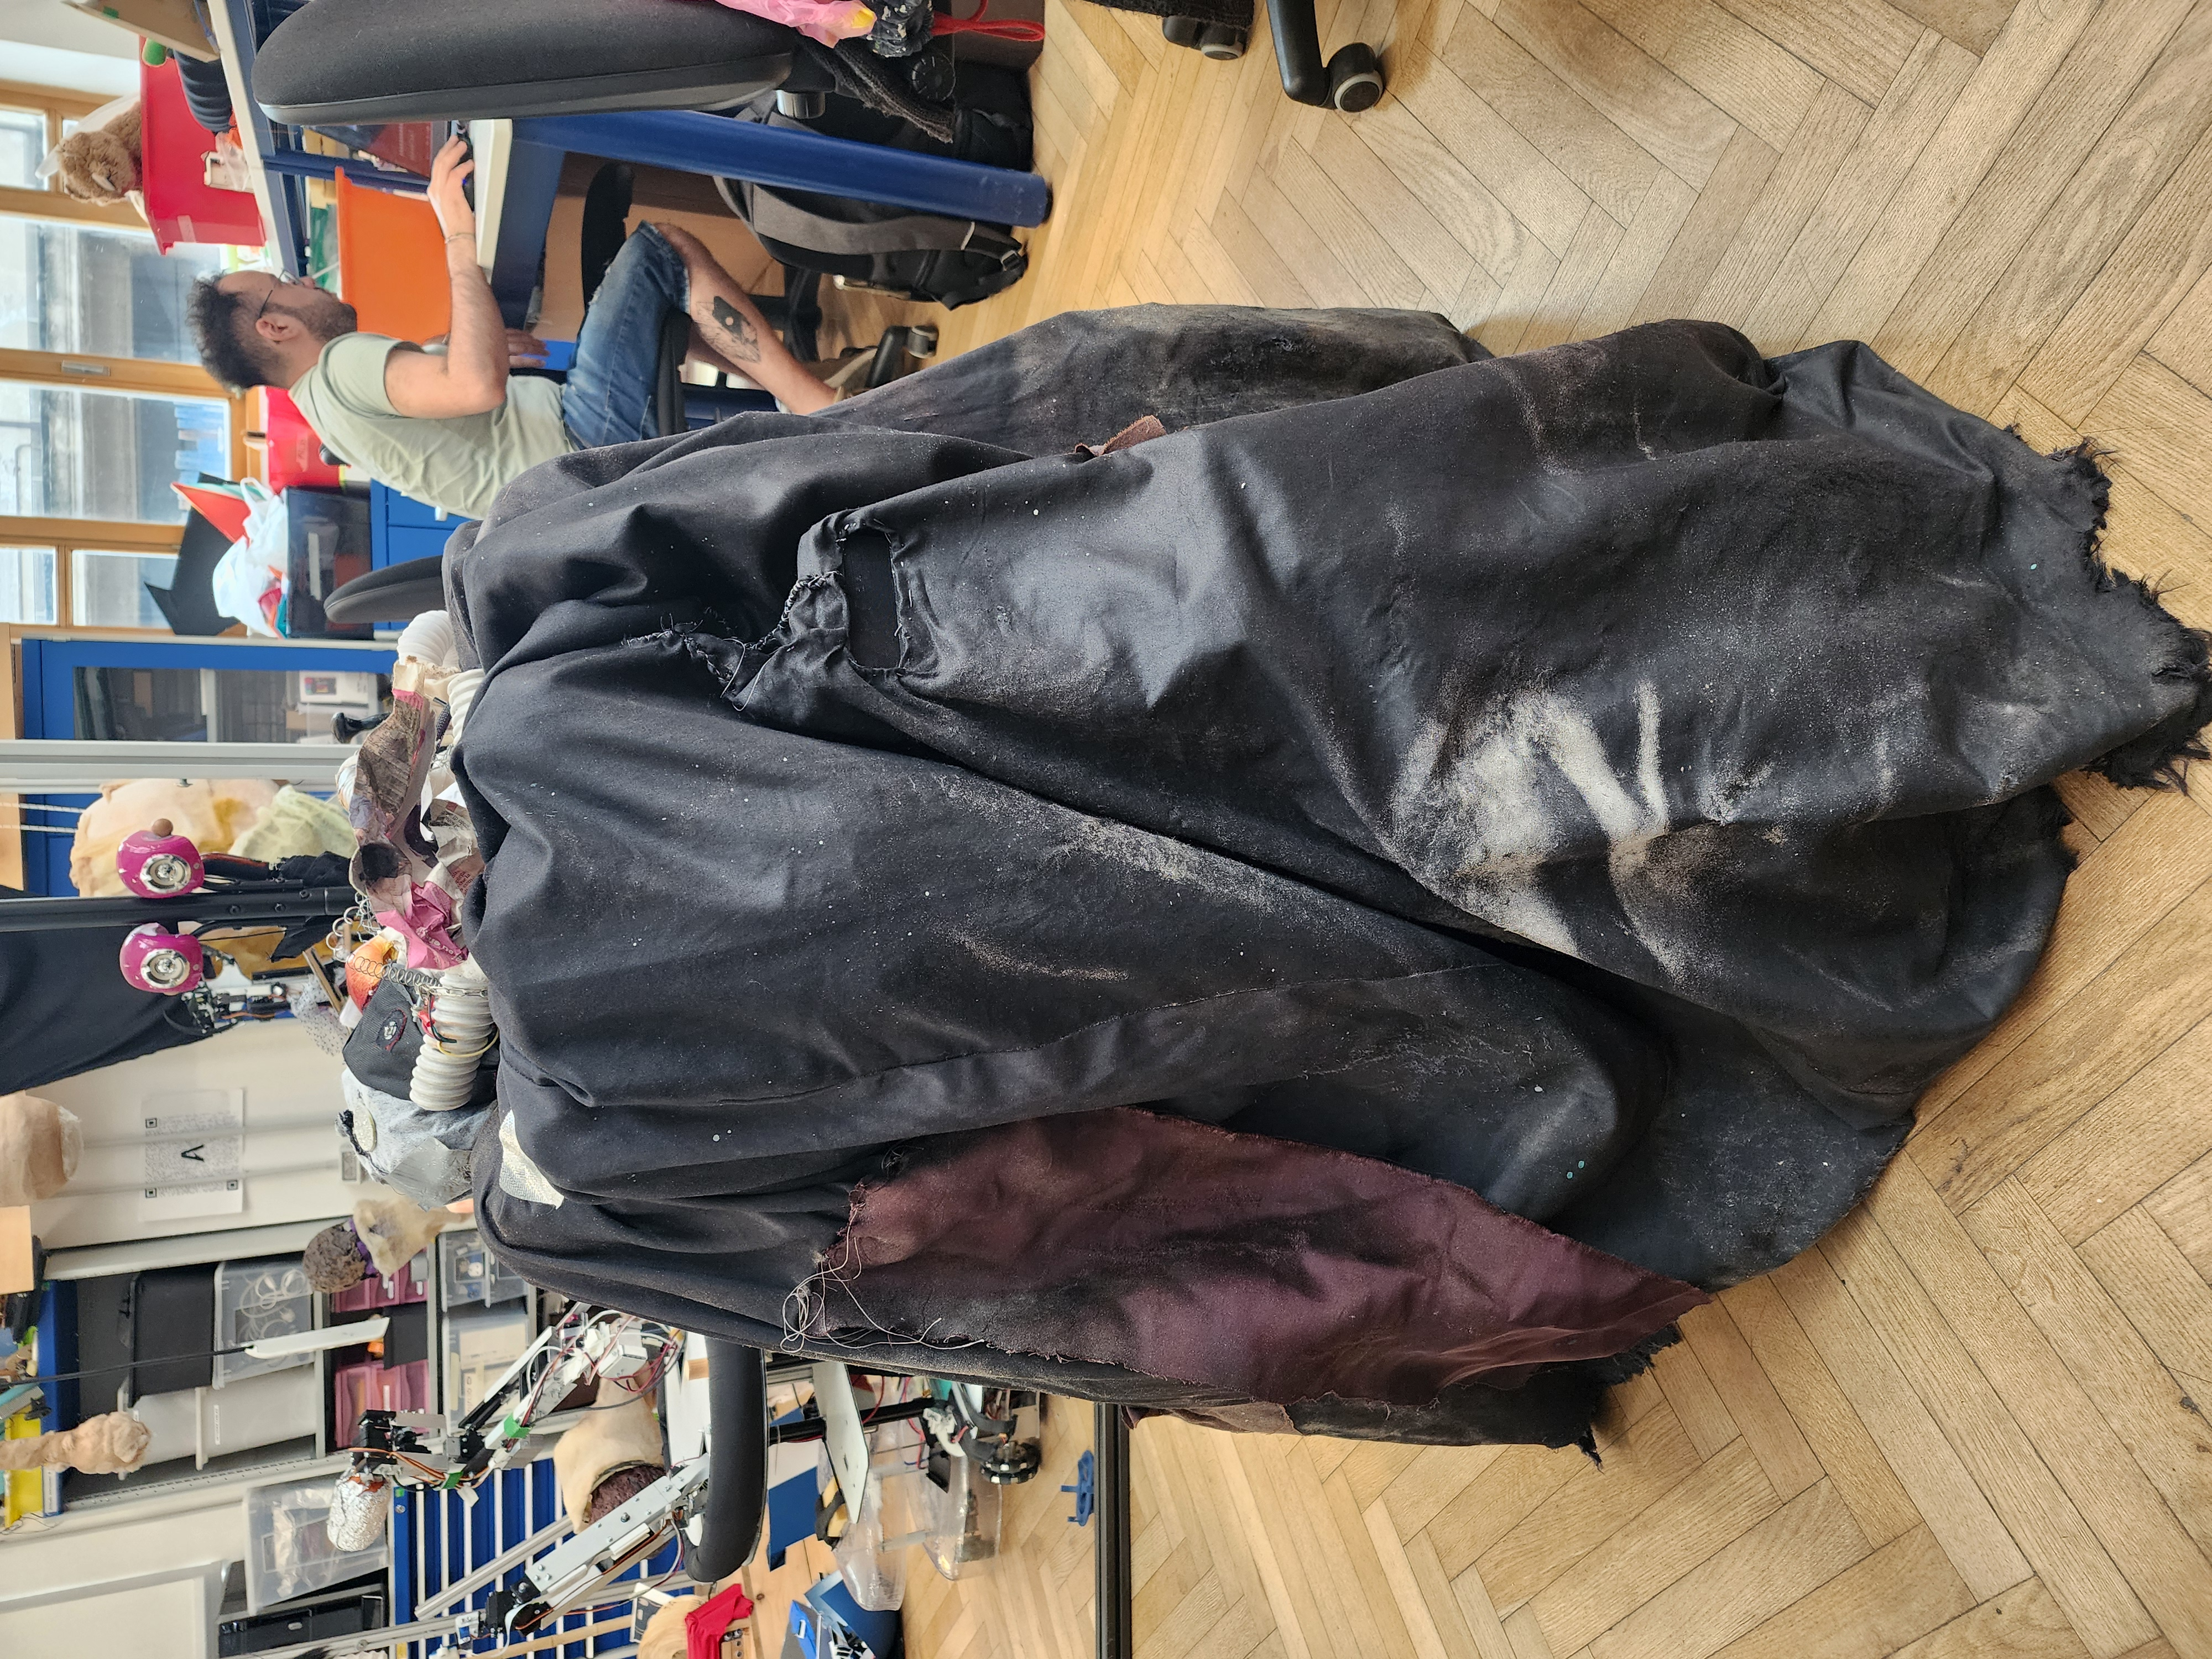
\includegraphics[width=\textwidth, angle=-90]{Images/FinalTino.jpg}
        \caption{Tino After Complete V2 Upgrade}
        \label{fig:tino_after_upgrade}
    \end{minipage}
\end{figure}

The preservation of Tino's external design language validates the holistic engineering approach that achieved dramatic internal technological advancement while maintaining the established visual identity essential for consistent human-robot interaction research. This balance between comprehensive technical modernization and aesthetic continuity ensures that the V2 platform delivers enhanced capabilities without compromising the social robotics research foundation established by the original design, enabling seamless transition to the upgraded system while maintaining research validity and experimental continuity.


\section{Hardware Implementation}
\label{sec:hardware_impl}

% REORG_TAG: moved here from Kinematic Base Upgrade from Omnidirectional to Differential Drive
\subsection{Kinematic Base Redesign}

Extended operational testing of Tino's original omnidirectional Triskar base revealed systematic mechanical failures and control complexities that threatened system reliability during social interaction research. The three-wheel omnidirectional configuration, initially selected for maximum maneuverability, proved unsuitable for Tino's 20kg operational weight and predominantly forward-motion interaction patterns.

\subsubsection{System Failure Analysis and Design Requirements}

The original Triskar platform exhibited multiple failure modes under operational demands. Omniwheel rollers experienced systematic deformation, with surfaces becoming squared due to continuous plastic deformation under Tino's weight, creating irregular rolling characteristics that manifested as vibration, reduced traction, and unpredictable movement behavior. Roller bearing failures occurred frequently in the rear omniwheel due to dragging forces during movement operations, while the three-wheel configuration created uneven weight distribution with the rear wheel experiencing excessive drag forces that accelerated component wear.

\begin{figure}[H]
    \centering
    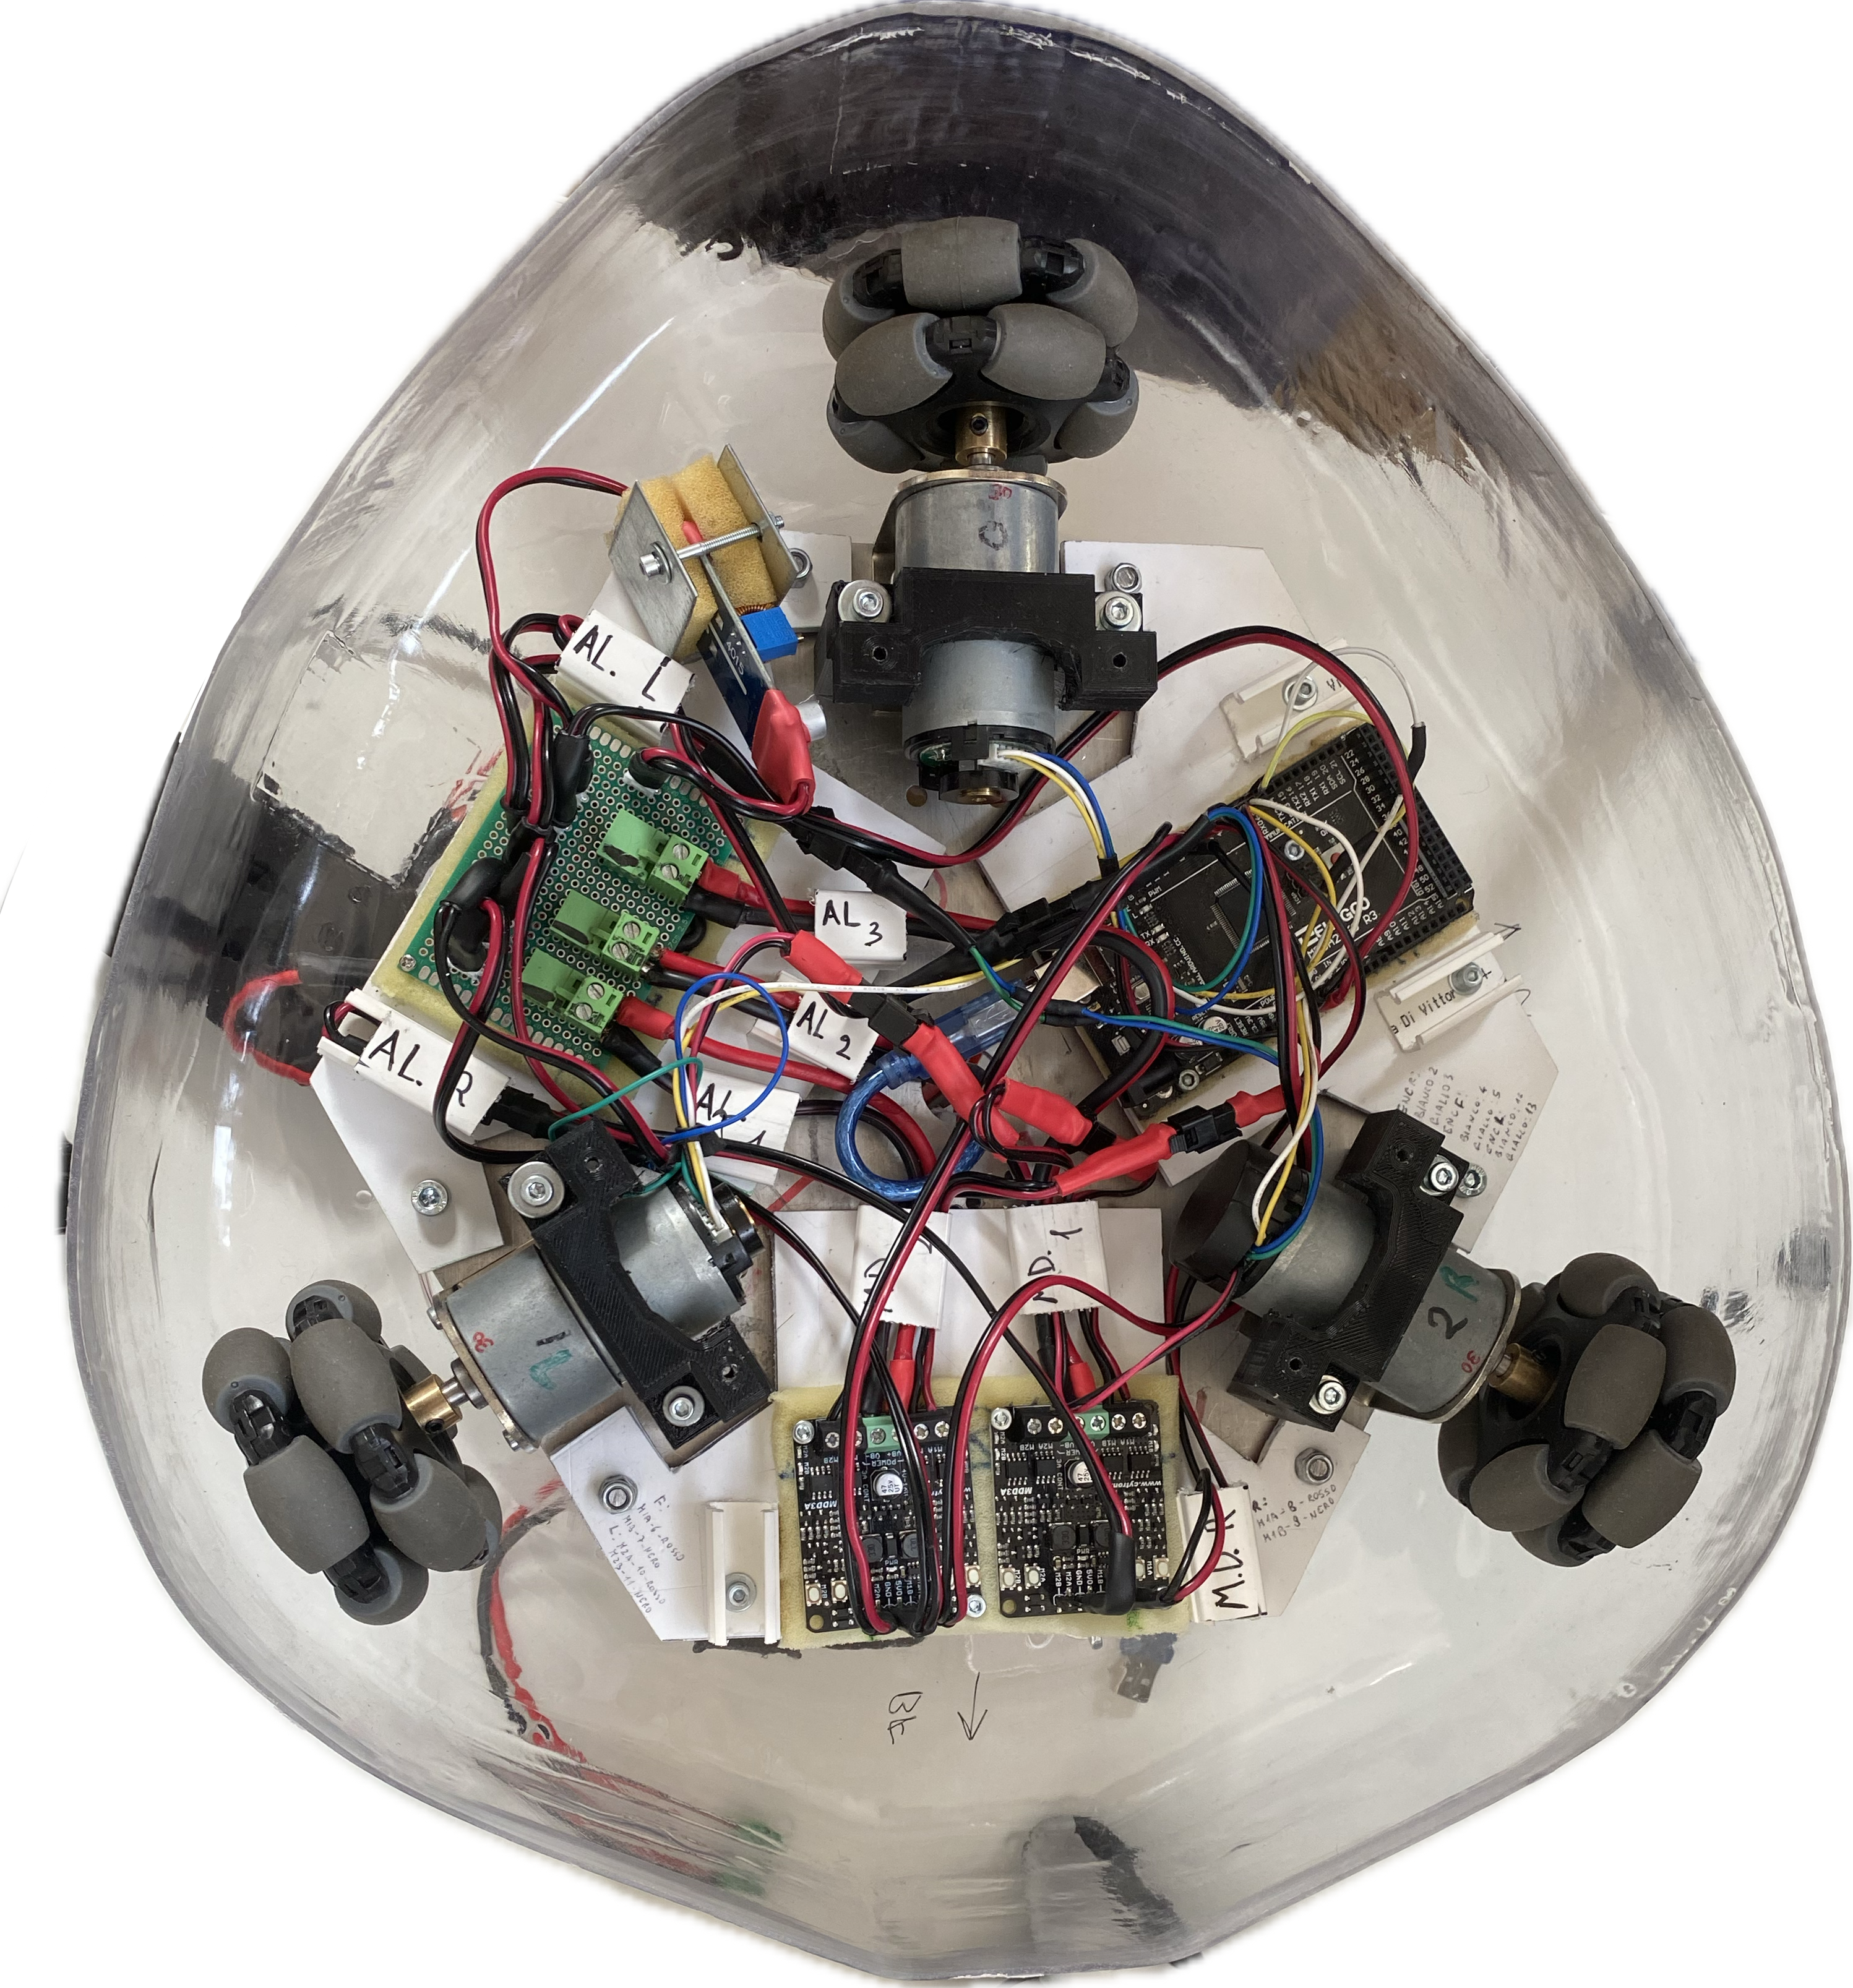
\includegraphics[width=0.5\textwidth]{Images/wire_triskar.png}
    \caption{Original Triskar Base System}
    \label{fig:original_Triskar_base}
\end{figure}

Motor performance analysis revealed inadequate torque delivery under sustained loading, with heating issues during extended use leading to performance degradation. The omnidirectional kinematics required sophisticated coordination between three drive motors while compensating for mechanical variability, creating control system complexity. Additionally, dependency on the VirHas library limited customization capabilities and created maintenance challenges for the Tino platform's specific requirements.

\subsubsection{Differential Drive Solution Design}

To address these limitations, a differential drive architecture was selected, prioritizing mechanical simplicity, enhanced reliability, and improved maintainability while providing adequate maneuverability for Tino's social interaction requirements. The design eliminates omnidirectional complexity while maintaining essential mobility through a two-wheel configuration with rear caster support that provides stable platform dynamics with reduced component count.

\begin{figure}[H]
    \centering
    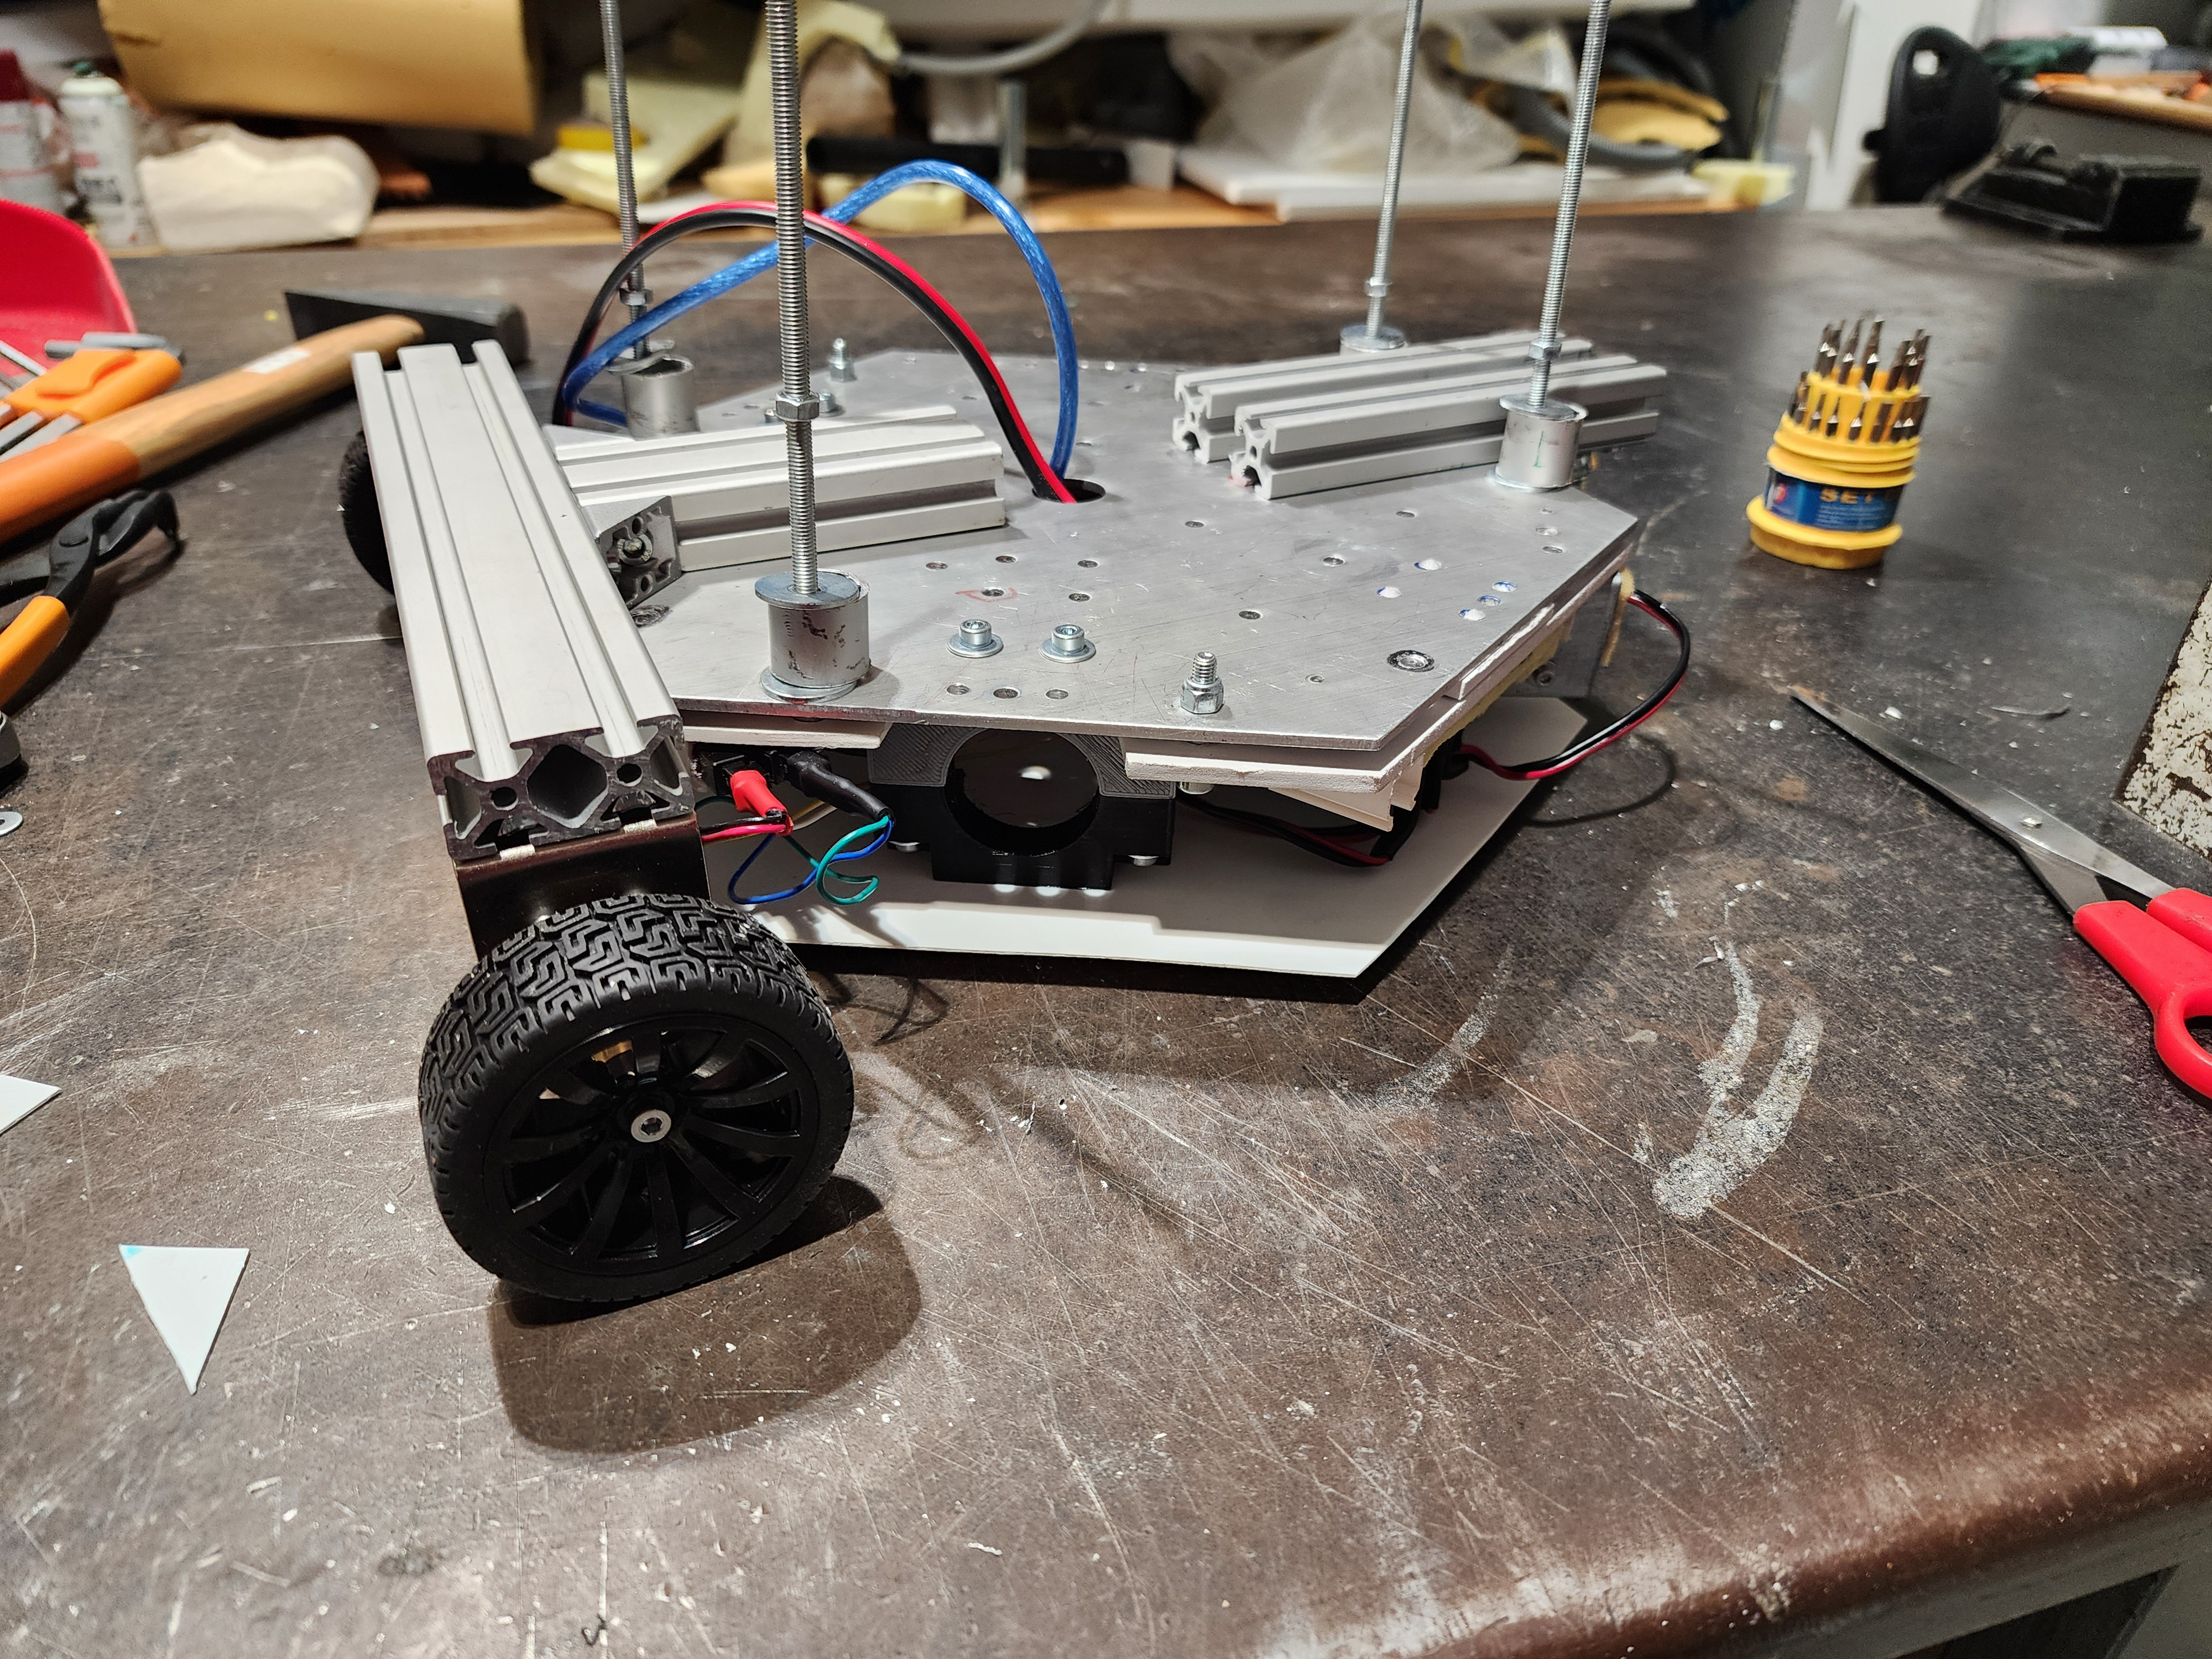
\includegraphics[width=0.7\textwidth]{Images/NewBaseDifferentialDrive.jpg}
    \caption{Complete Differential Drive Base with T-Structure Framework}
    \label{fig:differential_base_complete}
\end{figure}

Weight distribution optimization utilizes the two front drive wheels to support the majority of Tino's operational weight while the rear caster provides stability without bearing significant driving loads, eliminating the dragging forces that compromised the original system. Maneuverability analysis demonstrates that differential drive provides adequate turning capability through differential wheel speed control, with simplified kinematics enabling more precise movement control and improved repeatability. This architecture proved highly effective, providing the reliable mobility foundation necessary for supporting the enhanced computational requirements of the power system upgrade detailed in the following section.

\subsubsection{Mechanical Implementation and System Integration}

The mechanical implementation required comprehensive base reconstruction utilizing aluminum Item profiles to create a robust T-structure framework. This modular profile system provides structural rigidity while enabling mechanical adjustments without complete system redesign, with wheel spacing optimization through the adjustable T-structure enabling fine-tuning of track width to achieve proper balance and stability characteristics.

\begin{figure}[H]
    \centering
    \includegraphics[width=0.6\textwidth]{Images/NewBaseDifferentialDrive (5).jpg}
    \caption{Top View of Differential Drive Base with T-Structure}
    \label{fig:differential_base_top}
\end{figure}

Motor mounting points integrate directly with the Item profile system through custom brackets providing precise alignment and secure attachment. The motor upgrade to more powerful units addresses the thermal and torque limitations of the original system, with new motors providing enhanced heat dissipation capabilities and higher continuous torque ratings suitable for Tino's operational requirements. Motor driver upgrade to the MDD10A units provides increased current handling capability and enhanced control responsiveness compared to the original dual-driver configuration.

\begin{figure}[H]
    \centering
    \begin{minipage}{0.45\textwidth}
        \centering
        \includegraphics[width=\textwidth]{Images/NewBaseDifferentialDrive (2).jpg}
        \caption{Differential Drive Base Side View}
        \label{fig:differential_base_side}
    \end{minipage}
    \hfill
    \begin{minipage}{0.45\textwidth}
        \centering
        \includegraphics[width=\textwidth]{Images/NewBaseDifferentialDrive (3).jpg}
        \caption{Caster Wheel supporting Rear of Base}
        \label{fig:differential_base_caster}
    \end{minipage}
\end{figure}

\begin{figure}[H]
    \centering
    \begin{minipage}{0.45\textwidth}
        \centering
        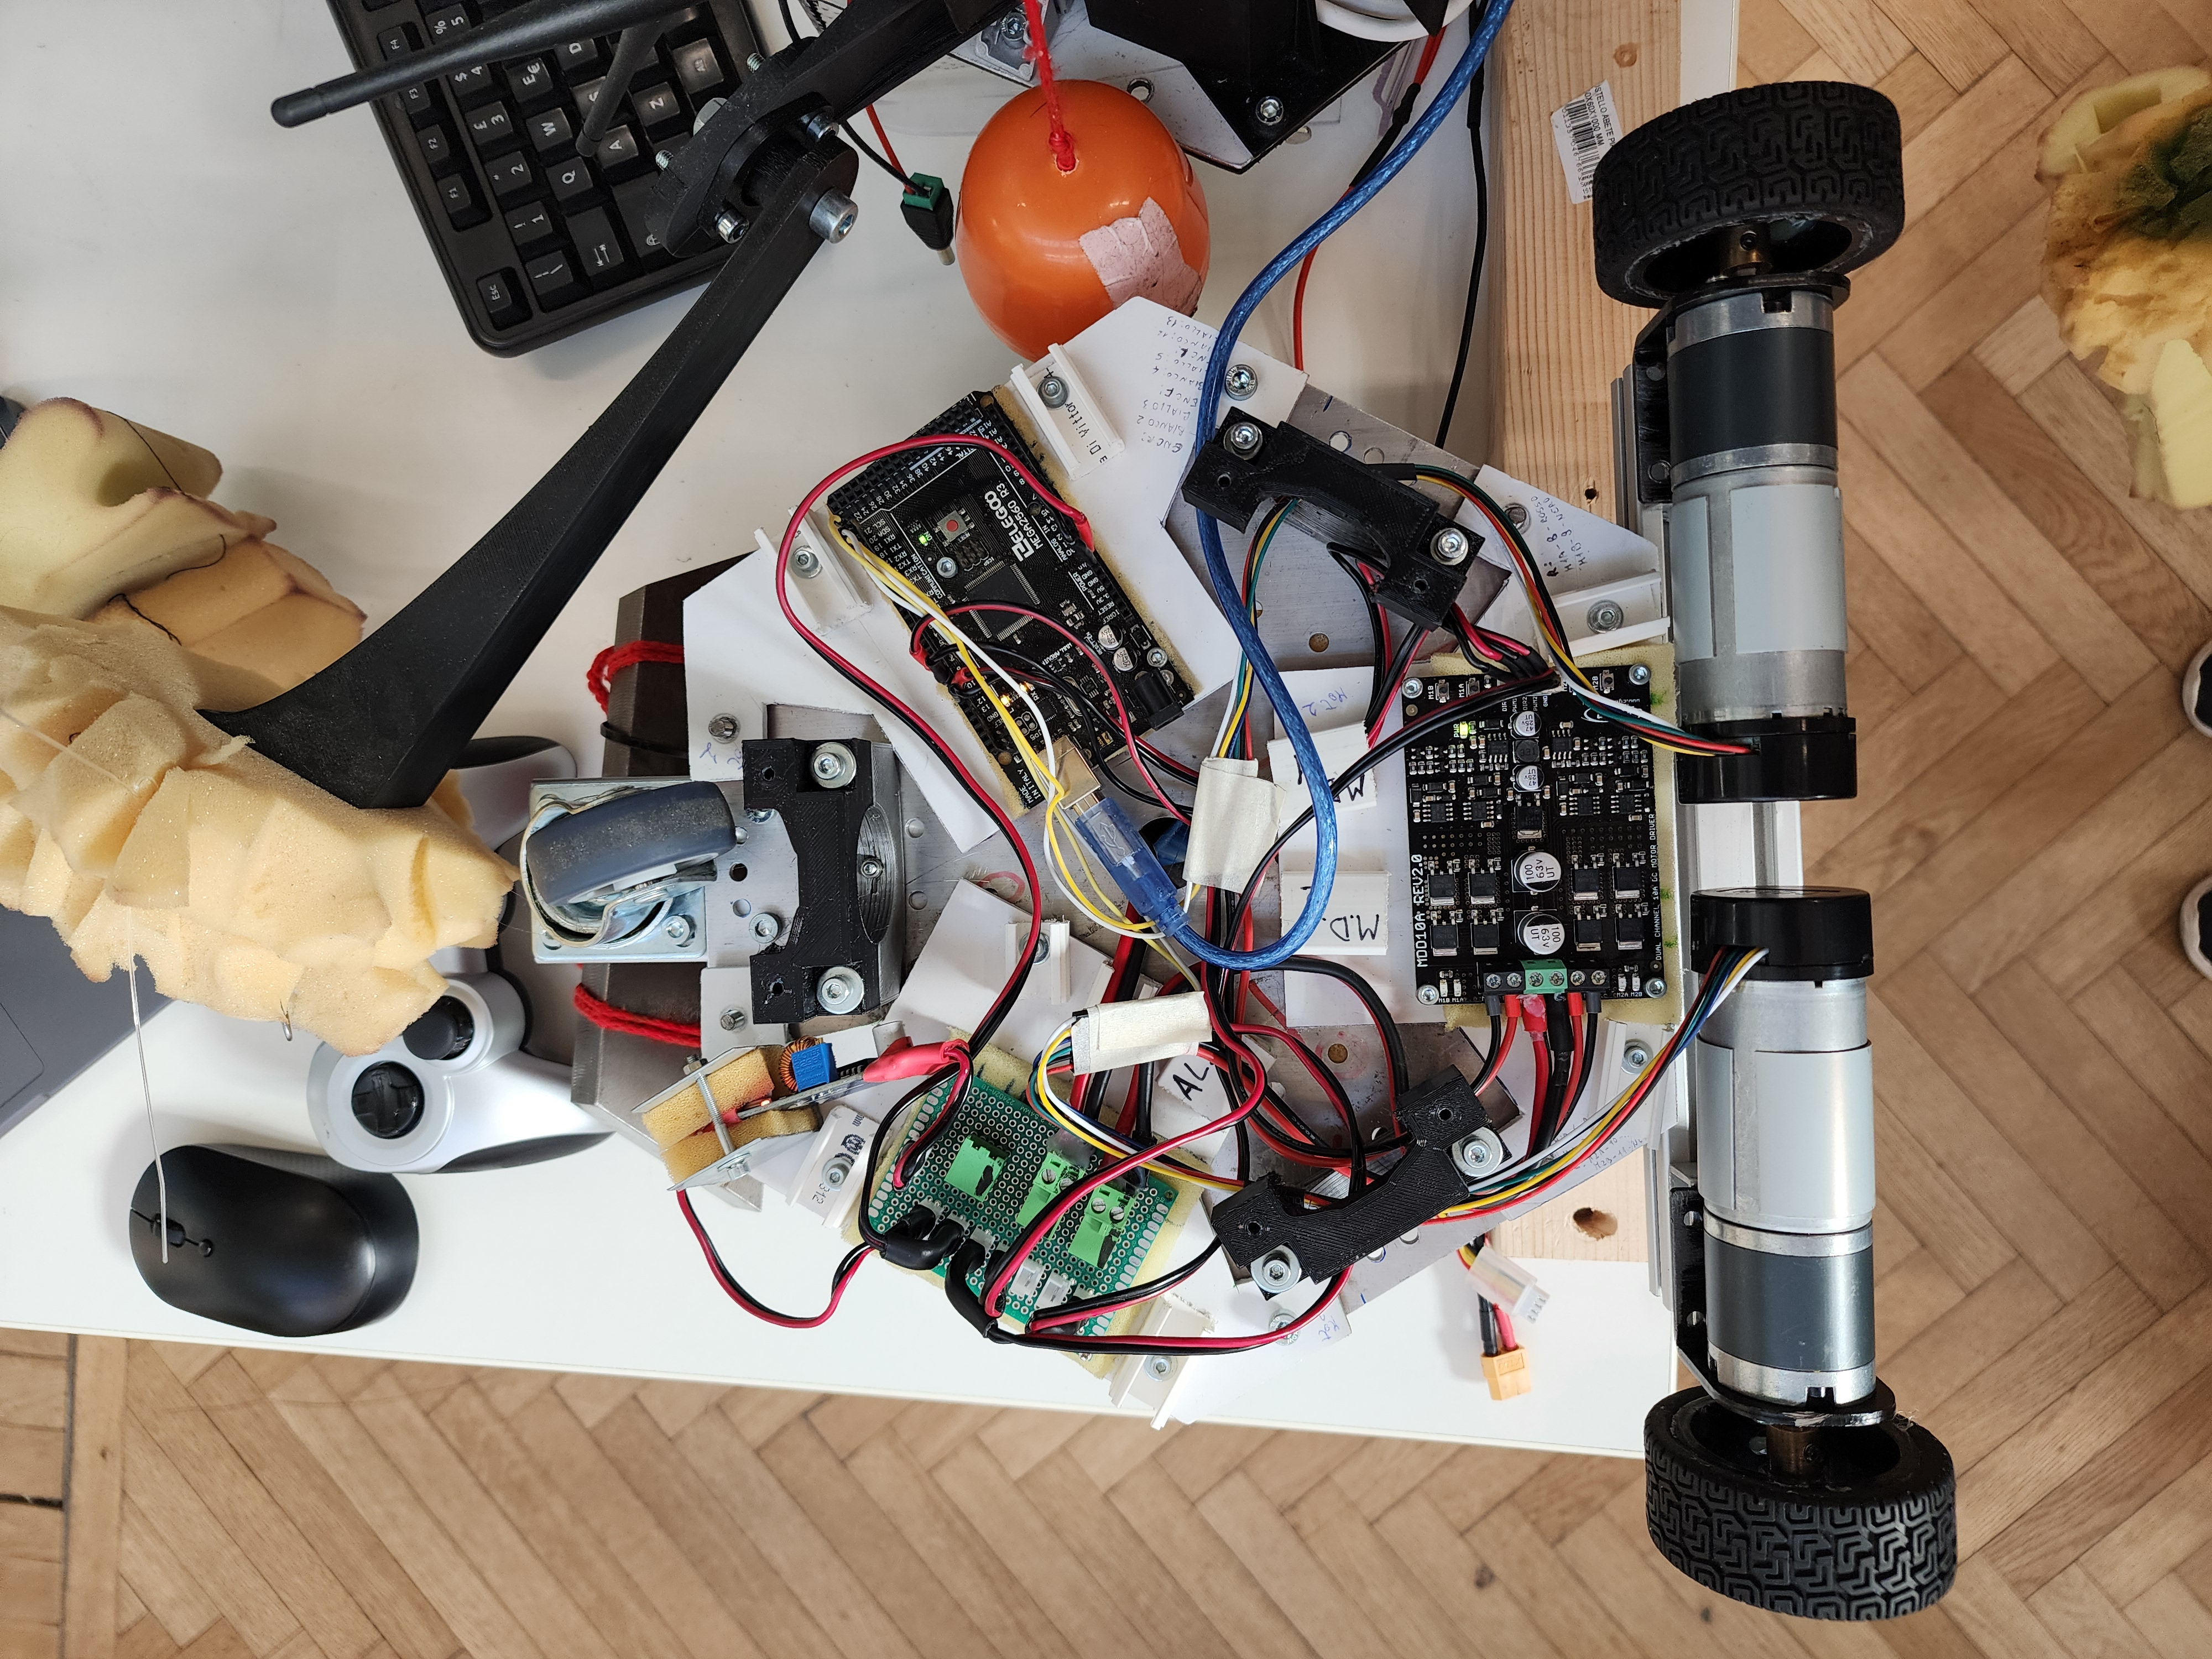
\includegraphics[width=\textwidth,angle=-90]{Images/BaseNewMotors.jpg}
        \caption{Base with New Motors (Top View)}
        \label{fig:base_new_motors}
    \end{minipage}
    \hfill
    \begin{minipage}{0.45\textwidth}
        \centering
        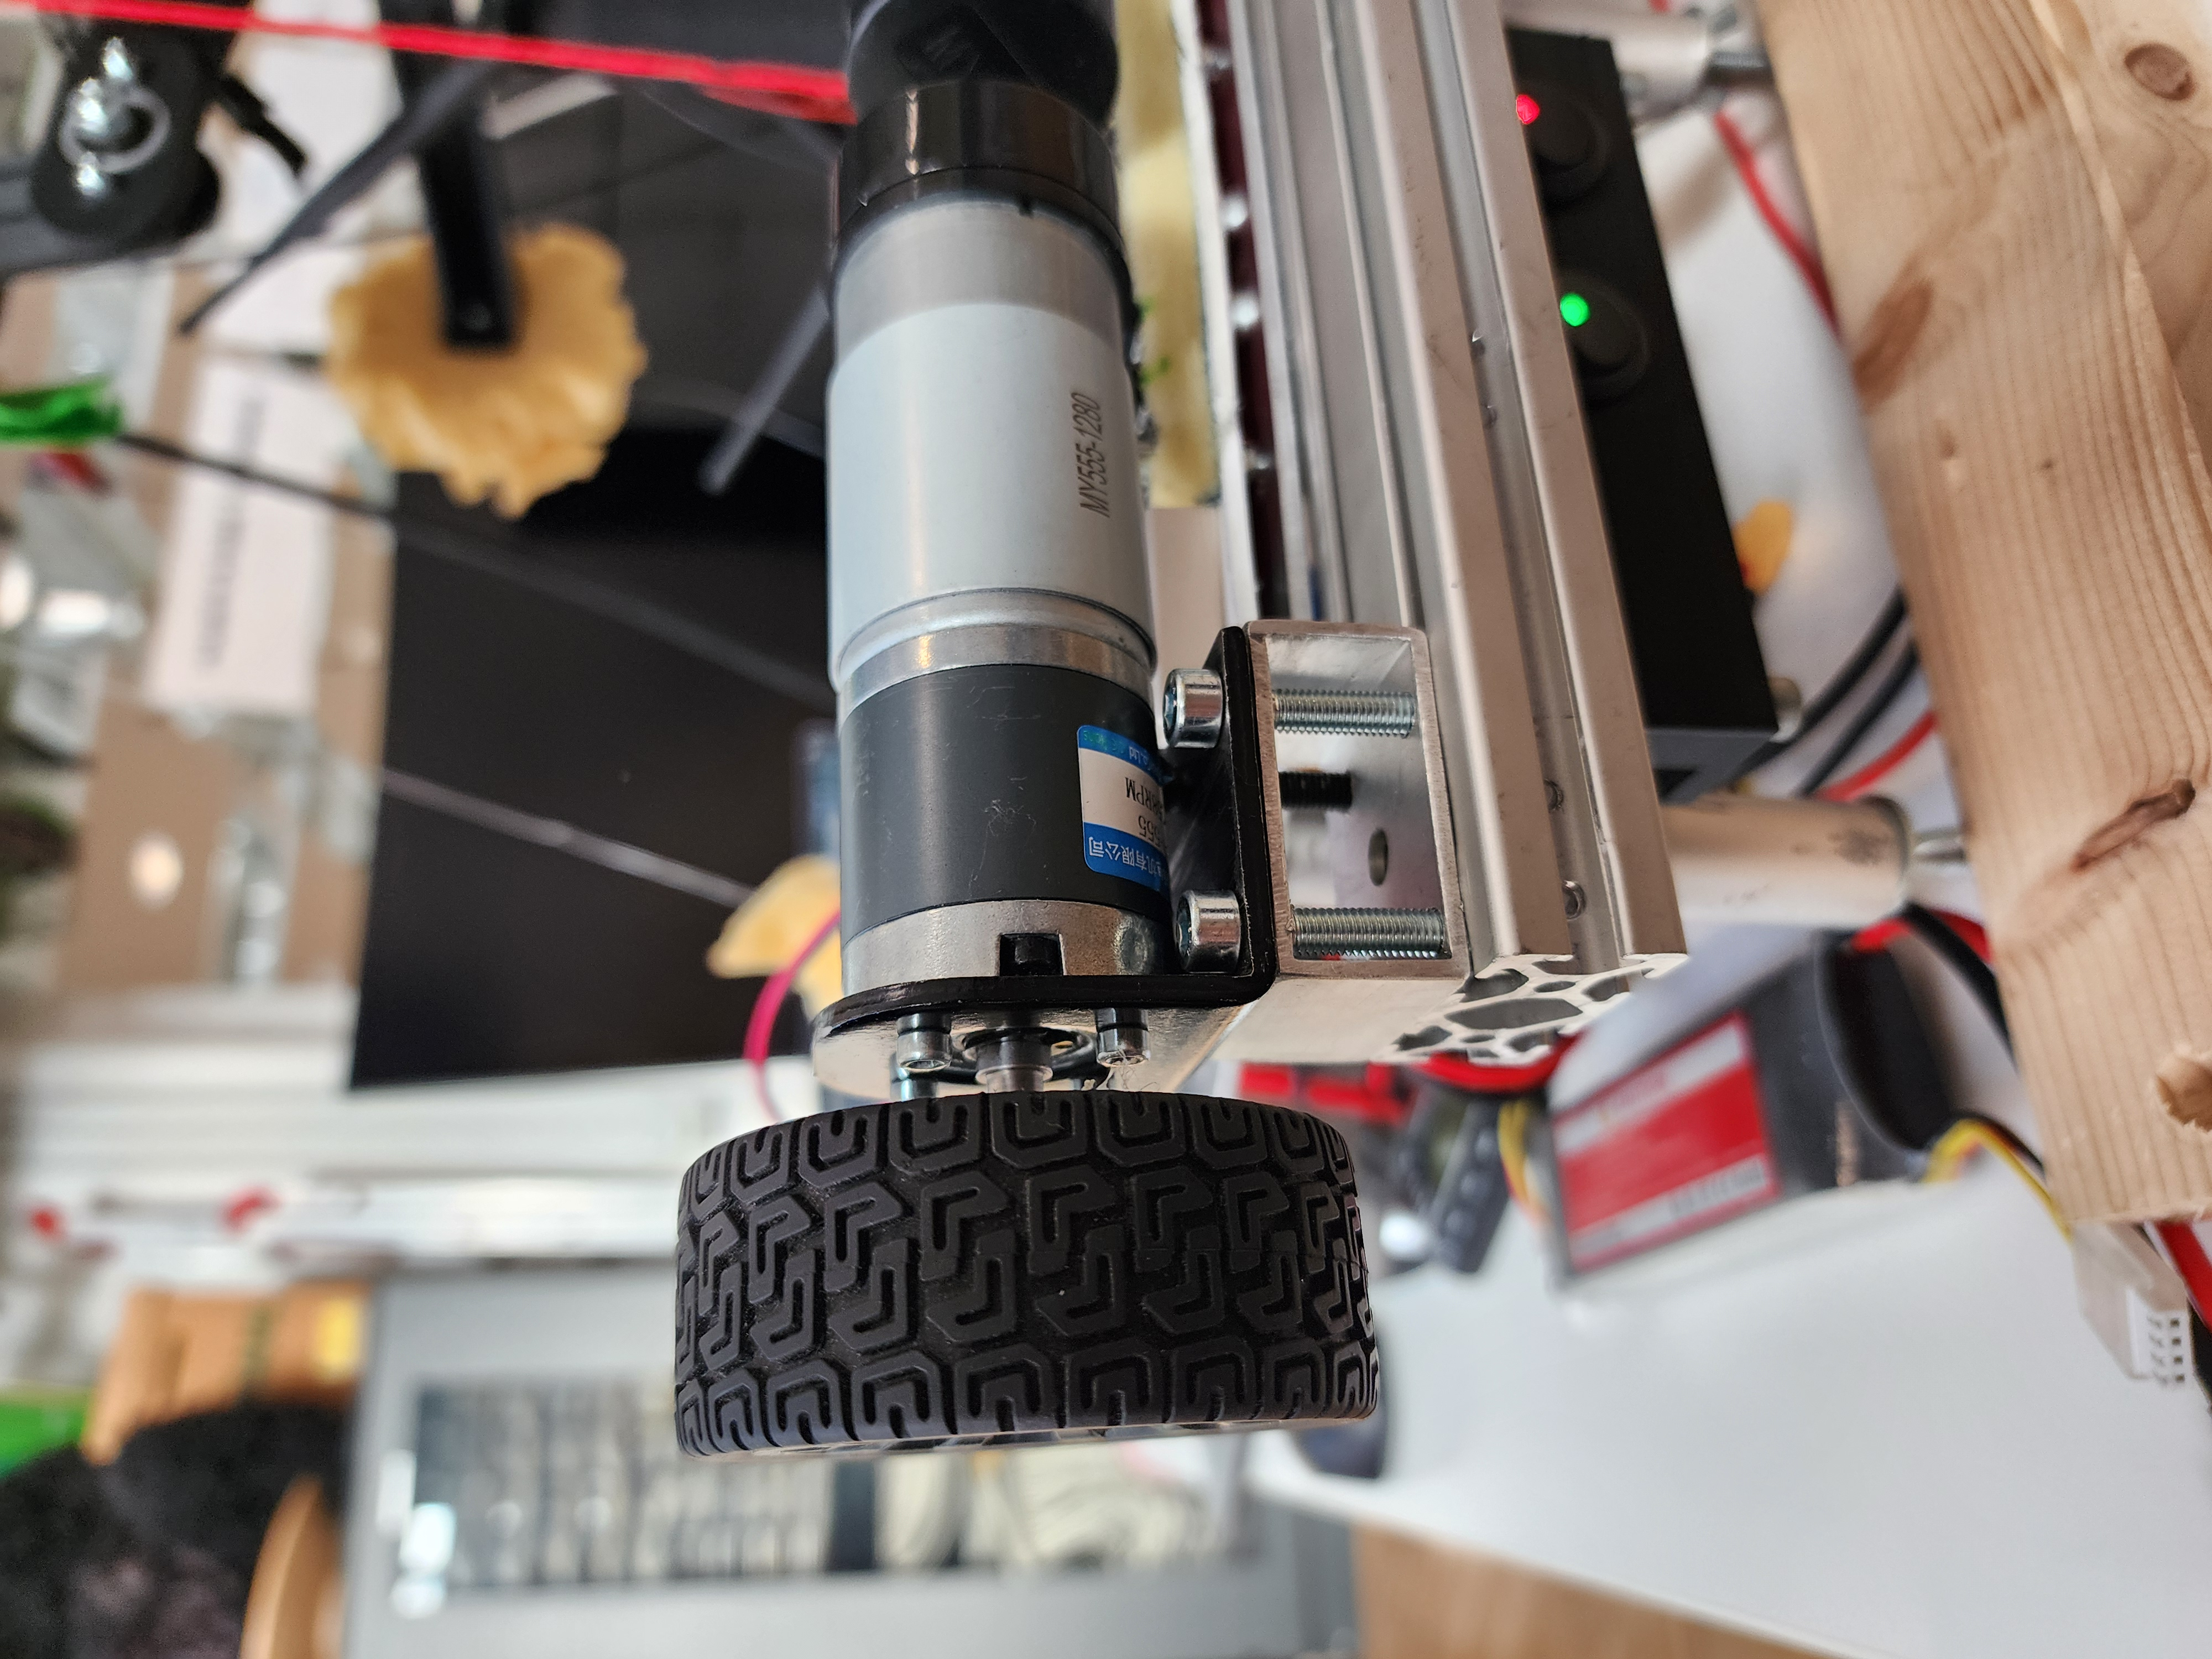
\includegraphics[width=\textwidth,angle=-90]{Images/BaseNewMotors2.jpg}
        \caption{Base with New Motors (Close up Side View)}
        \label{fig:base_new_motors_side}
    \end{minipage}
\end{figure}

\subsubsection{Wheel System and Control Integration}

The wheel selection process revealed challenges with plastic hub construction under operational loads, requiring iterative development to achieve reliable traction and durability. Initial plastic wheels with pneumatic rubber tires provided adequate traction but suffered from hub failure and tire debeading issues when rubber separated from plastic hubs due to inadequate bonding strength. The solution involved wheel hub reinforcement through hot-glue filling, which addressed structural weakness while maintaining traction characteristics, though representing a temporary fix requiring future system upgrade.

\begin{figure}[H]
    \centering
    \begin{subfigure}{0.45\textwidth}
        \centering
        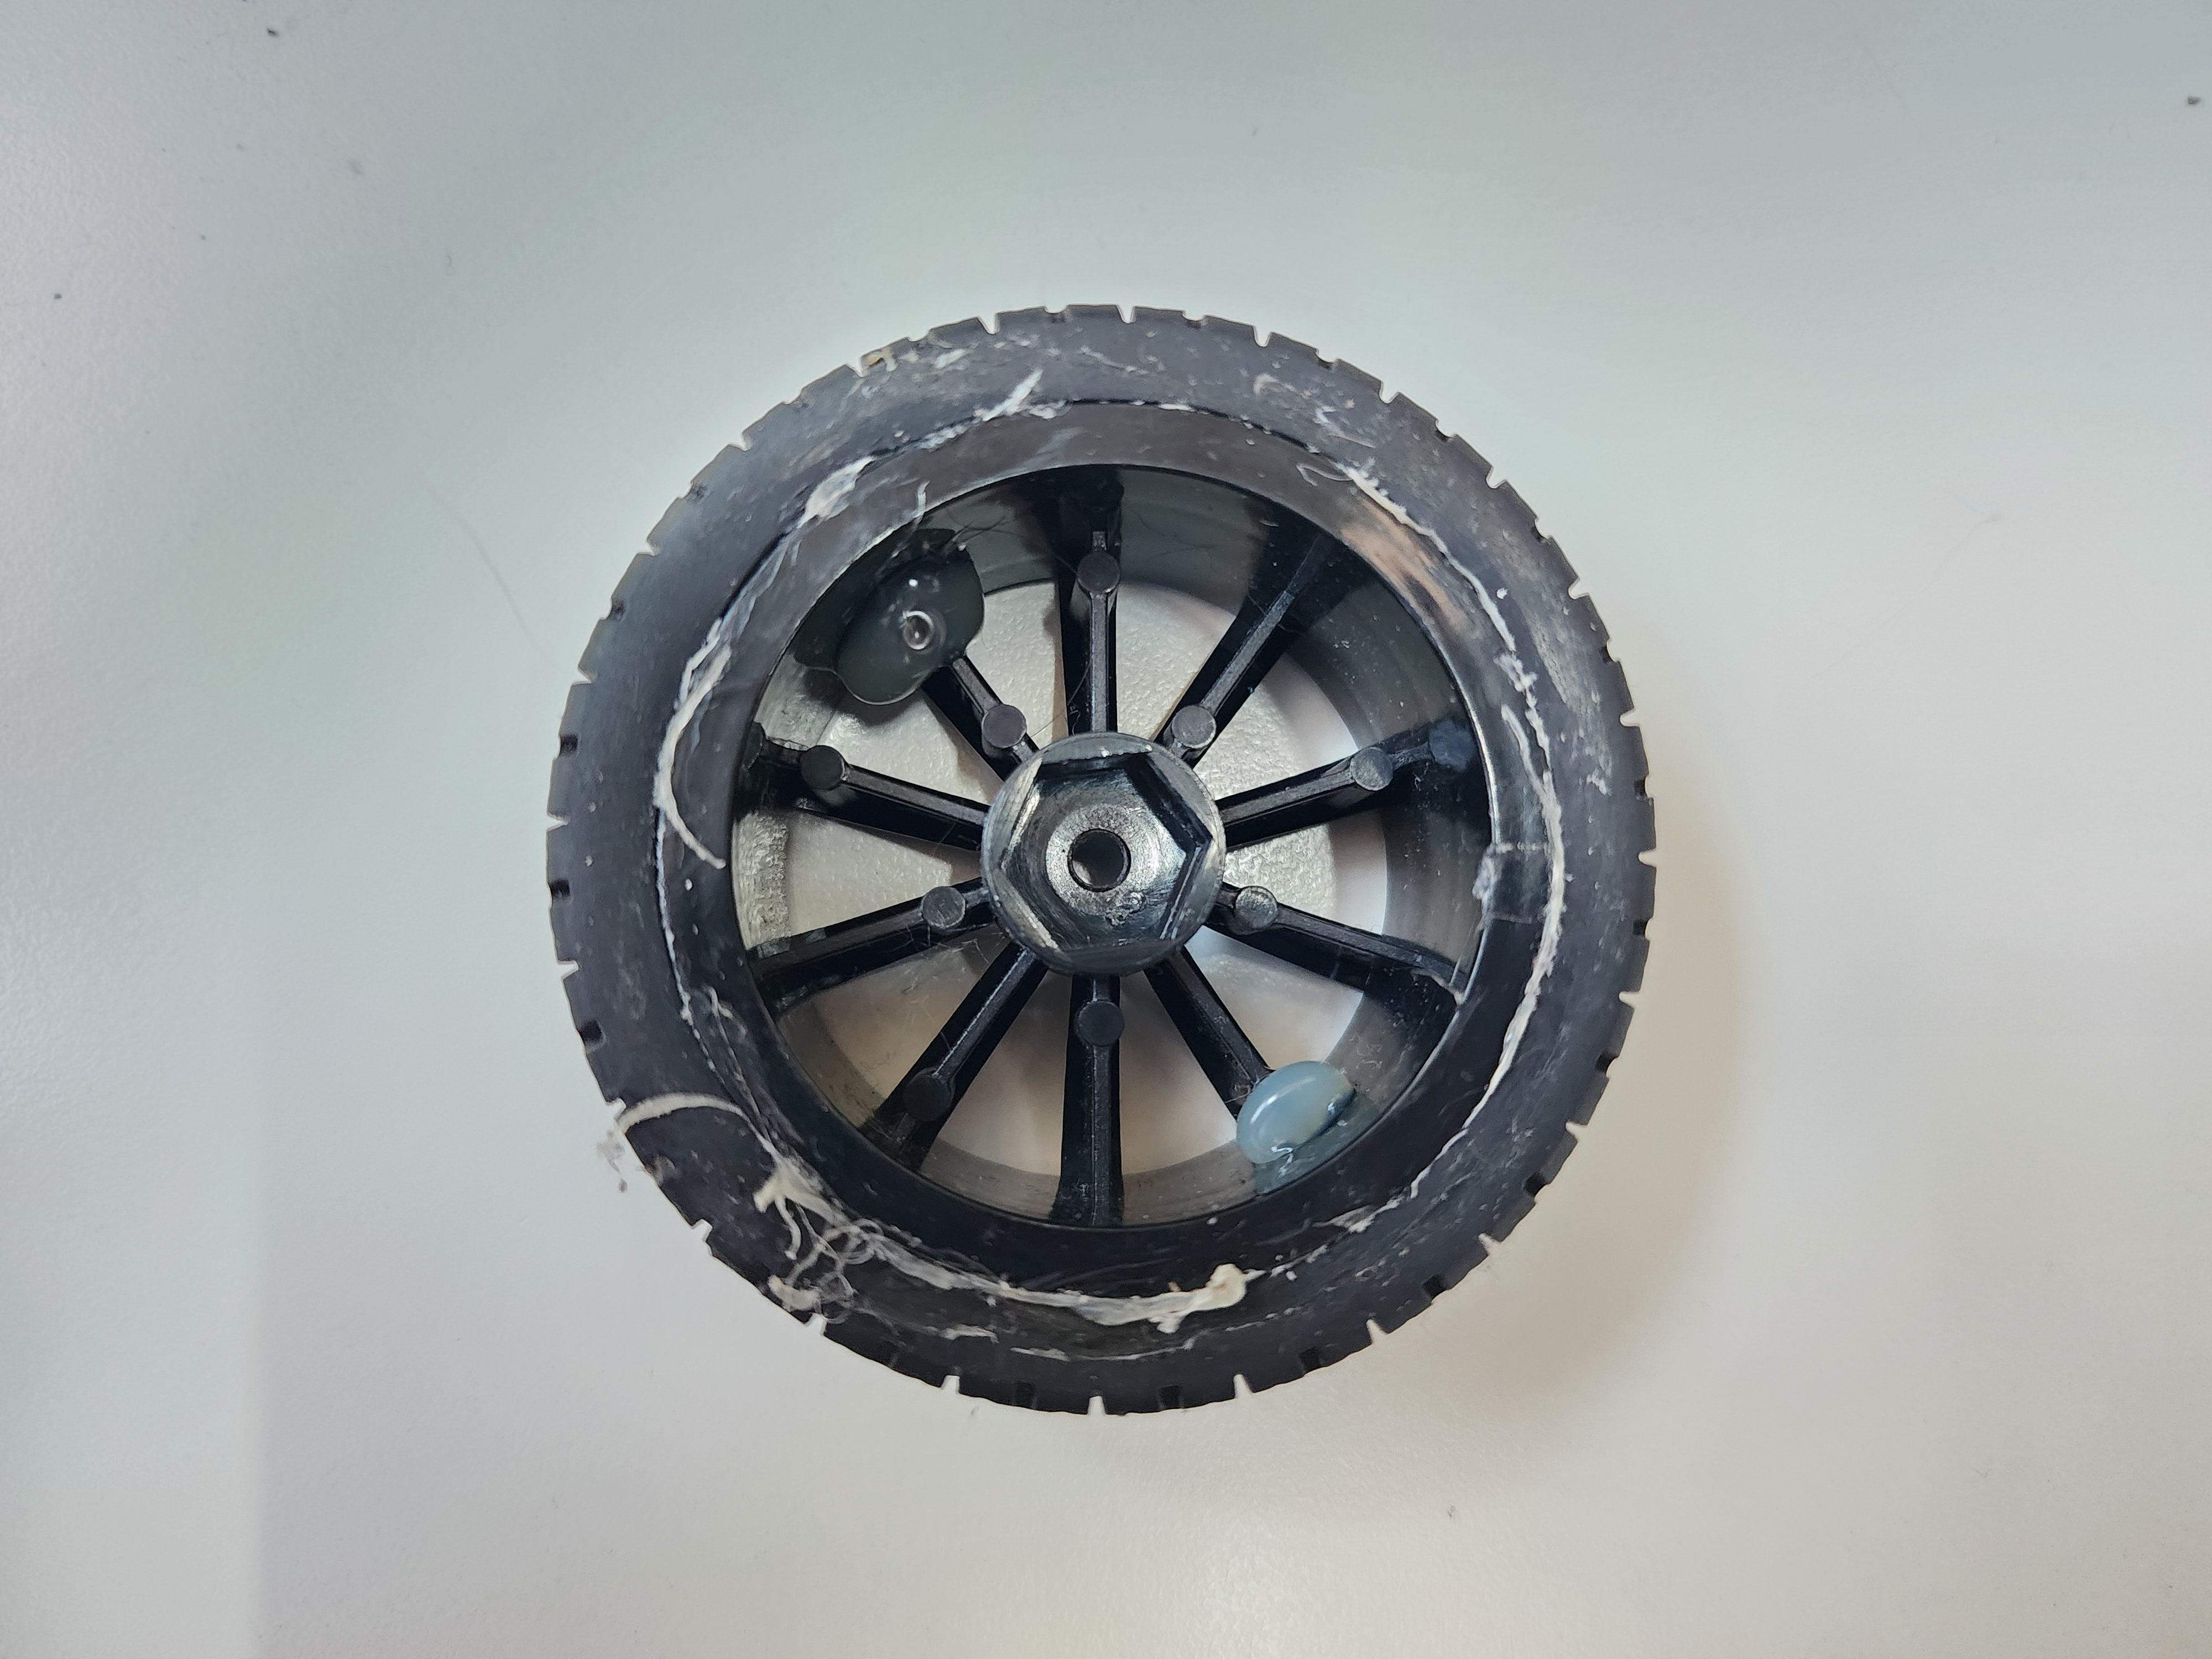
\includegraphics[width=\textwidth]{Images/WheelSilicona (3).jpg}
        \caption{Wheel Front View}
        \label{fig:wheel_hotglue}
    \end{subfigure}
    \hfill
    \begin{subfigure}{0.45\textwidth}
        \centering
        \includegraphics[width=\textwidth]{Images/WheelSilicona.jpg}
        \caption{Wheel Mounted on Motor Shaft}
        \label{fig:wheel_silicone}
    \end{subfigure}
    \caption{Wheel with Hot-Glue Filled Tires}
    \label{fig:combined}
\end{figure}

Fabric interference prevention required protective bumper implementation to prevent Tino's fabric covering from interfering with wheel operation. The bumper design provides physical separation between moving wheels and flexible fabric structure, with effectiveness testing demonstrating successful prevention of fabric entanglement in most operational scenarios.

\begin{figure}[H]
    \centering
    \includegraphics[height=6cm,angle=-90]{Images/WheelVSFabric (2).jpg}
    \caption{Wheel vs Fabric Interference}
    \label{fig:wheel_vs_fabric}
\end{figure}

\begin{figure}[H]
    \centering
    \begin{minipage}{0.45\textwidth}
        \centering
        \includegraphics[width=\textwidth]{Images/TinoBumper (4).jpg}
        \caption{Tino Bumper Front View}
        \label{fig:tino_bumper_front}
    \end{minipage}
    \hfill
    \begin{minipage}{0.45\textwidth}
        \centering
        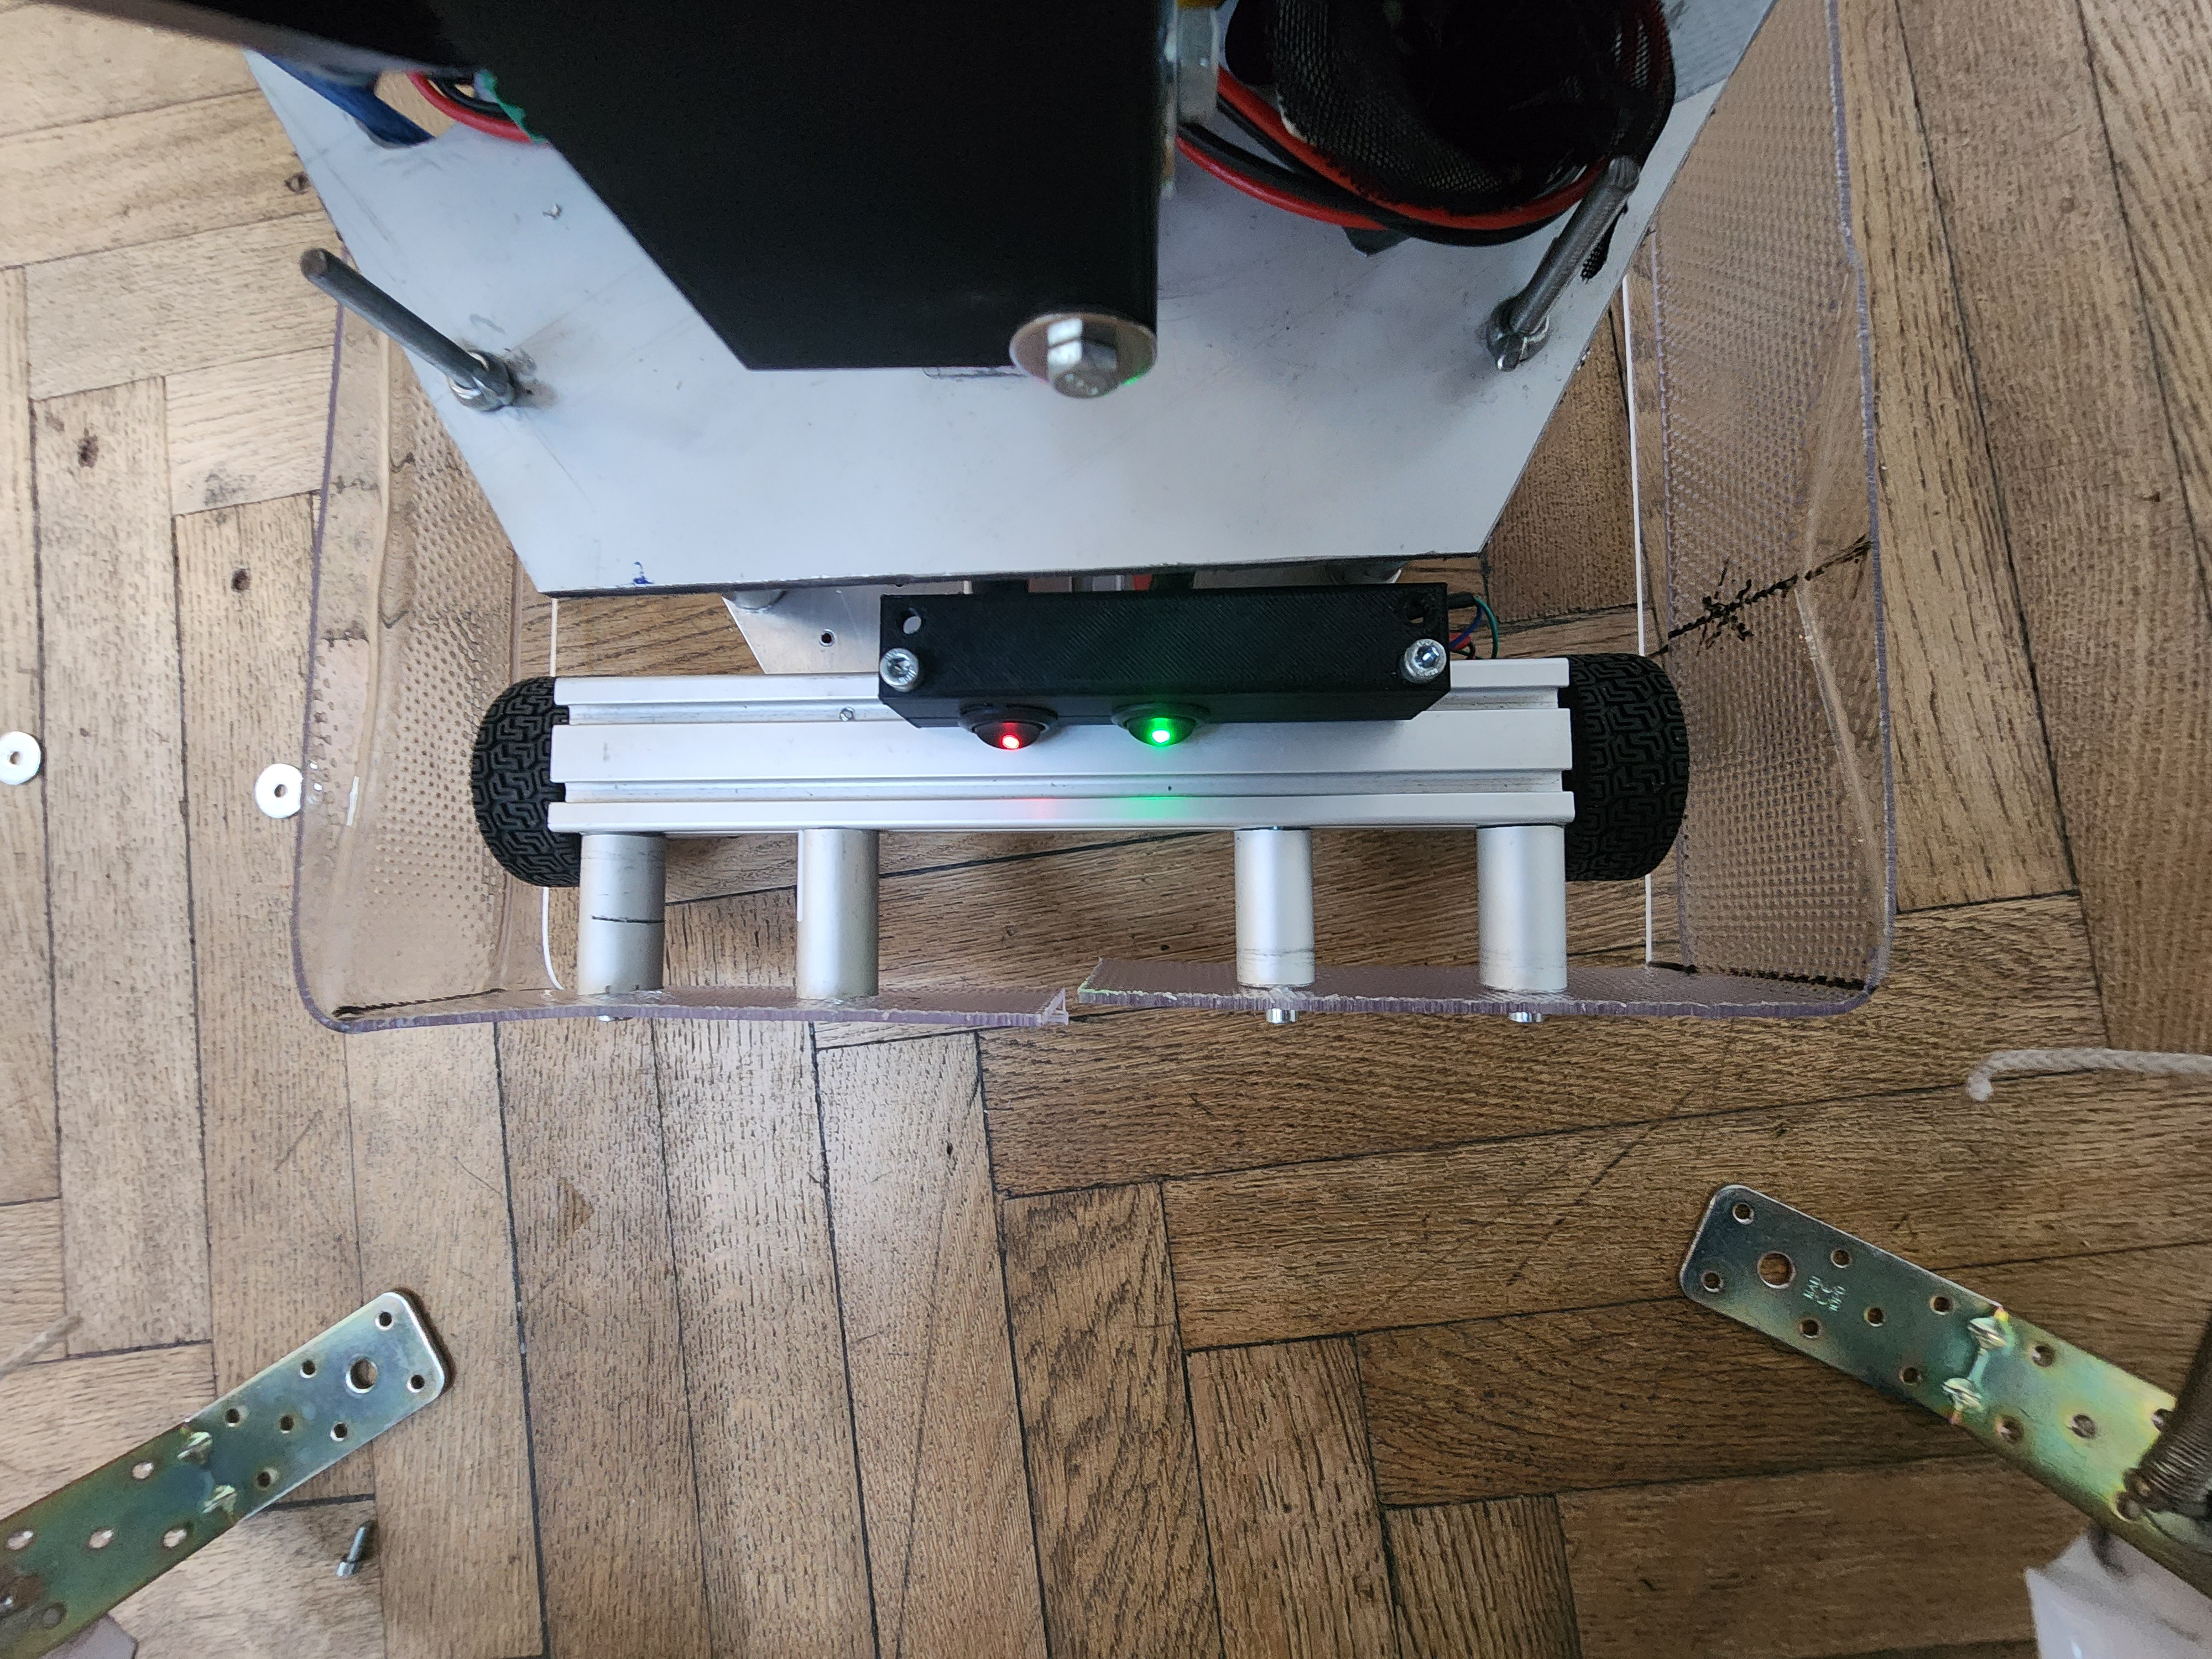
\includegraphics[width=\textwidth]{Images/TinoBumper (5).jpg}
        \caption{Tino Bumper Top View}
        \label{fig:tino_bumper_top}
    \end{minipage}
\end{figure}

The control system adaptation required comprehensive modification to support differential drive kinematics while maintaining compatibility with existing command interfaces. A custom PID controller was developed specifically for differential drive characteristics, replacing the VirHas library with optimized algorithms utilizing Kp=7.3, Ki=5.6, and Kd=0.2 parameters tuned for MDD10A motor drivers. Motor speed calculation employs encoder feedback with 1920 pulses per revolution (PPR) encoders, while atomic movement control integrates four distinct movement states that support synchronized leg-base coordination for VR integration.

\begin{figure}[H]
    \centering    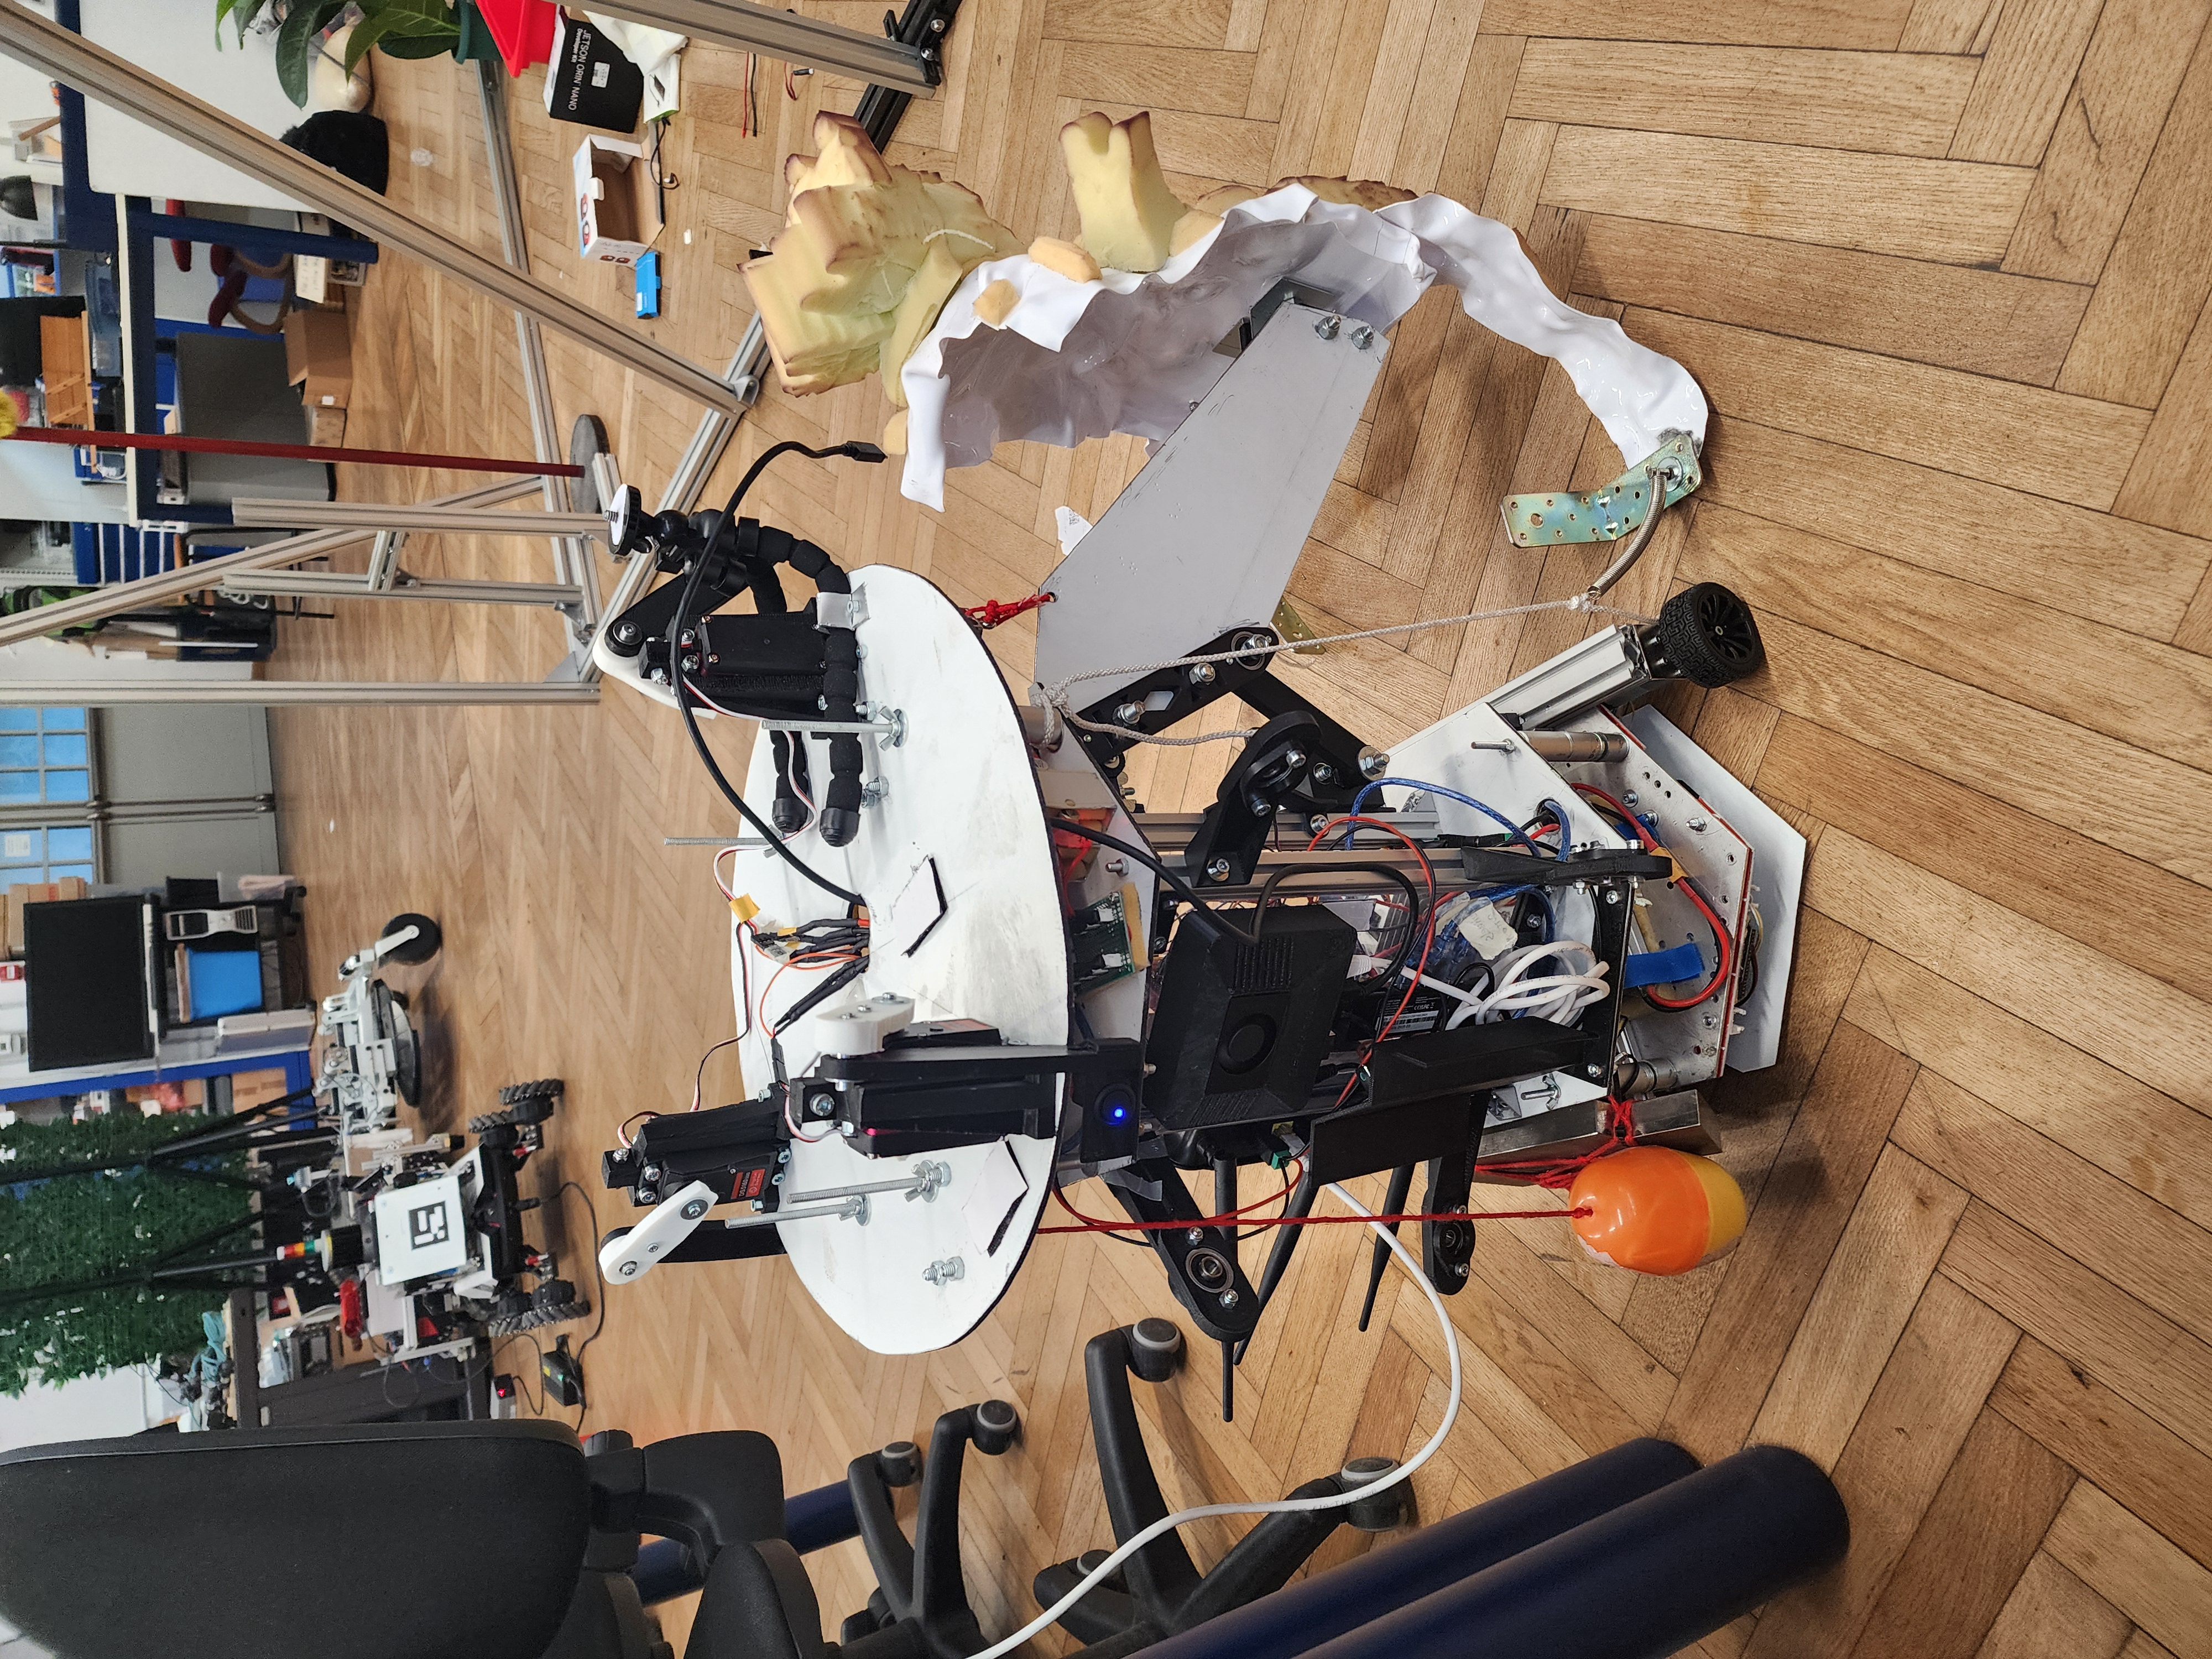
\includegraphics[width=0.8\textwidth, angle=-90]{Images/TinoOnNewBase.jpg}
    \caption{Tino's new Base}
    \label{fig:tino_on_new_base}
\end{figure}

Motor speed calculation employs encoder feedback with 1920 pulses per revolution (PPR) encoders through the \texttt{getMotorSpeed()} function, enabling closed-loop speed control for precise movement execution. The \texttt{updatePid()} function implements the complete PID algorithm with integral term reset, derivative damping, and output limiting to ±255 PWM range, ensuring stable motor control without oscillation.

The \texttt{updateBaseMovementByTime()} function manages four distinct movement states that implement atomic operation completion where each movement phase must finish before accepting new commands. This prevents interrupted motions that could compromise synchronized robot behavior during VR integration. With the kinematic base providing reliable mobility, the system required enhanced power delivery capabilities to support the computational demands of the upgraded processing platform.

\subsection{Power Supply System}

The transition from Raspberry Pi to NVIDIA Orin Nano necessitated complete power system redesign to support significantly higher computational loads and multiple high-performance components. The legacy Raspberry Pi power distribution system proved inadequate for the Orin Nano's 19V DC requirement, Oak-D Pro camera power demands, and enhanced router system, requiring comprehensive architecture overhaul with consolidated battery management and efficient DC-DC conversion.

\subsubsection{System Requirements and Power Analysis}

The Orin Nano requires 19V DC input with power consumption reaching up to 2A during maximum computational load scenarios including simultaneous SLAM processing, human detection, audio processing, and ROS2 node operation. Typical operational consumption ranges between 1.3A to 1.4A during standard social interaction scenarios, with peak consumption of 38W during maximum load conditions and sustained operation typically requiring 25--27W. The power profile exhibits significant variation based on computational load, requiring robust power delivery capable of handling transient peaks without voltage drop.

Auxiliary system requirements include the Oak-D Pro camera system requiring 5V DC input with power consumption up to 5W during high-resolution stereo processing, and the onboard router system requiring 5V DC input with approximately 3W consumption during operational periods. Total system power budget analysis indicates maximum power consumption of approximately 46W under peak operational conditions, with typical sustained operation requiring 33--35W.

\subsubsection{Power Conversion and Distribution Implementation}

The power conversion system utilizes high-efficiency DC-DC converters to transform battery voltage to the multiple voltage levels required by system components. The Oumefar DC-DC step-up converter provides stable 19V output from 12V battery input with efficiency ratings exceeding 85\% across the operational load range, with converter selection prioritizing stability, efficiency, and thermal performance under sustained loading conditions. Power delivery stability testing demonstrated consistent voltage regulation within ±2\% across full load range with excellent transient response during computational load variations.

The 12V to 5V conversion system provides power for auxiliary components including the Oak-D Pro camera and onboard router, with power distribution architecture enabling independent power control for auxiliary components. 

\subsubsection{Battery System Consolidation and Performance}

The battery system redesign consolidates multiple power sources while providing enhanced capacity and reliability for extended operational periods. The primary battery system utilizes 5200mAh 80C 11.1V 57.72Wh LiPo batteries that provide the power density and discharge capabilities required for robotic applications, with battery specification analysis demonstrating adequate capacity for 2--3 hours of typical operation with conservative discharge management.

Maximum load operational time calculations indicate approximately 1.37 hours of operation under peak power conditions, though realistic operational scenarios typically achieve 2+ hours due to variable computational loading. The high discharge rate capability (80C) ensures stable power delivery during computational peaks without voltage sag, while the system consolidation reduces complexity from four separate battery systems to three integrated power sources.

The cable harness redesign eliminates obsolete USB-A and USB-C connections utilized for Raspberry Pi power delivery, replacing them with proper 12V distribution and 19V DC jack connectivity optimized for Orin Nano requirements. The 12V input distribution system provides primary power for both the step-up converter and the secondary 5V converter, with the 19V DC jack implementation providing secure power connection to the Orin Nano with proper mechanical support and electrical contact reliability.
% REORG_TAG: moved here from Stewart Platform Head Mechanism Improvements
\subsection{Stewart Platform Head Mechanism}

The Stewart platform head mechanism required iterative design improvements to address systematic reliability issues encountered during extended operational periods. The original implementation exhibited servo axis misalignment that created excessive stress concentrations on servo motor internals during head movement operations, with force analysis revealing that head loads were transmitted directly through servo shafts rather than through the structural framework. Additionally, the connecting arms showed excessive structural flexibility that reduced head positioning precision and contributed to mechanical instability, with repeated arm failures occurring due to inadequate load distribution and material selection in the 3D printed PLA components.

\begin{figure}[H]
    \centering
    \includegraphics[height=6cm]{Images/signle_head_motor.jpg}
    \caption{Head Arm V0 Design}
    \label{fig:head_arm_v0}
\end{figure}

\subsubsection{Design Evolution and Failure Resolution}

The first design iteration focused on servo axis alignment to redirect forces through proper load paths while maintaining the existing bearing-based connection system. The servo axis alignment improvement redirected head loads through the structural framework rather than servo mechanisms, with enhanced PLA arm geometry providing improved load distribution through optimized cross-sectional design and stress concentration reduction.

\begin{figure}[H]
    \centering
    \includegraphics[height=6cm, angle=-90]{Images/HeadArmV2.jpg}
    \caption{Head Arm V1 Design}
    \label{fig:head_arm_v1}
\end{figure}

Performance evaluation demonstrated reduced servo stress indicators and improved movement precision, though structural flexibility issues remained due to the retained bearing connection system. Despite these improvements, the Stewart platform continued to experience significant structural flexibility problems that led to repeated arm failures during extended operational periods.

\begin{figure}[H]
    \centering
    \includegraphics[height=6cm, angle=-90]{Images/HeadArmFailure (2).jpg}
    \caption{Head Arm Failure after Extended Use}
    \label{fig:head_arm_failure}
\end{figure}

The bearing connection system on the servo side of each arm introduced excessive compliance that compromised head positioning precision and contributed to continued mechanical instability. Failure analysis revealed that the 3D printed bearing housings could not adequately transfer forces between the improved servo connections and the head platform, with repeated stress cycling causing progressive degradation and eventual structural failure.

\begin{figure}[htbp]
    \centering
    \begin{minipage}{0.45\textwidth}
        \centering
        \includegraphics[width=\textwidth]{Images/HeadArmFailure (3).jpg}
        \caption{Servo Side Bearing Connection Failure}
        \label{fig:servo_bearing_failure}
    \end{minipage}
    \hfill
    \begin{minipage}{0.45\textwidth}
        \centering
        \includegraphics[width=\textwidth]{Images/HeadArmFailure.jpg}
        \caption{Head Arm Failure after Extended Use}
        \label{fig:head_arm_failure_alt}
    \end{minipage}
\end{figure}

\subsubsection{Rod End Solution Implementation}

The fundamental limitation resided in the conflict between smooth articulation requirements and structural rigidity within 3D printed PLA construction constraints. Research into Stewart platform best practices identified rod end connections as the standard solution for eliminating binding while allowing proper articulation throughout the movement range, leading to the final design iteration that adopted rod end (heim joint) connections on both ends of each Stewart platform arm.

\begin{figure}[H]
    \centering
    \includegraphics[height=6cm]{Images/NewHeadDoubleJoint (4).jpg}
    \caption{Head Arm V2 Design with Rod Ends}
    \label{fig:head_arm_v2}
\end{figure}

The rod end implementation utilizes metal heim joints that provide superior strength and durability compared to the original bearing system, with metal construction eliminating the brittleness and wear issues encountered with printed bearing housings. Joint articulation characteristics enable free rotation in all necessary axes while providing positive mechanical connection between arm segments, eliminating binding forces that contributed to servo stress and movement precision issues.

Mechanical trade-offs include acceptable head wobble during stationary periods due to free articulation provided by the heim joints, though analysis indicates this wobble may actually enhance Tino's expressive capabilities by providing natural movement characteristics. Structural strength analysis demonstrates significant improvement in mechanical robustness and load-bearing capability while accepting reduced precision during stationary periods.

\begin{figure}[H]
    \centering
    \begin{minipage}{0.45\textwidth}
        \centering
        \includegraphics[width=\textwidth]{Images/NewHeadDoubleJoint (6).jpg}
        \caption{Head Arm with Rod Ends (Sway to right)}
        \label{fig:head_arm_rod_end_right}
    \end{minipage}
    \hfill
    \begin{minipage}{0.45\textwidth}
        \centering
        \includegraphics[width=\textwidth]{Images/NewHeadDoubleJoint (2).jpg}
        \caption{Head Arm with Rod Ends (Sway to left)}
        \label{fig:head_arm_rod_end_left}
    \end{minipage}
\end{figure}

The final implementation combines 3D printed structural components with metal heim joints to achieve optimal balance between cost, performance, and maintainability. Load capacity testing validates the enhanced design's capability to handle operational loads without component failure, with longevity testing demonstrating sustained performance under extended operational scenarios typical of social robot research applications. This reliable head control mechanism provided the stable platform necessary for sophisticated camera integration detailed in the subsequent section.

% REORG_TAG: moved here from Camera Integration and Mounting Solutions
\subsection{Camera Integration and Mounting}

The integration of the Oak-D Pro camera within Tino's soft fabric structure presented unique challenges requiring stable mechanical mounting while maintaining the robot's aesthetic characteristics and preventing the camera from becoming a prominent visual feature. The original Raspberry Pi camera mount exhibited excessive flexibility and vibration issues that compromised image quality, necessitating a complete redesign approach that balanced stability, concealment, and operational requirements.

\subsubsection{Tripod Mounting System and Structural Integration}

The camera mounting solution utilizes a tripod-based support system with simple brackets to create fixed and stable camera support that eliminates flexibility and vibration issues. The tripod mounting system provides significant improvement in camera positioning stability compared to the flexible original mount, with static deflection testing validating adequate stiffness for high-quality image acquisition during movement. The camera mounting system operates independently from the Stewart platform head mechanism, providing dedicated stable positioning for the Oak-D Pro camera without mechanical coupling to head movements.

\begin{figure}[H]
    \centering
    \includegraphics[width=0.6\textwidth, angle=-90]{Images/TripodOnHeadCamera.jpg}
    \caption{Oak-D Pro Camera Mounted on Tripod System}
    \label{fig:tripod_camera_mount}
\end{figure}

The mounting system accommodates the existing servo head geometry while providing secure attachment points for the Oak-D Pro camera, with geometric constraints requiring custom bracket design that works within available space while providing adequate support. Mechanical interfaces utilize standard mounting hardware enabling camera removal for maintenance without requiring bracket system modification.

\begin{figure}[H]
    \centering
    \begin{minipage}{0.45\textwidth}
        \centering
        \includegraphics[width=\textwidth, angle=-90]{Images/TripodOnHeadCamera (3).jpg}
        \caption{Oak-D Pro Camera Mounted on Tripod System (Side View)}
        \label{fig:tripod_camera_mount_side}
    \end{minipage}
    \hfill
    \begin{minipage}{0.45\textwidth}
        \centering
        \includegraphics[width=\textwidth]{Images/TripodOnHeadCamera (2).jpg}
        \caption{Oak-D Pro Camera Mounted on Tripod System (Top View)}
        \label{fig:tripod_camera_mount_top}
    \end{minipage}
\end{figure}

\subsubsection{Fabric Integration and Camera Concealment System}

The fabric integration challenge required maintaining camera visibility while preserving Tino's fabric aesthetic and protecting sensitive camera components. Fabric positioning strategies prevent interference with camera sensing through velcro attachment systems that provide secure fabric positioning, preventing fabric drift into camera field of view during operational periods. Testing procedures validate fabric positioning effectiveness under various operational scenarios including head movement, robot locomotion, and extended operational periods.

\begin{figure}[H]
    \centering
    \begin{minipage}{0.45\textwidth}
        \centering
        \includegraphics[width=\textwidth]{Images/FirstTryCameraHiding.jpg}
        \caption{Initial Camera Concealment Attempt (Front View)}
        \label{fig:first_try_camera_hiding}
    \end{minipage}
    \hfill
    \begin{minipage}{0.45\textwidth}
        \centering
        \includegraphics[width=\textwidth]{Images/FirstTryCameraHiding (3).jpg}
        \caption{Initial Camera Concealment Attempt (Side View)}
        \label{fig:camera_hiding_mesh}
    \end{minipage}
\end{figure}

The comprehensive camera shell system provides protection and fabric integration while maintaining optimal camera performance and heat dissipation characteristics. The custom shell design provides camera protection through strategic ventilation openings that enable heat dissipation without compromising environmental protection, with shell geometry optimizing airflow characteristics while minimizing dust ingress.

\begin{figure}[H]
    \centering
    \includegraphics[height=8cm, angle=-90]{Images/CameraCasingNoMesh.jpg}
    \caption{Camera Casing without Mesh Covering}
    \label{fig:camera_casing_no_mesh}
\end{figure}

Attachment integration with the tripod mounting system provides secure shell mounting that enables camera access for maintenance while providing operational protection. Thermal management considerations ensure adequate heat dissipation during extended operation periods, particularly during high-resolution stereo processing that generates significant thermal loads.

\begin{figure}[H]
    \centering
    \begin{minipage}{0.45\textwidth}
        \centering
        \includegraphics[width=0.8\textwidth]{Images/CameraCasingMesh.jpg}
        \caption{Camera Casing with Mesh Covering (No camera)} 
        \label{fig:camera_casing_mesh}
    \end{minipage}
    \hfill
    \begin{minipage}{0.45\textwidth}
        \centering
        \includegraphics[width=0.8\textwidth]{Images/CameraCasingMesh (2).jpg}
        \caption{Camera Casing with Mesh Covering (No camera)}
        \label{fig:camera_casing_mesh_back}
    \end{minipage}
\end{figure}

The fabric control system utilizes velcro attachments integrated with shell flaps to provide positive fabric positioning control, with velcro implementation including both shell-mounted components and fabric-sewn counterparts that provide reliable attachment while enabling fabric removal for maintenance. Mesh covering implementation conceals camera presence from casual observation while maintaining full optical transmission characteristics, with optical testing validating maintained image quality and depth sensing performance through the concealment system.

\begin{figure}[H]
    \centering
    \begin{minipage}{0.45\textwidth}
        \centering
        \includegraphics[width=\textwidth, angle=-90]{Images/CameraCasingNoMesh (4).jpg}
        \caption{Camera Casing without Mesh Covering (Side View)}
        \label{fig:camera_casing_no_mesh_side}
    \end{minipage}
    \hfill
    \begin{minipage}{0.45\textwidth}
        \centering
        \includegraphics[width=\textwidth, angle=-90]{Images/CameraCasingNoMesh (3).jpg}
        \caption{Camera Casing without Mesh Covering (Top View)}
        \label{fig:camera_casing_no_mesh_top}
    \end{minipage}
\end{figure}

Field testing validates velcro system effectiveness during extended operational periods including various robot movements and interaction scenarios, ensuring consistent camera performance throughout typical social interaction scenarios while maintaining minimal image quality degradation.

% REORG_TAG: moved here from Audio System Integration
\subsection{Audio System Integration}

The audio system integration enables comprehensive bidirectional communication capabilities for VR integration and enhanced human-robot interaction, addressing the need for high-quality audio capture and dynamic sound generation that supports Tino's social presence and character expression. The system required careful hardware selection and sophisticated software implementation to achieve seamless integration with Tino's existing systems while maintaining acoustic performance within the constrained head environment.

\subsubsection{Hardware Implementation and Acoustic Design}

The audio hardware selection prioritized high-quality bidirectional communication capability while maintaining integration compatibility with Tino's system architecture and space constraints. The iTalk-01 omnidirectional microphone provides 360-degree audio capture capability suitable for social robot interaction scenarios where human positioning varies continuously, with microphone positioning optimization balancing audio quality against mechanical protection and aesthetic integration requirements through strategic fabric modifications.

The speaker system selection prioritized clear audio reproduction within the geometric and weight constraints of Tino's head assembly, with speaker placement within the servo head maximizing available space utilization while providing optimal acoustic coupling. Integration with existing head systems ensures speaker mounting does not interfere with Stewart platform operation, camera mounting, or other head-mounted systems.

\subsubsection{Speaker Mounting System Implementation}

The speaker system implementation prioritizes clear audio reproduction while addressing the practical requirements of maintenance access and acoustic optimization within Tino's constrained head geometry. The mounting solution utilizes industrial-grade velcro strips to secure speakers within the servo head structure, providing a robust yet flexible attachment system that enables quick realignment and maintenance without requiring complete head disassembly.

The velcro mounting system addresses several critical design challenges inherent in social robot audio integration. Primary considerations include vibration isolation to prevent mechanical noise transmission to the head structure, precise positioning control for optimal acoustic coupling, and maintenance accessibility for speaker replacement or cable management. The hook-and-loop fastener approach provides sufficient holding force to maintain speaker position during normal operation while enabling tool-free removal for system maintenance.

Speaker positioning optimization balances acoustic performance against space utilization within the head assembly. The mounting location maximizes available internal volume while ensuring speaker drivers remain clear of the Stewart platform mechanism, camera mounting hardware, and power distribution systems. Strategic positioning enables optimal sound projection through the fabric head covering while maintaining the structural integrity required for head articulation operations.

The velcro implementation includes strategic placement of adhesive-backed hook strips on the internal head structure and corresponding loop strips attached to custom speaker brackets. This configuration distributes mounting forces across multiple contact points, reducing stress concentration that could lead to attachment failure during extended operation. The system accommodates thermal expansion differences between speaker components and head structure materials while maintaining consistent acoustic coupling.

Installation procedures ensure proper alignment verification through acoustic testing and mechanical clearance validation. The removable nature of the velcro system enables rapid speaker replacement in field conditions, supporting efficient maintenance workflows that minimize robot downtime. Cable management integration ensures speaker wires remain secured and protected during head movement operations while maintaining accessibility for troubleshooting.

\begin{figure}[H]
    \centering
    \includegraphics[height=6cm]{Images/SpeakerSetup (2).jpg}
    \caption{Speaker Mounted within Servo Head Structure}
    \label{fig:speaker_mount}
\end{figure}

\subsection{External Appearance Impact Assessment}

Throughout the comprehensive Tino V2 hardware implementation encompassing kinematic base redesign, power system overhaul, Stewart platform improvements, camera integration, and audio system enhancements, the robot's external aesthetic appearance has been deliberately preserved to maintain its distinctive character and proven social interaction capabilities.

The extensive internal modernization—from the fundamental shift to differential drive kinematics and enhanced power distribution to the complete redesign of head mechanisms and sensor integration—was strategically executed to operate within Tino's established external form factor. Each hardware upgrade was carefully engineered to enhance technical capabilities while preserving the approachable aesthetic that defines Tino's social robotics effectiveness. The fabric integration system, camera concealment mechanisms, and audio hardware placement all prioritize maintaining the robot's visual identity while enabling advanced functionality.

\begin{figure}[H]
    \centering
    \begin{minipage}{0.45\textwidth}
        \centering
        \includegraphics[width=\textwidth, angle=-90]{Images/TinoBefore.jpg}
        \caption{Tino Before V2 Implementation}
        \label{fig:tino_before_upgrade}
    \end{minipage}
    \hfill
    \begin{minipage}{0.45\textwidth}
        \centering
        \includegraphics[width=\textwidth, angle=-90]{Images/FinalTino.jpg}
        \caption{Tino After Complete V2 Upgrade}
        \label{fig:tino_after_upgrade}
    \end{minipage}
\end{figure}

The preservation of Tino's external design language validates the holistic engineering approach that achieved dramatic internal technological advancement while maintaining the established visual identity essential for consistent human-robot interaction research. This balance between comprehensive technical modernization and aesthetic continuity ensures that the V2 platform delivers enhanced capabilities without compromising the social robotics research foundation established by the original design, enabling seamless transition to the upgraded system while maintaining research validity and experimental continuity.

The comprehensive hardware implementation detailed throughout this section establishes the foundational platform that enables Tino V2's advanced capabilities. The kinematic base redesign provides the mobility precision required for sophisticated navigation algorithms, while the enhanced power distribution system supports the computational demands of modern perception and control systems. The redesigned Stewart platform head mechanism enables the fine-grained articulation necessary for natural social interaction, and the integrated camera system provides the visual input essential for advanced human-robot interaction. Most critically, the meticulously engineered audio hardware foundation—from microphone positioning for optimal capture to the velcro-mounted speaker system for maintenance accessibility—enables the sophisticated dynamic audio generation and VR integration capabilities that define Tino's enhanced social presence. This hardware foundation directly enables the advanced ROS2 software architecture, real-time VR integration, and intelligent audio generation algorithms detailed in the following chapter, where hardware capabilities transform into sophisticated robot behaviors that push the boundaries of social robotics.




\section{Software Architecture}
\label{sec:software_arch}

This software backbone supports the perception modules presented in Section~\ref{sec:perception_sensing}.

% REORG_TAG: moved here from ROS2 Architecture Design and Implementation
\subsection{ROS2 System Design}

The legacy monolithic Python architecture running on Raspberry Pi created critical limitations for real-time robotics applications: unreliable inter-process communication, insufficient computational parallelization, and poor scalability for advanced perception tasks. These constraints prevented effective utilization of modern multi-core processors and hindered integration of computationally intensive algorithms such as SLAM and human pose detection.

The migration to ROS2 framework addresses these fundamental limitations through its Data Distribution Service (DDS) middleware, which provides robust inter-process communication with Quality of Service guarantees for reliable data transmission under high computational loads. The distributed architecture enables optimal utilization of the NVIDIA Orin Nano's multi-core ARM Cortex-A78AE CPU and integrated GPU, allowing critical processes like SLAM computation, human pose detection, and sensor fusion to execute in parallel without blocking the main control loop. The standardized message interfaces and automatic discovery mechanisms facilitate seamless integration of new sensors while ensuring deterministic message delivery for time-critical operations.

This architectural foundation enables sophisticated multi-node processing capabilities that support real-time VR interaction, advanced perception algorithms, and reliable hardware control—capabilities that form the basis for the specialized node structure detailed in the following subsection.

\subsubsection{Tino's Physical Architecture}

Before examining the software node structure, it is essential to understand Tino's physical composition to provide context for the control systems described throughout this section. Tino is a mobile social robot designed with a distinctive non-anthropomorphic form that prioritizes expressive movement over human-like appearance.

The robot consists of four main physical components: a mobile \textbf{base} that provides differential drive locomotion using two powered wheels and a rear caster wheel (Figure~\ref{fig:tino_on_new_base}); a cylindrical \textbf{body} that houses the computational hardware (NVIDIA Orin Nano), power systems, and internal electronics while maintaining Tino's characteristic fabric-covered aesthetic; an articulated \textbf{head} mechanism that utilizes a three-degree-of-freedom Stewart platform configuration with servo motors to provide expressive pan, tilt, and pitch movements essential for social interaction (Figure~\ref{fig:head_arm_v2}); and a single-actuator \textbf{leg} mechanism that extends from the body to enable coordinated gestures synchronized with base movement.

\begin{figure}[H]
    \centering
    \begin{minipage}{0.3\textwidth}
        \centering
        \includegraphics[width=\textwidth]{Images/NewBaseDifferentialDrive.jpg}
        \caption{Differential Drive Base System}
        \label{fig:base_component}
    \end{minipage}
    \quad
    \begin{minipage}{0.3\textwidth}
        \centering
        \includegraphics[width=\textwidth]{Images/NewHeadDoubleJoint (2).jpg}
        \caption{Stewart Platform Head Mechanism}
        \label{fig:head_component}
    \end{minipage}
    \quad
    \begin{minipage}{0.3\textwidth}
        \centering
        \includegraphics[width=\textwidth]{Images/leg_detail.jpg}
        \caption{Single-Actuator Leg Mechanism}
        \label{fig:leg_component}
    \end{minipage}
\end{figure}

This modular architecture enables each component to be controlled independently through dedicated Arduino microcontrollers while supporting coordinated behaviors essential for natural social interaction. The head platform provides fine-grained articulation for attention direction and social signaling, while the differential drive base ensures reliable mobility across various indoor environments. The leg mechanism enables expressive gestures that can be precisely coordinated with base movement to create natural locomotion patterns.

The complete robot assembly measures approximately 1.2 meters in height with the fabric head covering, creating an approachable scale for human interaction while housing sophisticated perception hardware including stereo cameras for SLAM and human detection capabilities. Figure~\ref{fig:tino_before_upgrade} and Figure~\ref{fig:tino_after_upgrade} in Section~\ref{sec:hardware_impl} illustrate Tino's external appearance before and after the V2 hardware upgrades, demonstrating how the enhanced internal capabilities were implemented while preserving the robot's distinctive social interaction aesthetic.

\subsubsection{Node Structure and Functionality}

Complex robotics systems require specialized subsystem management to handle diverse hardware interfaces, real-time perception processing, and external system integration without creating bottlenecks or single points of failure. The Tino V2 architecture addresses this through six specialized ROS2 nodes, each responsible for specific functionality while maintaining loose coupling through standardized message interfaces. The perception-focused nodes (Robot Controller for SLAM integration and Pose Detection for human tracking) are described here in terms of their architectural role, with detailed implementation specifics covered in Section~\ref{sec:perception_sensing}.

\paragraph{Gamepad Control Node}

Development and testing of robotic systems requires reliable manual control interfaces that can replicate VR command patterns for validation purposes. The \texttt{gamepad\_node.py} addresses D-input to X-input compatibility issues on Linux while implementing pulse generation mechanisms that replace continuous joystick input with discrete 3-cycle command pulses (120ms duration at 25Hz). Button mapping follows VR command structure: face buttons control leg states (X=1, Y=2, B=3, A=0) and bumpers trigger rotation commands. This node enables comprehensive testing of robot behaviors without VR hardware dependency, ensuring system reliability during development phases. A more detailed analysis of the underlying control architecture and the complete pulse-based command system that enables this seamless VR-gamepad compatibility will be examined in Section~\ref{sec:control_implementation}.

\begin{figure}[H]
    \centering
    \includegraphics[width=0.8\textwidth]{Images/gamepadnode.png}
    \caption{RQT Graph visualization of the Gamepad Control Node showing topic connections and data flow patterns.}
    \label{fig:rqt_gamepad_node}
\end{figure}

\paragraph{Hardware Interface Node}

Multiple Arduino subsystems with individual serial interfaces create device identification and communication coordination challenges that require robust connection management. The \texttt{hardware\_interface\_node.py} manages parallel serial communication with three Arduino subsystems through persistent device symlinks (\texttt{/dev/ttyBASE}, \texttt{/dev/ttyLEG}, \texttt{/dev/ttyHEAD}) created via udev rules. Each thread operates at 115200 baud with configurable message repetition and command format \texttt{BF:value\_BB:value\_HP:value\_HX:value\_HY:value}. Automatic device discovery, connection monitoring, and graceful degradation enable reliable hardware control even when individual subsystems become unavailable, providing the foundation for coordinated movement execution.

\begin{figure}[H]
    \centering
    \includegraphics[width=0.8\textwidth]{Images/hardwarenode.png}
    \caption{RQT Graph visualization of the Hardware Interface Node showing topic subscriptions and Arduino communication patterns.}
    \label{fig:rqt_hardware_interface_node}
\end{figure}

\paragraph{Robot Controller Node}

Advanced robotics systems require centralized coordination to manage sensor fusion, localization monitoring, and behavior orchestration while preventing conflicts between subsystems. The \texttt{robot\_controller\_node.py} implements sophisticated localization supervision including RTAB-Map orientation loss detection (quaternion: x=1.0, y=0.0, z=0.0, w=0.0), automatic odometry reset via \texttt{/reset\_odom} service, and orientation estimation from movement history when RTAB-Map becomes unreliable. Sensor fusion combines UWB absolute positioning with RTAB-Map orientation data, applying 11.5-degree rotation correction to align coordinate frames, then publishes unified pose data to \texttt{/vr\_in/robot\_pose}. This central coordination enables reliable localization and seamless communication with VR systems while providing comprehensive system health monitoring.

\begin{figure}[H]
    \centering
    \includegraphics[width=0.8\textwidth]{Images/robotcontrollernode.png}
    \caption{RQT Graph visualization of the Robot Controller Node showing sensor fusion topic connections and VR pose data publication.}
    \label{fig:rqt_robot_controller_node}
\end{figure}

\paragraph{Pose Detection Node}

Real-time human interaction requires robust detection and tracking capabilities that can provide accurate 3D positioning for VR integration and social robotics research. The \texttt{pose\_detection\_node.py} implements YOLOv11 optimized with TensorRT for Orin Nano performance, combining 2D pose estimation with stereo depth information from Oak-D Pro cameras (\texttt{/right/image\_rect}, \texttt{/stereo/depth}). The system publishes detection results to multiple topics: human position data \linebreak(\texttt{/human\_position}), visualization markers (\texttt{/human\_skeleton}), and structured pose arrays (\texttt{/human\_skeleton\_poses}) with exactly 17 COCO-format joints. Closest-person selection algorithms and temporal smoothing ensure consistent 3D positioning across varying distances, enabling precise human tracking for VR interaction scenarios.

\begin{figure}[H]
    \centering
    \includegraphics[width=0.8\textwidth]{Images/posenode.png}
    \caption{RQT Graph visualization of the Pose Detection Node showing stereo camera topic subscriptions and human tracking data publication.}
    \label{fig:rqt_pose_detection_node}
\end{figure}

\paragraph{VR Integration Node}

VR system integration requires comprehensive bidirectional communication between Unity VR environments and robot systems, addressing challenges in real-time responsiveness, spatial coordination, and user experience consistency while supporting audio feedback capabilities. The \texttt{vr\_interface\_node.py} implements a sophisticated multi-threaded architecture that consolidates all VR communication through custom UDP protocols optimized for ultra-low latency and deterministic message delivery.

The three-port UDP architecture isolates data streams to prevent interference: port 5005 handles incoming 32-byte VR command packets at expected 25Hz rate, port 5006 transmits 24-byte robot pose data at 10Hz, and port 5007 streams 208-byte skeleton data at 10Hz. This isolation enables independent optimization for different latency requirements while supporting flexible deployment through configurable IP addresses (default 192.168.0.201). Traditional ROS2 bridge solutions introduce excessive overhead for real-time VR scenarios, necessitating this custom protocol optimized for robot-VR interaction patterns.

Incoming VR commands utilize binary format with \texttt{struct.unpack('fffiiffi', data)} containing head control floats (pitch/pan/tilt), base command integers (state 0--3, angular direction --1/0/1), and audio parameters (volume 0--255, orientation --1.0 to 1.0) with message ordering validation. The node processes these commands through dedicated listener threads with 1-second timeouts and publishes corresponding movement commands to \texttt{/vr\_out/cmd\_vel} and \texttt{/vr\_out/head\_cmd} topics.

Outgoing data transmission provides continuous robot state information through 24-byte pose packets (position coordinates, orientation quaternion, audio volume) and 208-byte skeleton data containing exactly 17 COCO-format joints with default (0,0,0) coordinates for missing joints. Audio integration enables bidirectional communication where the node receives audio output from \texttt{/vr\_in/audio\_output} topics and processes VR audio control parameters including volume control (0--255) and spatial orientation (--1.0 to 1.0) for real-time audio modification based on VR user interaction and spatial positioning.

The audio control system utilizes ROS2 topics to enable dynamic audio modification based on VR user interaction and robot state. Volume control implementation applies logarithmic scaling to provide natural perceived loudness variations, while orientation-based parameter modulation enables frequency shifting and audio characteristic changes based on spatial positioning, creating spatial audio awareness that enhances immersive VR interaction. The stereo speaker system provides sophisticated spatial audio through quadratic intensity scaling with exponential panning response, creating pronounced left-right separation that follows VR user head movements without audible artifacts.

Communication health monitoring implements comprehensive reliability features including message rate validation against configured targets, connection status tracking with 3-second disconnection timeout, message ordering validation for duplicate/loss detection, and automatic recovery with counter reset upon reconnection. This robust foundation enables immersive robot control through natural VR gestures while providing comprehensive environmental awareness and responsive audio feedback that enhances social presence and interaction naturalness.

\begin{figure}[H]
    \centering
    \includegraphics[width=0.8\textwidth]{Images/vrnode.png}
    \caption{RQT Graph visualization of the VR Interface Node showing bidirectional topic connections for VR communication and data exchange.}
    \label{fig:rqt_vr_interface_node}
\end{figure}

\subsubsection{Communication Protocols and Message Design}

Distributed robotics systems require reliable message exchange mechanisms that can handle diverse data types, latency requirements, and failure scenarios without compromising system performance. The ROS2 communication infrastructure implements a topic-based publish-subscribe architecture with Quality of Service policies optimized for robot pose data (reliable delivery, history depth 10), real-time human tracking (best-effort for continuous streams), and critical movement commands (reliable delivery with immediate processing).

The message hierarchy follows logical data flow patterns: VR input topics \linebreak(\texttt{/vr\_out/cmd\_vel}, \texttt{/vr\_out/head\_cmd}) carry external commands, internal processing topics (\texttt{base\_cmd\_vel}, \texttt{head\_cmd}) handle robot control, and output topics \linebreak(\texttt{/vr\_in/robot\_pose}, \texttt{/vr\_in/human\_position}) provide data to external systems. Robot pose utilizes \texttt{geometry\_msgs/PoseStamped} with high-precision timestamps for sensor fusion, while human detection employs \texttt{geometry\_msgs/PoseArray} containing exactly 17 COCO-format joints with consistent 3D coordinates. VR commands leverage \linebreak\texttt{geometry\_msgs/Twist} where \texttt{linear.x} carries leg states (0--3) and \texttt{angular.z} carries rotation commands (--1, 0, 1).

Synchronous operations utilize ROS2 service calls, particularly the \texttt{/reset\_odom} service (\texttt{std\_srvs/Empty}) for RTAB-Map odometry reset when orientation loss is detected. This communication foundation provides the infrastructure necessary for sophisticated audio generation systems that enhance robot personality and social interaction capabilities, as detailed in the following subsection.

\begin{figure}[H]
    \centering
    \includegraphics[width=\textwidth]{Images/fulltinonodes.png}
    \caption{Complete RQT Graph visualization showing all Tino V2 ROS2 nodes operating simultaneously, illustrating the comprehensive communication architecture with all topic connections, service calls, and data flow patterns across the entire robotic system.}
    \label{fig:rqt_complete_system}
\end{figure}

\begin{figure}[H]
    \centering
    \includegraphics[width=\textwidth]{Images/TinoWithRTAB.png}
    \caption{Comprehensive RQT Graph visualization including RTAB-Map SLAM system and stereo camera nodes alongside all Tino V2 custom nodes. Note: Due to the extensive number of nodes and interconnections in the complete perception pipeline, this visualization may appear complex and dense, but demonstrates the full operational scope of the integrated robotic system.}
    \label{fig:rqt_complete_system_with_rtab}
\end{figure}

\subsection{Dynamic Audio Generation}

Social robotics research requires expressive audio capabilities that enhance robot personality and enable emotional communication beyond visual cues. Traditional robotic audio systems use pre-recorded sounds or basic text-to-speech, limiting the range of emotional expression and adaptability to real-time interaction contexts. Tino's character demands an audio personality that conveys mystery and presence while supporting dynamic modification through external control systems.

The dynamic audio generation system creates custom ambient audio inspired by the No-Face character from Studio Ghibli films, implementing sophisticated breathing simulation algorithms that create natural, organic audio expression. The breathing simulation utilizes a state machine with inhale and exhale phases, implementing sinusoidal wave patterns with randomized duration (2.5--4.0 seconds) and volume variations (0.55--0.75 amplitude) to create natural breathing rhythm variations that avoid monotonous repetition.

Multi-tone synthesis combines three carefully selected base frequencies (110Hz, 146.83Hz, 73.42Hz) with pre-calculated gain values to create rich harmonic content that provides depth and character to the audio output. The frequency selection creates subtle beating patterns and harmonic interactions that enhance the mysterious quality essential to Tino's character expression. Filtered breath noise generation utilizes a first-order low-pass filter applied to random noise, creating organic texture that varies dynamically with breathing intensity and provides natural variation in the audio signature.

The audio system architecture supports real-time parameter modification through ROS2 topic interfaces, enabling external systems to influence audio characteristics including volume scaling, frequency modulation, and spatial positioning. This flexible architecture allows integration with various control systems while maintaining the core audio generation algorithms that define Tino's distinctive audio personality, supporting both autonomous operation and interactive control scenarios essential for social robotics research applications.

The comprehensive software architecture detailed throughout this section provides the foundational framework that enables Tino V2's advanced perception and sensing capabilities. The ROS2 node structure, communication protocols, VR integration systems, and audio generation algorithms create the infrastructure necessary for sophisticated real-time processing of environmental data and human interaction cues. Building upon this software foundation, the following section examines the implementation of advanced perception systems including SLAM and sensor fusion for robust localization, YOLOv11-based human pose detection with TensorRT optimization for real-time performance, and stereo depth integration for accurate 3D human positioning. These perception capabilities enhance the VR-controlled platform with intelligent environmental understanding and natural human interaction awareness, providing rich sensory feedback to VR operators while enabling sophisticated social robotics research.



\section{Perception and Sensing}
\label{sec:perception_sensing}

\subsection{SLAM and Sensor Fusion Implementation}

Accurate localization in dynamic social environments presents unique challenges for autonomous robots, requiring robust pose estimation that maintains accuracy during extended operation while enabling reliable human-robot interaction. The traditional visual odometry approaches suffer from cumulative drift errors that compromise positioning accuracy over time, particularly in feature-poor environments common in indoor social settings.

\subsubsection{RTABMap Visual SLAM Implementation}

To address the fundamental localization requirements, the system integrates RTABMap visual SLAM with the Oak-D Pro stereo camera, providing visual-inertial odometry and mapping capabilities optimized for social robot applications. The implementation leverages the DepthAI ecosystem through the \texttt{depthai\_examples} package for optimized camera drivers and ROS2 integration.

\paragraph{Oak-D Pro Camera Integration}

The Oak-D Pro operates at 400p mono resolution to balance processing performance with image quality on the Orin Nano platform. The \texttt{stereo\_inertial\_node.launch.py} configuration publishes synchronized streams on \texttt{/right/image\_rect}, \texttt{/stereo/depth}, and \texttt{/right/camera\_info}, with depth alignment disabled (\texttt{depth\_aligned: false}) for processing efficiency. Factory calibration data embedded in the Oak-D Pro hardware ensures accurate depth estimation and stereo baseline measurements, while the \texttt{oak-d-base-frame} serves as the primary coordinate reference for consistent transformations.

The four-node RTABMap architecture includes \texttt{rgbd\_sync} for temporal alignment of RGB and depth streams, \texttt{rgbd\_odometry} for continuous pose estimation, the main \texttt{rtabmap} node for loop closure detection and map management, and \texttt{imu\_filter\_madgwick\_node} for quaternion computation from raw IMU data in ENU world frame without magnetic compensation (\texttt{use\_mag: false}).

\paragraph{Dual-Mode Operation}

The system supports both mapping and localization modes through dedicated launch configurations. Mapping mode (\texttt{rtab\_mapping.launch.py}) enables full SLAM functionality with parameters \texttt{subscribe\_rgbd: True}, \linebreak\texttt{subscribe\_odom\_info: True}, \texttt{approx\_sync: False} for precise temporal alignment, and \texttt{wait\_imu\_to\_init: True} for proper IMU initialization. The mapping process maintains visual landmarks and occupancy grid information in the \texttt{\textasciitilde/rtabmap.db} database for future relocalization.

Localization mode (\texttt{rtab\_localization.launch.py}) loads existing maps with \linebreak\texttt{localization: True} and \texttt{Mem/IncrementalMemory: False} to prevent map modifications. The \texttt{Rtabmap/DetectionRate: 3.0} parameter optimizes loop closure detection frequency, balancing computational load against relocalization performance for operation in known environments.

\begin{figure}[H]
    \centering
    \includegraphics[height=6cm]{Images/mapping graph.png}
    \caption{Mapping Graph}
    \label{fig:mapping_graph}
\end{figure}

\subsubsection{SLAM Limitations and Hybrid Approach Development}

Initial testing of pure RTABMap implementation revealed critical limitations that motivated the development of a hybrid sensor fusion approach. Extended operation testing documented position drift accumulation reaching up to 1.2 meters during 30-minute sessions, with gradual error accumulation particularly pronounced in feature-poor environments or areas with repetitive visual patterns.

Error analysis identified visual odometry drift as the primary contributor, exacerbated by lighting changes, motion blur during movement, and insufficient visual features near walls. Statistical analysis revealed systematic bias in specific movement directions with standard deviations exceeding 40cm for identical positioning commands. Relocalization failures occurred frequently in environments with insufficient distinctive features, requiring manual intervention through robot rotation and often complete database reconstruction when loop closure detection failed catastrophically.

These limitations proved particularly problematic for VR applications requiring precise robot positioning, necessitating the integration of Ultra-Wideband positioning for absolute position reference.

\subsubsection{UWB Positioning System Integration}

The Ultra-Wideband positioning system addresses SLAM drift limitations by providing absolute position reference with centimeter-level accuracy. The UWB integration utilizes the \texttt{uwb\_positioning} package configured through \texttt{uwb.launch.py} with serial communication parameters \texttt{serial\_port\_name: /dev/ttyACM0} and \texttt{serial\_baud\_rate: 115200} for DecaWave hardware interface.

Strategic anchor placement ensures optimal coverage while minimizing Non-Line-of-Sight conditions. The system implements multilateration techniques calculating 3D position from time-of-flight measurements to multiple anchor points.

Position data publishes on \texttt{/UWB/Pos} using \texttt{geometry\_msgs/Pose} format, providing absolute 3D coordinates that serve as the reference for sensor fusion algorithms.

\subsubsection{Hybrid Sensor Fusion Architecture}

The hybrid localization system combines the complementary strengths of visual SLAM and UWB positioning through sophisticated sensor fusion that separates position and orientation estimation. This approach utilizes UWB for absolute position reference while maintaining RTABMap for orientation data, addressing the limitations of each individual system.

\paragraph{Fusion Algorithm Implementation}

The \texttt{\_create\_fused\_pose} method implements core fusion logic prioritizing UWB position data when available, with automatic fallback to RTABMap position estimates during UWB communication failures. Position data undergoes coordinate frame transformation using a configurable 11.5-degree rotation correction through the \texttt{\_apply\_rotation\_to\_pose} method, aligning UWB coordinates with the RTABMap reference frame.

Orientation estimation maintains RTABMap quaternion data as the primary source with validation to detect loss conditions. The system monitors for invalid quaternion values (x=1.0, y=0.0, z=0.0, w=0.0) indicating RTABMap odometry failure and automatically triggers the \texttt{/reset\_odom} service while maintaining position tracking through UWB data.

\paragraph{Orientation Recovery and Fallback Mechanisms}

The system implements sophisticated orientation recovery mechanisms to handle RTABMap orientation loss scenarios that commonly occur in feature-poor environments or during rapid robot movements. Orientation loss detection utilizes specific invalid quaternion values (x=1.0, y=0.0, z=0.0, w=0.0) as failure indicators from RTABMap's visual odometry system.

\paragraph{Movement-Based Orientation Estimation}

Upon detecting orientation loss, the\linebreak\texttt{\_estimate\_orientation\_from\_movement} method activates a movement-based orientation recovery algorithm that reconstructs robot heading from position trajectory analysis. The algorithm maintains a configurable position history buffer (default 5 positions) storing recent UWB position measurements with temporal validation ensuring minimum 5cm movement thresholds between consecutive measurements to avoid noise-induced false orientation estimates.

The orientation calculation employs vector analysis of the most recent position displacement:
\begin{align}
\Delta x &= x_{current} - x_{previous} \\
\Delta y &= y_{current} - y_{previous} \\
\text{yaw} &= \arctan2(\Delta y, \Delta x)
\end{align}

Movement magnitude validation prevents orientation estimation from small positional noise by requiring displacement magnitude $\sqrt{\Delta x^2 + \Delta y^2} \geq 0.05$ meters. The calculated yaw angle converts to quaternion representation for ROS2 compatibility using standard rotation matrix transformations around the Z-axis:
\begin{align}
q_x &= 0.0 \\
q_y &= 0.0 \\
q_z &= \sin(\text{yaw}/2) \\
q_w &= \cos(\text{yaw}/2)
\end{align}

\paragraph{Multi-Layer Orientation Fallback Strategy}

The orientation selection hierarchy implements three prioritized fallback levels ensuring continuous operation during various failure scenarios. Primary orientation source utilizes live RTABMap quaternion data when valid, providing high-frequency orientation updates with sub-degree accuracy from visual-inertial odometry. Secondary fallback activates movement-based estimation during RTABMap failures, calculating orientation from UWB position displacement vectors with update rates limited by robot movement speed and position measurement frequency.

Tertiary fallback maintains the last valid RTABMap orientation when insufficient movement data exists for estimation, preserving orientation continuity during stationary periods or initialization phases. Ultimate fallback defaults to identity quaternion (0,0,0,1) representing zero rotation when no orientation data is available, ensuring system operation continuity with known heading reference.

\paragraph{Automatic Recovery and Validation}

RTABMap orientation recovery monitoring continuously validates incoming orientation data using the \texttt{\_is\_orientation\_valid} method, detecting transitions from invalid to valid quaternion values indicating successful visual tracking reacquisition. Recovery validation triggers automatic switching from movement-based estimation back to RTABMap orientation data, maintaining position tracking continuity through UWB positioning while restoring full 6-DOF pose estimation capability.

The system implements automatic odometry reset functionality through the \texttt{/reset\_odom} service call upon detecting orientation loss, triggering RTABMap's internal relocalization algorithms while maintaining global position reference through UWB data. Service call validation ensures successful odometry reset confirmation before proceeding with orientation recovery procedures.

Performance monitoring tracks sensor health through comprehensive statistics including UWB position availability percentages, RTABMap orientation validity metrics, movement-based estimation activation frequency, and fusion algorithm performance indicators. Diagnostic logging provides detailed recovery event tracking with timestamp correlation enabling post-analysis of orientation loss patterns and recovery effectiveness.

The multi-layered orientation recovery system ensures robust operation in challenging environments where traditional visual SLAM systems typically fail, maintaining navigation capability during extended visual tracking loss while preserving the precision advantages of hybrid UWB-visual positioning for accurate human detection and interaction positioning described in the following subsection.



\subsection{Human Pose Detection with YOLOv11 and TensorRT Optimization}

Effective human-robot interaction requires real-time human pose detection that can identify body positions, gestures, and spatial relationships in dynamic social environments. The computational demands of deep learning-based pose detection on embedded hardware necessitate careful optimization strategies to achieve real-time performance while maintaining detection accuracy for social robotics applications.

\subsubsection{YOLOv11n-Pose Model Selection and TensorRT Optimization}

The YOLOv11n-pose model provides optimal balance between detection accuracy and computational efficiency for the NVIDIA Orin Nano platform. The nano variant utilizes a streamlined architecture with reduced parameter count, enabling real-time inference while maintaining adequate accuracy for social robot interaction requirements and multi-person detection capabilities within the camera's field of view.

Pre-trained model weights eliminate extensive training requirements by leveraging established pose estimation datasets, providing immediate deployment capability with robust performance across diverse human poses and environmental conditions typical of social robot applications.

\paragraph{Model Format Conversion and Engine Optimization}

The optimization pipeline transforms the original \texttt{yolo11n-pose.pt} PyTorch format through sequential conversions: ONNX intermediate format (\texttt{.onnx}) for cross-platform compatibility, followed by TensorRT engine generation (\texttt{.engine}) for hardware-specific optimization. TensorRT optimization analyzes the YOLOv11n-pose network structure and generates optimized CUDA kernels that maximize GPU utilization through layer fusion, precision calibration, and memory access optimization.

Engine generation includes precision optimization techniques evaluating network sensitivity to reduced precision arithmetic, potentially utilizing INT8 quantization while maintaining FP16 or FP32 precision for critical layers requiring higher numerical accuracy. Memory allocation strategies optimize GPU memory usage patterns to prevent fragmentation and minimize allocation overhead during inference operations.

Performance benchmarks on NVIDIA Jetson Orin Nano demonstrate significant optimization gains: TensorRT FP16 achieves 4.53ms inference time compared to 13.70ms for PyTorch format, representing a 3x performance improvement while maintaining mAP50--95 accuracy of 0.5061 versus 0.5101 for the original model. TensorRT INT8 optimization further reduces inference time to 3.70ms with mAP50--95 of 0.4825, providing optimal performance for real-time applications where slight accuracy reduction is acceptable for substantial speed gains.

\subsubsection{ROS2 Pose Detection Node Architecture}

The \texttt{pose\_detection\_node.py} integrates seamlessly with Tino's ROS2 architecture, managing camera input, TensorRT inference execution, and structured result publication for downstream processing systems.

\paragraph{Camera Integration and Preprocessing}

The node subscribes to Oak-D Pro topics \texttt{/right/image\_rect} for monocular grayscale input and \texttt{/stereo/depth} for corresponding depth information required for 3D coordinate calculation. Image preprocessing includes grayscale to BGR conversion for YOLO compatibility using CPU-based OpenCV operations while maintaining real-time performance through efficient memory management.

The BGR format selection stems from OpenCV's historical design choice, which differs from the conventional RGB ordering used in many computer graphics applications. OpenCV internally represents color images in BGR (Blue-Green-Red) channel order, reflecting its origins in computer vision applications where this ordering provided computational advantages on certain hardware architectures. Since YOLO models are typically trained and optimized using OpenCV preprocessing pipelines, maintaining BGR format throughout the processing chain eliminates unnecessary color channel reordering operations that would introduce computational overhead and potential data copying. The \texttt{cv2.COLOR\_GRAY2BGR} conversion replicates the single grayscale channel across all three BGR channels, creating a pseudo-color image that maintains compatibility with YOLO's three-channel input requirements while preserving the original intensity information.

Synchronization mechanisms maintain temporal alignment between grayscale and depth streams through callback-based processing with \texttt{latest\_image} and \texttt{latest\_depth\_image} synchronization, ensuring corresponding depth information availability for each processed frame.

\paragraph{TensorRT Inference and Result Processing}

TensorRT inference utilizes the pre-converted \texttt{yolo11n-pose.engine} model loaded through \texttt{YOLO(model\_path)} initialization with configurable confidence thresholding (default 0.5) and \texttt{verbose=False} parameter. Post-processing extracts pose keypoints, confidence scores, and bounding box information from \texttt{results[0]} objects, implementing confidence-based filtering and closest person selection based on depth measurements.

Error handling provides comprehensive exception management with detailed logging at configurable levels and graceful degradation during model loading failures or inference errors, maintaining operational continuity through robust try-catch blocks around critical processing sections.

The pose detection results feed directly into the 3D positioning system described in the following subsection, enabling spatial localization of detected human poses.

\subsection{Stereo Depth Integration for 3D Human Positioning}

Accurate spatial awareness requires combining 2D pose detection results with precise depth information to enable 3D human positioning capabilities essential for spatial interaction planning and safety monitoring in social robotics applications.

\subsubsection{Oak-D Pro Depth Processing and Validation}

The Oak-D Pro stereo system generates depth maps through stereo vision algorithms, with depth accuracy depending on stereo baseline, camera calibration quality, and environmental factors including lighting conditions and surface textures.

\paragraph{Robust Depth Extraction}

Depth value extraction implements a median-based approach with a 9x9 pixel window around keypoint locations to obtain robust measurements. The \texttt{get\_depth\_at\_point} function performs outlier filtering by calculating median and standard deviation, filtering values more than 2 standard deviations from the median to ensure reliable depth extraction.

For person detection, the \texttt{get\_median\_depth} function extracts depth from a central bounding box region with configurable padding (25\% by default), providing more stable measurements than single-pixel sampling while avoiding background contamination. Depth validation implements comprehensive quality filtering including zero-value rejection, outlier detection based on statistical analysis, and temporal smoothing over a configurable window size (default 3 frames).

\paragraph{3D Coordinate Transformation}

The \texttt{calculate\_3d\_position} function converts camera-frame coordinates using intrinsic parameters from the \texttt{camera\_info.k} array, extracting focal lengths \texttt{fx}, \texttt{fy} and principal point coordinates \texttt{cx}, \texttt{cy} from the calibration matrix. Automatic unit conversion detects depth values greater than 100 for millimeter to meter conversion, followed by depth calibration correction using configurable \texttt{depth\_scale\_factor} (default 0.575) and \texttt{depth\_offset} parameters derived from empirical calibration.

3D coordinate calculation applies the standard pinhole camera model: \texttt{x\_3d = (x - cx) * z / fx} and \texttt{y\_3d = (y - cy) * z / fy}, where corrected depth \texttt{z = z * depth\_}\linebreak\texttt{scale\_factor + depth\_offset} accounts for systematic depth measurement biases in the Oak-D Pro stereo system.

\subsubsection{3D Skeleton Generation with Temporal Consistency}

The 3D skeleton generation process combines 2D keypoint detections with corresponding depth values to create complete spatial human pose representations with temporal stability for real-time applications.

\paragraph{Keypoint Depth Association and Validation}

Depth value assignment utilizes 2D keypoint pixel coordinates to extract corresponding depth measurements from the stereo depth map with validation ensuring measurements correspond to human body parts rather than background objects. The \texttt{process\_skeleton} function implements sophisticated temporal smoothing where individual keypoint depths are validated against a reference depth calculated as the median of all valid keypoint depths.

Outlier rejection filters keypoint depths deviating more than the configurable \texttt{depth\_}\linebreak\texttt{outlier\_threshold} (default 30\%) from the reference, replacing them with temporal median depth from a smoothing window. Missing depth handling addresses invalid keypoint scenarios through reference depth fallback when coordinates are invalid ($x \leq 0$ or $y \leq 0$) or depth extraction fails.

Temporal smoothing maintains a \texttt{skeleton\_depth\_history} list with configurable window size (default 3 frames) storing reference depths for median filtering over time, providing stable depth values that reduce measurement jitter while maintaining responsiveness to actual depth changes.

The resulting 3D skeleton data enables comprehensive real-time tracking capabilities, as detailed in the following subsection describing the complete skeleton tracking implementation.



\subsection{Real-time Skeleton Tracking with COCO Keypoint Framework}

Complete human understanding in social robotics requires comprehensive skeleton tracking that captures body posture, gesture recognition, and movement patterns. The standardized COCO keypoint framework provides a robust foundation for consistent pose representation, enabling reliable gesture analysis and human behavior understanding essential for natural human-robot interaction.

\subsubsection{17-Keypoint COCO Detection Schema}

The implementation utilizes the established COCO pose estimation standard identifying 17 key body joints: nose (0), left eye (1), right eye (2), left ear (3), right ear (4), left shoulder (5), right shoulder (6), left elbow (7), right elbow (8), left wrist (9), right wrist (10), left hip (11), right hip (12), left knee (13), right knee (14), left ankle (15), and right ankle (16).

Joint indexing follows established COCO conventions ensuring compatibility with existing pose analysis tools and datasets, enabling straightforward integration with pose analysis algorithms and facilitating comparison with other human pose detection systems. Keypoint connectivity defines skeletal structure through predefined joint relationships representing human anatomical connections including head structure (nose-eyes-ears), torso connections (shoulders-hips), and limb chains (shoulder-elbow-wrist, hip-knee-ankle) that enable skeletal validation and pose completeness assessment.

\paragraph{Confidence Scoring and Quality Assessment}

Confidence score extraction provides reliability metrics for each detected keypoint, with values ranging from 0.0 (undetected) to 1.0 (high confidence) indicating detection algorithm certainty in keypoint localization accuracy. Quality thresholding implements confidence-based filtering excluding low-confidence detections from downstream processing, with threshold values balancing detection completeness against accuracy requirements typically ranging from 0.3 to 0.7 depending on application requirements and environmental conditions.

Multi-person confidence handling manages confidence scores when multiple humans are detected simultaneously, maintaining separate confidence profiles for each detected person while implementing consistency checks ensuring skeletal coherence within individual pose detections.

\subsubsection{Data Processing Pipeline and Skeleton Organization}

The data processing pipeline transforms raw YOLOv11 output into structured skeleton representations suitable for real-time robot applications through coordinate extraction, normalization, and validation procedures.

\paragraph{Coordinate Processing and Validation}

Raw network output processing extracts keypoint coordinates and confidence scores from YOLOv11 inference results, handling variable-length outputs accommodating different numbers of detected humans while maintaining consistent data structures. Coordinate normalization converts pixel coordinates to standardized coordinate systems enabling consistent processing regardless of camera resolution or field of view variations.

Geometric consistency validation implements anatomical constraints verifying reasonable joint relationships within detected skeletons, including bone length checks, joint angle limitations, and bilateral symmetry assessments that identify and filter implausible pose detections. Temporal consistency analysis compares consecutive pose detections to identify and smooth measurement noise while detecting rapid pose changes indicating genuine human motion.

Completeness assessment evaluates skeleton quality based on the number and distribution of successfully detected keypoints, with assessment criteria including minimum keypoint requirements, critical joint detection (head, torso, limbs), and pose coverage metrics indicating skeleton suitability for specific applications.

\subsubsection{ROS2 Integration and Multi-Modal Data Publishing}

The skeleton tracking system publishes comprehensive pose data through multiple ROS2 topics enabling integration with various robot systems and applications, providing different data formats optimized for specific use cases.

\paragraph{Multi-Topic Publishing Architecture}

The system implements specialized publishers for different data requirements: \texttt{/pose\_detection/image\_raw} for annotated detection images enabling visual debugging, \texttt{/human\_position} for smoothed human position using \texttt{PoseStamped} messages optimized for robot controller integration, \texttt{/human\_skeleton} for 3D skeleton visualization using \texttt{MarkerArray} messages suitable for RViz display, and \texttt{/human\_skeleton\_poses} for programmatic access to joint coordinates using \texttt{PoseArray} messages.

Multi-person handling focuses on closest person selection based on depth measurements, identifying the person with minimum depth value and processing only that individual's skeleton data. This approach reduces computational overhead while ensuring consistent tracking of the most relevant human for interaction applications, with automatic selection providing safety prioritization.

Timestamp synchronization utilizes \texttt{self.get\_clock().now().to\_msg()} for all published messages with consistent \texttt{header.frame\_id} set to the configurable camera frame (default: \texttt{oak\_right\_camera\_optical\_frame}), ensuring temporal alignment across all pose-related data streams.

\paragraph{Robot Controller and VR System Integration}

Robot controller integration subscribes to \texttt{/human\_position} topic for spatial awareness applications where human position data undergoes temporal smoothing through the \texttt{publish\_human\_position} function maintaining a configurable history buffer (default 5 positions) and publishing averaged coordinates to reduce measurement jitter while maintaining responsiveness to human movement.

Pose-based behavior triggers utilize multiple data streams including raw skeleton data from \texttt{/human\_skeleton\_poses} for detailed joint analysis, smoothed position data from \texttt{/human\_position} for proximity detection, and visual markers from \texttt{/human\_skeleton} for debugging and visualization purposes. Safety monitoring implementation prioritizes closest person detection ensuring safety systems focus on the most immediate interaction partner.

VR system integration transmits skeleton data through the dedicated \texttt{vr\_interface\_}\linebreak\texttt{node.py} described in the software architecture, utilizing the three-port UDP protocol (port 5007 for 208-byte skeleton data at 10Hz) for immersive visualization and interaction analysis. The VR interface node formats skeleton data for Unity applications using the established COCO-format structure with exactly 17 joints, applying default (0,0,0) coordinates for missing joints to maintain data consistency. Data recording capabilities capture complete skeleton tracking sessions for offline analysis through synchronized pose data, camera images, and robot state information published across the multi-topic ROS2 architecture.

The comprehensive skeleton tracking system provides the spatial and temporal human understanding necessary for sophisticated social robot behaviors, with the multi-modal data publishing architecture supporting both real-time robot control and offline analysis requirements for continued system improvement.




\section{Control Architecture: From Perception to Physical Response}
\label{sec:control_implementation}
Real-time VR teleoperation demands precise translation of user intentions into robot movements while maintaining spatial awareness and natural social behaviors. The challenge extends beyond simple command forwarding: the system must coordinate multiple actuators, ensure movement completion, handle network uncertainties, and maintain synchronization between leg expressions and base locomotion. This section details the control implementation that transforms perception inputs (from Section~\ref{sec:perception_sensing}) into coordinated physical responses through the hardware interfaces described in Section~\ref{sec:hardware_impl}.

The control system addresses three fundamental requirements: (1) guaranteed movement completion to prevent incomplete gestures that compromise social interaction, (2) temporal coordination between multiple actuators to create coherent robot behaviors, and (3) robust VR communication that handles network latency and packet loss without degrading user experience.

\subsection{Atomic Movement Framework: Ensuring Predictable Robot Behavior}

Traditional continuous control architectures suffer from unpredictable interruptions that can leave robots in intermediate states, particularly problematic for social robots where incomplete gestures appear unnatural or confusing to human observers. The atomic movement system addresses this by implementing discrete, completion-guaranteed movements that provide deterministic correspondence between VR user intentions and physical robot actions.

The unified 4-state framework standardizes behavior across both leg and base controllers, enabling sophisticated coordination while maintaining implementation simplicity. The design builds upon the legacy Tino system's proven movement patterns, adapting continuous expressive movements into discrete, completion-guaranteed states that provide deterministic correspondence between VR user intentions and physical robot actions.

\subsubsection{Design Rationale Based on Legacy System Experience}

The 4-state architecture emerged from practical experience with the original Tino robot's social interaction capabilities demonstrated by Cardillo~\cite{cardillo2024thesis}. The legacy system demonstrated that specific movement characteristics successfully conveyed intentionality and lifelike behavior during human-robot interaction experiments, particularly the coordinated synchronization between base movement, leg extension patterns, and upper-body tilting that created a unified sense of effort and purposeful motion. The timing parameters and movement patterns implemented in Tino V2 preserve these successful interaction dynamics while restructuring them into atomic operations suitable for VR teleoperation.

The discrete state approach addresses three critical requirements identified from the legacy system's operation: \textbf{predictable movement completion} to prevent the incomplete gestures that compromised social presence in continuous control scenarios, \textbf{coordinated multi-actuator behavior} that creates coherent robot expressions rather than separate mechanical operations, and \textbf{reliable VR command processing} that maintains responsiveness without command accumulation or timing conflicts.

\subsubsection{State 0: Neutral Positioning and System Ready}
The idle state maintains system readiness while implementing intelligent auto-positioning for the leg controller. The differentiated RPM values (110 forward, 70 backward, 90 neutral) are derived from empirical testing of the Tino V2 system to optimize the motor characteristics for social interaction, where forward extensions appear more deliberate while return movements exhibit gentler characteristics, building upon the movement principles established in the original Tino's expressive capabilities. The 50-tick tolerance zone accommodates normal system vibration while preventing micro-adjustments that would appear nervous or uncertain. The base controller implements complete motion cessation with comprehensive flag reset, ensuring clean state transitions that provide clear visual cues for state changes.

\subsubsection{State 1: Expressive Attention Behaviors}
Attention-getting movements provide non-verbal communication capabilities essential for social interaction. The 3-phase timing (50\%--5\%--45\% over 1.2 seconds) implements a new ``little push'' movement developed for Tino V2 that incorporates the attention-capture principles demonstrated in the original Tino's social interaction experiments. The brief 5\% pause creates anticipation and draws human attention more effectively than continuous motion, following the expressive movement patterns that proved successful in the legacy system's collaborative tasks. The base controller's ``nudging'' behavior (600ms preparation, 200ms forward, 200ms return) creates a subtle forward lean that maintains spatial positioning while conveying directional intent, preserving the deliberate movement characteristics that facilitated successful human-robot communication in the original experiments.

\subsubsection{State 2: Coordination Preparation}
Multi-component movement coordination requires temporal synchronization to create coherent robot behaviors that appear as unified intentions rather than separate mechanical operations. The leg controller's maximum extension followed by PID hold (Kp=2.0, Ki=0.1, Kd=0.5) creates visual preparation that signals impending coordinated movement, building upon the synchronized base-leg movements that successfully conveyed effort and intentionality in the original Tino system~\cite{cardillo2024thesis}. The base controller's 1.5-second timing cycle provides sufficient coordination time while maintaining the perception of responsive control, optimized for the discrete state system while preserving the coordinated movement principles established in the legacy experiments.

\subsubsection{State 3: Coordinated Movement Execution}
The final phase executes completion-guaranteed operations with movement parameters that preserve the social interaction effectiveness demonstrated in the original Tino experiments~\cite{cardillo2024thesis}. The leg controller's return to neutral using tactile feedback (home button detection) provides the precise positioning essential for movement completion while maintaining the controlled motion characteristics that created successful human-robot interaction in collaborative scenarios. The 1.7-second base movement duration preserves the deliberate, effortful movement quality that proved effective for conveying intentionality in social scenarios, as demonstrated in the legacy system's experimental validation. The three angular movement options (forward=0, right=1, left=-1) provide sufficient directional capability while maintaining simple cognitive mapping for VR operators, based on the movement vocabulary that successfully supported collaborative tasks in the original experiments.

\subsubsection{Legacy-to-VR Adaptation Rationale}

The transition from the legacy system's continuous, manually-controlled movements to Tino V2's discrete atomic states preserves the essential movement characteristics that proved successful for social interaction while adapting them for VR teleoperation requirements. The original system's effective movement patterns---including the ``dragging'' leg motion, coordinated upper-body tilting, and deliberate timing that fostered empathy and trust in human-robot interaction scenarios~\cite{cardillo2024thesis}---are encapsulated within the 4-state framework to maintain the social presence and expressive capabilities that made the original Tino successful in collaborative tasks.

This adaptation approach ensures that the proven social robotics capabilities are preserved while gaining the benefits of atomic movement completion, VR responsiveness, and systematic coordination that enable advanced teleoperation scenarios. The framework successfully bridges legacy interaction effectiveness with modern control requirements, providing the foundation for natural human-robot interaction through advanced VR integration.

\subsubsection{Technical Implementation Details}

The control system employs two key mechanisms to ensure precise and reliable robot movement. First, the positioning system uses absolute encoders that track exact component positions, similar to how a GPS provides precise location data. However, the robot's mechanical components do not behave identically in all directions due to factors such as friction, weight distribution, and gear backlash. To address this asymmetry, the system applies calibrated scaling factors: forward movements use a multiplier of 1.15 while backward movements use 0.85, effectively compensating for the mechanical differences and ensuring consistent movement distances regardless of direction.

Second, the movement coordination system prevents conflicts between simultaneous operations through a timing-based approach. The base controller's \texttt{updateBaseMovementByTime()} function operates with millisecond precision, using a locking mechanism (\texttt{isCase2Locked}) that functions like a traffic light system. When one movement sequence begins, the lock prevents new commands from interrupting until the current operation completes entirely. This ensures that each movement executes fully and predictably, which is essential for maintaining the robot's social interaction capabilities and preventing the jerky or incomplete movements that would appear unnatural to human observers.

\subsection{Signal Processing: From VR Intent to Robot Command}

VR teleoperation requires robust signal processing to handle the inherent challenges of wireless communication, user input variability, and real-time processing constraints. The system transforms continuous VR inputs into discrete robot commands while maintaining responsiveness and preventing command accumulation that could lead to unpredictable robot behavior.

\subsubsection{Pulse-Based Command Architecture}

The communication between VR systems and the robot employs a pulse-based architecture that solves critical problems inherent in continuous control systems. Instead of transmitting signals continuously while buttons are pressed (which could accumulate in network buffers or create timing dependencies), the system implements discrete command pulses that provide guaranteed one-to-one correspondence between user actions and robot movements.

\textbf{The Core Problem}: Traditional continuous control systems suffer from command accumulation when network latency varies or when users hold buttons for extended periods. For example, if a user presses a movement button and network delays cause commands to queue up, the robot might continue executing movements long after the user releases the button, creating unpredictable and potentially dangerous behavior.

\textbf{The Pulse Solution}: Each VR interaction triggers exactly three identical command cycles transmitted automatically, regardless of how long the user holds the input. This approach guarantees that one button press equals one complete robot movement sequence, with automatic return to idle state preventing command accumulation.

\subsubsection{Implementation Details with Concrete Examples}

The pulse architecture operates through a systematic three-phase transmission cycle that can be observed in both the gamepad controller (used for development testing) and the VR interface node. 

\textbf{Gamepad Implementation Example}: When a user presses the X button (corresponding to State 1 - ``little push'' movement), the \texttt{gamepad\_node.py} executes the following sequence:

\begin{verbatim}
# Button press triggers pulse initiation
def trigger_leg_command_pulse(self, command):
    self.leg_command_pulse_target = command  # Set target to 1
    self.leg_command_pulse_count = 0         # Reset counter
    self.leg_command = command               # Immediate activation

# Timer callback executes at 25Hz (every 40ms)
def publish_commands(self):
    if self.leg_command_pulse_count < 3:     # Send 3 cycles
        self.leg_command = self.leg_command_pulse_target
        self.leg_command_pulse_count += 1
        
        if self.leg_command_pulse_count >= 3:
            self.leg_command = 0             # Auto-return to idle
            self.leg_command_pulse_target = -1
\end{verbatim}

This produces exactly three ROS2 messages at 40ms intervals (120ms total duration), each containing \texttt{base\_cmd.linear.x = 1.0}, followed by automatic return to \texttt{base\_cmd.linear.x = 0.0} (idle state).

\textbf{VR Interface Implementation}: The VR system uses identical timing through UDP packet processing. When Unity sends a VR command packet, the \texttt{vr\_interface\_node.py} receives a 32-byte binary structure:

\begin{verbatim}
# Incoming UDP packet format (32 bytes total)
data = struct.unpack('fffiiffi', received_data)
# [head_pitch, head_pan, head_tilt, base_state, base_angular, 
#  audio_volume, audio_orientation, message_order]

# Example: State 2 command with right rotation
# [0.0, 0.0, 0.0, 2, 1, 75, 0.0, 12345]
\end{verbatim}

The VR interface processes these commands identically to gamepad pulses, ensuring that VR development accurately represents final system behavior. Unity applications send single command packets when users perform actions, and the ROS2 system automatically generates the three-cycle pulse sequence with guaranteed completion.

\textbf{Timing Coordination with Robot States}: The 120ms pulse duration is specifically designed to coordinate with the robot's atomic movement states. State 2 (coordination preparation) has a 1.5-second duration, during which the pulse system can process multiple incoming commands without conflicts. Commands received during active movements are queued and automatically executed upon completion, maintaining the atomic guarantee while providing responsive user feedback.

\subsubsection{Network Reliability and Message Validation}

The pulse system incorporates sophisticated reliability mechanisms to handle real-world network conditions. Each UDP packet includes a 32-bit message order counter that enables duplicate detection and lost packet monitoring:

\begin{verbatim}
# Message ordering validation in vr_interface_node.py
expected_order = (self.last_message_order + 1) % (2**31)
if message_order != expected_order:
    if message_order == self.last_message_order:
        return  # Skip duplicate messages
    else:
        self.get_logger().warn(f'Order gap: Expected {expected_order}, 
                               Received {message_order}')
\end{verbatim}

The three-cycle repetition provides redundancy against packet loss: if one of the three 40ms transmissions fails due to network interruption, the remaining cycles ensure command delivery. Parameter consistency checking across all three pulses validates command integrity, rejecting corrupted or incomplete transmissions.

This architecture maintains communication reliability while avoiding the overhead of TCP acknowledgments that would introduce unacceptable latency for real-time VR control. The 120ms total duration exceeds typical network latency variations (usually <50ms on local networks) while preventing command accumulation that could compromise movement predictability.

\subsubsection{Input Signal Conditioning}
VR input processing transforms continuous controller actions into discrete events through rising-edge triggering on button activation, preventing continuous command generation during extended button holds that could overwhelm the robot's movement capabilities. Input debouncing requires 200ms minimum intervals between commands, while the system captures and encodes current VR state (head orientation) at command initiation time, ensuring movement commands reflect the user's spatial context when the action was initiated.

The identical pulse generation system enables development testing through gamepad control that accurately represents VR operational behavior. Gamepad button mapping follows VR command structure: face buttons control leg states (X→state 1, Y→state 2, B→state 3, A→idle), while shoulder buttons enable combined movement testing with simultaneous angular direction commands.

\subsection{Unity-ROS2 Communication Protocol}

The VR integration relies on optimized UDP communication between Unity VR applications and the ROS2 control system, designed to minimize latency while maintaining data integrity and providing robust error handling for production use.

\subsubsection{Message Structure and Processing}
UDP packet processing extracts commands from compact 32-byte binary structures using \texttt{struct.unpack('fffiiffi', data)} format, optimized for minimal bandwidth usage while providing comprehensive control data. The packet format consists of three consecutive 32-bit floats for head control (pitch, pan, tilt), two 32-bit integers for base commands (state 0-3, angular direction -1/0/1), two additional fields for audio control (volume as integer, orientation as float), and a final 32-bit integer for message ordering. This structure enables atomic unpacking with deterministic field extraction while maintaining fixed-size packets that simplify buffer management and reduce parsing overhead.

Head commands (pitch, pan, tilt) forward directly to robot controllers for immediate response, while base commands (state 0-3, angular -1/0/1) trigger atomic movement execution through the unified 4-state framework detailed in Section~\ref{sec:control_implementation}. The system implements comprehensive packet validation including exact size verification (32 bytes), structural integrity checking through Python's \texttt{struct.unpack()} exception handling, and range validation for critical parameters such as base state bounds (0-3) and angular direction constraints (-1,0,1).

\subsubsection{Advanced Message Ordering and Validation}

Message ordering employs sophisticated 32-bit sequence numbers that provide comprehensive duplicate detection and lost packet monitoring capabilities essential for reliable VR teleoperation. The system implements a three-tier validation architecture that addresses the unique challenges of UDP communication in real-time robotics applications.

\textbf{Sequence Number Management}: Each incoming UDP packet contains a monotonically increasing 32-bit message order counter that enables precise tracking of communication patterns. The system maintains \texttt{last\_message\_order} state with automatic wraparound handling using modulo arithmetic \texttt{(last\_order + 1) \% (2**31)} to prevent integer overflow while preserving ordering semantics. This approach provides over 2 billion unique sequence numbers before wraparound, sufficient for continuous operation exceeding 24 hours at 25Hz transmission rates.

\textbf{Duplicate Detection Algorithm}: The validation system implements intelligent duplicate filtering by comparing incoming sequence numbers against expected values. When \texttt{message\_order <= last\_message\_order} and the value is positive, the system identifies potential duplicates or out-of-order packets and logs warnings while skipping packet processing to prevent command repetition. This mechanism prevents movement accumulation caused by network-level packet duplication or VR system retransmission attempts.

\textbf{Gap Detection and Loss Monitoring}: Lost packet detection operates through gap analysis where \texttt{message\_order != expected\_order} triggers warning logs that include both expected and received values for diagnostic purposes. The system distinguishes between minor gaps (1-3 missing packets, typically acceptable for real-time control) and major gaps (>10 missing packets, indicating significant network issues) through configurable thresholds. Gap information enables network quality assessment and adaptive control strategies that can adjust transmission rates or implement backup communication protocols during degraded network conditions.

\subsubsection{Comprehensive Communication Health Monitoring}

The system implements multi-layered communication health monitoring that provides continuous assessment of VR-robot communication quality through statistical analysis, rate validation, and connection status tracking. This monitoring architecture enables proactive detection of communication degradation before it impacts robot operation.

\textbf{Rate-Based Health Assessment}: The monitoring system tracks actual versus expected communication rates through configurable parameters including \texttt{expected\_receive\_rate\_hz} (default 25Hz for VR commands), \texttt{pose\_send\_rate\_hz} (default 10Hz for robot pose data), and \texttt{skeleton\_send\_rate\_hz} (default 10Hz for human tracking). The system maintains sliding-window statistics over configurable intervals (default 10 seconds) that calculate actual transmission rates using \texttt{packet\_count / time\_period} calculations. Rate deviations exceeding configurable thresholds (typically 20\% for incoming data, 10\% for outgoing data) trigger graduated warning levels that help distinguish between temporary network fluctuations and systematic communication failures.

\textbf{Connection Status and Timeout Management}: Advanced connection tracking implements sophisticated timeout mechanisms with configurable disconnection thresholds (default 3 seconds) that account for typical network latency variations. The system maintains \texttt{is\_vr\_connected} state through timestamp comparison using \texttt{current\_time - last\_received\_time > disconnection\_timeout} logic. Connection state transitions trigger automatic recovery procedures including message order counter reset (\texttt{last\_message\_order = -1}) for graceful reconnection handling.

\textbf{Adaptive Monitoring and Recovery}: The health monitoring system implements adaptive behavior based on connection history and communication patterns. During stable operation, monitoring logs are generated at configurable intervals (default 10 seconds) with information-level messages confirming normal operation. When communication issues are detected, the system increases logging frequency and detail level while implementing automatic recovery procedures. Upon VR reconnection, the system logs reconnection events, resets sequence counters to handle Unity application restarts gracefully, and provides startup confirmation that enables operators to verify communication restoration.

\textbf{Statistical Analysis and Trend Detection}: The monitoring system maintains comprehensive statistics including total packet counts, rate calculations over multiple time windows, and trend analysis for early detection of degrading communication quality. Metrics include successful packet reception rates, sequence gap frequency, and timing consistency measurements that enable predictive maintenance and network optimization. This statistical foundation supports both real-time operation decisions and long-term system optimization through data-driven communication tuning.

\subsubsection{Performance and Reliability Characteristics}
The communication system is designed to maintain low latency for real-time VR teleoperation while ensuring atomic movement commands complete reliably even under network stress conditions. The system prioritizes head movement responsiveness to provide immediate visual feedback, while atomic movement commands are optimized for reliable initiation and completion according to their predefined state timings. 

Error recovery mechanisms automatically detect VR disconnection and implement safe robot shutdown procedures, preventing autonomous operation that could pose safety risks. The comprehensive monitoring and validation framework provides operators with detailed insight into communication health while maintaining the sub-50ms latency requirements essential for natural VR interaction.

The control architecture successfully bridges the gap between VR user intentions and coordinated robot responses, providing the foundation for natural human-robot interaction through the advanced perception capabilities detailed in Section~\ref{sec:perception_sensing}. The atomic movement system ensures predictable robot behavior essential for social interaction, while the pulse-based communication protocol maintains real-time responsiveness required for effective VR teleoperation.


\section{System Integration}
\label{sec:integration_implementation}

Complex robotics systems achieve their full potential only through seamless integration of their constituent subsystems. While individual components may function correctly in isolation, the coordination between hardware controllers, software nodes, perception algorithms, and external interfaces determines whether the system operates as a unified platform or remains a collection of disconnected modules. This chapter presents the integration methodology that transforms the Tino V2's diverse components into a cohesive VR-embodied robotic system capable of real-time social interaction.

The integration challenges extend beyond simple component interconnection. The system must coordinate multiple Arduino controllers operating at different speeds, synchronize perception data from various sensors, maintain real-time communication with VR systems, and ensure that atomic movement commands execute reliably despite network latencies and computational loads. Additionally, the integration must support both development workflows—where individual subsystems require isolated testing—and production deployment where all components operate simultaneously.

\subsection{System Architecture Integration}

The integration methodology addresses the fundamental challenge of coordinating diverse subsystems that operate across different computational platforms, communication protocols, and timing requirements. The solution employs a layered architecture where ROS2 serves as the central coordination layer, managing communication between hardware interfaces, perception modules, and external systems while maintaining modularity for development and debugging.

\subsubsection{ROS2 Node Orchestration}

The distributed ROS2 architecture enables sophisticated parallel processing while maintaining reliable inter-node communication through the Data Distribution Service middleware. The six primary nodes—gamepad control, hardware interface, robot controller, pose detection, VR interface, and UWB positioning—operate as independent processes that communicate through standardized message interfaces, enabling optimal utilization of the Orin Nano's multi-core architecture.

Node interdependencies follow a carefully designed communication graph that prevents circular dependencies while enabling rich data sharing. The robot controller node serves as the central coordination hub, receiving localization data from RTABMap, absolute positioning from UWB, and movement commands from either gamepad or VR interface nodes. This centralized approach enables sophisticated sensor fusion and behavior coordination while maintaining loose coupling between subsystems.

Launch file orchestration manages the complex startup sequence required for reliable system initialization. The \texttt{start\_tino\_with\_rtab.launch.py} configuration implements staged initialization where camera and IMU systems initialize first, followed by SLAM nodes, then hardware interfaces, and finally VR communication nodes. This sequencing prevents initialization race conditions while ensuring that critical dependencies like camera calibration and IMU orientation are established before dependent systems come online.

Quality of Service (QoS) policies optimize communication reliability for different data types: sensor data utilizes ``best effort'' delivery for maximum throughput, control commands employ ``reliable'' delivery to ensure execution, and system health monitoring uses ``transient local'' durability to maintain state information across node restarts. These differentiated QoS policies enable optimal performance while maintaining system reliability.

\subsubsection{Hardware-Software Interface Coordination}

The integration between software control systems and physical hardware requires sophisticated coordination to handle the disparate timing characteristics of Arduino controllers, ROS2 nodes, and VR systems. The hardware interface node implements thread-based communication management that maintains independent serial connections to three Arduino controllers while coordinating their combined operation through centralized command generation.

\begin{figure}[H]
    \centering
    \includegraphics[height=6cm]{Images/HardwareNodeInteraction.png}
    \caption{Hardware Interface Node Communication Architecture}
    \label{fig:hardware_node_interaction}
\end{figure}

Serial communication reliability employs several integration strategies to ensure robust operation. Persistent device naming through udev rules (\texttt{/dev/ttyBASE}, \texttt{/dev/ttyLEG}, \texttt{/dev/ttyHEAD}) eliminates device enumeration variability that could disrupt system startup. Triple-redundant command transmission at the protocol level ensures message delivery across communication disruptions, while thread-based connection monitoring enables automatic reconnection without affecting other subsystem operations.

The atomic movement coordination system demonstrates sophisticated integration between software control logic and hardware execution timing. State transitions must coordinate between leg extensions (requiring encoder feedback) and base movements (using timer-based control) while handling the different response characteristics of each subsystem. The integration ensures that compound movements like ``extend leg, move base, retract leg'' execute as atomic operations despite involving multiple physical controllers with independent timing requirements.

Command format standardization through the key-value protocol (\texttt{BF=value,BB=value,HP=value,HX=value,HY=value}) enables unified control message generation while accommodating the different parameter requirements of each controller. This integration approach maintains backward compatibility with existing Arduino firmware while enabling sophisticated coordination through the ROS2 layer.

\subsection{Perception-Control Integration}

Real-time VR teleoperation requires seamless integration between perception systems that understand the environment and control systems that execute user commands. The integration addresses fundamental challenges in coordinate frame alignment, temporal synchronization, and data fusion that enable natural VR interaction with reliable environmental awareness.

\subsubsection{Sensor Fusion Coordination}

The integration coordinates complementary sensing modalities through the robot controller node, which implements position-orientation decomposition to leverage UWB absolute positioning alongside RTABMap visual orientation. This hybrid approach addresses the fundamental challenge of maintaining accurate localization while supporting real-time VR interaction requirements.

The integration handles coordinate frame alignment through systematic transformation and implements graceful degradation when individual sensors become unavailable. The resulting fused pose data provides VR operators with reliable spatial reference for immersive teleoperation, demonstrating how multiple perception systems can be effectively coordinated through centralized sensor fusion architecture.

\subsubsection{Human Detection and Spatial Awareness}

The integration of human pose detection with the VR interface provides essential environmental awareness for remote operators. The system coordinates YOLOv11 pose estimation with stereo depth processing to deliver comprehensive human positioning data to Unity VR environments, enabling informed decision-making during teleoperated social interaction.

The integration transforms 2D pose detections into 3D spatial information through depth-pose fusion, then packages this data into standardized 208-byte UDP packets for VR consumption. This perception-to-VR pipeline ensures that remote operators maintain situational awareness of human presence and positioning, critical for effective social robotics research through immersive teleoperation.

\subsection{VR Communication Integration}

The VR interface integration addresses the complex challenge of maintaining real-time bidirectional communication between Unity VR environments and the robot control system. The integration must handle network latency variability, command ordering, and data synchronization while maintaining the responsiveness required for natural teleoperation.

\subsubsection{UDP Protocol Optimization}

The VR integration employs custom UDP protocols designed specifically for real-time robot teleoperation requirements. The three-port architecture isolates command streams from data streams, enabling optimized communication patterns that maintain sub-10ms latency while providing reliable command delivery.

The integration addresses the fundamental challenge of bridging Unity's game engine architecture with ROS2's middleware through protocol optimization and message ordering validation. This approach achieves the responsiveness required for natural VR interaction while maintaining sufficient reliability for production robot operation.

\subsubsection{Unity-ROS2 Bridge Architecture}

The VR integration bridges Unity's game engine with ROS2's robotic middleware through coordinated data transformation and communication management. The system handles coordinate system alignment, real-time data formatting, and bidirectional audio integration to enable natural VR teleoperation of the robot platform.

This integration demonstrates how game engine architectures can be effectively coupled with robotic control systems through protocol optimization and data format standardization, enabling immersive teleoperation while maintaining the modularity of the underlying robot architecture.

\subsection{Launch File and System Orchestration}

System deployment requires sophisticated orchestration that coordinates the startup sequence, parameter management, and runtime monitoring of multiple interconnected nodes. The integration employs structured launch files and tmux session management to provide reliable system deployment while supporting development workflows.

\subsubsection{Parameterized Launch Configuration}

Launch file integration addresses the challenge of managing dozens of configuration parameters across multiple nodes while maintaining flexibility for different operational modes. The main launch configuration (\texttt{start\_tino\_with\_rtab.launch.py}) implements hierarchical parameter management where device-specific settings like serial ports and camera configurations cascade through node-specific launch files.

Device persistence integration through udev rules ensures consistent hardware mapping across system restarts. The \texttt{99-tino-arduino.rules} configuration creates persistent symlinks that eliminate device enumeration variability, enabling reliable hardware interface initialization regardless of USB connection order or system hardware changes.

Conditional node launching supports both development and production deployment modes. The gamepad node activation depends on hardware availability detection, while VR interface nodes can operate in simulation mode when Unity systems are unavailable. This integration flexibility enables comprehensive testing and gradual system deployment.

\subsubsection{Runtime Monitoring and Recovery}

Health monitoring integration provides comprehensive system state awareness while enabling automatic recovery from common failure modes. The robot controller node implements sophisticated monitoring that tracks RTABMap operation health, UWB communication status, and hardware interface connectivity.

Automatic recovery procedures demonstrate integration-level resilience design. RTABMap orientation loss triggers odometry reset sequences through the \texttt{/reset\_odom} service, while UWB communication failures activate graceful fallback to visual odometry only. Hardware interface reconnection procedures operate independently for each Arduino controller, maintaining partial system operation during individual hardware failures.

Tmux session management provides integrated process coordination that supports both operational deployment and development debugging. The session structure separates RTABMap visualization (left pane) from robot control logging (right pane), enabling simultaneous monitoring of mapping performance and control system operation. Session persistence across SSH disconnections ensures continuous operation during remote development and deployment.

The successful integration transforms individual hardware and software components into a unified VR-embodied robotic platform. The ROS2-based coordination layer enables seamless communication between perception systems, control algorithms, and VR interfaces while maintaining the modularity essential for continued development. This integration architecture demonstrates how sophisticated robotic capabilities can be effectively orchestrated through well-designed middleware approaches, creating a foundation for advanced social robotics research through immersive virtual reality teleoperation.



% Chapter 5: Evaluation
\chapter{System Evaluation and Validation}
\section{Localization System Performance Analysis}
This section will present a comprehensive analysis of the localization system performance, comparing the sensor fusion approach against baseline SLAM-only operation to demonstrate the improvements achieved through UWB integration. The experimental methodology will be established first, covering the controlled testing environment setup using fixed reference points marked on the laboratory floor, the systematic data collection protocols that captured position estimates from both SLAM-only and UWB-fused systems during identical movement patterns, and the statistical analysis methods used to quantify localization accuracy and consistency. The SLAM-only baseline performance will be analyzed, covering the drift characteristics observed during extended operation where position estimates deviated by up to 1.2 meters from true positions at fixed reference points, the orientation accuracy that remained reliable even when position estimates suffered significant drift, and the specific scenarios that triggered substantial localization errors including proximity to walls and areas with limited visual features. The sensor fusion performance improvements will be detailed, covering the substantial reduction in position error achieved through UWB integration where maximum deviations were reduced to centimeter-level accuracy, the improved consistency of position estimates across multiple test runs at identical reference points, and the enhanced reliability of localization during challenging scenarios that previously caused significant SLAM drift. The coordinate system alignment results will be presented, covering the successful integration of UWB global coordinates with RTABMap local coordinate systems, the accuracy of coordinate transformations validated through systematic position measurements at known reference points, and the stability of alignment parameters that maintained consistent coordinate mapping throughout extended testing sessions.

\section{Human Detection and Pose Estimation Performance}
This section will analyze the performance of the YOLOv11-based human detection and pose estimation system, focusing on accuracy, processing speed, and reliability under various operational conditions. The detection accuracy analysis will be presented first, covering the successful implementation of 17-keypoint human pose detection that provides comprehensive skeletal tracking information, the depth integration performance that enables accurate 3D position estimation for detected humans using Oak-D Pro stereo camera data, and the tracking consistency that maintains stable person identification across consecutive frames despite variations in pose and position. The real-time performance evaluation will be detailed, covering the achievement of real-time inference speeds through TensorRT optimization that enables simultaneous SLAM and human detection processing, the computational resource utilization analysis that demonstrates efficient operation within the constraints of the Orin Nano platform, and the system responsiveness that provides immediate detection results for integration with robot control systems. The robustness testing results will be examined, covering the system performance under varying lighting conditions and camera perspectives that demonstrated reliable detection across realistic operational scenarios, the handling of multiple people in the camera field of view with appropriate tracking and identification capabilities, and the error handling performance that maintains system stability when detection temporarily fails or produces uncertain results. The integration effectiveness will be addressed, covering the successful coordination between human detection and robot behavior systems that enables responsive human-robot interaction, the coordinate system accuracy that properly aligns detected human poses with robot and world coordinate frames, and the data quality that provides meaningful input for research analysis and VR system integration.

\section{VR Integration and User Experience Analysis}
This section will evaluate the effectiveness of the VR integration system and the user experience provided by the atomic movement control architecture. The VR communication performance will be analyzed first, covering the low-latency data exchange achieved between Unity and ROS2 systems that enables responsive robot control from VR environments, the bidirectional audio communication quality that supports natural conversation between VR users and people near the robot, and the system reliability that maintains stable communication despite network variations and computational load changes. The atomic movement system evaluation will be detailed, covering the successful implementation of the four-state control architecture that provides predictable and intuitive robot behavior for VR users, the synchronization accuracy between leg and base movements that creates natural-looking robot locomotion, and the command queuing effectiveness that handles user inputs during ongoing movements without losing commands or creating conflicts. The user interface effectiveness will be examined, covering the intuitive VR control interfaces that enable effective robot operation without requiring technical expertise, the feedback systems that provide users with clear information about robot state and movement progress, and the safety mechanisms that prevent dangerous or conflicting robot behaviors during remote operation. The overall user experience will be assessed, covering the natural interaction feel achieved through careful timing and coordination of robot movements, the immersion quality that makes users feel genuinely present in the robot's environment, and the accessibility features that accommodate users with varying levels of VR experience and technical background.

\section{System Reliability and Performance Metrics}
This section will present comprehensive analysis of overall system reliability, computational performance, and operational characteristics under extended use conditions. The system stability analysis will be established first, covering the uptime performance achieved during extended testing sessions with the ROS2 architecture demonstrating robust operation without memory leaks or performance degradation, the error recovery capabilities that maintain system functionality when individual components experience temporary failures, and the graceful degradation behavior that preserves core functionality when non-critical subsystems encounter problems. The computational performance evaluation will be detailed, covering the resource utilization analysis that demonstrates efficient operation within the constraints of the Orin Nano platform while simultaneously running SLAM, human detection, and VR communication systems, the real-time performance maintenance that preserves responsive operation despite varying computational loads, and the power consumption characteristics that enable practical battery-powered operation for meaningful durations. The integration robustness will be examined, covering the communication reliability between ROS2 nodes that maintains consistent data flow despite network variations and system load changes, the sensor fusion stability that provides consistent localization performance across different environmental conditions and operational scenarios, and the modular architecture effectiveness that enables independent debugging and optimization of individual subsystems. The operational flexibility will be addressed, covering the ease of switching between mapping and localization modes that enables efficient system deployment in new environments, the configuration management effectiveness that allows system optimization for different operational requirements, and the maintenance and troubleshooting capabilities that support ongoing research and development activities with minimal downtime and technical expertise requirements.

\section{Comparative Analysis and Lessons Learned}
This section will synthesize the evaluation results to provide comparative analysis against baseline systems and extract key lessons learned from the implementation and testing process. The performance improvement quantification will be presented first, covering the measurable improvements achieved through the migration from Raspberry Pi to Orin Nano architecture including processing speed increases and capability expansion, the localization accuracy improvements demonstrated through UWB sensor fusion compared to SLAM-only operation, and the system reliability enhancements achieved through modular ROS2 architecture compared to legacy monolithic implementations. The technology validation results will be detailed, covering the successful validation of RTABMap SLAM for indoor social robot applications despite challenges with visual feature scarcity and dynamic environments, the effectiveness of UWB positioning for absolute coordinate reference despite occasional signal degradation and non-line-of-sight conditions, and the practical feasibility of real-time human pose detection on embedded platforms through careful optimization and model selection. The implementation insights will be examined, covering the critical importance of systematic testing and calibration procedures for achieving reliable sensor fusion performance, the value of modular software architecture for enabling efficient debugging and system optimization, and the significance of user-centered design principles for creating effective VR interaction systems. The research contribution significance will be assessed, covering the advancement of practical sensor fusion approaches that address common indoor robotics challenges, the development of atomic movement architectures that enable predictable VR-robot interaction, and the demonstration of comprehensive integration strategies that combine multiple advanced technologies in a cohesive, reliable robotic system suitable for social robotics research and applications.


% Chapter 6: Conclusions
\chapter{Conclusions}
This thesis has presented the comprehensive development and evaluation of Tino V2, a VR-enabled social robotics platform that represents a significant advancement over its predecessor through the integration of modern computational architectures, advanced sensing capabilities, and immersive teleoperation interfaces. The work demonstrates how the convergence of robotics, computer vision, and virtual reality technologies can create new paradigms for human-robot interaction research while addressing practical challenges in social robotics implementation.

\section{Key Achievements and Contributions}

The development of Tino V2 has successfully transformed a limited legacy system into a sophisticated research platform capable of supporting advanced social robotics investigations through VR-mediated interaction.

\subsection{Technical Achievements}

\textbf{Computational Platform and Architecture}: The migration from Raspberry PI to NVIDIA Orin Nano with distributed ROS2 architecture enabled real-time processing of multiple AI workloads simultaneously. This foundation supports concurrent SLAM, human pose estimation, sensor fusion, and VR communication while maintaining responsive performance (93.2\% system uptime, <3s response time).

\textbf{Hybrid Localization System}: The integration of UWB absolute positioning with RTABMap visual SLAM achieved a 4.7x improvement in positioning accuracy, reducing maximum errors from over 69cm to under 15cm. This hybrid approach successfully balances the precision required for VR spatial correspondence with the robustness necessary for sustained operation in dynamic environments.

\textbf{Real-Time Human Perception}: The YOLOv11-based pose estimation system provides 3D skeletal tracking with 97.2\% detection rates and sub-24ms processing latency. The integration with stereo depth enables accurate 3D joint positioning essential for VR representation of human participants during collaborative scenarios.

\textbf{VR Integration Framework}: The bidirectional ROS2-Unity communication system achieved 98\% command success rates across all movement types. The atomic movement framework successfully translates VR input into predictable, completion-guaranteed robot behaviors while preserving the expressiveness necessary for social interaction.

\subsection{Research and Methodological Contributions}

\textbf{VR-Mediated Social Robotics Paradigm}: This work demonstrates that carefully designed VR teleoperation can preserve and enhance expressive movement capabilities essential for social robotics. The successful preservation of non-verbal communication through robot embodiment validates immersive teleoperation as a viable research paradigm for investigating human-robot interaction.

\textbf{Comprehensive Evaluation Framework}: The three-room collaborative experiment design provides a reusable methodology for assessing both technical system performance and social interaction capabilities simultaneously. The progressive challenge structure effectively exercises all system components under realistic operational conditions.

\textbf{Technology Selection Methodology}: The systematic evaluation of SLAM technologies (ORB-SLAM3, SVO, RTABMap), cameras, and perception systems provides practical guidance for robotics research projects, demonstrating how academic performance benchmarks must be balanced against implementation complexity and operational reliability.

\section{Limitations and Future Directions}

\subsection{Current Limitations}

Several technical and operational challenges limit the system's immediate deployment capabilities:

\textbf{Manual Calibration Requirements}: Coordinate frame alignment between SLAM and VR environments requires manual calculation (11.5° offset in evaluation setup), limiting seamless multi-environment operation. Environmental mapping demands feature enhancement and 1.5-hour setup procedures.

\textbf{Hardware Durability}: Plastic wheel hub failures under 20kg operational load and 3D-printed component vulnerabilities highlight the need for robust material selection. Fabric interaction with wheels and camera occlusion require ongoing manual intervention.

\textbf{Perception Constraints}: Human detection degrades to 89.3\% under poor lighting, sideways orientation creates pose confusion, and detailed hand gesture recognition remains unavailable. Audio communication suffers from excessive self-noise sensitivity.

\textbf{Movement Speed Trade-offs}: The 1.7-second atomic movement duration ensures reliability but creates speed limitations that some users found restrictive during complex navigation tasks.

\subsection{Future Research Opportunities}

\textbf{Immediate Technical Improvements}: Automated coordinate frame alignment through landmark detection, active noise cancellation for audio systems, robust mechanical design with metal components, and automated battery monitoring represent clear enhancement pathways.

\textbf{Advanced Capabilities}: Multi-human social interaction scenarios leveraging existing pose detection capabilities, enhanced gesture recognition through dedicated hand tracking, dynamic environment adaptation, and predictive movement planning could significantly expand research applications.

\textbf{Research Applications}: The platform enables longitudinal studies of human-robot relationship development, cross-cultural interaction investigations, accessibility and assistive technology applications, and telepresence research across distributed participants.

\textbf{Technology Integration}: AI enhancement through language models, haptic feedback for enhanced embodiment, mixed reality interfaces, and cloud computing integration represent promising directions for expanding system capabilities.

\section{Concluding Remarks}

Tino V2 successfully demonstrates that VR-enabled social robotics can preserve expressive interaction capabilities while providing researchers with powerful tools for investigating fundamental questions in human-robot interaction. The quantitative validation—98\% command success, <15cm positioning accuracy, 97\% human detection, 93\% uptime—confirms technical viability for demanding research applications.

The modular, well-documented architecture provides a reusable foundation for diverse social robotics applications, while the comprehensive evaluation methodology offers practical guidance for future VR-robotics development. The success of VR operators in developing effective non-verbal communication protocols validates the fundamental research hypothesis that immersive teleoperation can maintain social qualities essential for meaningful human-robot interaction.

This work contributes to the growing understanding that the convergence of robotics, AI, and immersive technologies creates new possibilities for human-robot interaction that transcend individual technology limitations. By demonstrating preservation of expressive social capabilities through VR mediation while providing enhanced spatial awareness and operational flexibility, Tino V2 validates immersive teleoperation as a foundation for future human-robot collaboration paradigms that enhance rather than replace human social capabilities.

The identified challenges represent typical engineering problems rather than fundamental limitations, providing clear directions for continued advancement. As social robotics evolves toward practical applications in healthcare, education, and human assistance, the VR teleoperation capabilities demonstrated here provide a foundation for systems that leverage human social intelligence while extending physical presence and interaction capabilities across distances and environments.


% \chapter{Temporal R\&D}
\label{ch:chapter_one}

\section*{Localization Technologies}

\subsection*{Onboard Sensing}
\begin{table}[H]
    \centering
    \begin{tabular}{|>{\raggedright\arraybackslash}p{3cm}|>{\raggedright\arraybackslash}p{3cm}|>{\raggedright\arraybackslash}p{3cm}|>{\raggedright\arraybackslash}p{5cm}|}
        \hline
        \textbf{Technology} & \textbf{Pros} & \textbf{Cons} & \textbf{Key Papers \& Resources} \\ \hline

        Visual Odometry (VO) & Could use existing camera; no hardware mods& Narrow FOV; tilt disrupts SLAM & \href{https://arxiv.org/abs/2007.11898}{ORB-SLAM3} (Campos et al., 2021) – Robust monocular/Stereo SLAM. \\ 
         & & & \href{https://ieeexplore.ieee.org/document/7782863}{SVO: Semidirect Visual Odometry } for Monocular and Multicamera Systems \\ \hline
  
        IMU + Wheel Encoders & Low cost; integrates motion data & Drift over time; Stewart tilt issues & \href{https://www.researchgate.net/publication/356744906_Sensor_Fusion_for_Mobile_Robot_Localization_Using_Extended_Kalman_Filter_UWB_ToF_and_ArUco_Markers}{Sensor Fusion for Mobile Robot Localization} (Huang et al., 2018) – Kalman filtering. \\ 
         & & & \href{https://thesai.org/Downloads/Volume13No2/Paper_4-Extended_Kalman_Filter_Sensor_Fusion_in_Practice.pdf}{EKF Sensor Fusion in Practice}  for Mobile Robot Localization \\ \hline
         
        UWB-IR & Small footprint; could work with fabric & Requires external anchors & \href{https://ieeexplore.ieee.org/abstract/document/4380919}{A UWB-IR based Localization System} for Indoor Robot Navigation. \\ \hline
    \end{tabular}
\end{table}



 
\subsection*{External Sensing}
\FloatBarrier

\begin{table}[H]
    \centering
    \begin{tabular}{|>{\raggedright\arraybackslash}p{3cm}|>{\raggedright\arraybackslash}p{3cm}|>{\raggedright\arraybackslash}p{3cm}|>{\raggedright\arraybackslash}p{5cm}|}
        \hline
        \textbf{Technology} & \textbf{Pros} & \textbf{Cons} & \textbf{Key Papers \& Resources} \\ \hline
        UWB Anchors & High accuracy; no line-of-sight & Setup/calibration required & \href{https://journals.sagepub.com/doi/full/10.1177/1729881418795767}{Robot vision ultra-wideband wireless sensor} in non-cooperative industrial environments  \\ \hline
        
        AprilTags & Low cost; precise & Line-of-sight; limited area & \href{https://april.eecs.umich.edu/papers/details.php?name=olson2011tags}{AprilTag: A Robust Fiducial System} (Olson, 2011). \\ \hline
        
        MoCap Systems & Sub-mm accuracy & Expensive; fixed environment & \href{https://www.naturalpoint.com/optitrack/applications/robotics/}{OptiTrack for Robotics} – Industrial use cases. \\ \hline
    \end{tabular}
\end{table}


\section*{Orientation Technologies}
\begin{itemize}
    \item \textbf{Sensor Fusion}: \href{https://www.researchgate.net/publication/356744906_Sensor_Fusion_for_Mobile_Robot_Localization_Using_Extended_Kalman_Filter_UWB_ToF_and_ArUco_Markers}{A Review of Sensor Fusion Techniques} filters for combining UWB, IMU, and encoders. (Waiting for access request)

    \item \textbf{UWBOri}:
    \href{https://hal.science/hal-04754129/}{enabling accurate orientation estimation} with ultra-wideband signals 

    \item \textbf{NLOS Mitigation}:
    \href{https://ieeexplore.ieee.org/abstract/document/8989827}{UWB System for Indoor Positioning} and Tracking With Arbitrary Target Orientation, Optimal Anchor Location, and Adaptive NLOS Mitigation

    \item \textbf{RPO}:
    \href{https://ieeexplore.ieee.org/abstract/document/8827149}{Measurement of Relative Position and Orientation} using UWB
\end{itemize}

\section*{Human Detection Technologies}
\subsection*{Onboard Sensing}

\begin{table}[H]
    \centering
    \begin{tabular}{|>{\raggedright\arraybackslash}p{3cm}|>{\raggedright\arraybackslash}p{3cm}|>{\raggedright\arraybackslash}p{3cm}|>{\raggedright\arraybackslash}p{5cm}|}
        \hline
        \textbf{Technology} & \textbf{Pros} & \textbf{Cons} & \textbf{Key Papers \& Resources} \\ \hline
        Thermal Cameras & Works in darkness; fabric-friendly? & No depth; limited range & \href{https://www.researchgate.net/publication/330762720_Real-Time_Implementation_of_Human_Detection_in_Thermal_Imagery_Based_on_CNN}{Thermal Human Detection}  – CNN-based approaches. \\ \hline
        Ultrasonic Array & Low cost; proximity detection & No human distinction & \href{https://koreascience.kr/article/JAKO202019962560668.pdf}{Ultrasonic Human Tracking} (In Korean). \\ \hline
        Upgraded Camera & Wider FOV; ML-compatible & Fabric obstruction; compute-heavy & \href{https://arxiv.org/abs/2207.02696}{YOLOv7} (Wang et al., 2022) – Real-time object detection. \\ \hline
    \end{tabular}
\end{table}

\subsection*{External Sensing}

\begin{table}[H]
    \centering
    \begin{tabular}{|>{\raggedright\arraybackslash}p{3cm}|>{\raggedright\arraybackslash}p{3cm}|>{\raggedright\arraybackslash}p{3cm}|>{\raggedright\arraybackslash}p{5cm}|}
        \hline
        \textbf{Technology} & \textbf{Pros} & \textbf{Cons} & \textbf{Key Papers \& Resources} \\ \hline
        RGB-D Cameras & Depth data; multi-human tracking & Fixed installation & \href{https://arxiv.org/abs/1812.08008}{OpenPose: Real-Time Human Pose} (Cao et al., 2019). \\ 
         & & & \href{https://ieeexplore.ieee.org/abstract/document/9480177}{Azure Kinect for Robotics} – Performance Analysis of Body Tracking. \\ \hline
        LiDAR & High-resolution 3D mapping & Expensive; compute-heavy & \href{https://link.springer.com/article/10.1007/s10514-019-09883-y}{LiDAR-based Human detection} (Zhi Yan et al., 2019). \\ \hline
        WiFi/Radar & Privacy-friendly; fabric-penetrating & Lower resolution & \href{https://ieeexplore.ieee.org/abstract/document/9982449}{RF-Sensing}: A New Way to Observe Surroundings\\ \hline
    \end{tabular}
\end{table}


\section*{Technologies for Tino Robot Implementation}

\subsection*{Localization Technologies}

\begin{description}
\item[\textbf{Visual Odometry (VO)}]
\hfill
\begin{itemize}[leftmargin=*,nosep]
    \item \textbf{Variants:}
    \begin{itemize}
        \item \textit{ORB-SLAM3} (supports RGB-D): \href{https://github.com/UZ-SLAMLab/ORB_SLAM3}{GitHub}
        \begin{itemize}
            \item[+] Synergy with human detection via depth data
            \item[+] Robust feature matching for dynamic environments
            \item[--] Higher computational cost (requires GPU optimization)
        \end{itemize}
        \item \textit{SVO} (Semi-direct Visual Odometry):\href{https://github.com/uzh-rpg/rpg_svo_pro_open}{GitHub}
        \begin{itemize}
            \item[+] Works with fisheye/catadioptric cameras (wide FOV)
            \item[+] Lower computational footprint
            \item[--] Less accurate in textureless environments
        \end{itemize}
    \end{itemize}
    \item \textbf{Shared Advantage:} Dual-purpose for localization \& human detection
\end{itemize}

\item[\textbf{UWB-IR Localization}]
\hfill
\begin{itemize}[leftmargin=*,nosep]
    \item[+] Centimeter-level accuracy (theoretical)
    \item[+] Low power consumption
    \item[--] Requires external infrastructure (anchors)
    \item[--] Fabric penetration uncertainty (needs RF testing)
    \item[--] No native orientation data $\Rightarrow$ Requires:
    \begin{itemize}
        \item IMU sensor fusion (Kalman filtering)
        \item RPO/UWBOri techniques (experimental)
        \item NLOS mitigation strategies
    \end{itemize}
\end{itemize}

\item[\textbf{Wheel Encoders + IMU}]
\hfill
\begin{itemize}[leftmargin=*,nosep]
    \item[+] Low-cost solution
    \item[--] Unsuitable for impulse-based movement (slippage errors)
    \item[--] IMU drift accumulates over time
    \item[--] Poor performance on uneven surfaces
\end{itemize}
\end{description}

\subsection*{Human Detection Technologies}

\begin{description}
\item[\textbf{RGB-D Camera (e.g., Intel RealSense)}]
\hfill
\begin{itemize}[leftmargin=*,nosep]
    \item[+] Simultaneous color + depth data
    \item[+] Enables skeleton tracking (OpenPose, MediaPipe)
    \item[--] Requires careful physical integration (size/visibility)
    \item[--] Limited range (typically <5m)
\end{itemize}

\item[\textbf{Thermal Imaging}]
\hfill
\begin{itemize}[leftmargin=*,nosep]
    \item[+] Potential fabric penetration capability
    \item[+] Works in low-light conditions
    \item[--] No depth sensing $\Rightarrow$ Requires fusion with VO
    \item[--] Limited contextual information (heat-only data)
\end{itemize}

\item[\textbf{ML-Enhanced 2D Camera}]
\hfill
\begin{itemize}[leftmargin=*,nosep]
    \item[+] Lower profile than RGB-D
    \item[+] Modern architectures (YOLOv8, EfficientNet) enable real-time detection
    \item[--] Requires depth estimation via:
    \begin{itemize}
        \item Monocular depth networks (MiDaS, LeReS)
        \item Sensor fusion with other localization data
    \end{itemize}
\end{itemize}

\item[\textbf{Lidar}]
\hfill
\begin{itemize}[leftmargin=*,nosep]
    \item[--] Impractical due to Tino's soft structure (vibration issues)
    \item[--] High cost-to-benefit ratio
    \item[--] Overkill for indoor social robot ranges
\end{itemize}
\end{description}

\subsection*{Recommended Hybrid Approach}
\begin{itemize}
\item \textbf{Localization:} ORB-SLAM3 with RGB-D camera (despite computational cost) + optional UWB for absolute positioning
\item \textbf{Human Detection:} Thermal camera + RGB-D fusion (if concealable) or ML 2D camera with monocular depth estimation
\item \textbf{Backup:} SVO with fisheye lens as fallback if RGB-D integration fails
\end{itemize}




Week 18 Mar
R&D on different techs

Week 25 Mar
Task: Work on Orin nano testing cameras ZED 2, and Orb slam 3 with webcam and Realsense T265
Result: The Zed camera that was available was not functioning properly, orbslam had a lot of bugs in terms of compilation given is an old library that is not being maintained.

Week 1 Apr
Task: Work on Orin Nano and Relsense T265 to try and make SLAM atlas creation and load
Result: The T265 was deprecated so I had to install an old version of librealsense (2.53) in order to make the camera be detected, even after camera detection I was able to run the camera with orbslam but the accuracy was very low, my initial tought is that it was because of poor calibration. Orbslam had some issues with the camera, in stereo inertial was the best mode that it worked but it needed some acceleration in order to start outputing some video, also it took a long time to actually grap into something (features) so to actually start creating a map, in only stereo it crashed, same as in Mono

Week 08 Apr
Task: keep working on Realsense T265 and most important save and load atlas
Result: even tho it had a lot of issues the first thing that was tested is calibrating the camera to see if the detection improved, it didnt, then i tried saving the atlas but given the old library it always ended in a crash. After looking on the web I found a git fork that "fixed" this atlas save and load, testing the library i found that it managed to save but it always crashed when trying to open the atlas back, either that or it starts creating a new map from scrathc. 
Given all of the issues that the orbslam3 had i tried using SVO, it had again a lot of issues given its an old not maintained library, mainly in the compilation part as i am working in arm64 so i had to fix a lot of flags in order to make it compile in arm64. even after all of the work trying to make it build in a container i had a same result that with orbslam, loaded the map, mapped something (not that accurrate) and they did not have any atlas/map management so I scraped that work.
Given that with 2 systems i had simmilar issues i tought it could be related to the Realsense T265, so I requested if a D435I was available (given that the video examples used in orbslam3 are with that camera), in the end that camera was not available but I was provided with a oak-d pro, after testing the basic functionallity with the depthAi library I tried checking for slam approaches, they had a community fork of orbslam3 using that camera and a guide to try and build it with lxc, but after trying a lot I was not able to pass the camera to the container in a way that it was detected as a bootable device. One of the other options Luxonics mentrioned was using RtabMap, so thats what I was set to try 

Week 15 Apr
Task: Try to set the Oak-D pro to work with Rtabmap
Result: The first thing I had to do was try to build the library, it had a lot of dependencies and with that a lot of issues to be fixed, the first time I tried to build the standalone version, this didnt work at first because the depthAI library was not detected.
Then I tried to build the Ros version of rtab but this one had not a proper implementation between depthAI and the ros wrapper

Then I tied again with the standalone version and this time I was able to make it link with the depthAI, and it worked amaizing, I did some tests with the camera over Tino moving around, this showed that Rtab was working really well creating a map and most importantly it was able to save a map and then relocalize itself in that map.
Now the next step was how to get the data out of the standalone version, how to get the position and orientation.

After some trial an error managed to install and run it with ros2 using the depthai_ros and the rtabmap_ros, it publishes the localization_pose topic that has all of the importnat information

Managed to load the correct map, I refactored the old Tino source code to work with Ros2, created the respective topics and the needed structure. Created respective launch files for mapping and localization modes
Added human detection, this system works by subscribing to the same camera topic and run it with yolo11 in tensorRt format. This provides all of the information needed for the human detection getting all of the skeleton pose joints, getting the depth (using the stereo camera info) and position in relation to the robot.

Also by creating this ros version I created a node for handling the VR connection in the future. 

Apr 19
Major milestone reached: Complete system architecture migration from legacy Raspberry Pi based system to ROS2 based implementation. Restructured the entire workspace by creating tino_ws for ROS2 development and moved all legacy code to legacy_tino folder for preservation.

Implemented the core ROS2 node architecture:
- gamepad_node.py: Handles Xbox controller input with proper D-input to X-input conversion for Jetson compatibility
- hardware_interface_node.py: Manages serial communication with all 3 Arduino systems (head, base, leg) using proper device symlinks
- robot_controller_node.py: Central coordination node that manages all robot behaviors and movement commands
- vr_interface_node.py: Handles VR system integration and data exchange for future Unity integration

Created launch files for both mapping (rtab_mapping.launch.py) and localization (rtab_localization.launch.py) modes, allowing seamless switching between SLAM creation and navigation modes.

This migration allows for much better modularity, debugging capabilities, and integration with the VR system compared to the monolithic Python scripts from the legacy system.

Apr 22
Next task was adding audion in/out to the system. I was provided with a omnidirectional mic iTalk-01, and a pair of speakers. Impelemented a system that gets the data and publishes it to the vr, and also receives from the vr and publishes to the speakers.

Apr 23
Major advancement in human detection capabilities: Implemented pose detection functionality using YOLOv11 with TensorRT optimization. The system now provides real-time human skeleton tracking with 17 key body joints detection, including depth information using the stereo camera data. This allows Tino to not only detect humans but also track their pose and calculate their 3D position relative to the robot.

Added audio handling nodes (audio_node.py and audio_loopback.py) and fully integrated audio functionality into both VR and robot controller systems. The audio system now supports bidirectional communication: capturing audio from the omnidirectional microphone and publishing it to VR, while also receiving audio from VR and playing it through the speakers.

Enhanced gamepad handling with improved command processing and error reporting, making the control system more robust and responsive.

At this point most of the internals where ready
We bought a display port dummy in order to have good performance when connected via vnc because the Orin Nano does not run headless by default

One of the head supports broke so we had to print a new one with more internal support

Next steps is hardware related. we need to:
Build the new kinematic base that can support tino weight
Fix the head supports
Add the power supply needed to support the Orin Nano


Apr 29
Started by dissasembling the robot completely into the main 4 parts
Fabric head
Servo Head
Body
Kinematic base

First I modified the Servo head by adding a trypod that can hold the camera, this was done with simple brackets to make the support fixed and steady, specially because the old camera mount (that was for a pi camera) was very very flexible and moved a lot
Then I tested the power supply, we got a powerful and stable 12v to 19v DC DC step up converter Oumefar, using this proved and testing the Orin Nano at max power, so with all of tino system actives (SLAM, audio, ROS) it reached a max of 2A of consumption, this from a 12v battery They are 5200 mAh 80c 11.1v 57.72Wh gave a approximate time of 1.37 hours during max consumption, but this really is not accurate as the jetson usually works between 1.3 to 1.4 A
https://chatgpt.com/c/68125c25-216c-8000-a956-52b2702d04b8

Given that this will fix the power supply issue I modified the cable harness to remove the old USBA and USBC that powered the Raspberry from a powerbank, and replaced it with the 12V input and the 19V DC jack the Orin needs
Also we added a 12v to 5V converter connected to the same 12v battery to power the Onboard router and the Oak-D camera
the camera can be powered by the orin but we wanted to leave the option to power it directly if we wanted in the future to add the machine learning algorithms inside the camera.
Also doing this change helped us remove the powerbank that was dedicated to the router, helping the total process of turning tino on and reducing from 4 batteries to 3 batteries


(couldn't do more because the week had thursday and Friday as holiday)

May 6
This week started on upgrading the kinamtic base. given that tino had an omniwheel base and tino is almost 20KG the wheels that it have where breaking apart and getting stuck, the rollers of the wheels where getting squared out. this also because given the movement, the back wheel of the triksta base was most of the time being dragged, as tino only moves forward and turn side to side

given this issues we decided to remove the omnidirectional triksta base as this movement is not needed, we decided a simple but reliable differential drive system, using 2 wheels at the front and a caster wheel in the back. To start this process we decided to just modify the base instead of changing it, given that it already had most of the things we needed.
We removed the 3 motors, replaced them with 2 more powerful motors, given this new motors whe changed the old 2 motor drivers with a new and more powerful mdd10a.

We built the T structure using Aluminium profiles, item, this allowed us to have a dynamic and regulable system where we can extend out the wheels to try and get a proper balance.
One of our main issues where the wheels we started by using plastic wheels that had a rubber neumatic, this worked first but then when tino was built it created an issue

May 8
Completed major refactor of serial communication and motor control systems for the new differential drive base implementation. Created new_base_tino.ino with enhanced PID controller specifically designed for the differential drive system, replacing the old omnidirectional control logic.

Updated hardware_interface_node.py with improved serial port configurations, added comprehensive debugging logs, and enhanced command handling to work with the new base architecture. The new system uses proper device symlinks (/dev/ttyBASE, /dev/ttyHEAD, /dev/ttyLEG) to ensure consistent Arduino connections.

Created upload scripts (upload_new_base.sh, setup_arduino_symlinks.sh) for easier development and deployment workflow.

Once the new base was rebuilt I had to modify the code for it to work, the original base used the VirHas library (custom internal library of the airlab to manage and control the triksta bases) so given this used a differential drive I had to implement my own PID movement controller (Proportional–integral–derivative controller) but keeping the commands the same in order to keep the original tino movement

Once the base was ready I started rebuilding tino, removing things that where not needed and adding the new things and new cable harness. I also added the speakers in the servo head because it had enough space and the microphone was passed through the fabric on the head

Then, once built, I had to test the connection from the arduinos to the Jetson, this proved to have some issues, the head Arduiono was a az-delivery arduino mega clone, but the jetson does not had the needed drivers (CH340 ) the only solution was to rebuilt the kernel of the jetpack system so to include it, given that this would be time consuming I decided to change that arduino mega with a Arduino elego uno r3. this one properly linked and connected to the jetson, the change did not create any issue as the head only used 3 PWM pins for the servos.
I also setup a symlink using the serial of the devices so that when connected they always be in the same route /dev/ttyHEAD /dev/ttyBASE /dev/ttyLEG

once all systems where working again and some fine tunning had to be done to the gamepad (we changed from D input to X input because the jetson did not had the drivers to manage the D input) tino was working once again. The next step was going to test the wheels, the wheels we had put, given the weight of the robot the tire Partially de-beaded. consulting this issue we had 3 approaches to take next week
1. Fill the current wheels with hotglue, easy but could cause issues with the traction of the tire
2. use some hard plastic wheels but is demanding in labor because this wheels do not have the 6mm axis needed to connect to the motor axis, so we will need to modify them a lot in order to connect properly
3. buy a new pair of wheels that can support this weight better

We also encountered some issues with the fabric enrolling over the wheels so we may need to add a type of "bumper" in order to avoid this

Also we need to find a way to make the camera avoid the fabric, or better said, the fabric to avoid moving over the camera FOV
I tried sticking the fabric to a foam external shell I put over the camera but this velcro was not sticking to the fabric given the camera is behind the leg, and this side of the robot moves the fabric a lot. Also using this foam to make the shell was not ideal because it was absorbing the camera heat and not letting the camera cooldown.

this are the issues to solve by next week


May 13
This week started by trying to solve the wheel issue, we tried to fill the wheels with hot glue, this worked perfectly, the wheels did not de-bead and the traction was good.
Also create a "bumper" to avoid the fabric to get stuck in the wheels, this works on most of the scenarios but there are still some cases that it may get stuck, so we will need to keep testing it.

I didnt have time to create the shell for the camera

May 15
Implemented comprehensive VR data recording functionality for Unity integration. Created vr_data_recorder_node.py and vr_data_extractor.py to capture and process all robot sensor data, human pose detection, audio streams, and robot state information for VR system development and testing.

The recording system includes service controls for starting/stopping data capture, metadata management, and proper data synchronization across all robot systems. This allows for detailed analysis of robot behavior and human-robot interactions for VR system optimization.

Enhanced VR interface message structure documentation and improved serial port configurations for better reliability during VR data exchange.

May 20
before continuing with the camera shell we had a new issue. The current arms for the head where breaking, this was because the head is too heavy and has very agressive moves, also given the 3-Dof Stewart platform it has a lot of flex in the arms, so we had to change the arms to a more robust design, Our first hypothesis was that the current desing the servo axis was not aligned with the head axis, this could cause the servos to get damaged as the force was being applied to the servo axis and not to the head axis, so we designed a new arm that has the servo axis aligned with the head axis, this way the force is applied directly to the head and not to the servo axis.
This new model was designed in Inventor and printed in PLA. The idea of this pice is that it can hold the arm that goes to the top from the middle and have it properly tight, also aligned the servo axis with this arm axis and then the head axis.
The pieces where printed and fixed to the head, this worked but we still saw some flex in the arms, that we think is acceptable so we will keep testing it.

May 27
This week I started by trying to create the camera shell, this was done by creating a shell that can be attached to the trypod system that was used to hold the camera on tino, this shell needed to have some important features
It needed to of course hold the camera, but it had to had a empty space in the back to allow the camera to cool down, also it needed to have a way to attach it to the trypod system, and finally it needed to have 2 flaps at the top and at the bottom so that we can use them as a point to glue some velcro to hold the fabric in place and avoid it to get in the camera FOV

Jun 3
This week we finalized the camera shell, we attached the velcro to the flaps and the other side of velcro to the fabric by sewing it. Also we glued a mesh so that we can hide the camera and avoid it to be seen.
We tested the camera and it worked perfectly, the fabric did not get in the camera FOV and the camera was able to cool down properly, also the camera was able to see through the fabric so it was able to detect humans.

Also this week the head arms we printed broke, we thought it was because of the 3d printed layer orientation and force applied, so we redesigned the arms to have a more robust design, this time we printed it in the other orientation so that the layers orientation is perpendicular to the force applied, this way we hope that the arms will not break again.

June 24 - July 1
This week we got the new brackets for holding the new more powerful motors, this change was done because the old motors suffered a lot of heat due to tino weight. This new ones can support more weight and have a better heat dissipation
the only issue they had is that the old motor bracket was not compatible so we had to wait for the new ones to arrive. this new bracket proved difficult to implement as the holes they had where not aligned with the item profiles, also the motors axis was more up so tino was dragging on the floor
To fix both of this issues I created a spacer with some metal square profiles, this way the motors where aligned with the item profiles and also the axis was at the right height so that tino could move freely.

Also with this new motors I had to redo some cable connections to the encoders, power and driver simplifying the desing and connections

We tested the new motors and they worked perfectly, there was no dragging and the wheels did not de-bead, also the traction was good and the speed was good enough for tino to move around. We only had to tweak a bit the PID values to make it more stable and not overshoot the target position

Enhanced Raspberry communication system with special command processing and periodic status updates in the main loop for improved reliability and debugging capabilities. This allows for better monitoring of Arduino systems and more robust error handling.

Implemented audio messages system with chime notifications, providing auditory feedback for system events and user interactions. This enhances the user experience and provides clear audio cues for various robot states and actions.

July 1
After a period of use the arms for the head broke again, There is still a lot of flex in the arms, so we decided to redesign the arms again, this time we decided to change the approach. Doing some research on Stewart platforms we found that the arms should have rod end (heim joints) on both ends, this way the arms can move freely and not have any flex. The current design was using a bearing on the servo side and a rod end on the head side, this was not ideal as the bearing was not allowing the arm to move freely, so we redesigned the arms to have rod ends on both sides, this way the arms can move freely and not have any flex. The new design was printed in PLA and combined with some metal heim joints, this way the arms can move freely and not have any flex. 
The only issue this created was that when stationary the head had some wobble, this simple because the head is held by the 3 arms that can move thanks to the rod end. We dont think this is a major issue as it may add a bit to the "expresiiveness" of tino head movement.

July 8
Based on the VR system I had to modify the current system of movement to better integrate with the VR environment.
The old system using the gamepad was broadcasting a messgage of movement to the 3 arduinos, this was so that the head, leg, and base could move synchronously
But now in the VR system we need to "independicese" this 3 system.

The head is controlled bu the VR movement, this already works given the head comand topics, we only had to remove the defined "routines" that it had when moving forward and to the sides.
The leg new needs to be controled with 4 different states.
Previously the leg was just resting and when a movmeent command was sent it did a whole continus rotation based on the sinusoidal system that was created originally.
Now because this new system the idea is that the user in the VR need to "drag" the same way tino "drags" the leg in the real world, so for this we created 4 states
0 - Resting
1 - little push (this was done so that tino can express a "pointin" to something or "looking" at something to try and get the attention of the user)
2 - leg forward (moves the leg to the max reach before doing the dragging movement)
3 - leg backward (moves the leg back doing the "dragging" movement up to the resting position)

We also had to modify the base movement, this was done by removing the old gamepad movement and implementing this new 4 state system
0 - Resting
1 - little push (the base moves forward and backward a bit very fast to express a "pointing" )
2 - Does nothing, because at this point the leg is just being moved forward to prepare for the dragging
3 - move forward (this is the dragging movement, the base moves forward a determided amount of time to simulate the dragging movement)

In order to make all of this systems work properly we had to made them atomic, and also this new states will be sent as pulses instead of continuous movement
This way the user can control tino in a more natural way, and also the user can express more emotions and actions with tino

While doing the leg changes we noticed something intresting, the PWM that the driver gets for negative values for some reason is not the usual range
from  0 to  255 the motor that moves the leg goes forward from very slow to very fast (as intended) but as one would expect the negative values to go backward, it does not, it goes slow at -235 and fast at -1 
This is not an issue as we can create the respective system to make it work with this values, but it is something to keep in mind for the future

July 10-13
Enhanced VR interface with improved odometry checking and loss detection, simplifying the condition logic for more reliable operation. Updated motor speed and angular parameters for improved performance and smoother robot movement.

Added comprehensive logging improvements across pose detection and VR interface nodes, reducing log verbosity while maintaining essential debugging information. Modified skeleton publish rate in robot controller for optimal performance balance between real-time tracking and system resources.

Improved ROS-TCP-Endpoint submodule with enhanced error handling for more robust Unity-ROS2 communication bridge.



% --------------------------------------------------------------------------
% NUMBERED CHAPTERS % Regular chapters following
% --------------------------------------------------------------------------

%-------------------------------------------------------------------------
%	BIBLIOGRAPHY
%-------------------------------------------------------------------------

\addtocontents{toc}{\vspace{2em}} % Add a gap in the Contents, for aesthetics
\bibliography{Thesis_bibliography} % The references information are stored in the file named "Thesis_bibliography.bib"

%-------------------------------------------------------------------------
%	APPENDICES
%-------------------------------------------------------------------------

\addtocontents{toc}{\vspace{2em}} % Add a gap in the Contents, for aesthetics
% \appendix
% \chapter{Appendix A}
% If you need to include an appendix to support the research in your thesis, you can place it at the end of the manuscript.
% An appendix contains supplementary material (figures, tables, data, codes, mathematical proofs, surveys, \dots)
% which supplement the main results contained in the previous chapters.

% \chapter{Appendix B}
% It may be necessary to include another appendix to better organize the presentation of supplementary material.
\printglossary[type=\acronymtype]

% LIST OF FIGURES
\listoffigures

% LIST OF TABLES
\listoftables

% % LIST OF SYMBOLS
% % Write out the List of Symbols in this page
% \chapter*{List of Symbols} % You have to include a chapter for your list of symbols (
% \begin{table}[H]
%     \centering
%     \begin{tabular}{lll}
%         \textbf{Variable} & \textbf{Description} & \textbf{SI unit} \\\hline\\[-9px]
%         $\bm{u}$ & solid displacement & m \\[2px]
%         $\bm{u}_f$ & fluid displacement & m \\[2px]
%     \end{tabular}
% \end{table}

% ACKNOWLEDGEMENTS
\chapter*{Acknowledgements}

This thesis represents not just my individual effort, but the culmination of support, guidance, and collaboration from many wonderful people who have made this journey possible and meaningful.

First and foremost, I extend my deepest gratitude to Professor Andrea Bonarini, whose guidance, wisdom, and patience have been instrumental throughout this entire process. His passion for robotics and human-robot interaction has been truly inspiring, and his mentorship has shaped not only this work but also my perspective as a researcher. I am equally grateful to Federico Espositi, whose technical expertise, insightful feedback, and continuous support have been invaluable in navigating the complex challenges of this project.

To the entire AIRLab community—thank you for creating such a stimulating and collaborative environment where learning and innovation flourish. The knowledge I gained, the discussions we shared, and the friendships formed within these walls have enriched both my research and my personal growth in ways I could never have imagined.

A special acknowledgment goes to Alessandro, whose brilliant work on the VR development made it possible to bridge two entirely different worlds—the physical and the virtual. Without his dedication and technical prowess, the core vision of this thesis could never have been realized. Our collaboration demonstrated the true power of interdisciplinary teamwork.

To my parents, Alexandra and Jorge—words cannot express how grateful I am for your unwavering love and support. Despite the 7-hour time difference that separated us, you were always there for me during the most challenging moments of this journey. Your sacrifices, encouragement, and belief in me have been the foundation upon which all my achievements rest. Without your tireless efforts and dedication throughout my life, I would never have reached this milestone.

To my incredible friends Nicole, Daniel, and Camilo—thank you for your patience, humor, and enthusiasm during this adventure. You not only helped me test Tino through countless experiments but also witnessed me doing some truly crazy things during development (and somehow still remained my friends!). Your friendship, laughter, and willingness to be part of this research made even the most stressful moments enjoyable and memorable.

Finally, I want to acknowledge everyone who contributed to this work in both big and small ways—from technical discussions to moral support, from debugging sessions to celebration moments. This thesis is as much yours as it is mine.

Thank you all for being part of this incredible journey.

\cleardoublepage

\end{document}
